\tolerance=10000

% magical packages
\documentclass[12pt]{report}	% defines the type of document this is
\usepackage{geometry}			% needed for some reason
\usepackage[utf8]{inputenc}		% dont care
\usepackage[english]{babel}		% multilingual support? not sure why its here

% less magical packages
\usepackage{ODUthesis} 		% custom template specific to ODU thesis.
\usepackage{graphicx}		% allows images to be included in latex
\usepackage{amsmath}		% makes big math fractions display less shitilly
\usepackage{enumitem}		% list formating doohickey
\usepackage{tabto}			% allows the use of tabing by distance
\usepackage{url}			% allows embedded URLs to link
\usepackage{indentfirst} 	% indents first line of a section (style guide)
\usepackage{hyperref} 		% allows use of hyperlinks
\usepackage{gensymb} 		% allows use of degree symbol with \degree
\usepackage{longtable} 		% formats tables of multiple pages
\usepackage{float} 			% allows use of figure{}[H]
\usepackage{subcaption} 	% allows mutliple figures for one caption
\usepackage{mathtools}		% mathtools including multi lined equations

\graphicspath{{figs/}} 		% defines reference path for images and figures
\usepackage[font=small, labelfont=bf]{caption} 	% formats figure captions

\begin{document}
	
%=========================================================================
\title{Experimental Investigation of Turbulent Structures and Non-Equilibrium 
Effects in Axial Wake Vortices Via Particle Image Velocimetry}
\author{Jeffry William Ely}
\principaladviser{Robert Ash}
\member{Drew Landman} 
\member{Colin Britcher} 
\degrees{Bachelor of Science in Mechanical Engineering}
\dept{Aerospace Engineering}
\submitdate{May 2016}
\vita{Bachelors of Mechanical Engineering, Old Dominion University, December 
2011}

\phdfalse 			%produces language on title page for Masters Thesis
%\copyrightfalse    %suppresses copyright notice
%\figurespagefalse  %suppresses List of Figures
%\tablespagefalse   %suppresses List of Tables

%=========================================================================
\iftrue		% set to \iftrue to print to the next \fi, \iffalse not to
\abstract{
	Vortices are a common phenomenon in fluid flows that arise as kinetic 
	energy dissipates into heat via viscous interaction. They arise naturally 
	at large scales in the form of dust devils, tornadoes, and in the wake of 
	aircraft. It is important to understand the conditions leading to their 
	formation, their duration, and their dissipation to prevent undesirable 
	effects. Among these effects is an decrease in safety of aircraft 
	operations in the wake of other aircraft, an extremely common situation at 
	airports around the world. A large number of mathematical models and 
	experimental data exists to help explain various aspects of axial wake 
	vortex behavior, but current models fail to understand why many vortices 
	remain tightly wound about their cores for as long as they have been 
	observed to do. The current study builds upon the theoretical work of Ash, 
	Zardadkhan and Zuckerwar \cite{ash2011}, and tests specific attributes of a 
	vortex for agreement with non-equilibrium pressure relaxation theory. This 
	theory provides an exact solution to the Navier-Stokes equations for an 
	axial vortex, with a resulting velocity model that agrees with leading 
	empirical models. Axial wake vortices were created with a bi-wing vortex 
	generator in a low speed wind tunnel, at free stream velocities between 15 
	and 33 $m/s$. Stereo particle image velocimetry was employed to 
	map three dimensional velocity vectors at positions between 5.4 and 10 
	chord lengths behind the vortex generator at a rate of 1Hz for 200 seconds. 
	A Reynolds time averaging approach was used to synthesize this velocity 
	data into stable and fluctuating components and to study turbulent 
	structures within the vortices.The core of these vortices was observed to 
	periodically ingest turbulent energy and squeeze it to within one half of a 
	core radii. The cyclical ingestion of turbulence was shown to have the 
	effect of significantly reducing the core radius. If this phenomena 
	persists for the life of the vortex, it could provide an explanation for 
	the longevity of the azimuthal velocity component observed in natural wake 
	vortices.
	}

\beforepreface

\prefacesection{Acknowledgments}
For my lovely bride-to-be, who planned our wedding by herself while I remained 
occupied with this thing.

\prefacesection{Notes}
Good practice for preserving the code used to perform this research was 
attempted by use of git version control software and a git repository. All code 
used to perform data analysis and visualization, along with the raw three 
dimensional vector dataset can be downloaded from 
\url{https://github.com/Jwely/pivpr}.
%\prefacesection{Nomenclature}
%\begin{itemize}[label={}]
\item	$X$	\tabto{1in}	Span wise position
\item	$Y$	\tabto{1in}	Height wise position
\item	$Z$	\tabto{1in}	Stream wise position
\item	$R$	\tabto{1in}	Radial position relative to vortex core
\item	$\theta$	\tabto{1in}	Azimuthal position relative to vortex core
\item	$U$	\tabto{1in}	Generalized velocity in the $X$ direction
\item	$V$	\tabto{1in}	Generalized velocity in the $Y$ direction
\item	$W$	\tabto{1in}	Generalized velocity in the $Z$ direction
\item	$\bar{u}$	\tabto{1in}	Time averaged stable component of span wise 
velocity
\item	$\bar{v}$	\tabto{1in}	Time averaged stable component of vertical 
velocity
\item	$\bar{w}$	\tabto{1in}	Time averaged stable component of axial velocity
\item	$\bar{r}$	\tabto{1in}	Time averaged stable component of radial 
velocity
\item	$\bar{t}$	\tabto{1in}	Time averaged stable component of azimuthal 
velocity
\item	$\bar{u^\prime}$	\tabto{1in}	Time averaged fluctuating component of 
span wise velocity
\item	$\bar{v^\prime}$	\tabto{1in}	Time averaged fluctuating component of 
vertical velocity
\item	$\bar{w^\prime}$	\tabto{1in}	Time averaged fluctuating component of 
axial velocity
\item	$\bar{r^\prime}$	\tabto{1in}	Time averaged fluctuating component of 
radial velocity
\item	$\bar{t^\prime}$	\tabto{1in}	Time averaged fluctuating component of 
azimuthal velocity
\item	$\overline{u^\prime v^\prime}$	\tabto{1in}	Cartesian reynolds stress 
in $X, Y$
\item	$\overline{u^\prime w^\prime}$	\tabto{1in}	Cartesian reynolds stress 
in $X, z$
\item	$\overline{v^\prime w^\prime}$	\tabto{1in}	Cartesian reynolds stress 
in $Y, Z$
\item	$\overline{u^\prime u^\prime}$	\tabto{1in}	Cartesian double 
correlation in $X$
\item	$\overline{v^\prime v^\prime}$	\tabto{1in}	Cartesian double 
correlation in $Y$
\item	$\overline{w^\prime w^\prime}$	\tabto{1in}	Cartesian double 
correlation in  $Z$
\item	$\overline{r^\prime t^\prime}$	\tabto{1in}	Cylindrical reynolds stress 
in $R, \theta$
\item	$\overline{r^\prime w^\prime}$	\tabto{1in}	Cylindrical reynolds stress 
in $R, Z$
\item	$\overline{t^\prime w^\prime}$	\tabto{1in}	Cylindrical reynolds stress 
in $\theta, Z$
\item	$\overline{r^\prime r^\prime}$	\tabto{1in}	Cylindrical double 
correlation in $R$
\item	$\overline{t^\prime t^\prime}$	\tabto{1in}	Cylindrical double 
correlation in $\theta$



\end{itemize}

\fi

\afterpreface
%=========================================================================
\iftrue		% set to \iftrue to print to the next \fi, \iffalse not to
\chapter{Introduction}
Vortices are common natural fluid phenomena which are extensively scrutinized 
in the study of turbulent flows. While small vortical structures appear and 
disappear without notice, some circumstances promote the formation of strong 
axial vortices that endure. Those types of axial vortices are found in the 
trailing wake of aircraft, and in nature as dust devils, tornadoes, and 
waterspouts. Wingtip vortices behind large aircraft create unsafe conditions 
for other aircraft, especially around airport runways. The presence of 
persistent axial wake vortices is a significant limiting factor controlling the 
volume of traffic that a busy airport can accommodate \cite{hallock1991}. While 
the circumstances that result 
in the creation of strong axial vortices are well understood, the mechanisms 
that allow them to remain tightly wound with slowly decaying azimuthal 
velocities for as long as they do remain mysterious. 
Due to the spontaneous nature of tornadoes, good experimental data are 
difficult 
to acquire and repeat. Axial wake vortices behave differently for 
small aircraft or in wind tunnels at low Reynolds numbers than they do for 
large aircraft or at high Reynolds numbers \cite{burnam2013}. Multiple 
empirical and analytical models exist to describe the velocity profiles of 
persistent axial vortices, each with varying levels of fidelity.

In this analysis, a bi-wing vortex generator was constructed, and mounted in 
a low speed wind tunnel. A mineral oil fog was added to the flow and stereo 
particle image velocimetry was employed to map three dimensional velocity 
vectors in survey planes perpendicular to the free stream flow direction. A 
Reynolds time-averaging approach was employed to represent this velocity data 
in terms of mean and fluctuating components. Free stream velocity and 
downstream distance were varied to create axial vortices over a range of 
characteristic Reynolds numbers, thereby producing a three dimensional 
perspective. Observed velocity profiles were compared with predictions based on 
multiple common vortex models. Relationships between 
Reynolds stresses, turbulent energy, strain rates, and dissipation were
examined to gain understanding of the compact core behavior, and to help 
explain the surprising performance of a simple eddy-viscosity turbulence model.
\section{Established Vortex models}
Several vortex models are already commonly used to describe the behavior of 
axial wake vortices. Among these models are, in order of introduction, the 
Rankine, Lamb-Oseen, Burnham-Hallock, and Proctor models \cite{ahmad2014}. The 
simplest and oldest model, the Rankine vortex, approximates the azimuthal 
velocity of the vortex within the core zone as a rigid body of rotating fluid, 
with velocity trailing off according to the inverse of radius at the core 
boundary \cite{rankine1869}. The azimuthal velocity profile of a Rankine vortex 
is given by Equations \ref{eq:rankine1} and \ref{eq:rankine2}.

\begin{equation}
v_{\theta}(r) = \frac{\Gamma_0}{2 \pi r_{core}} \frac{r}{r_{core}} 
	\text{ for } r \leq r_{core}
	\label{eq:rankine1}
\end{equation}

\begin{equation}
v_{\theta}(r) = \frac{\Gamma_0}{2 \pi r}
	\label{eq:rankine2}
\end{equation}

\noindent
Where $\Gamma_0$ is the circulation and $r_{core}$ is the radius of the core, 
which is defined as the location of the maximum azimuthal velocity, 
$v_{\theta, max}$. The azimuthal velocity $v_{\theta}$, is proportional to 
radius $r$, in the core zone, but proportional to $1/r$ in the area outside the 
core zone. This discontinuity makes the model unsuitable in the vicinity of the 
core region of the vortex. The model is unsuitable for the study of unsteady 
flow or turbulence, and the rigid body assumption at the core has been 
experimentally shown to be invalid.

Significantly later, the Lamb-Oseen vortex model was developed from an 
analytical solution to the Navier-Stokes equations. In this model, a potential 
vortex with an infinite velocity at the centerline was subject to viscous 
decay. The solution produces a continuous, unsteady function of the azimuthal 
velocity profile as shown in Equations \ref{eq:lamb1} and \ref{eq:lamb2} 
\cite{lamb1932}.

\begin{equation}
v_{\theta}(r,t) = \frac{\Gamma_0}{2 \pi r_{core}}[1 - 
							exp(-(r / r_{core})^2)]
	\label{eq:lamb1}
\end{equation}

\noindent
Where the core radius dilates according to 

\begin{equation}
r_{core}(t) = \sqrt{4 \nu t}
	\label{eq:lamb2}
\end{equation}

\noindent
Alternatively, the azimuthal velocity profile can be expressed in terms of the 
maximum azimuthal velocity, $v_{\theta, max}$, as

\begin{equation}
v_{\theta}(r,t) = v_{\theta, max} (1 + \frac{1}{2 \alpha}) \frac{r_{max}}{r} 
[1 - exp(- \alpha \frac{r^2}{r_{max}^2})]
\label{eq:lamb3}
\end{equation}

\noindent
Where the core radius dilates according to 

\begin{equation}
r_{core}(t) = \sqrt{\alpha 4 \nu t}
\label{eq:lamb4}
\end{equation}

\noindent
Where $\alpha = 1.25643$ \cite{davenport1996}. Like the Rankine vortex, a 
Lamb-Oseen vortex does not allow for unsteady flow. In addition, the predicted 
centerline velocity at $r=0$ is undefined. It has utility in estimating average 
velocity profiles, and has been used to initialize large eddy 
simulations \cite{hennemann2011}.

A model which is widely used in the study of wake vortices, and demonstrates 
great skill at predicting the velocity profiles of large experimental vortices 
is the Burnham-Hallock model \cite{burnham1982}. This empirically based model 
has been independently discovered by many, and describes the 
azimuthal velocity profile as

\begin{equation}
v_{\theta}(r) = \frac{\Gamma_0}{2 \pi r_{core}} \frac{r^2}{r^2 + r_{core}^2}
\label{eq:burnham-hallock}
\end{equation}

\noindent
Similar to the Lamb-Oseen vortex, the Burnham-Hallock model has been widely 
used to initialize large eddy simulations and model aircraft response to wake 
encounters \cite{ahmad2014}.

\section{Vortex Model with non-equilibrium Pressure}

Non equilibrium pressure phenomena arises by the application of the 
Hamilton variational principle to describe the volume viscosity in fluids.


\section{Fundamentals of Particle Image Velocimetry}

Particle Image Velocimetry, or PIV, is a class of methods employed in 
experimental fluid mechanics to measure instantaneous vector velocity fields by 
measuring the displacements of small visible particles (smoke or fog) which 
follow the motion of the fluid. Figure \ref{fig:quiver_example} shows a typical 
resulting vector field produced from measurements of a vortical flow. Each of 
these two-dimensional vectors was measured simultaneously across a thin sheet 
of illuminated fluid, captured in the planar volume. The velocity of the fluid 
is deduced by acquiring images of well entrained particles at precise times and 
measuring the displacement of those particles detected during the time 
interval. This is accomplished with the use of cameras for acquiring images 
and an intense laser light sheet to illuminate particles within the desired 
plane. This technique can be used to study flows in gases and liquids, and is 
derived from techniques originally developed to measure deformations on the 
surface of solid material \cite{arroyo1991,adrian1991}.

\begin{figure}[H]
	\centering
	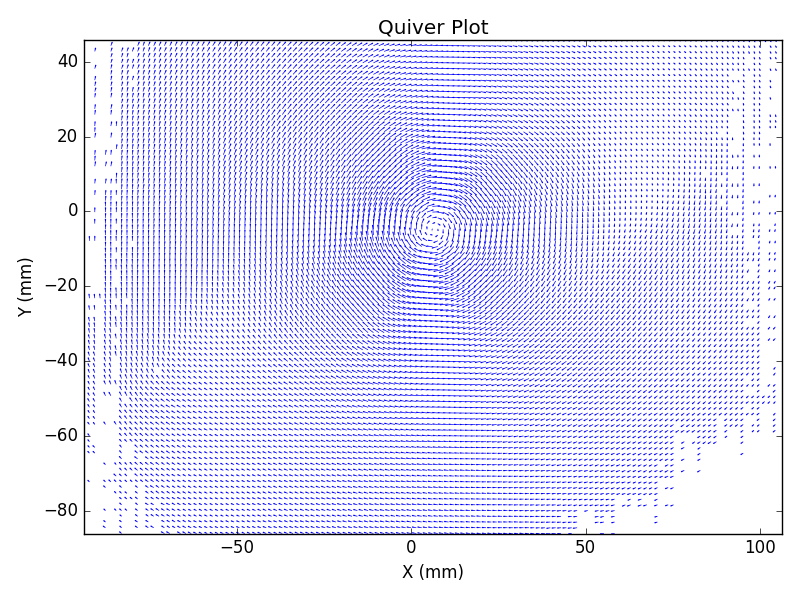
\includegraphics[width=5in]{figs/example_vortex_figs/example_quiver}
	\caption{Velocity vector field of a vortical flow structure as produced by 
	PIV.}
	\label{fig:quiver_example}
\end{figure}

 
\subsection{The Case for PIV}

Unlike other flow measurement techniques, PIV is considered to be a 
non-invasive method to directly measure particle displacements occurring during 
a precise time interval, and thus determine the particle velocity in the 
viewing plane. PIV is also capable 
of resolving vector measurements at many positions within a two dimensional 
slice of the flow field simultaneously, while other measurement techniques 
require taking data at many locations sequentially over a much longer period 
of time. PIV measurements can also be used to infer lift and drag forces on a 
solid body \cite{noca1997}. Single camera PIV can measure the two components of 
the velocity vectors aligned with the image plane, but the PIV method is 
capable of resolving many dimensions of fluid flow with incremental increases 
in system complexity. The addition of a second camera can enable the 
measurement of the three dimensional velocity vector, and a sweeping beam laser 
or holographic PIV architecture allows the interrogation of an entire volume of 
flow field instead of a "planar" slice 
\cite{barnhart1994,elsinga2006,kahler2000}.

Stereo PIV is used widely because it provides full velocity vector resolution, 
and requires only one additional camera and a slightly more complex 
calibration process and software to process the imagery. A stereo PIV system 
employing a  stationary sheet laser can resolve three dimensional mean velocity 
vectors and their associated fluctuations within a two dimensional slice of 
fluid flow. A 
two point correlation tensor containing important information about the 
turbulent structure of a flow can be obtained readily with PIV. The 
non-invasive nature of PIV, combined with the  ability to interrogate a flow 
volume very quickly for information with high dimensionality makes it 
exceptionally useful in fluid mechanics. \cite{adrian1991}

\subsubsection{PIV for the study of Turbulence}
The study of turbulent flows requires a large range of spatial and temporal 
velocity scales. Therefore, measurement techniques used to study turbulent 
phenomena require a significant spread between the lowest resolvable velocity, 
and the highest \cite{barnhart1994}. Although PIV has grown in popularity, it 
is not a complete replacement for more mature techniques including hot-wire 
anemometry. 
It has been shown that the attenuation of the velocity and velocity derivative 
statistics is significantly higher with PIV than with hot-wire anemometry due 
to the volume averaging associated with PIV techniques, and the aerodynamic and 
inertial behavior of the particles in the flow.
However, correction procedures have been developed that have been shown to 
allow corrected PIV measurements of turbulent kinetic energy to agree closely 
with hot-wire anemometry measurements \cite{lavoie2007,kasagi1991}. 

Reynolds stresses can be extracted from the two point correlations averaged 
over 
an interrogation window. With this technique, one Reynolds stress value can be 
obtained for each of the smallest interrogation windows, which are typically 
several pixels in size. In this technique, the particle displacements are found 
by finding the peak of the correlation function of image pairs, transformed 
into velocities and divided into mean and fluctuating components typical 
of a Reynolds averaging approach. Alternatively, single-pixel resolution 
Reynolds stress measurements can be obtained by direct examination of the 
correlation function. This technique can estimate Reynolds stresses at an 
enhanced resolution with errors on the order of a few percent when employing a 
set of several thousand PIV image pairs \cite{scharnowski2011}.

\subsection{Principles of Planar PIV}

A simple planar PIV system consists of a double pulsed laser, light sheet 
forming optics, particle seed, a single lens camera, image digitization 
hardware, and a computer system for data storage and subsequent analysis. The 
optical geometry of a planar PIV experiment is shown schematically in figure 
\ref{fig:mono_piv}.

\begin{figure}[H]
	\centering
	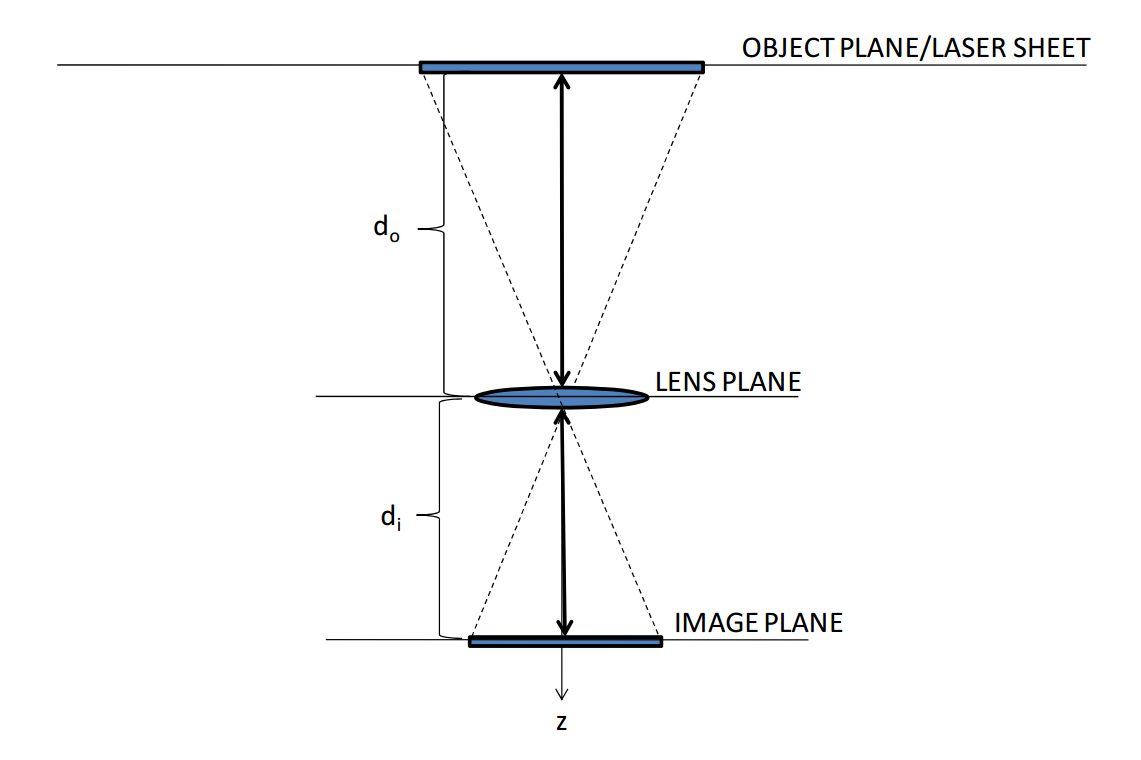
\includegraphics[width=5in]{figs/piv_method/mono_piv_optics}
	\caption{Single camera PIV system for mapping two dimensional velocity 
		vectors}
	\label{fig:mono_piv}
\end{figure} 

The 
underlying concept behind all PIV is that light scattered from the particles as 
they move through the illuminated flow field allows a pair of images to capture 
information about the motion of that particle. Double pulsed illumination is 
commonly employed in PIV systems due to its relatively low cost and simplicity
compared with multiple laser source systems. The energy required to adequately 
illuminate a planar area of interest depends upon the size of that area, and 
the scattering properties of the particle seed. Solid state Nd:YAG lasers are 
typically used for this purpose \cite{adrian2011}. An $(X, Y, Z)$ coordinate 
system is defined within the light sheet that exists in a so-called $(X, Y)$ 
space, and that can be related linearly to a 
coordinate system in the image plane of the camera in $(X_p, Y_p)$ pixel space. 
At a specific initiation time $t$, a laser light sheet is produced with a short 
duration pulse while the camera shutter is open to 
capture an image of the light scattering from particles within the flow domain. 
At some short time later, $t + dt$, a second light pulse occurs and a second 
image is taken. By measuring the pixel displacements $(\Delta X_p, \Delta 
Y_p)$ for a particle in the image plane, and transforming the coordinates into 
the plane of the laser sheet, one obtains $(\Delta X, \Delta Y, \Delta Z)$. 
This coordinate transform can be obtained from precise information about the 
optical geometry of the system, or by direct measurement of calibration data 
\cite{fouras2007}.The method of direct measurement of a calibration target was 
employed in this research. 

The detection rate, accuracy, and reliability of PIV depends upon careful 
selection of experimental parameters. \cite{keane1990} suggest a set of six 
important dimensionless quantities and ideal operating ranges that improve the 
chances of high quality PIV results . The parameters 
are: (1) data validation criterion, (2) particle image density, (3) relative 
in-plane image displacement, (4) relative out-of-plane displacement, (5) 
velocity gradient, and (6) the ratio of the mean image diameter to the 
interrogation spot diameter \cite{keane1990,lawson1997b}. Steep flow velocity 
gradients create random errors, because the 
individual particle displacements cover a discreet range within an 
interrogation spot. Particle displacements should be restricted to 25\% of the 
interrogation spot diameter for in-plane velocities, and to no more than 25\% 
of the light 
sheet thickness in out-of-plane velocities. One way to mitigate both of these 
limitations is to use as highest resolution PIV possible, or by scaling the 
interrogation area down by altering the zoom setting on the camera lenses. 
Since the velocity profile of an axial vortex can contain high velocity 
gradients in the vicinity of the core, and both in-plane and out-of-plane 
velocities are expected to be high, the present experiments used 50mm lenses to 
zoom each camera to focus on the smallest interrogation plane practical
\cite{prasad1992}.

\subsection{Principles of Stereo PIV}

Classical single camera PIV is only capable of capturing the projection of the 
velocity vector on the image plane. The out-of-plane component is lost 
completely, and the in-plane components are affected by unrecoverable error. In 
Stereo PIV, a pair of cameras may obliquely view the same plane and the entire 
three dimensional velocity vector can be inferred using the camera setup 
geometry. This technique 
includes tilting the backplanes of the cameras to satisfy the Scheimpflug image 
criteria and a dewarping function based on camera geometry to account for 
projective distortion \cite{willert1997}. An example of the geometric set up 
used by Willert to study the movement of a ring vortex through the 
interrogation plane is shown in Figure \ref{fig:stereo_piv}. Uncertainties 
associated with high out-of-plane motion in planar PIV are greatly reduced in 
stereo PIV \cite{lawson1997b,lawson1997}.

\begin{figure}[H]
	\centering
	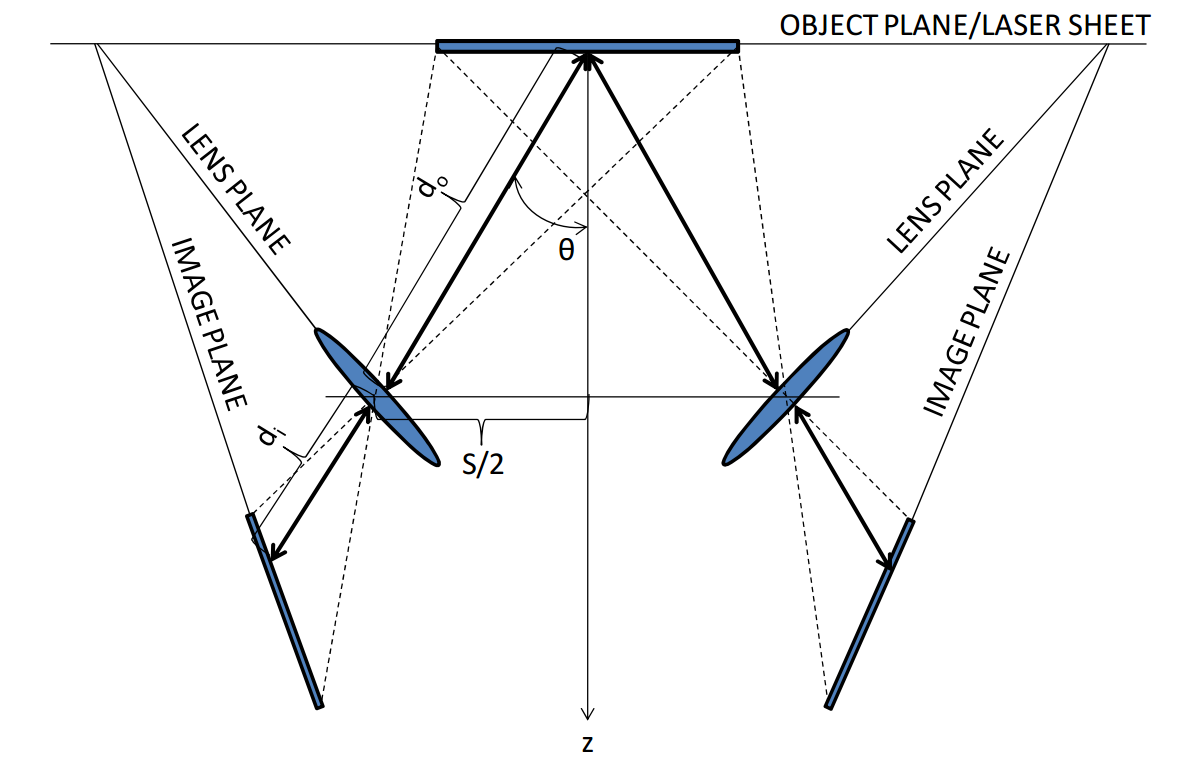
\includegraphics[width=5in]{figs/piv_method/stereo_piv_optics}
	\caption{Stereo camera PIV system for mapping three dimensional velocity 
		vectors}
	\label{fig:stereo_piv}
\end{figure}  

\subsection{Particles}

The "Particles" part of the PIV acronym refers to the small, highly reflective 
solid or liquid spheres that are entrained within a flow. It is assumed that 
the movement of the particles is representative of the fluid which propels them 
through the fluid, but this assumption deserves further examination 
\cite{roscoe1952}. Since particles have mass and ineertia, the particle motion 
is a function of the viscous forces exerted upon them by the fulid, and by 
gravitational or magnetic body forces. As a particle is convected with the 
fluid and the local fluid encounters a change in direction, the particle cannot 
respond instantaneously. The exact response to rapid changes in velocity in the 
transporting fluid is of great interest to the study of turbulence.It has been 
found that lightweight 
particles have a tendency to collect in regions of high strain rate and low 
vorticity. However, extremely light particles exhibit weaker preferential 
concentration effects because they follow the fluid motion more closely, while 
relatively heavy particles become virtually insensitive to turbulent velocity 
fluctuations \cite{squires1990}. Evidence of preferential particle collection 
can be seen in wake vortex PIV, where the vortex core is identifiable as a 
small spot of lower particle density as in Figure 
\ref{fig:vortex_core_particles}.
	
\begin{figure}
	\centering
	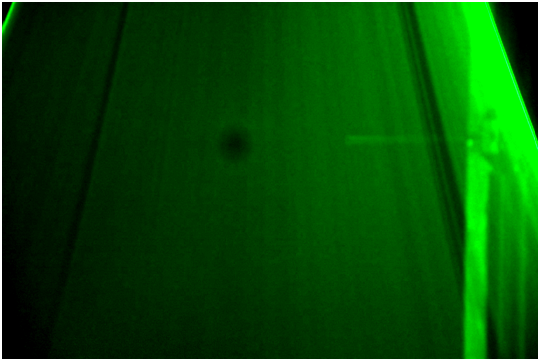
\includegraphics[width=4in]{figs/piv_method/vortex_core}
	\caption{Contrast enhanced image of an illuminated cross section showing a 
	low particle density in the vortex core.}
	\label{fig:vortex_core_particles}
\end{figure}

As the characteristic inertia and diameter of seed particles shrinks, they 
become capable of following 
smaller turbulent length scales, but the prime consideration for particles 
becomes the ability of a camera system to detect the light which scatters from 
them. The intensity of the light reflecting from a 
particles should be sufficient to reach 30\% to 50\% of the saturation level of 
the recording device. The controlling factors for intensity of reflected light 
are particle size, laser power, and refractive index \cite{adrian2011}. Thus, 
particles which are small enough to ensure sensitivity to turbulent structures 
on the time and length scales of interest must be small enough to respond to 
those turbulent fluctuation scales, but large enough to be detected. It has 
been demonstrated that particle dimensions of one micrometer with densities 
between 0.56 and 1.62 times the density of the fluid enable the particles to 
respond accurately to turbulent structures in air on the order of many thousand 
Hertz \cite{mei1996}. In the 
present study, $CO_2$ filled mineral oil bubbles generated with an MDG MAX 3000 
APS fog generator with a Laskin 
nozzle were used as particle seed. These droplets have a nominal 
diameter of 0.6 micrometers and densities of 1.55 times that of air were used 
\cite{mdgfog}.

The density of particle seeding must be sufficient for a correlation to be 
generated between frames for every small interrogation spot in the survey 
plane. In an instance where only one or two particles are visible in the first 
frame at the edge of an interrogation sector, then those particles exit the 
sector for the second frame, to be replaced by new particles 
entering the area from the other side, spurious results will be produced.


\subsection{Image processing}

There are multiple methods for extracting vector fields from images of 
particles. A commonality between all methods is the use of a correlation 
function to find particle displacements. The correlation map is computed by 
taking the inverse fast Fourier transform (FFT) of the product of the FFT of 
the first image, and the complex conjugate of the FFT of the second image, then 
adjusting for up-sampling by dividing by the original factor as in equation. 
Displacement is measured by finding the peak of correlation map between a small 
sector of each image, represented by Equation \ref{eq:correlation_map}. 

\begin{equation}
C_{map} = FFT^{-1} * [F_A \times conj(F_B) ]
\label{eq:correlation_map}
\end{equation}

where $C_{map}$ is the correlation map, $F_A$ is the fast Fourier transform of 
image $A$, at time $t=0$ and $F_B$ is the fast Fourier transform of image $B$ 
at time $t=dt$. This process is repeated many times to create a vector field of 
pixel displacements. In the simplest case, these correlation maps are 
considered individually, and the absolute highest peak is used to determine the 
mean pixel displacement within a sector. The Hart method, which was used in the 
present study, improves upon this with element by element comparison of 
adjacent sectors correlation tables to remove false peaks 
\cite{hart1998,hart1999}.

The mathematics behind derivation of velocity vector fields from stereo image 
pairs is based upon coordinate transformations from pixel coordinates to real 
coordinates with the following Equations 
\ref{eq:piv_to_real1} to \ref{eq:piv_to_real4}.

\begin{equation}
x_L= X\frac{dx_L}{dX} + Y\frac{dx_L}{dY} + Z\frac{dx_L}{dZ}
\label{eq:piv_to_real1}
\end{equation}

\begin{equation}
x_R= X\frac{dx_R}{dX} + Y\frac{dx_R}{dY} + Z\frac{dx_R}{dZ}
\label{eq:piv_to_real2}
\end{equation}

\begin{equation}
y_L= X\frac{dy_L}{dX} + Y\frac{dy_L}{dY} + Z\frac{dy_L}{dZ}
\label{eq:piv_to_real3}
\end{equation}

\begin{equation}
y_R= X\frac{dy_R}{dX} + Y\frac{dy_R}{dY} + Z\frac{dy_R}{dZ}
\label{eq:piv_to_real4}
\end{equation}

where $x_L$, $x_R$, $y_L$ and $y_R$ are the pixel displacements in the x 
direction on the left and right cameras, and the y direction on the left and 
right cameras respectively. Symbols $X$, $Y$, and $Z$ are real spatial particle 
displacements in the interrogation plane. The set of twelve derivatives are 
pixel displacement sensitivity coefficients, which are determined by a 
calibration process which involves taking pictures of a matrix of bright dots 
with a known distance between each dot. Once all twelve calibration 
coefficients are known, the set of equations is actually over constrained, with 
four equations and only three unknowns, a least squared method will be used to 
map measurements form the image plane to the real plane. In the case of this 
study, INSIGHT software was used to generate this set of calibration 
coefficients.

The image is 
up sampled to higher resolution to allow sub-pixel displacements to be 
measured, thus preventing accuracy limitations associated with the physical 
dimensions of each pixel. The image is typically divided into grids 16 by 16 
pixels in size, with 50\% overlap with surrounding grids to ensure particles 
which started inside the sector at $t=0$, but begin to exit the sector at 
$t=dt$, are still identifiable.  


Figure \ref{fig:piv_sector_0up} shows a sample of two side by side images taken 
several microseconds, $dt$ apart without any up-sampling. Figure 
\ref{fig:piv_sector_overlay_fft_0up} shows a sample of the same two images 
layered on top of each other to show the apparent horizontal displacement 
between the two images. The two dimensional correlation map shows a clear peak 
down at four pixels in the $X$ direction and zero pixels in the $Y$ direction.


\begin{figure}[H]
	\begin{subfigure}{.49\textwidth}
		\centering
		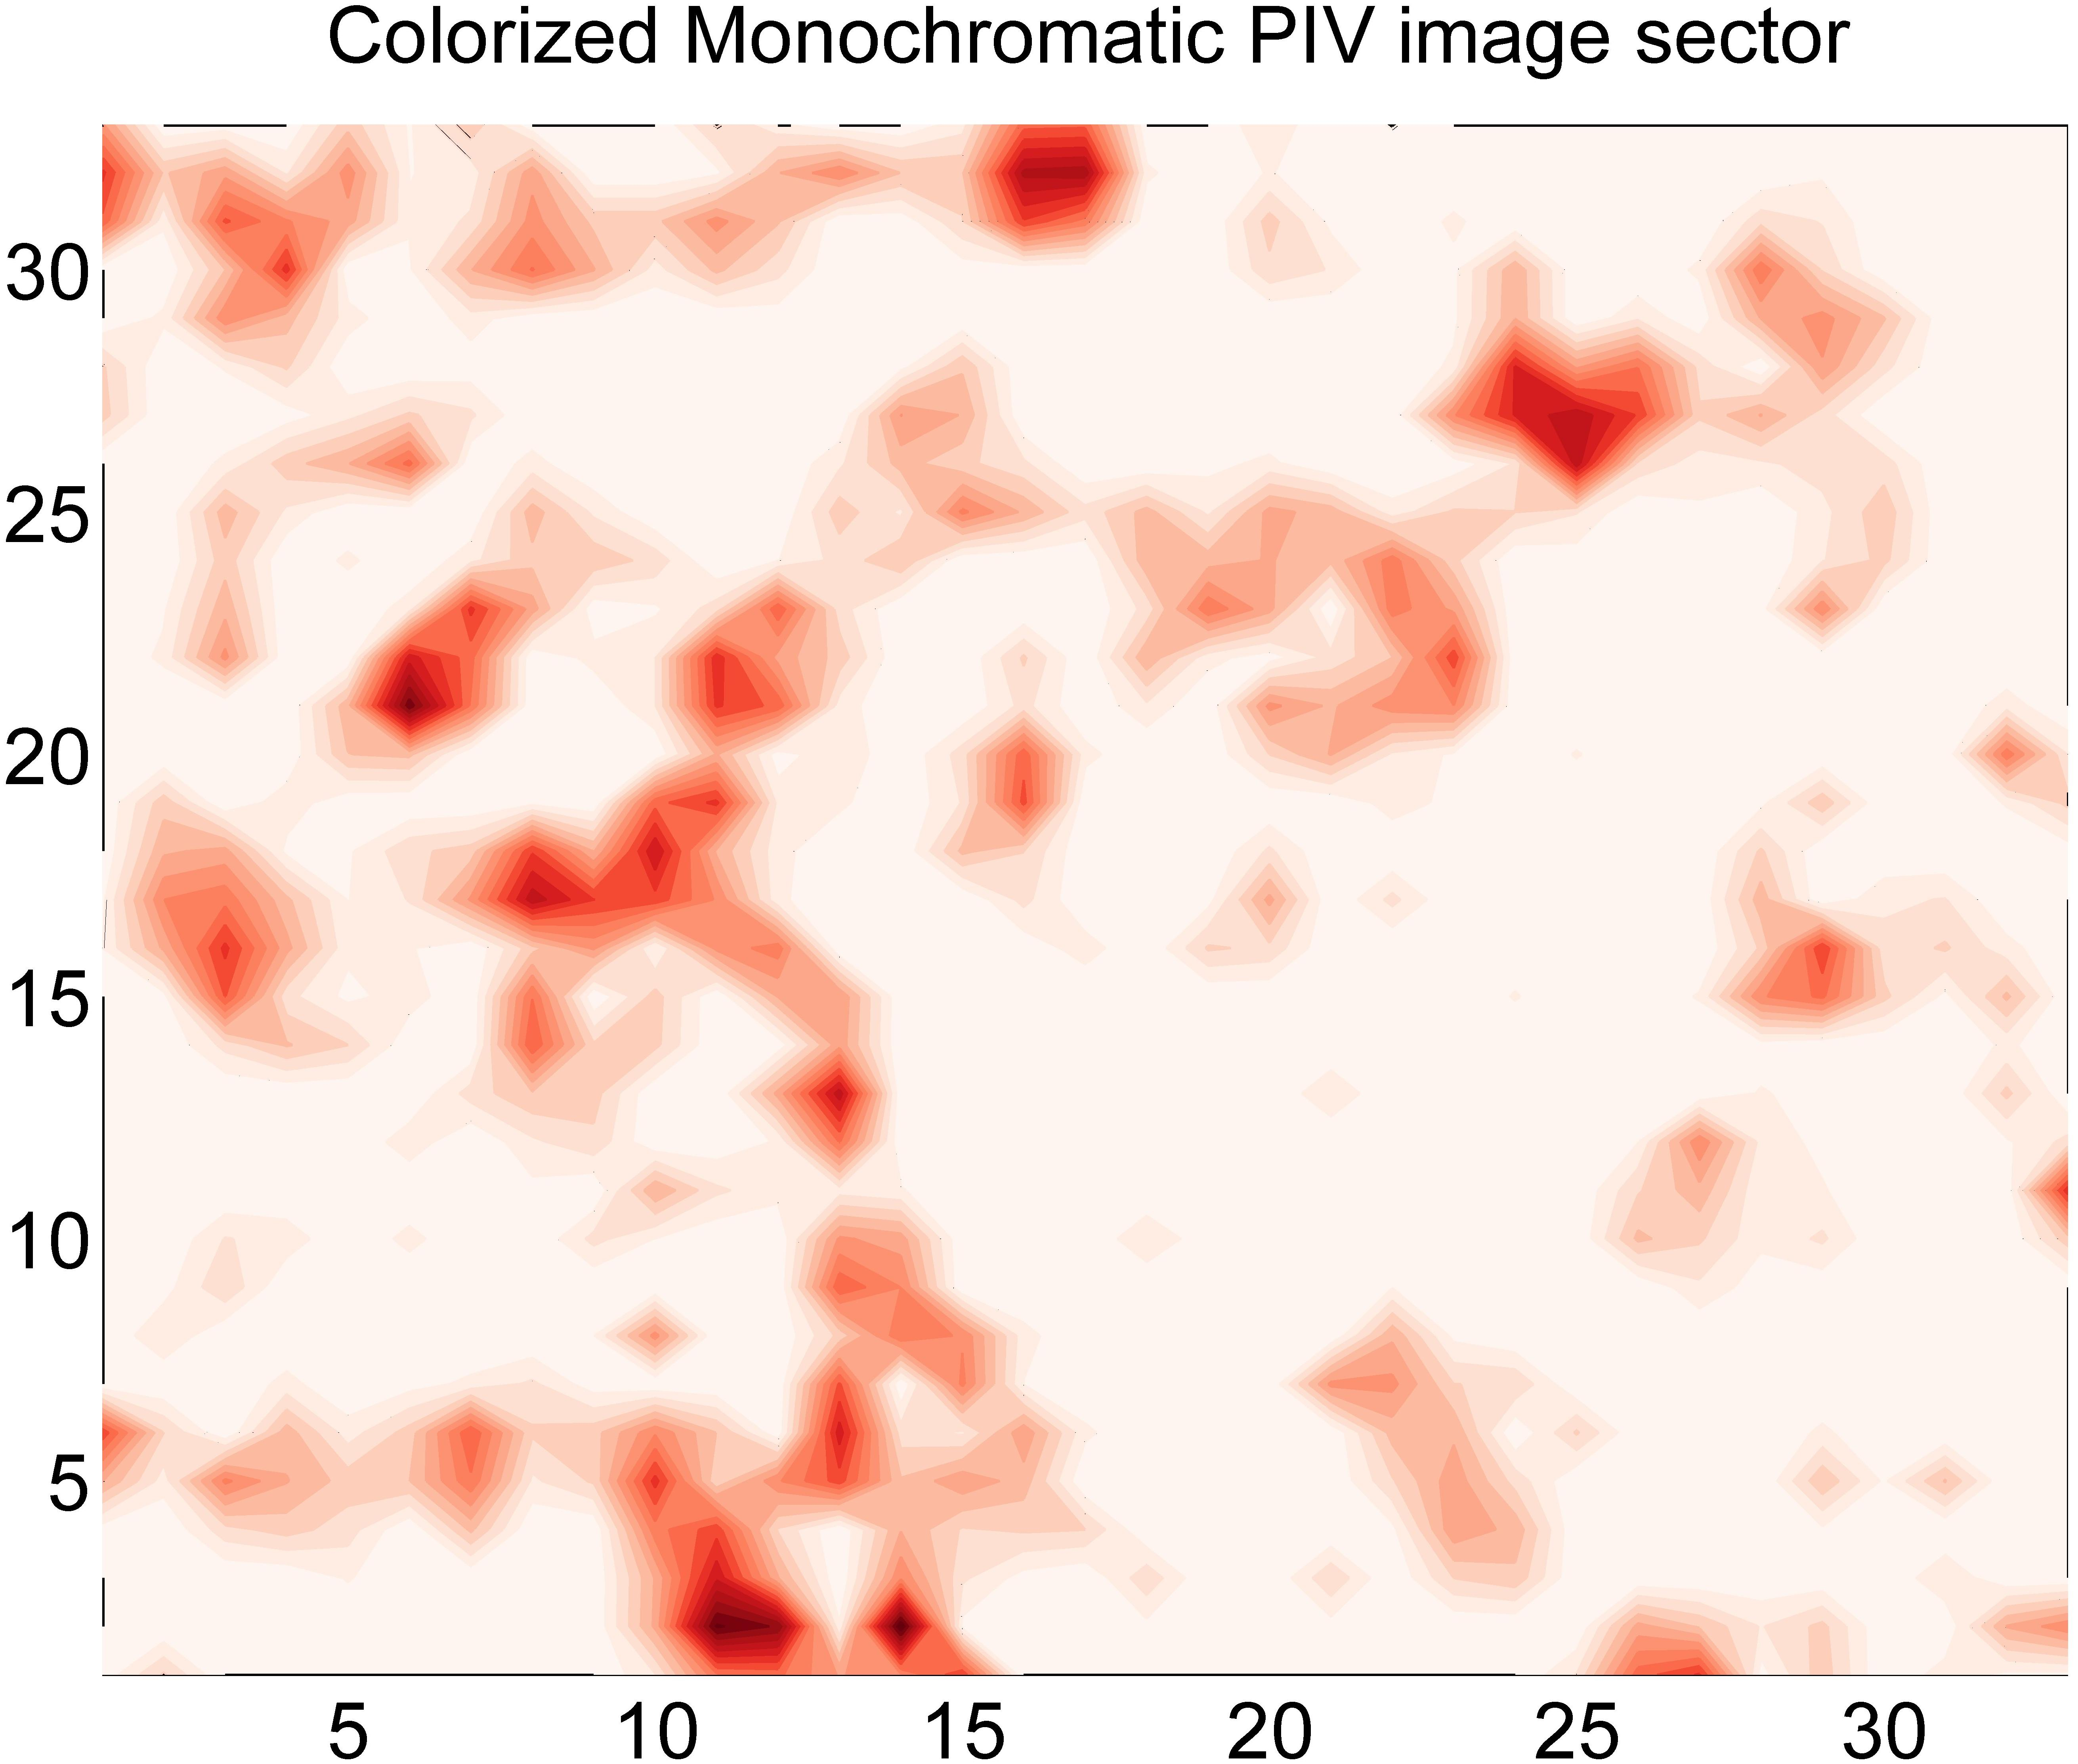
\includegraphics[width=.9\linewidth]{figs/piv_method/pive_figa_order0}
	\end{subfigure} 
	\begin{subfigure}{.49\textwidth}
		\centering
		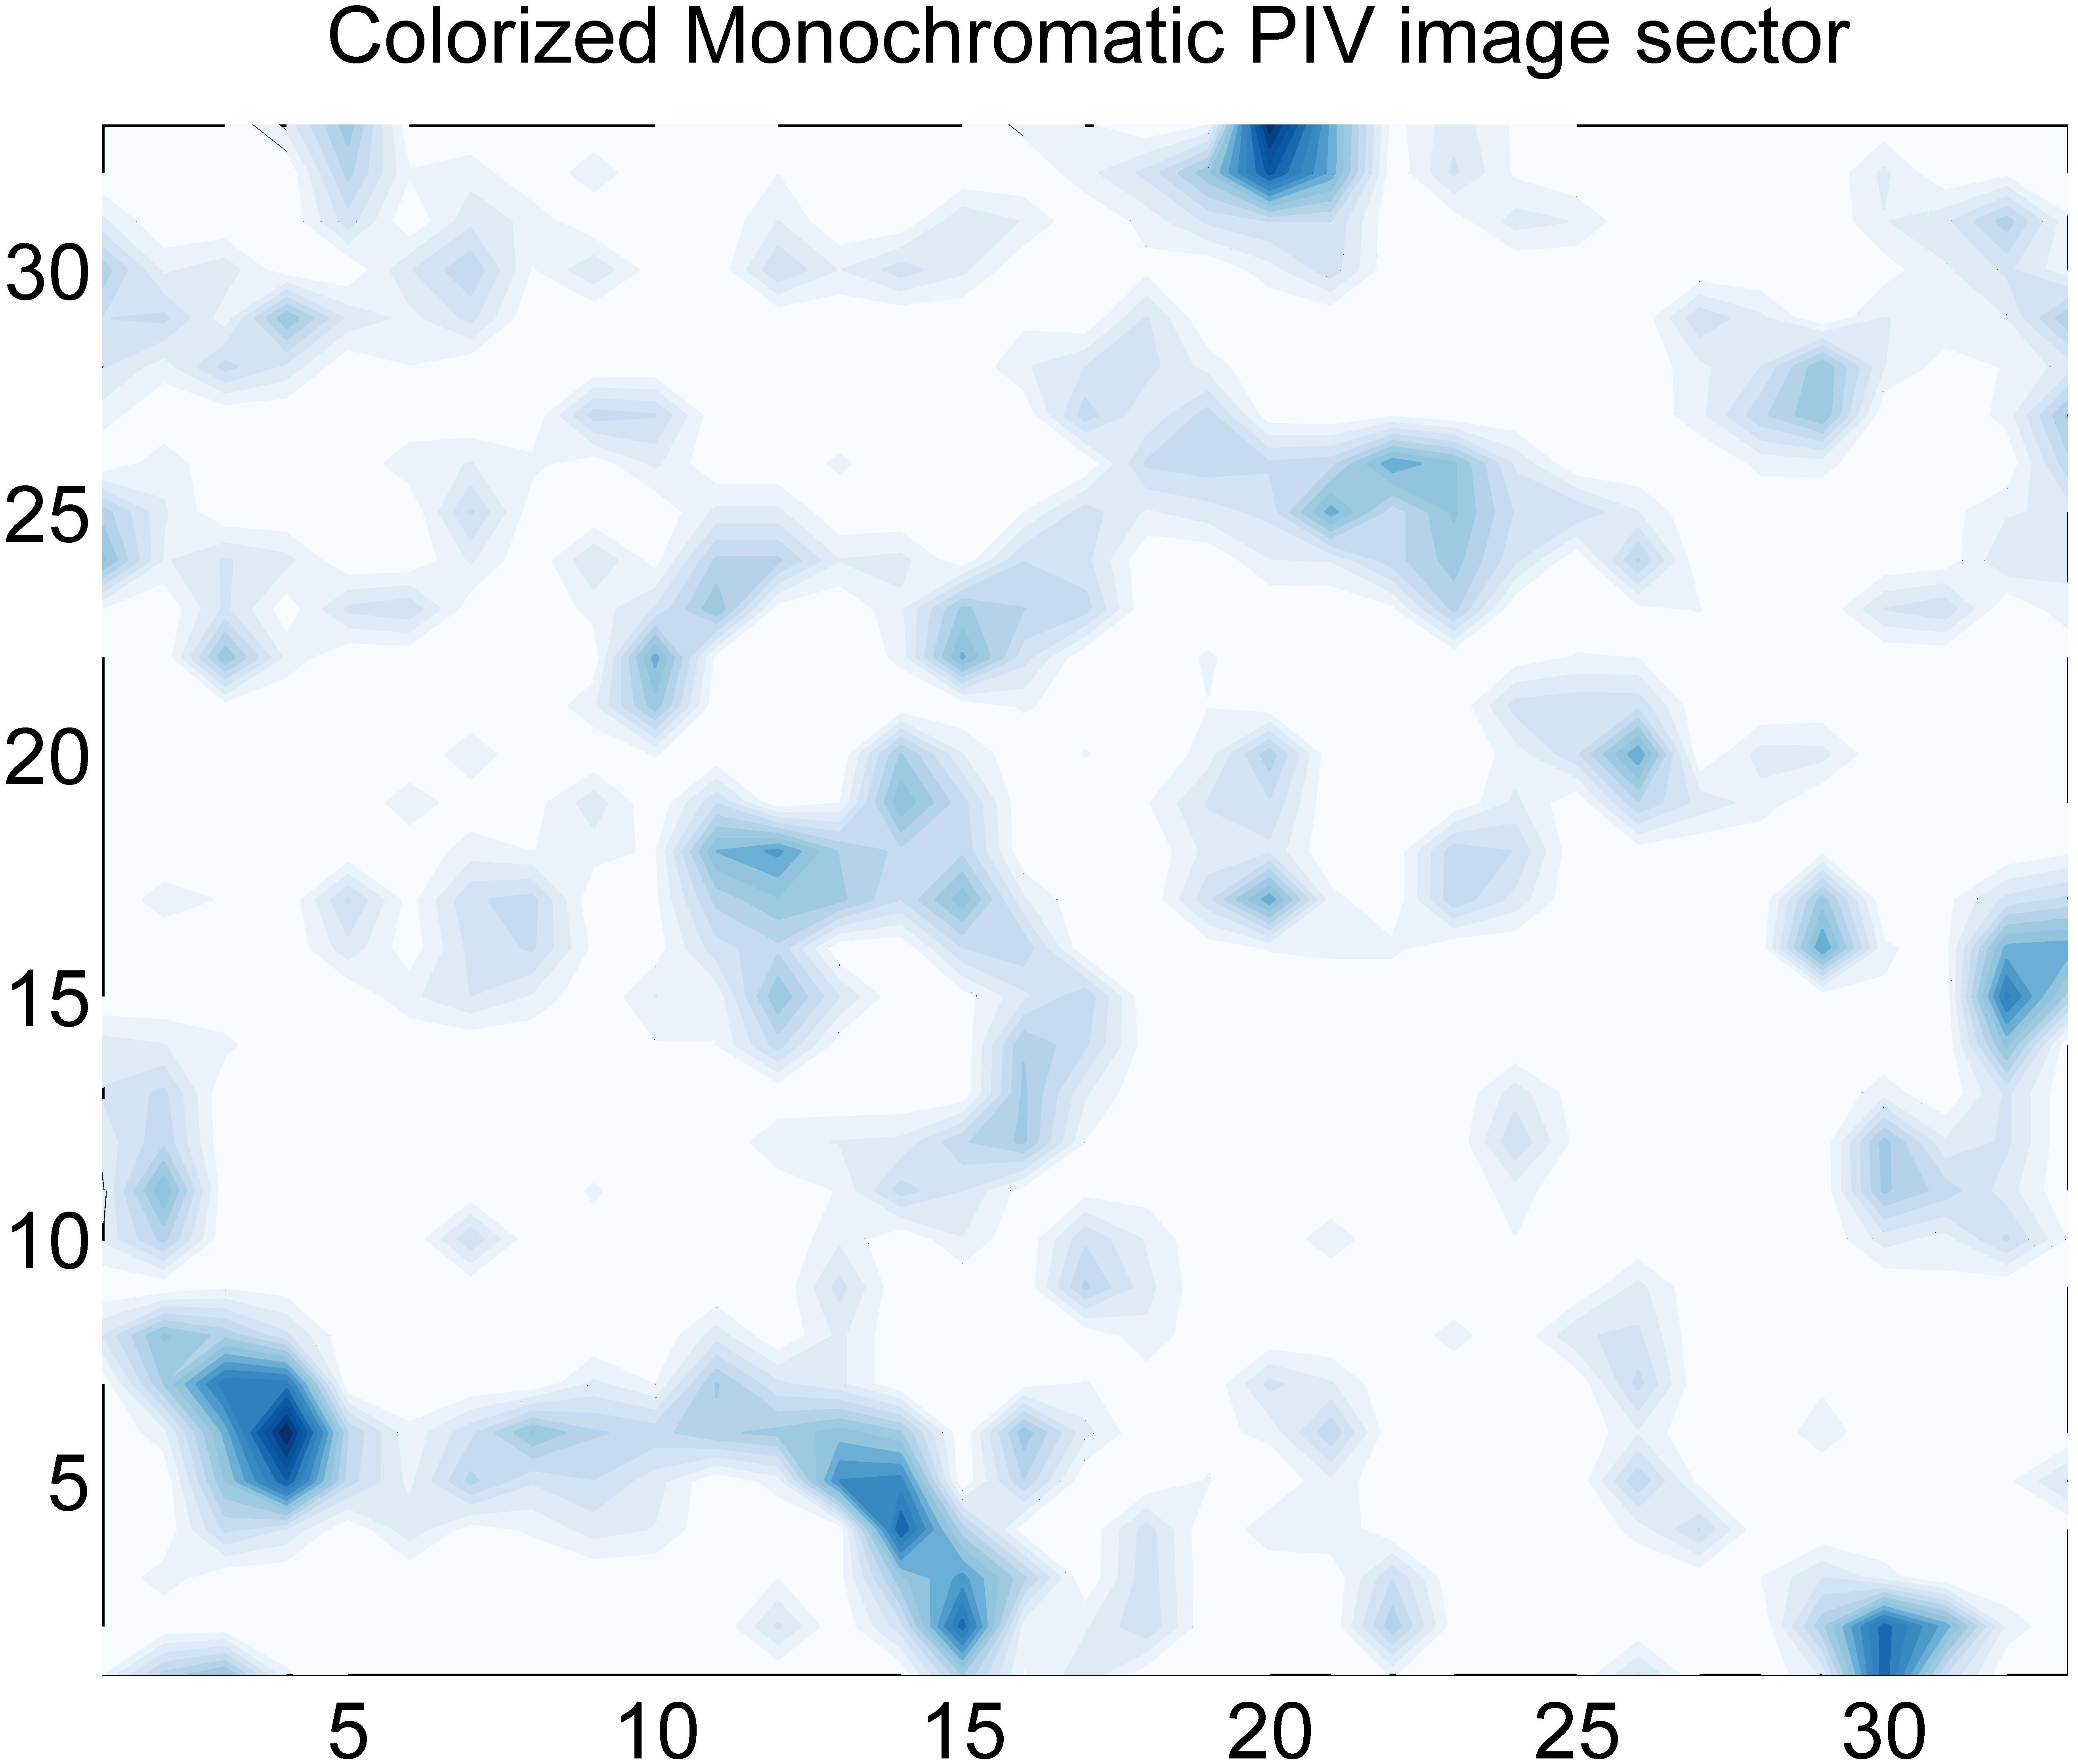
\includegraphics[width=.9\linewidth]{figs/piv_method/pive_figb_order0}
	\end{subfigure}	
	\caption{Colorized 32x32 pixel contour images at $t=0$ (left), and $t=dt$ 
		(right), no up sampling.}
	\label{fig:piv_sector_0up}
\end{figure}


\begin{figure}[H]
	\begin{subfigure}{.49\textwidth}
		\centering
		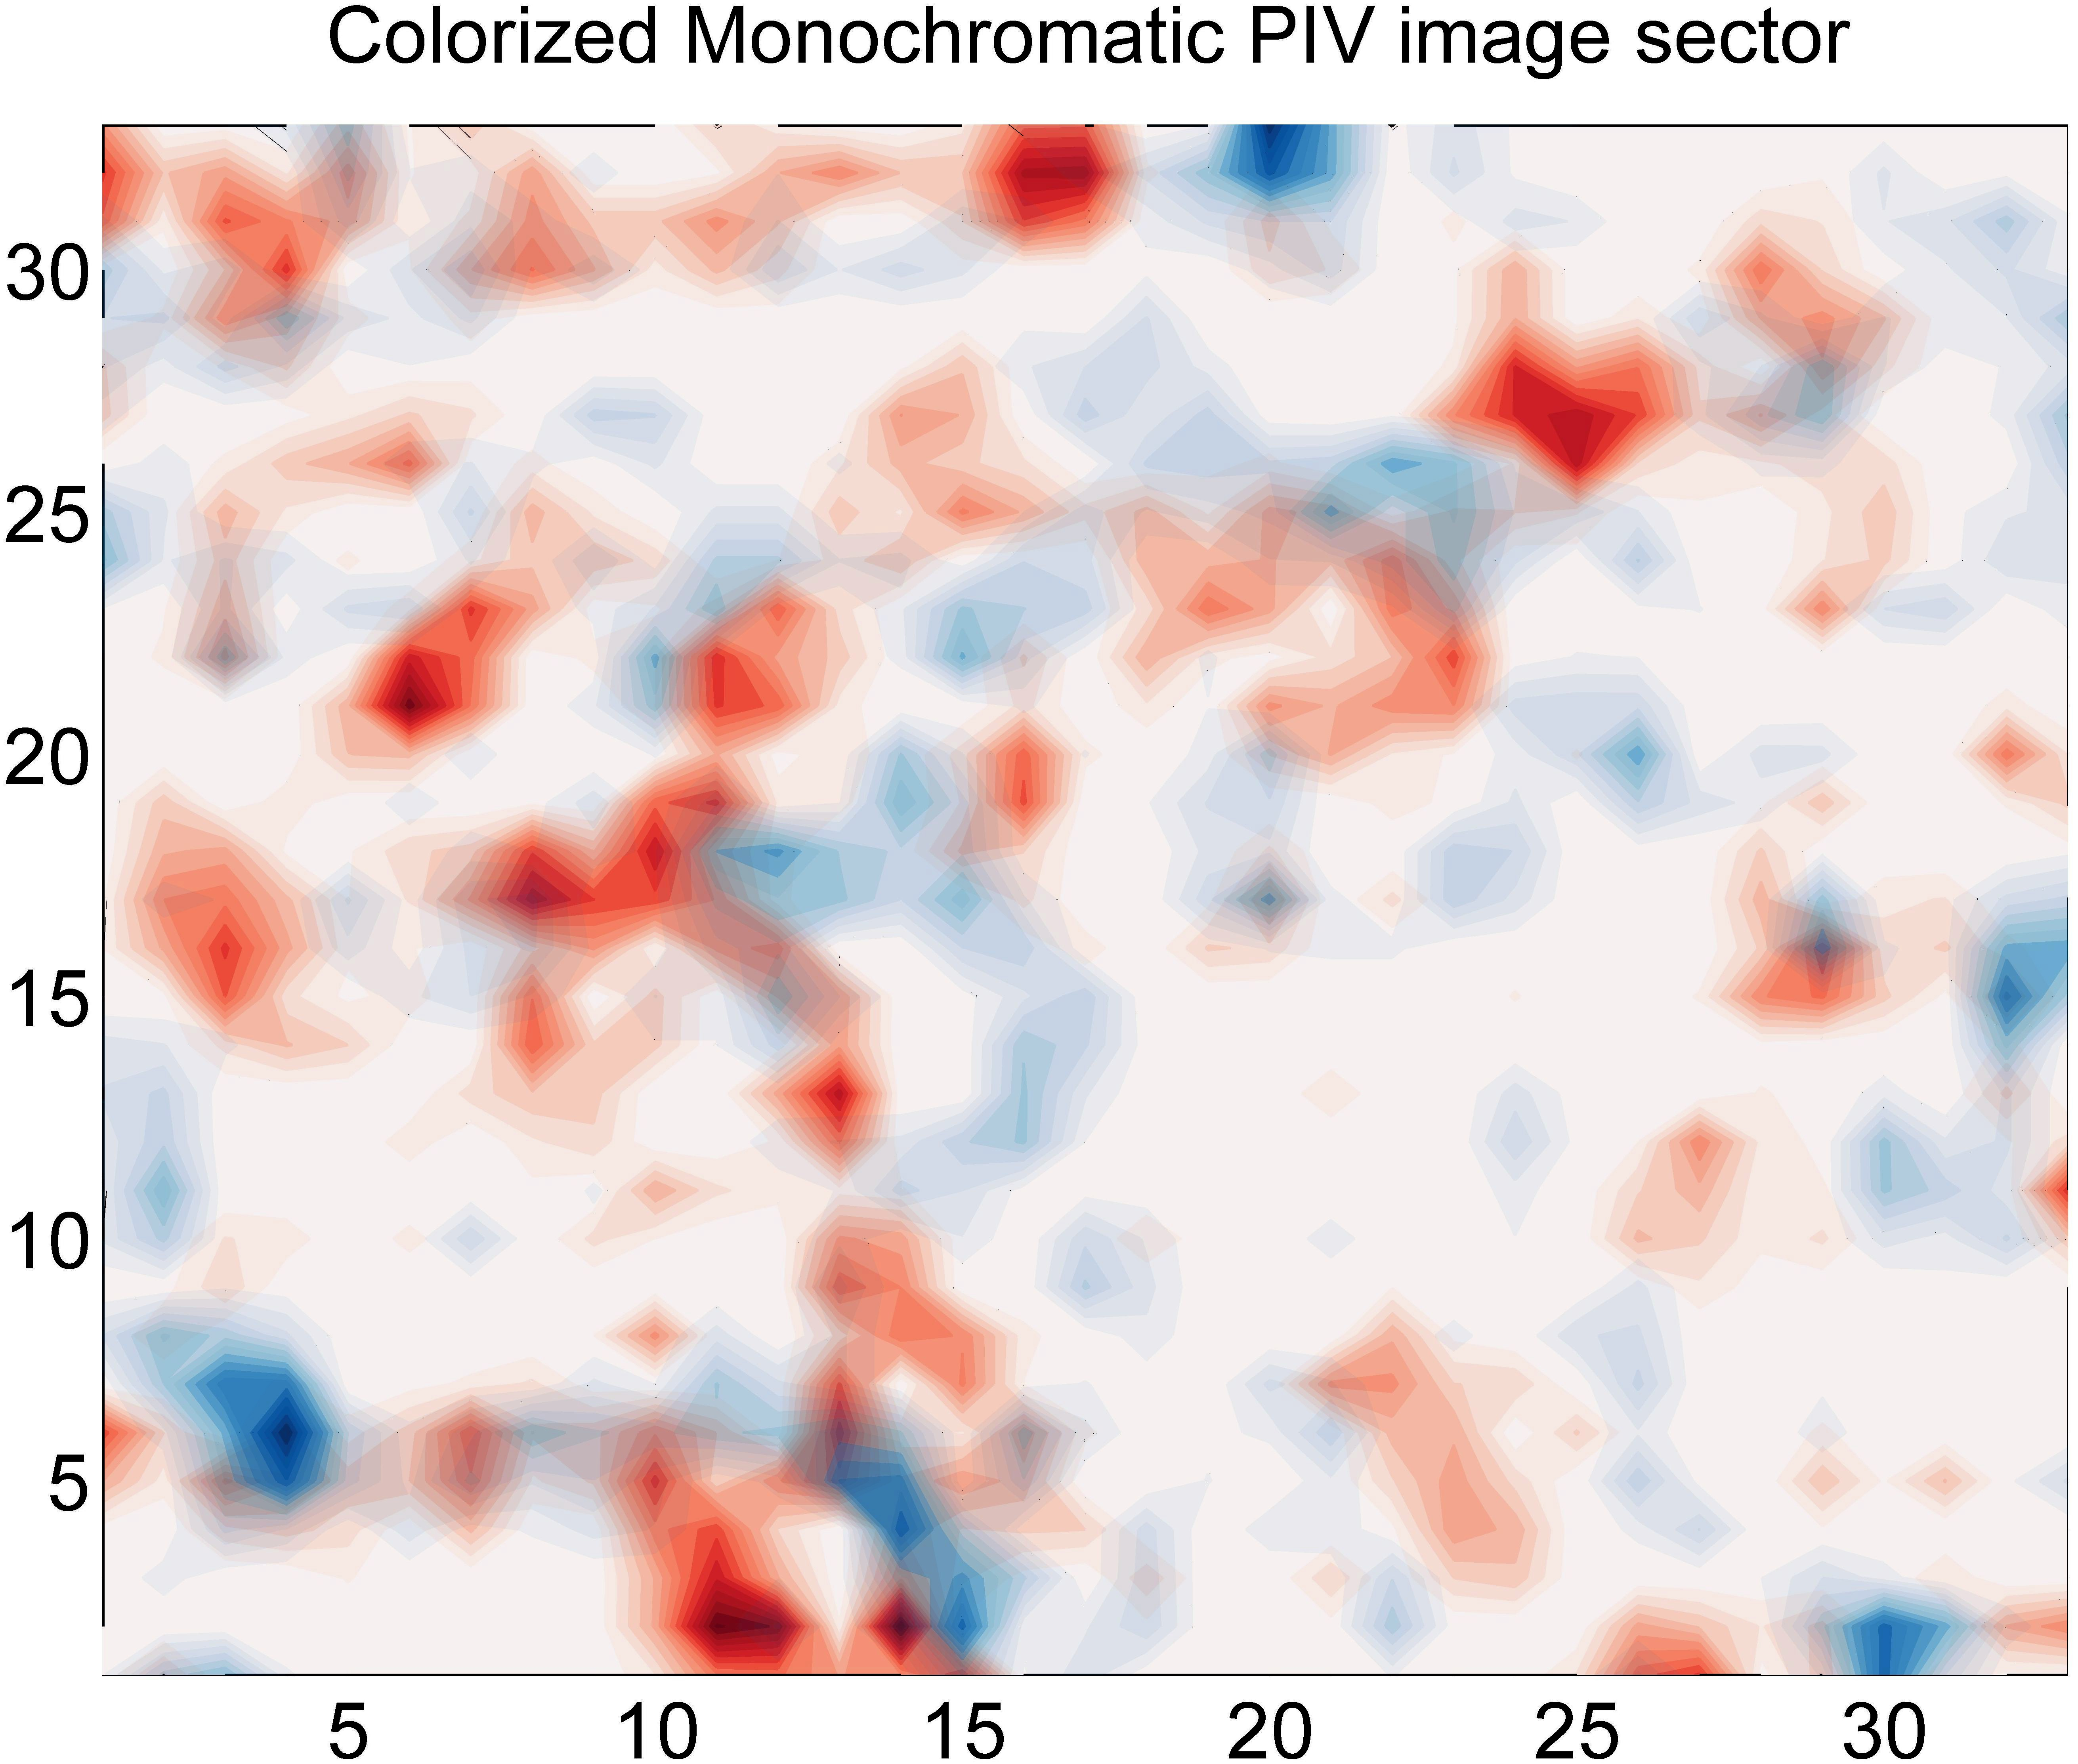
\includegraphics[width=.9\linewidth]{figs/piv_method/pive-fig_order0}
	\end{subfigure} 
	\begin{subfigure}{.49\textwidth}
		\centering
		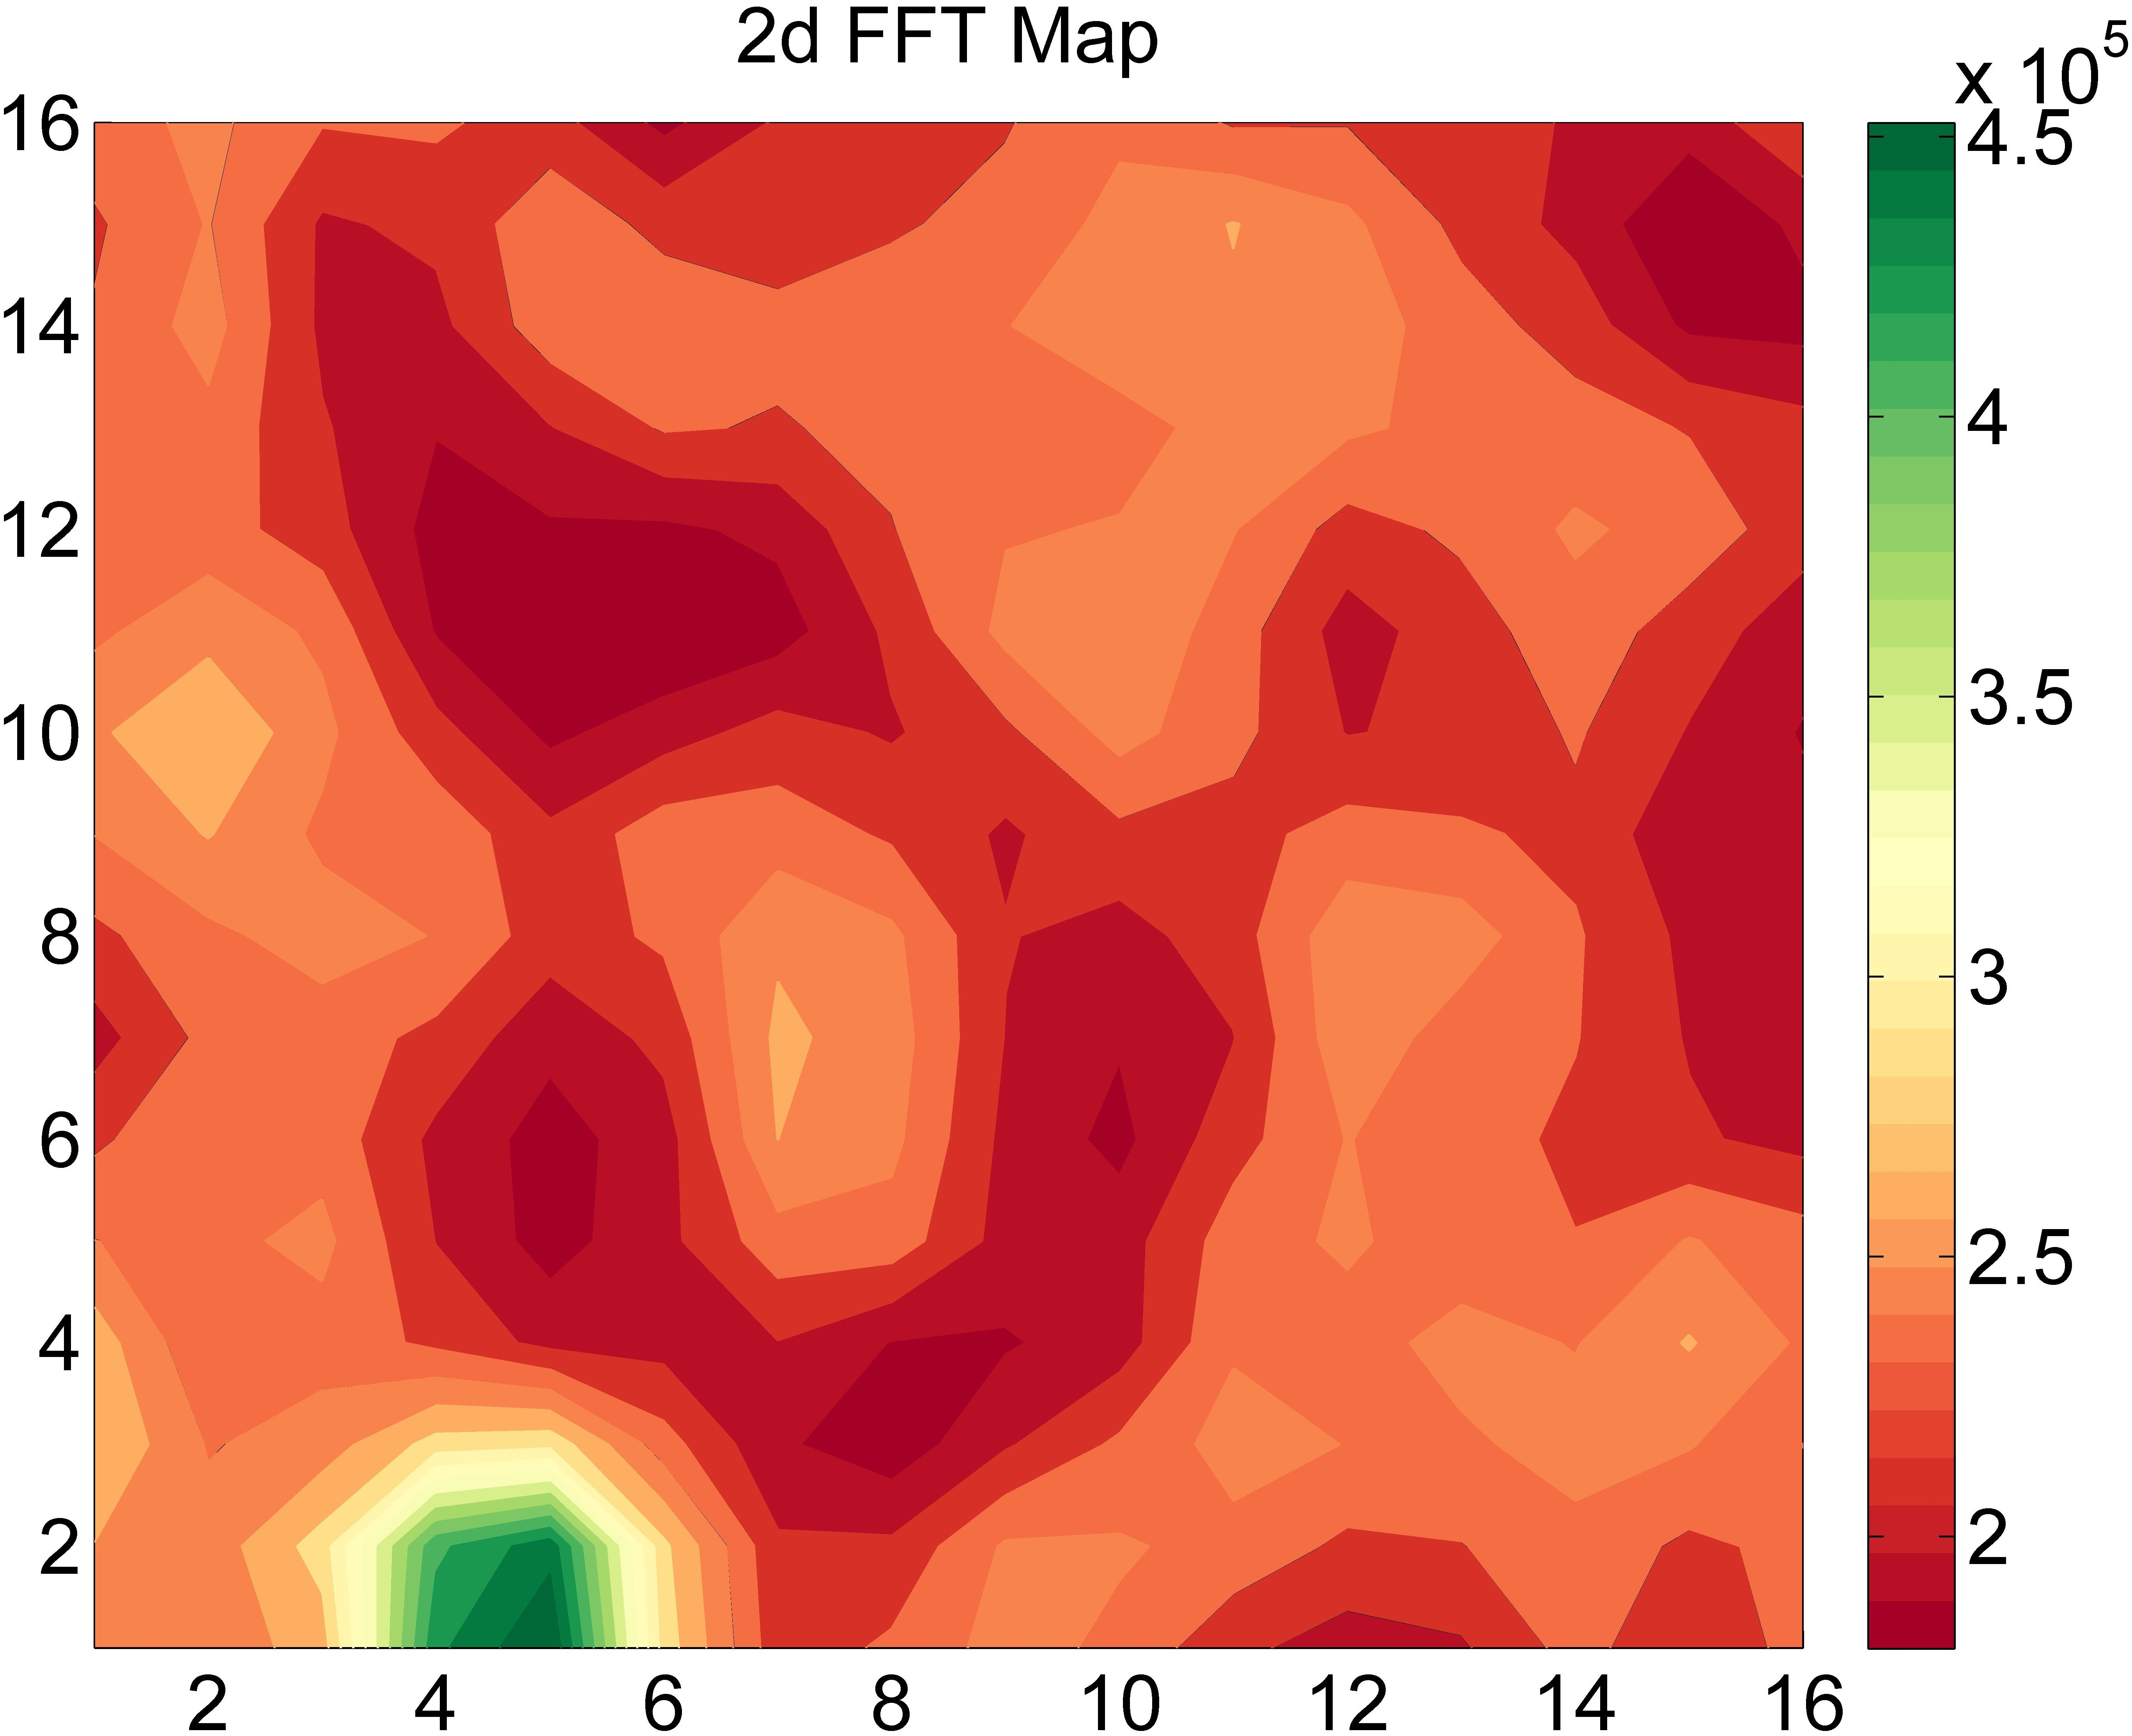
\includegraphics[width=.9\linewidth]{figs/piv_method/pive_fft_order0}
	\end{subfigure}	
	\caption{Overlaid sector snapshots (left) and corresponding correlation 
		map (right), no up sampling.}
	\label{fig:piv_sector_overlay_fft_0up}
\end{figure}


Every up sampling doubles the dimensions of the sector, quadrupling the number 
of pixels and increasing the sub-pixel resolution by a factor of two. The same 
set of figures is repeated for the same image with 6th order bilinear up 
sampling in figures \ref{fig:piv_sector_6up} and
\ref{fig:piv_sector_overlay_fft_6up}. Note that the images are much smoother, 
and the images have been sampled sufficiently to make a very finely spaced grid.
It is important to note that while bilinear up sampling is used for this
example, any other two dimensional method such as cubic may be used.

\begin{figure}[H]
	\begin{subfigure}{.49\textwidth}
		\centering
		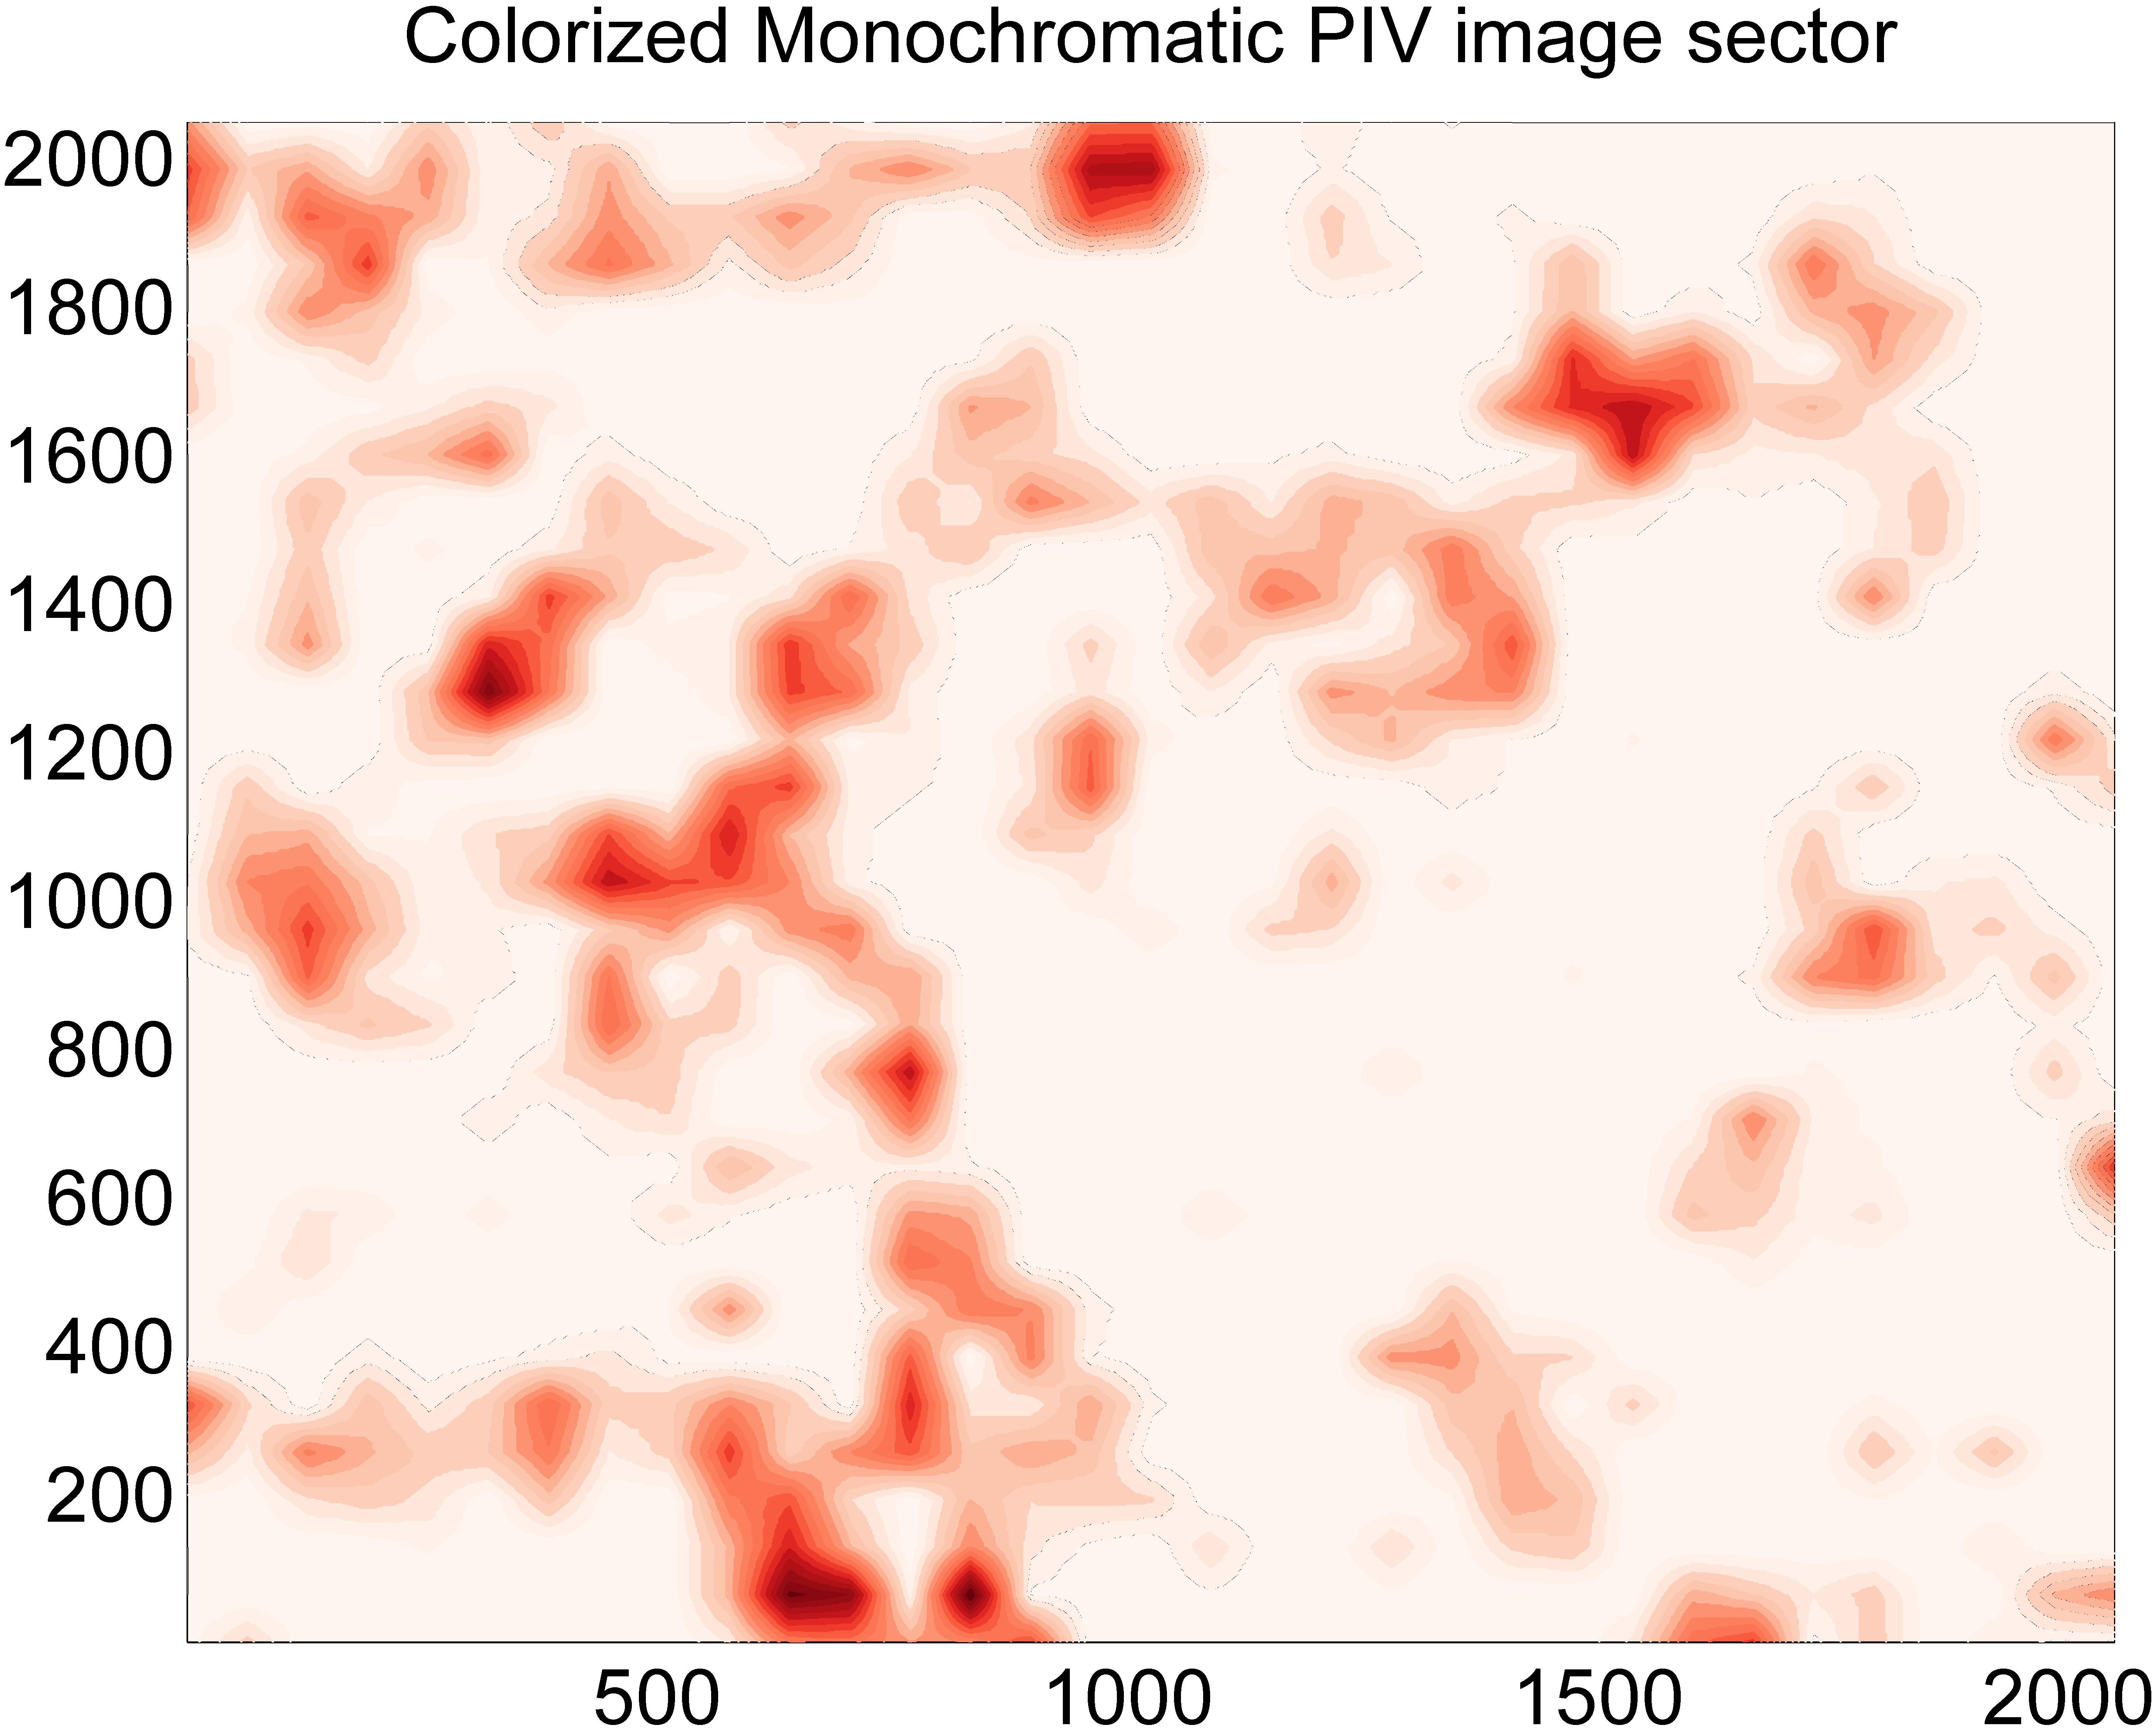
\includegraphics[width=.9\linewidth]{figs/piv_method/pive_figa_order6}
	\end{subfigure} 
	\begin{subfigure}{.49\textwidth}
		\centering
		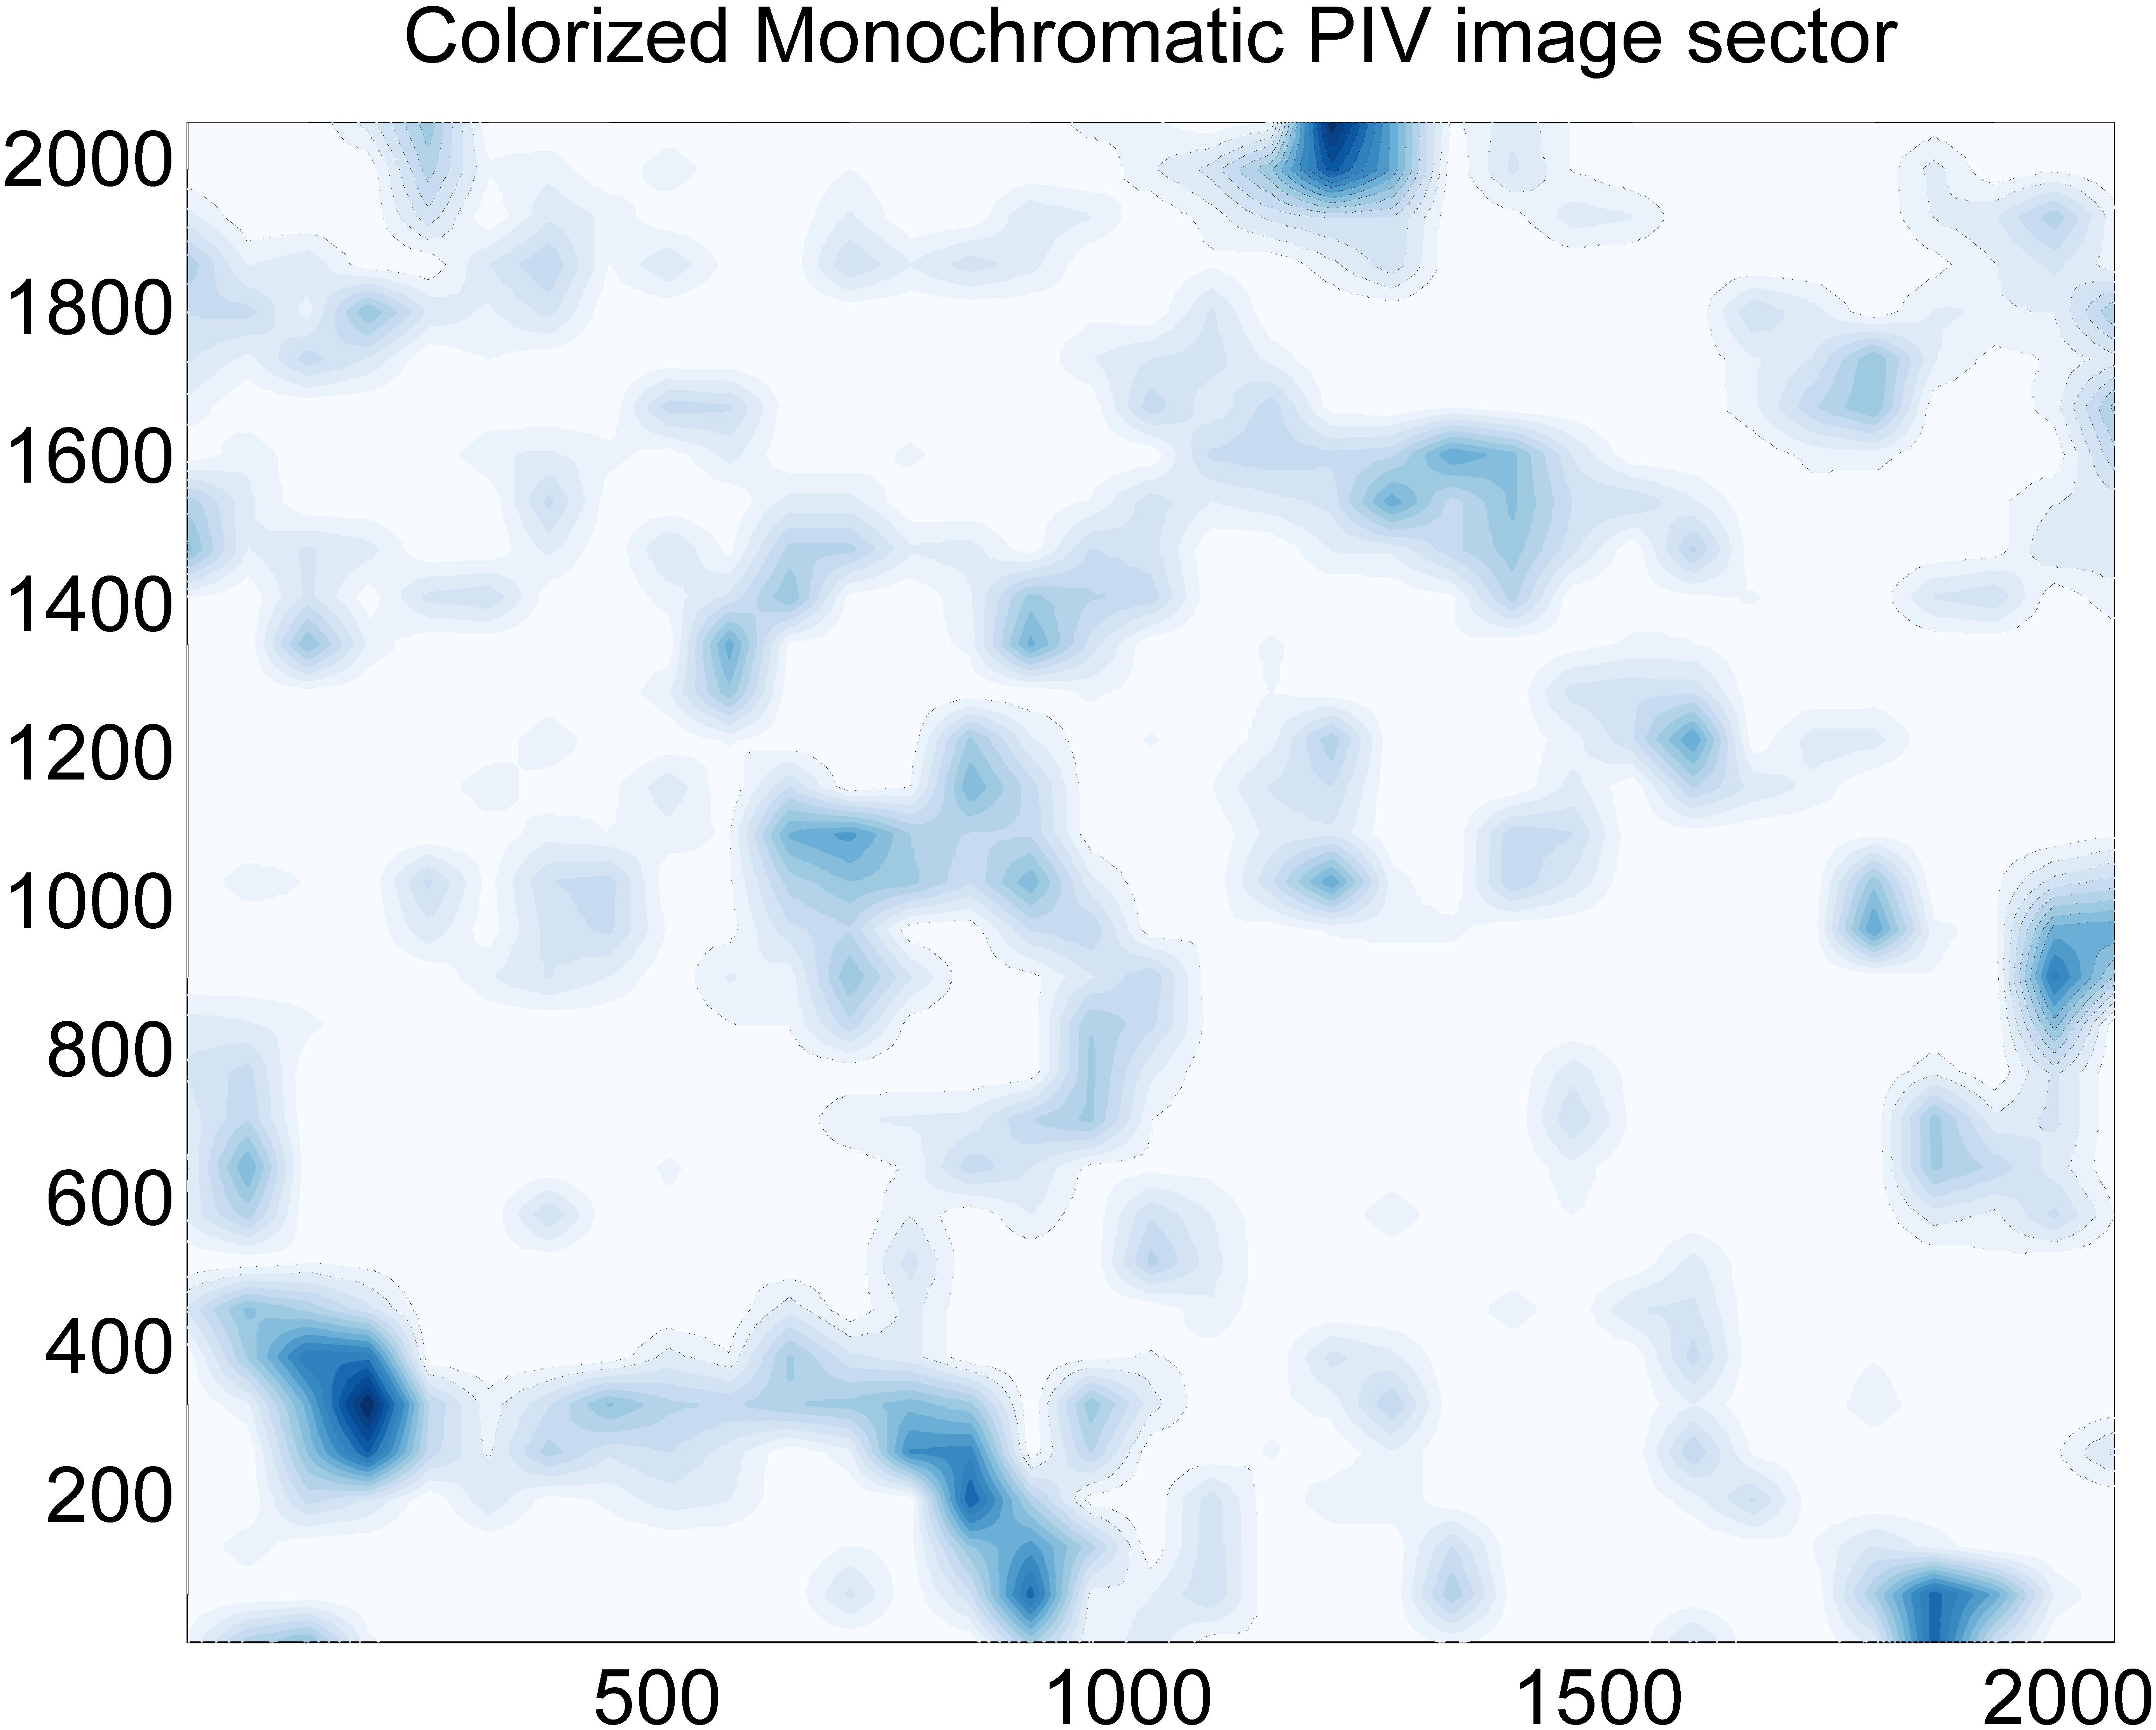
\includegraphics[width=.9\linewidth]{figs/piv_method/pive_figb_order6}
	\end{subfigure}	
	\caption{Colorized 32x32 pixel contour images at $t=0$ (left), and $t=dt$ 
		(right), 6th order up sampling.}
	\label{fig:piv_sector_6up}
\end{figure}


\begin{figure}[H]
	\begin{subfigure}{.49\textwidth}
		\centering
		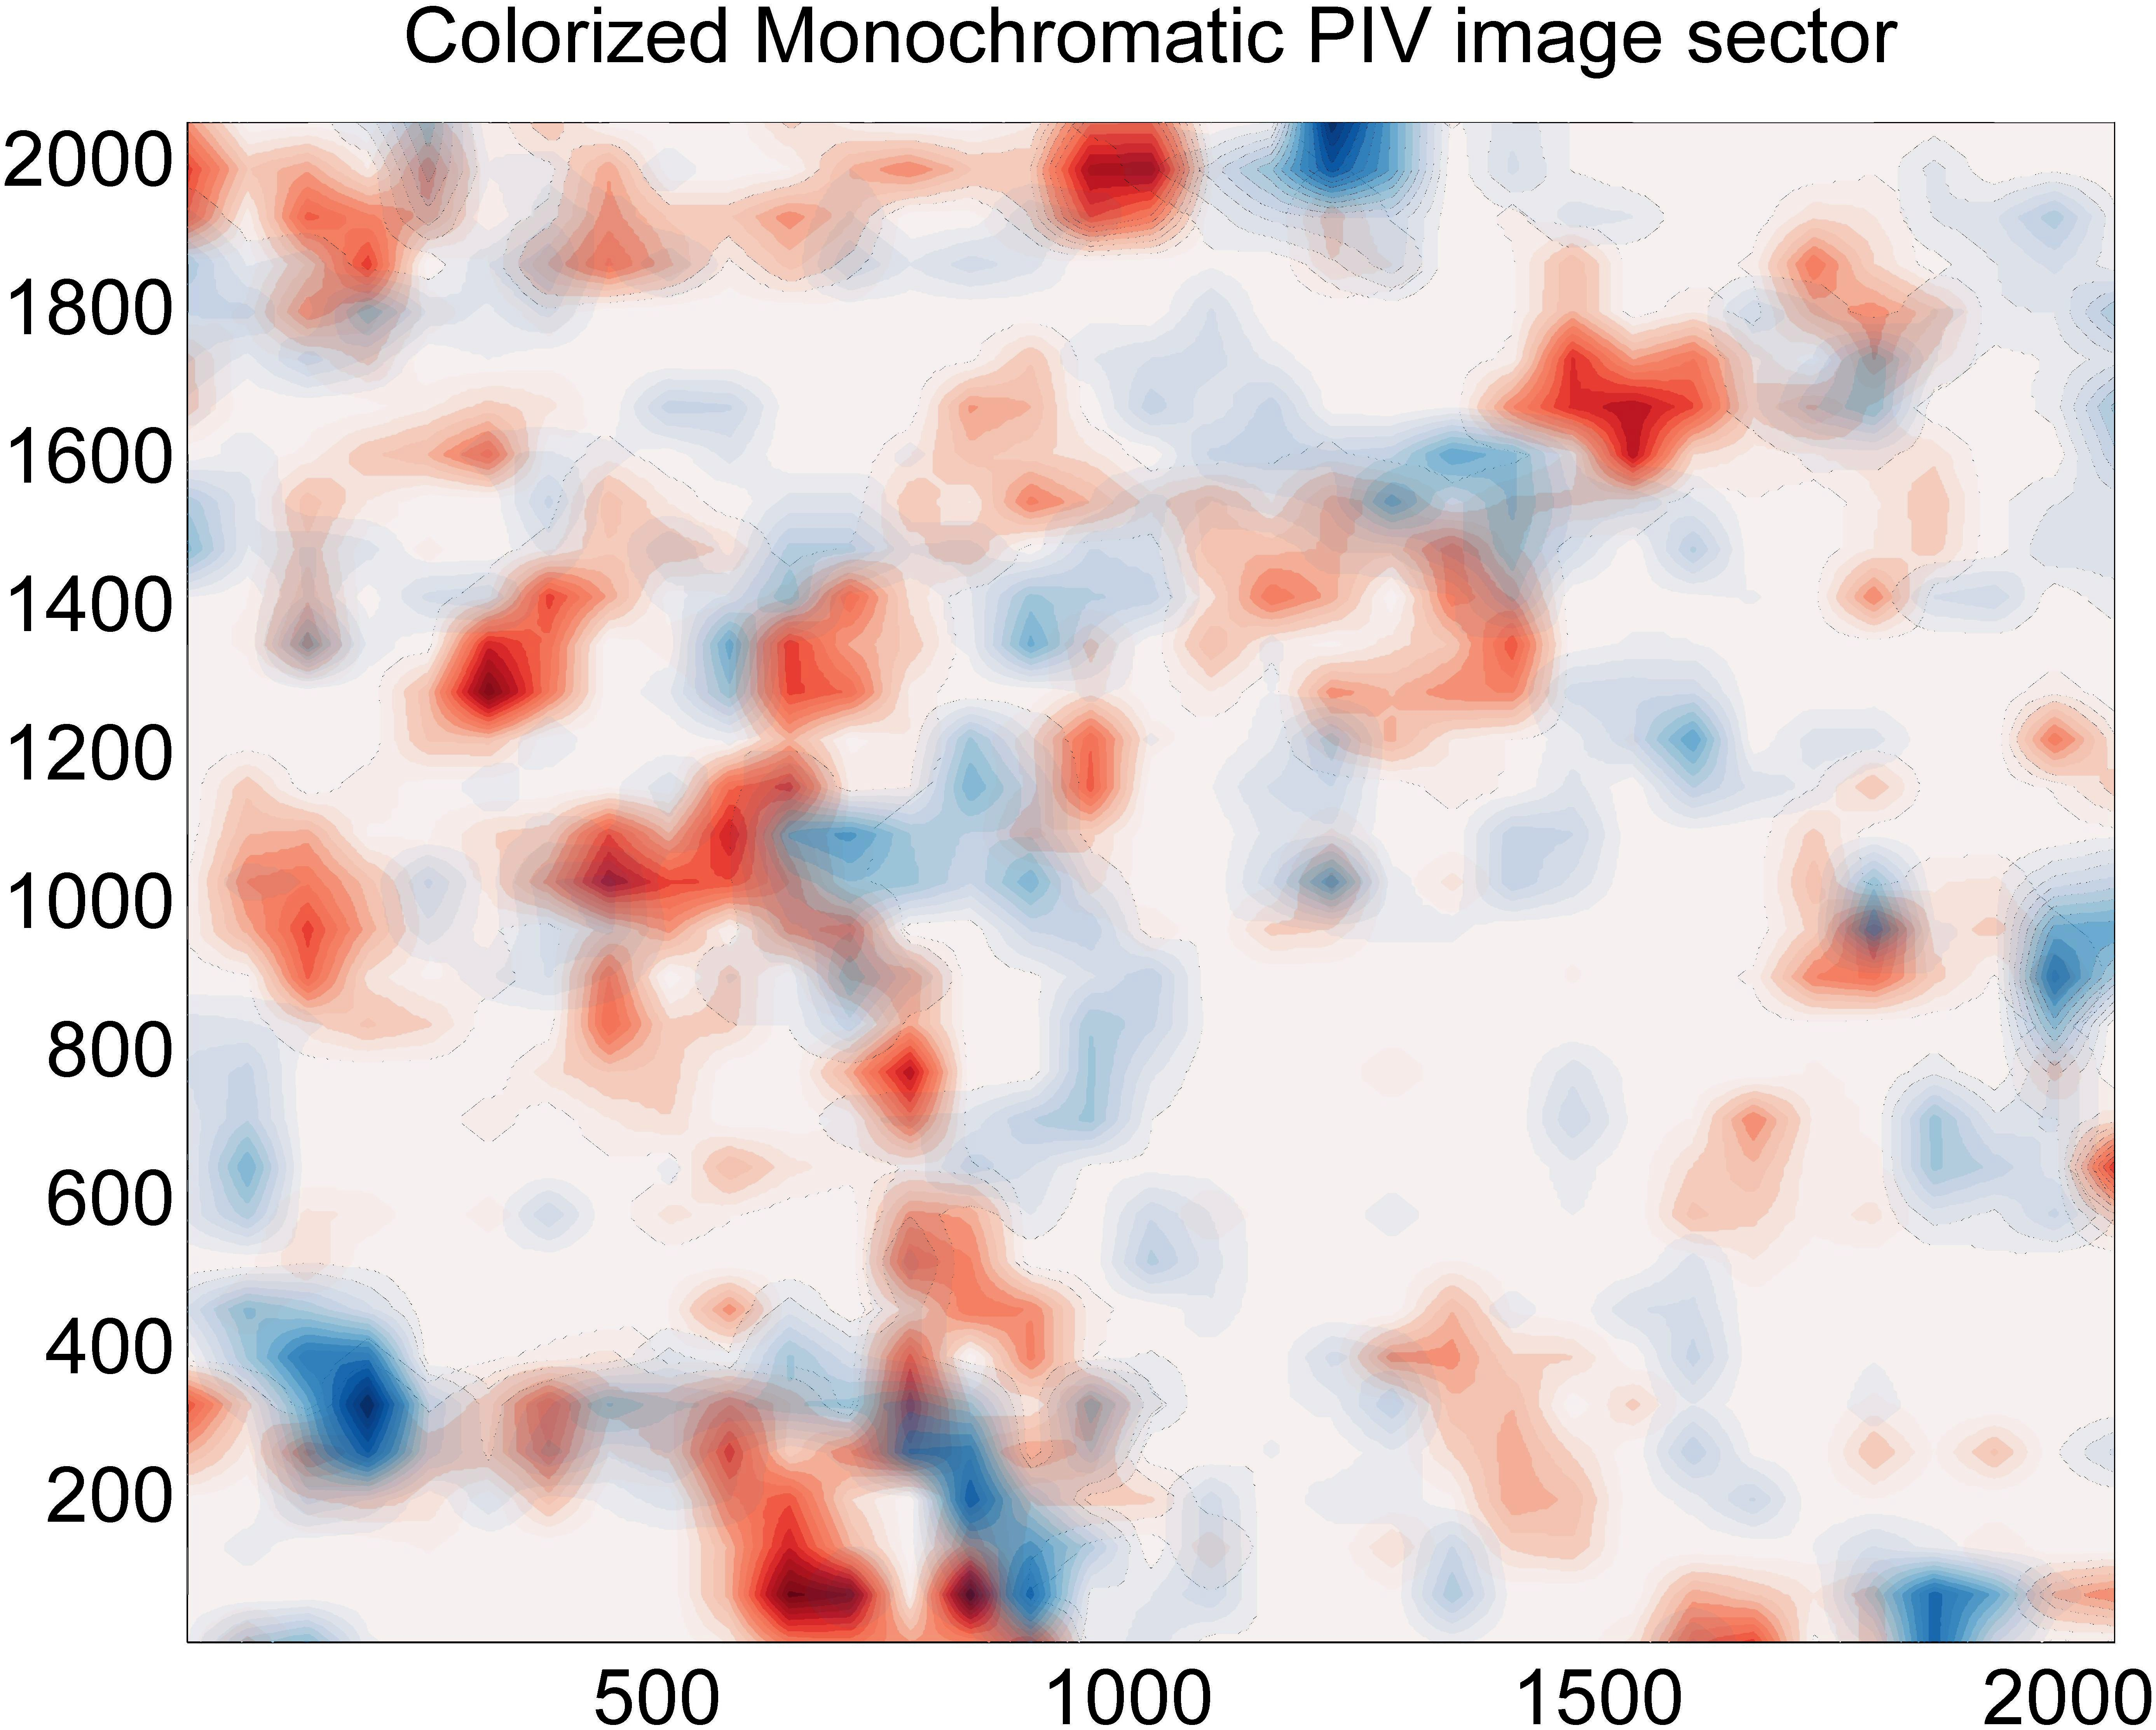
\includegraphics[width=.9\linewidth]{figs/piv_method/pive-fig_order6}
	\end{subfigure} 
	\begin{subfigure}{.49\textwidth}
		\centering
		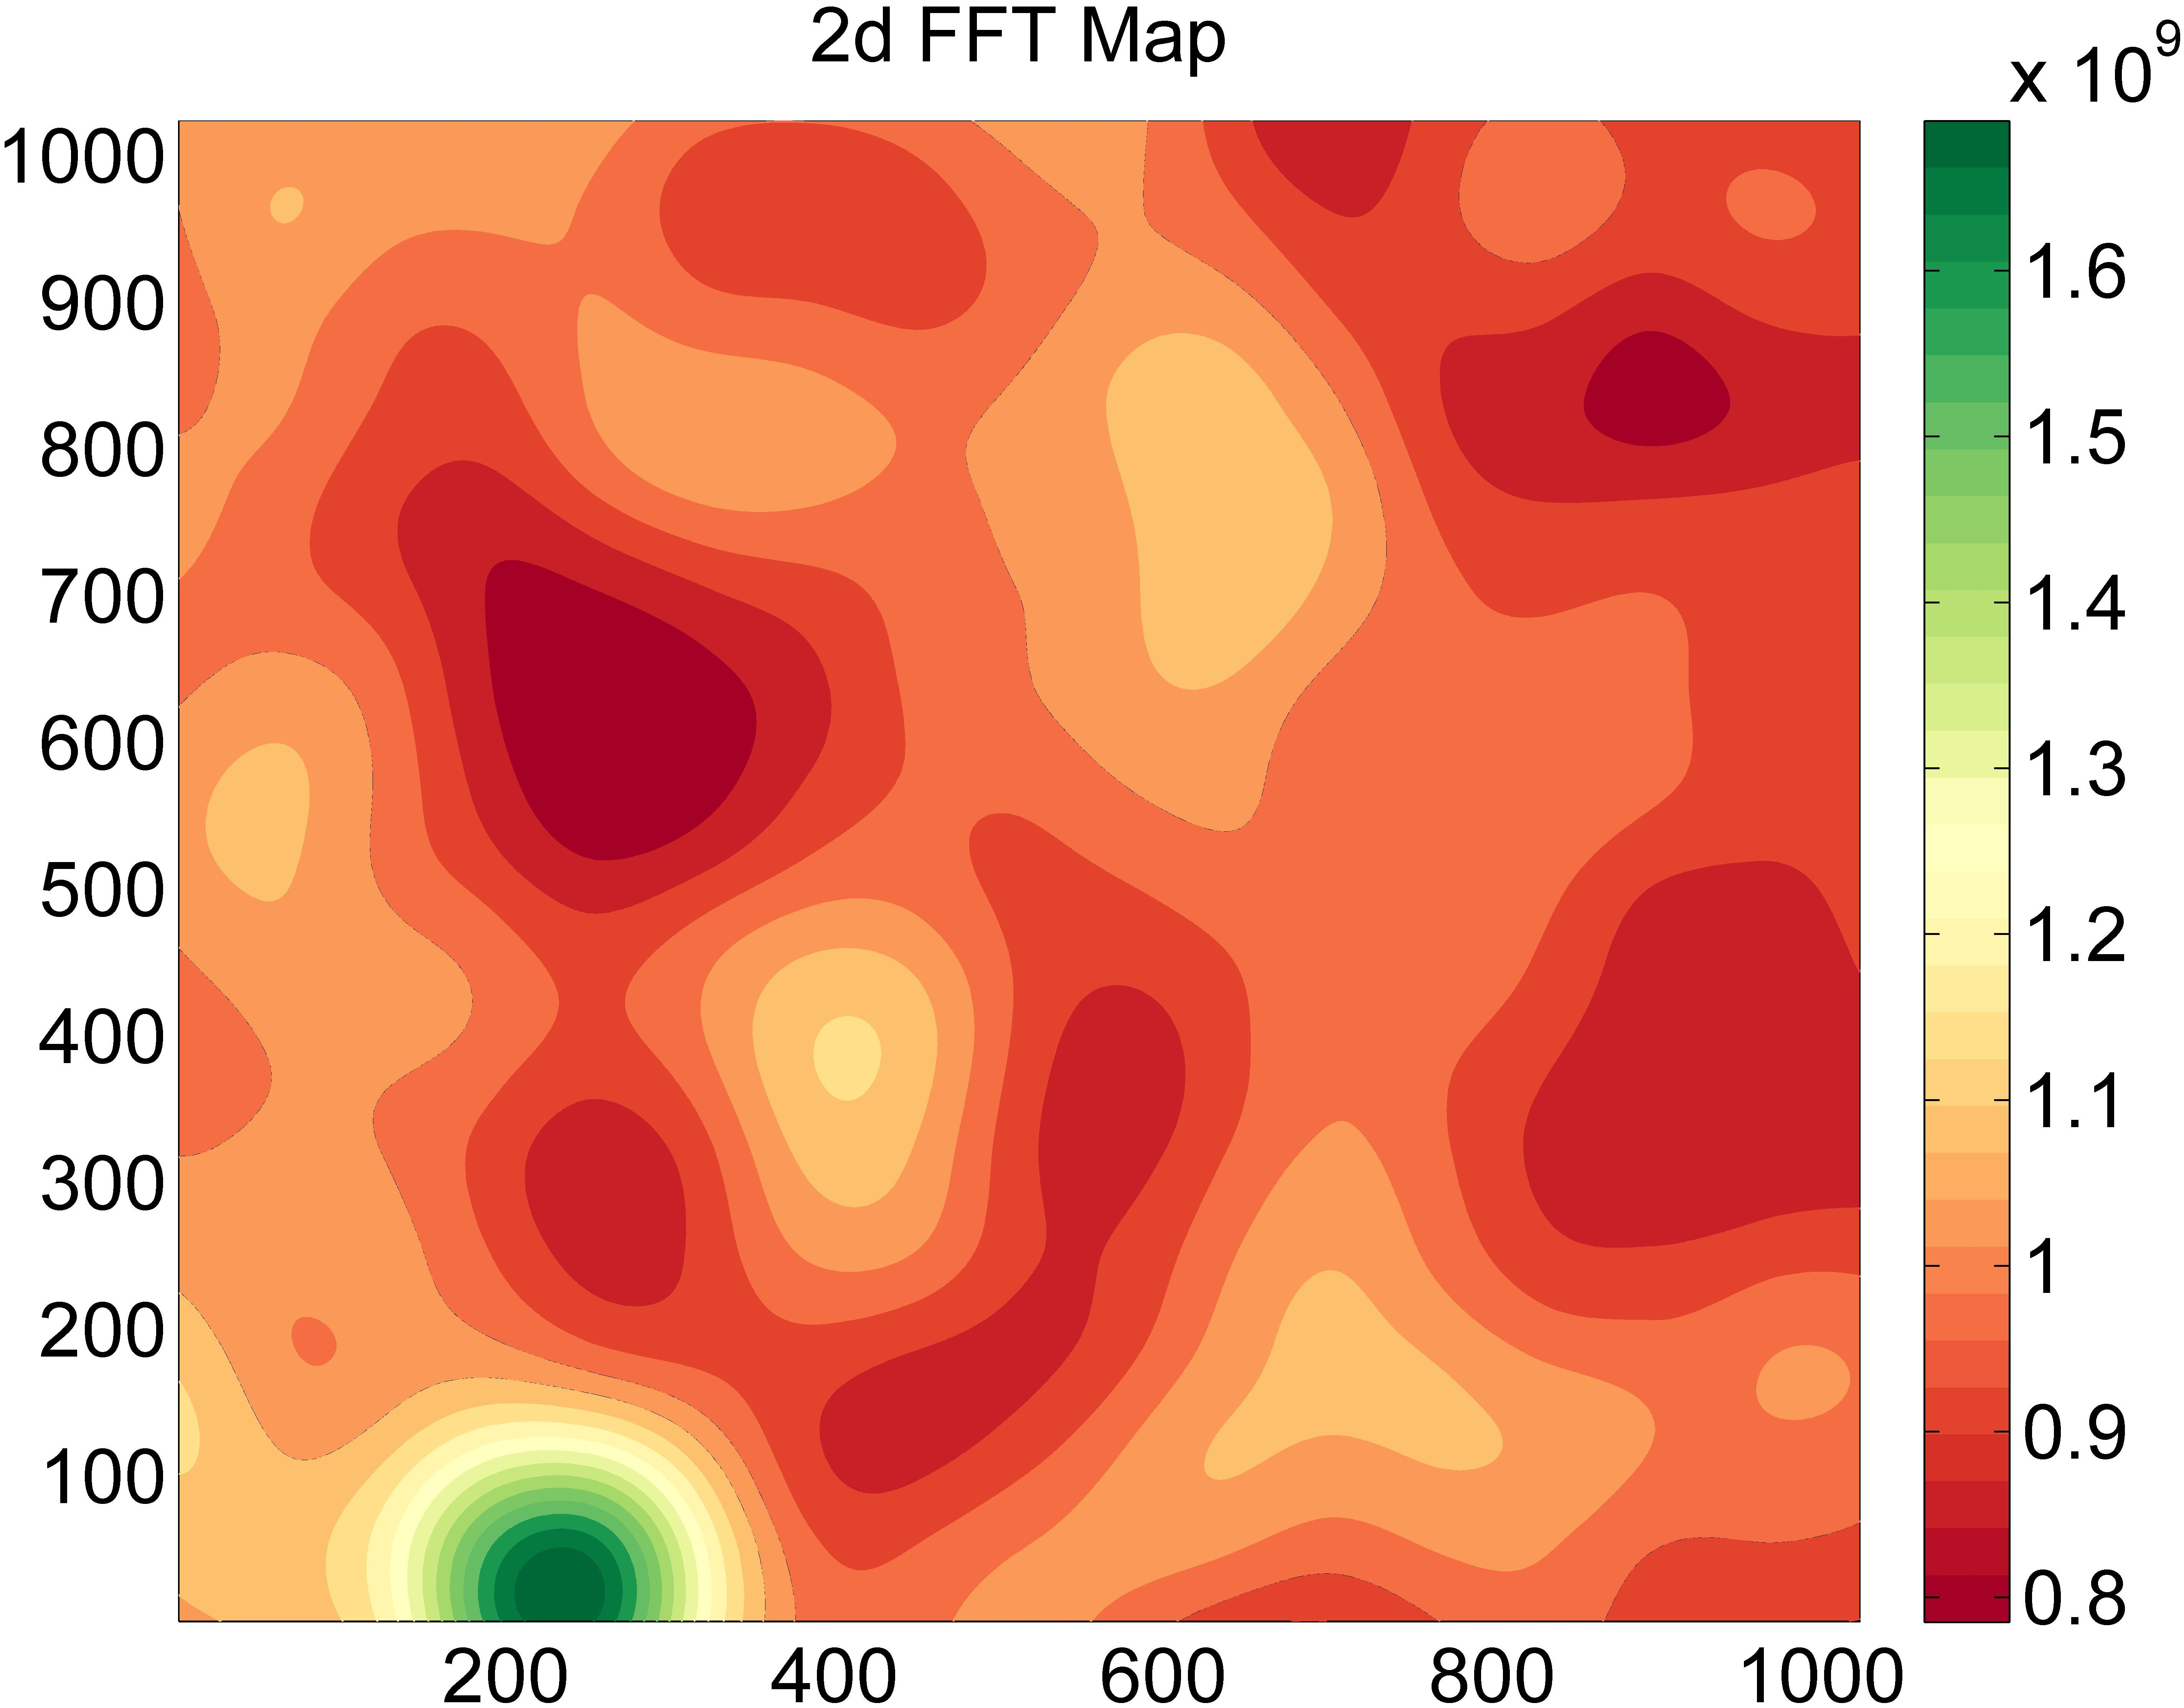
\includegraphics[width=.9\linewidth]{figs/piv_method/pive_fft_order6}
	\end{subfigure}	
	\caption{Overlaid sector snapshots (left) and corresponding correlation 
		map (right), 6th order up sampling.}
	\label{fig:piv_sector_overlay_fft_6up}
\end{figure}

As the sampling method creates a finer mesh, the sub-pixel resolution 
increases. Table \ref{table:piv_upsampling_displacement} shows how the 
displacement error may vary with sampling order.

\begin{table}[H]
\begin{center}
\begin{tabular}{|ccc|}
	\hline
	Order & $x_{disp}$ & $y_{disp}$\\
	\hline
	0 & 4 & 0\\
	1 & 3.5 & 0.5\\
	2 & 3.75 & 0.25\\
	3 & 3.625 & 0.25\\
	4 & 3.625 & 0.3125\\
	5 & 3.625 & 0.3125\\
	6 & 3.6406 & 0.2969\\
	7 & 3.6406 & 0.2969\\
	\hline
\end{tabular}
\caption{Pixel displacements by up sampling order.}
\label{table:piv_upsampling_displacement}
\end{center}
\end{table}


While the above analysis demonstrates the mathematical motivation behind up 
sampling images before performing a Fourier transform for measuring particle 
displacement, it does not adequately describe the total uncertainty in 
measurements made with particle image velocimetry. The uncertainty associated 
with measurements made with PIV are dependent upon the geometry of the specific 
optical setup used to take the data.

In stereo PIV, Equations \ref{eq:piv_to_real1} to \ref{eq:piv_to_real4} the 
derivative terms which relate displacements in the image plane to displacements 
in the real plane are not constant throughout the entire interrogation plane, 
but are functions of the pixels position. These functions can be determined by 
measurement of a calibration target, which has a pattern of dots of known 
position \cite{fouras2007}. The known position of these calibration points can 
be used to compute the nine coefficients for four functions of the form in 
Equation \ref{eq:calibration_equation}. There exists a separate set of nine 
coefficients for the left and right camera, in the $X$ and $Y$ directions.

\begin{equation}
	\begin{multlined}
	X_{mm} =  [A + B(X_{px}) + C(Y_{px}) + D(Z_{mm}) + E(X_{px}^2) + \\
	F(Y_{px}^2) + G(X_{px}Z_{mm}) + H(Y_{px}Z_{mm}) + J(X_{px}Y_{px})]
	\end{multlined}
	\label{eq:calibration_equation}
\end{equation}
\newline
\noindent
where $X_{mm}$ is the position in $mm$, $[A, B, C, D, E, F, G, H, J]$ 
represents the entire set of nine coefficients, $X_{px} and Y_{px}$ are the 
pixel positions in the $X$ and $Y$ directions of the camera plane 
respectively. And $Z_{mm}$ is the actual position in the $Z$ direction. The 
$Z_{mm}$ position of all particles is assumed to be zero in the first image, 
and is determined relative to its starting position by root mean squared of 
the solutions to Equations \ref{eq:piv_to_real1} to \ref{eq:piv_to_real4}.
For simple optical setups, this approach also accounts for distortion due to 
variations in magnification \cite{soloff1997, willert1997}.

\subsection{Uncertainty in PIV}

Understanding the uncertainty in a PIV measurement can be accomplished with 
analysis of the PIV optical geometry \cite{lawson1997b}. Alternatively, Monte 
Carlo techniques for evaluating PIV uncertainty can be used by creating 
artificial image pairs with simulated particle displacements and passing them 
through the PIV processing chain. In PIV, each camera will have a set of 
equations which allow pixel coordinates to be mapped to coordinates of the 
interrogation plane. Particles are simulated with random coordinates within the 
views of both cameras in the interrogation plane, then mapped onto the 
coordinate system of both cameras. The intensity of each pixel can be 
determined by summing the intensity function of every randomly generated 
particle as in \cite{adeyinka2005,fouras2007}.






\fi
%=========================================================================
\iftrue		% set to \iftrue to print to the next \fi, \iffalse not to
\chapter{Experiment Setup}
A complete particle image velocimetry system was installed in the ODU low speed 
wind tunnel and employed to measure three-dimensional velocity fields produced 
by an axial vortex at multiple nominal velocities $V_{nom}$ and multiple 
interrogation planes. The interrogation planes were defined by their 
distance downstream of trailing edges of the bi-wing the vortex generator 
$I_Z$. Nominal wind tunnel velocity was varied from 15$m/s$ to 33$m/s$, 
sampling 10 distinct velocities in increments of 2$m/s$. The interrogation 
plane was moved at irregular intervals from 546$mm$ to 1016$mm$, 5.4 to 10 
chord lengths, as shown in Table \ref{table:test_matrix_table}. This chapter 
discuss details of the experimental setup used to produce these datasets, 
including wind tunnel control, vortex generator setup, PIV system calibration, 
data acquisition, data processing, and data quality control.
\renewcommand\baselinestretch{1.3}\selectfont
\begin{table}[H]
\begin{center}
\begin{tabular}{|ccc||ccc||ccc|}
	\hline
	Run & $I_Z$  & $V_{nom}$ & Run & $I_Z$  & $V_{nom}$ & Run & $I_Z$  & $V_{nom}$\\
	ID & ($mm$) & ($m/s$) & ID & ($mm$) & ($m/s$) & ID & ($mm$) & ($m/s$)\\
	\hline
	1 & 546 & 15 & 31 & 863 & 15 & 61 & 1016 & 15\\
	2 & 546 & 17 & 32 & 863 & 17 & 62 & 1016 & 17\\
	3 & 546 & 19 & 33 & 863 & 19 & 63 & 1016 & 19\\
	4 & 546 & 21 & 34 & 863 & 21 & 64 & 1016 & 21\\
	5 & 546 & 23 & 35 & 863 & 23 & 65 & 1016 & 23\\
	6 & 546 & 25 & 36 & 863 & 25 & 66 & 1016 & 25\\
	7 & 546 & 27 & 37 & 863 & 27 & 67 & 1016 & 27\\
	8 & 546 & 29 & 38 & 863 & 29 & 68 & 1016 & 29\\
	9 & 546 & 31 & 39 & 863 & 31 & 69 & 1016 & 31\\
	10 & 546 & 33 & 40 & 863 & 33 & 70 & 1016 & 33\\
	11 & 708 & 15 & 41 & 914 & 15 &   &   &  \\
	12 & 708 & 17 & 42 & 914 & 17 &   &   &  \\
	13 & 708 & 19 & 43 & 914 & 19 &   &   &  \\
	14 & 708 & 21 & 44 & 914 & 21 &   &   &  \\
	15 & 708 & 23 & 45 & 914 & 23 &   &   &  \\
	16 & 708 & 25 & 46 & 914 & 25 &   &   &  \\
	17 & 708 & 27 & 47 & 914 & 27 &   &   &  \\
	18 & 708 & 29 & 48 & 914 & 29 &   &   &  \\
	19 & 708 & 31 & 49 & 914 & 31 &   &   &  \\
	20 & 708 & 33 & 50 & 914 & 33 &   &   &  \\
	21 & 787 & 15 & 51 & 965 & 15 &   &   &  \\
	22 & 787 & 17 & 52 & 965 & 17 &   &   &  \\
	23 & 787 & 19 & 53 & 965 & 19 &   &   &  \\
	24 & 787 & 21 & 54 & 965 & 21 &   &   &  \\
	25 & 787 & 23 & 55 & 965 & 23 &   &   &  \\
	26 & 787 & 25 & 56 & 965 & 25 &   &   &  \\
	27 & 787 & 27 & 57 & 965 & 27 &   &   &  \\
	28 & 787 & 29 & 58 & 965 & 29 &   &   &  \\
	29 & 787 & 31 & 59 & 965 & 31 &   &   &  \\
	30 & 787 & 33 & 60 & 965 & 33 &   &   &  \\
	\hline
\end{tabular}
\caption{Experimental conditions for all 70 experiments}
\label{table:test_matrix_table}
\end{center}
\end{table}
\renewcommand\baselinestretch{2}\selectfont


\section{Low Speed Wind Tunnel}

The Old Dominion University low 
speed wind tunnel (LSWT) was outfitted with a bi-wing axial vortex generator. 
The tunnel has a large test section measuring 2.134$m$ wide by 2.438$m$ 
tall and a smaller, higher speed test section measuring 1.219$m$ wide by 
0.911$m$ tall (3 x 4 feet). The 
wind tunnel air is propelled with a fan on a frequency controlled 125 
horsepower motor. 
Flow velocity was manipulated directly by manually controlling
voltage supplied to the controller. 
The small test section, used in the present experimental investigation, has a 
total length of 2.438$m$, and the vertically mounted vortex generator 
spanned the 0.911$m$ height of the test section and was 
mounted 0.610$m$ from the end of the flow contraction section, leaving 1.829$m$ 
downstream for the axial 
vortex to develop. The high speed test section has a functional free stream 
velocity range between 12 and 55  $m/s$ or between 35 and 120 $mph$.

\begin{figure}[H]
\centering
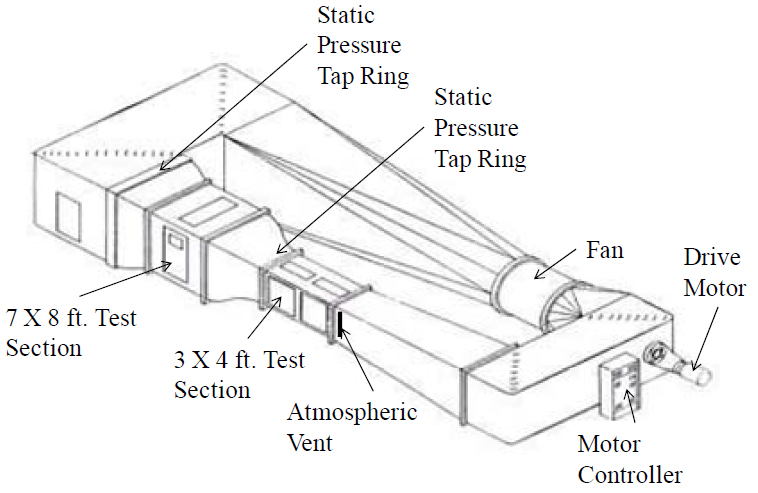
\includegraphics[width=5in]{figs/setup/odulswt_diagram}
\caption{ODU Low speed wind tunnel.}
\label{fig:odulswt}
\end{figure}

The entire interior of the test section was vacant and unobstructed beyond the 
vortex generator. 
No internal traverse systems or structures 
were present during PIV data acquisition unless otherwise indicated. Tunnel 
velocity was determined by direct measurement of dynamic pressure ($q$), 
barometric pressure, and temperature, which 
are monitored and controlled by the tunnel control PC. A functional schematic 
of the LSWT PC-based tunnel control system is shown in Figure 
\ref{fig:control_diagram}.

\begin{figure}[H]
\centering
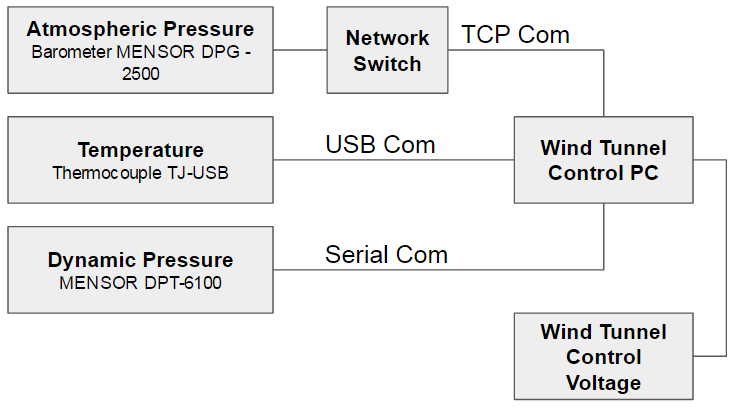
\includegraphics[width=4in]{figs/setup/odulswt_control}
\caption{Schematic diagram of systems under wind tunnel PC control.}
\label{fig:control_diagram}
\end{figure}



\section{Vortex Generator}

It is desirable to enhance understanding of 
trailing axial vortices generated by aircraft wingtips.
While naturally occurring axial vortices occur in unpredictable and non-uniform 
environments, this experimental investigation required a repeatable axial 
vortex.  Small-scale aircraft axial wake vortices can be generated in an 
enclosed wind tunnel environment with a single wingtip, but the downwash 
behavior resulting from a lift-generating wingtip vortex causes the rotational 
axis to curve and become distorted by the walls of the wind tunnel and
test section. A bi-wing vortex generator, as pictured in Figures 
\ref{fig:vortex_gen} and \ref{fig:vortex_design}, was designed and constructed 
by undergraduate student researchers to generate a vortex with two opposing 
wings, producing a single vortex, absent any downwash effects \cite{davis2012}. 
The vortex generator employed two symmetric NACA-0012
airfoils with chord lengths of 101.6$mm$, manufactured from foam casts. Both 
airfoils were attached 
to a 25.4$mm$ diameter cylindrical center body with hemispherical forward and 
aft end caps. While the vortex generator could have allowed angles-of-attack 
adjustments, the precision with which the adjustments could be made was 
considered to be inadequate for producing repeatable results, so the wings were 
locked at angles-of-attack of $\pm$8 degrees.

\vspace{32pt}
\begin{figure}[H]
\centering
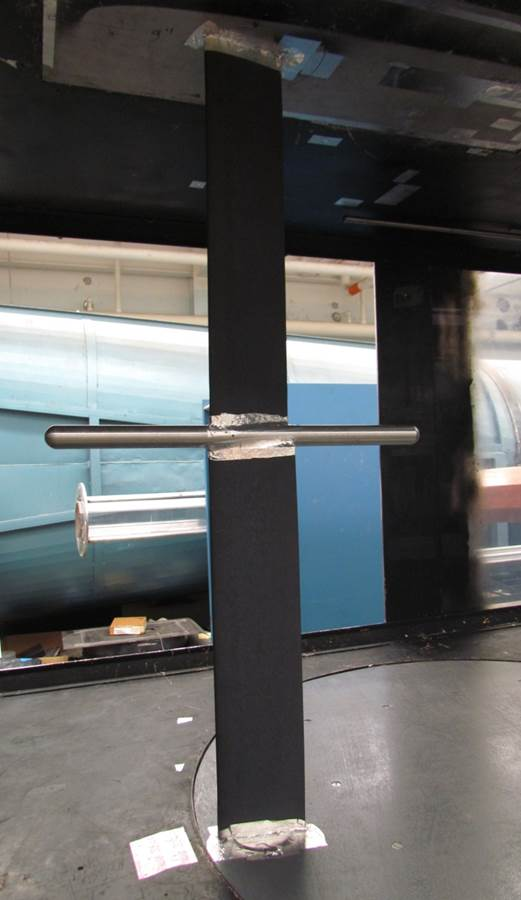
\includegraphics[width=4in]{figs/setup/vortex_generator/picture}
\caption{Picture of the vortex generator set up in the ODU LSWT.}
\label{fig:vortex_gen}
\end{figure}

\begin{figure}[H]
\centering
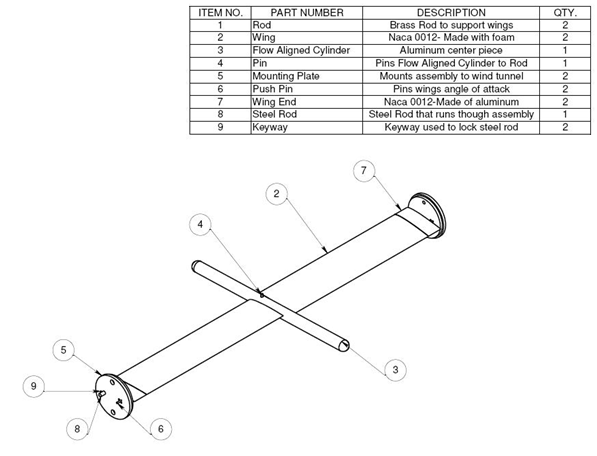
\includegraphics[width=5.75in]{figs/setup/vortex_generator/design}
\caption{CAD design of the vortex generator used in this study.}
\label{fig:vortex_design}
\end{figure}



\section{PIV Overview}

The present study uses a stereo PIV system which resolves three dimensional 
near-instantaneous velocity vectors gridded on a two dimensional cross section 
of flow. The cameras are capable of taking two images just a few microseconds 
apart. Determining velocity vectors requires two images just a few 
microseconds apart, but pairs of images can be taken at greater time intervals. 
The PIV method used in this study utilizes a "frame-straddling" technique that 
spaces the time interval between two laser pulses so that the camera sensor 
arrays receive the first laser illuminated image data as near as possible to 
the closing of the shutter, followed by a second laser illuminated image as 
close as possible to the beginning of the second shutter opening. This 
technique allows both cameras to capture image sequence pairs simultaneously, 
spaced 25 to 50 microseconds apart. This can be repeated once every second, 
resulting in a true velocity sampling frequency of 1 Hz.

\subsection{Seeding the Flow}

Appropriate particle seeding density and time between straddled frames is the
subject of continued study, and is difficult to predict \textit{a priori}. 
Complete coverage of a two dimensional vector field is highly dependent upon 
uniform optimal particle density conditions which are difficult to obtain, and 
maintain over an extended test interval, due to seed-particle accumulation. For 
stereo PIV, incomplete data in either of the two dimensional vector 
sets from either camera at a given spatial location will result in an 
indeterminate vector displacement in the three dimensional vector data. To 
elevate the likelihood that a displacement vector at a given location can be 
properly determined, an additional data refining technique outlined by 
\cite{hart1998} was employed. The Hart method compares correlation maps 
between adjacent vector spots to produce fewer errors than would otherwise be 
produced by completely independent evaluation of each small image sector. In 
instances where two adjacent regions lack a well-defined peak, the Hart method 
emphasizes shared 
peaks in order to reveal a significant correlation that might otherwise have 
been missed. In instances 
where sub optimal seeding conditions exist and a correlation map 
produces a false peak, the Hart method can isolate and eliminate those 
anomalous peaks based on comparison with adjacent sectors \cite{hart1998}. The 
actual process by which the Hart method reduces erroneous vectors is difficult 
to quantify on a case by case basis, but is expected to have a positive effect 
and reduce overall uncertainty in the PIV measurement.


\section{Stereo PIV Data Acquisition}

The low speed wind tunnel was outfitted with a stereo particle image 
velocimetry system which included two cameras that were mounted with a simple 
frame built from 80$mm$x120$mm$ T-slot extruded aluminum with six sliding 
fastener points on the exterior of the wind tunnel, just outside the test 
section on the left and right sides as shown in figure \ref{fig:pivsetup}. 

\begin{figure}[H]
	\centering
	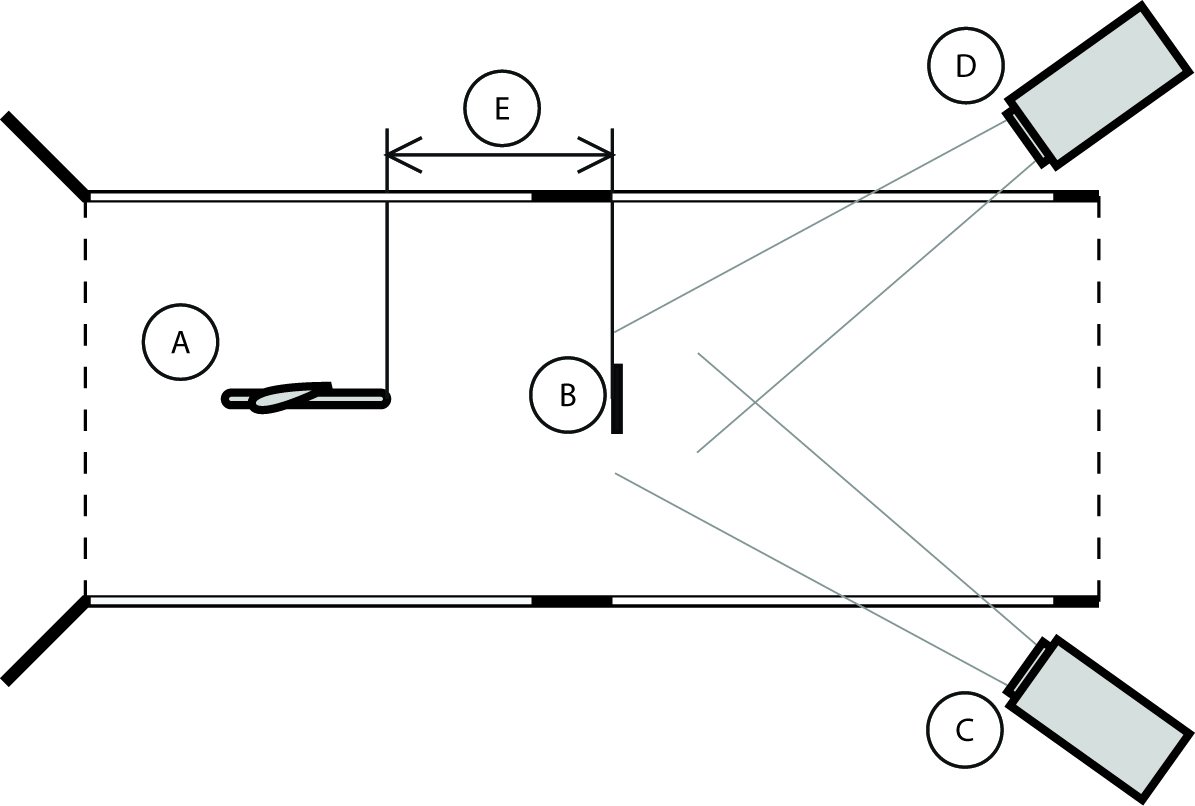
\includegraphics[width=5in]{figs/piv_method/piv_camera_diagram}
	\caption{Top view schematic of PIV camera positions. A-vortex generator, 
	B-PIV 
		calibration target and interrogation plane, C-left camera, D-right 
		camera, E-station distance dimension.}
	\label{fig:pivsetup}
\end{figure}

The roof of the wind tunnel has a long glass window along the center of the 
test section such that an Nd:YAG laser could be mounted to create a vertically 
oriented laser sheet. This laser sheet functioned to illuminate the fluid flow 
perpendicular to the free stream velocity vector as 
shown in Figure \ref{fig:laser_sheet_picture}. In this image, the fluid flow 
has been freshly seeded with a wand to deposit concentrated fog directly 
downstream of the vortex generator to visualize a vortex with a clearly 
defined, smoke free, vortex core. Bright outer lines mark the edges of the 
light curtain. This was initially performed to aid in the alignment of a 
pressure probe (visible in the image) with the vortex core. PIV data was not 
taken with the fog wand or the pressure probe present in the wind tunnel.


The equipment used for this study was a "TSI Stereo Image Velocimeter System", 
which consists of a pair of TSI PIV 13-8 cameras (Figure 
\ref{fig:camera_picture}), a TSI synchronizer and frame 
grabber specific to the cameras (Figures \ref{fig:synchronizer} and 
\ref{fig:synchronizer2}), a New Wave Dual Mini-YAG Laser (Figure 
\ref{fig:laser}), a precision 3-D calibration target for stereo 
PIV camera alignment, and a precision laser traverse system. The particle seed 
was generated by an MDG fog generator (Figure \ref{fig:fog_machine}). The TSI 
INSIGHT\textsuperscript{\textcopyright} software was used 
for data acquisition and image to vector processing.

\begin{figure}[H]
	\centering
	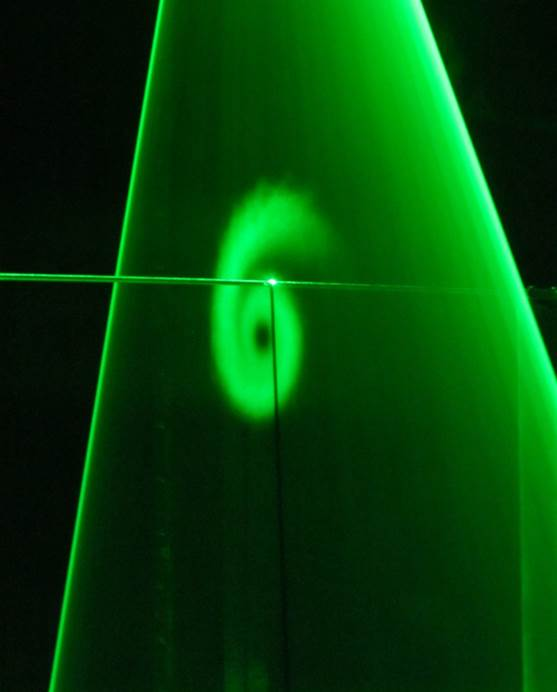
\includegraphics[width=5in]{figs/piv_method/laser_sheet_picture}
	\caption{Picture of a light curtain illuminating a cross section of an 
	axial wake vortex.}
	\label{fig:laser_sheet_picture}
\end{figure}

\begin{figure}[H]
	\centering
	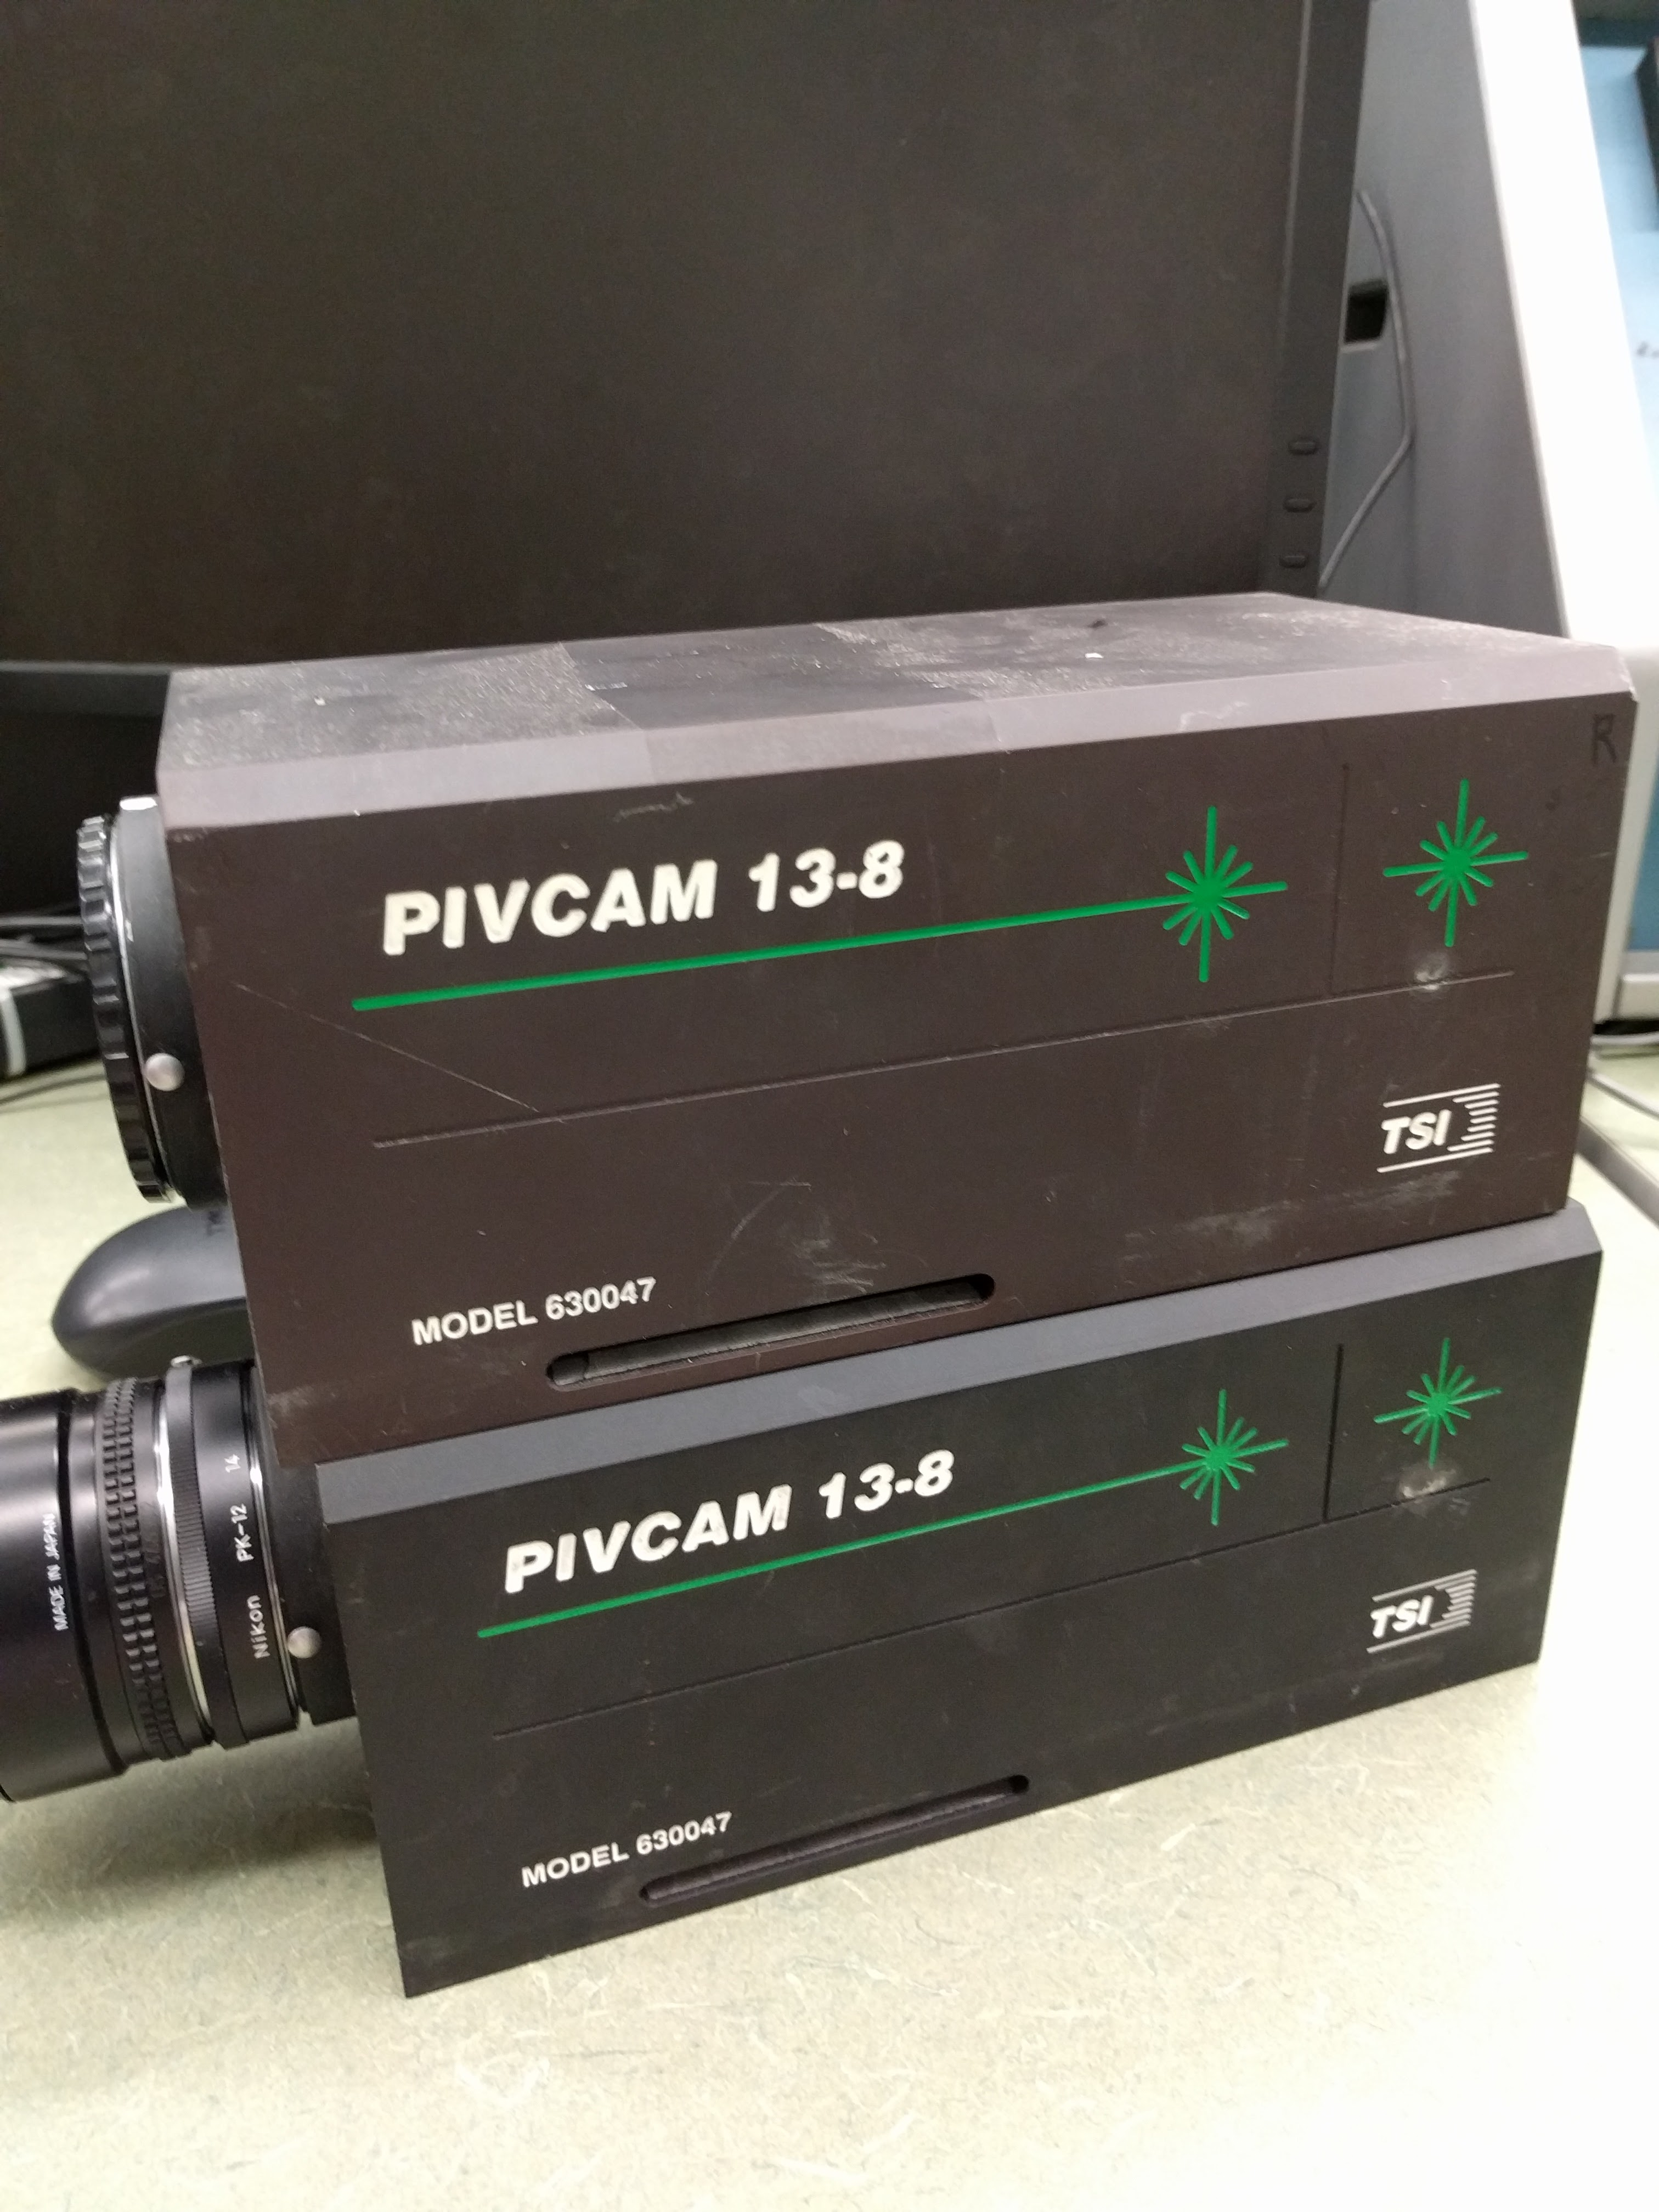
\includegraphics[width=5in]{figs/piv_method/piv_cams}
	\caption{Photograph of two TSI PIV 13-8 cameras. Model 630047}
	\label{fig:camera_picture}
\end{figure}

\begin{figure}[H]
	\centering
	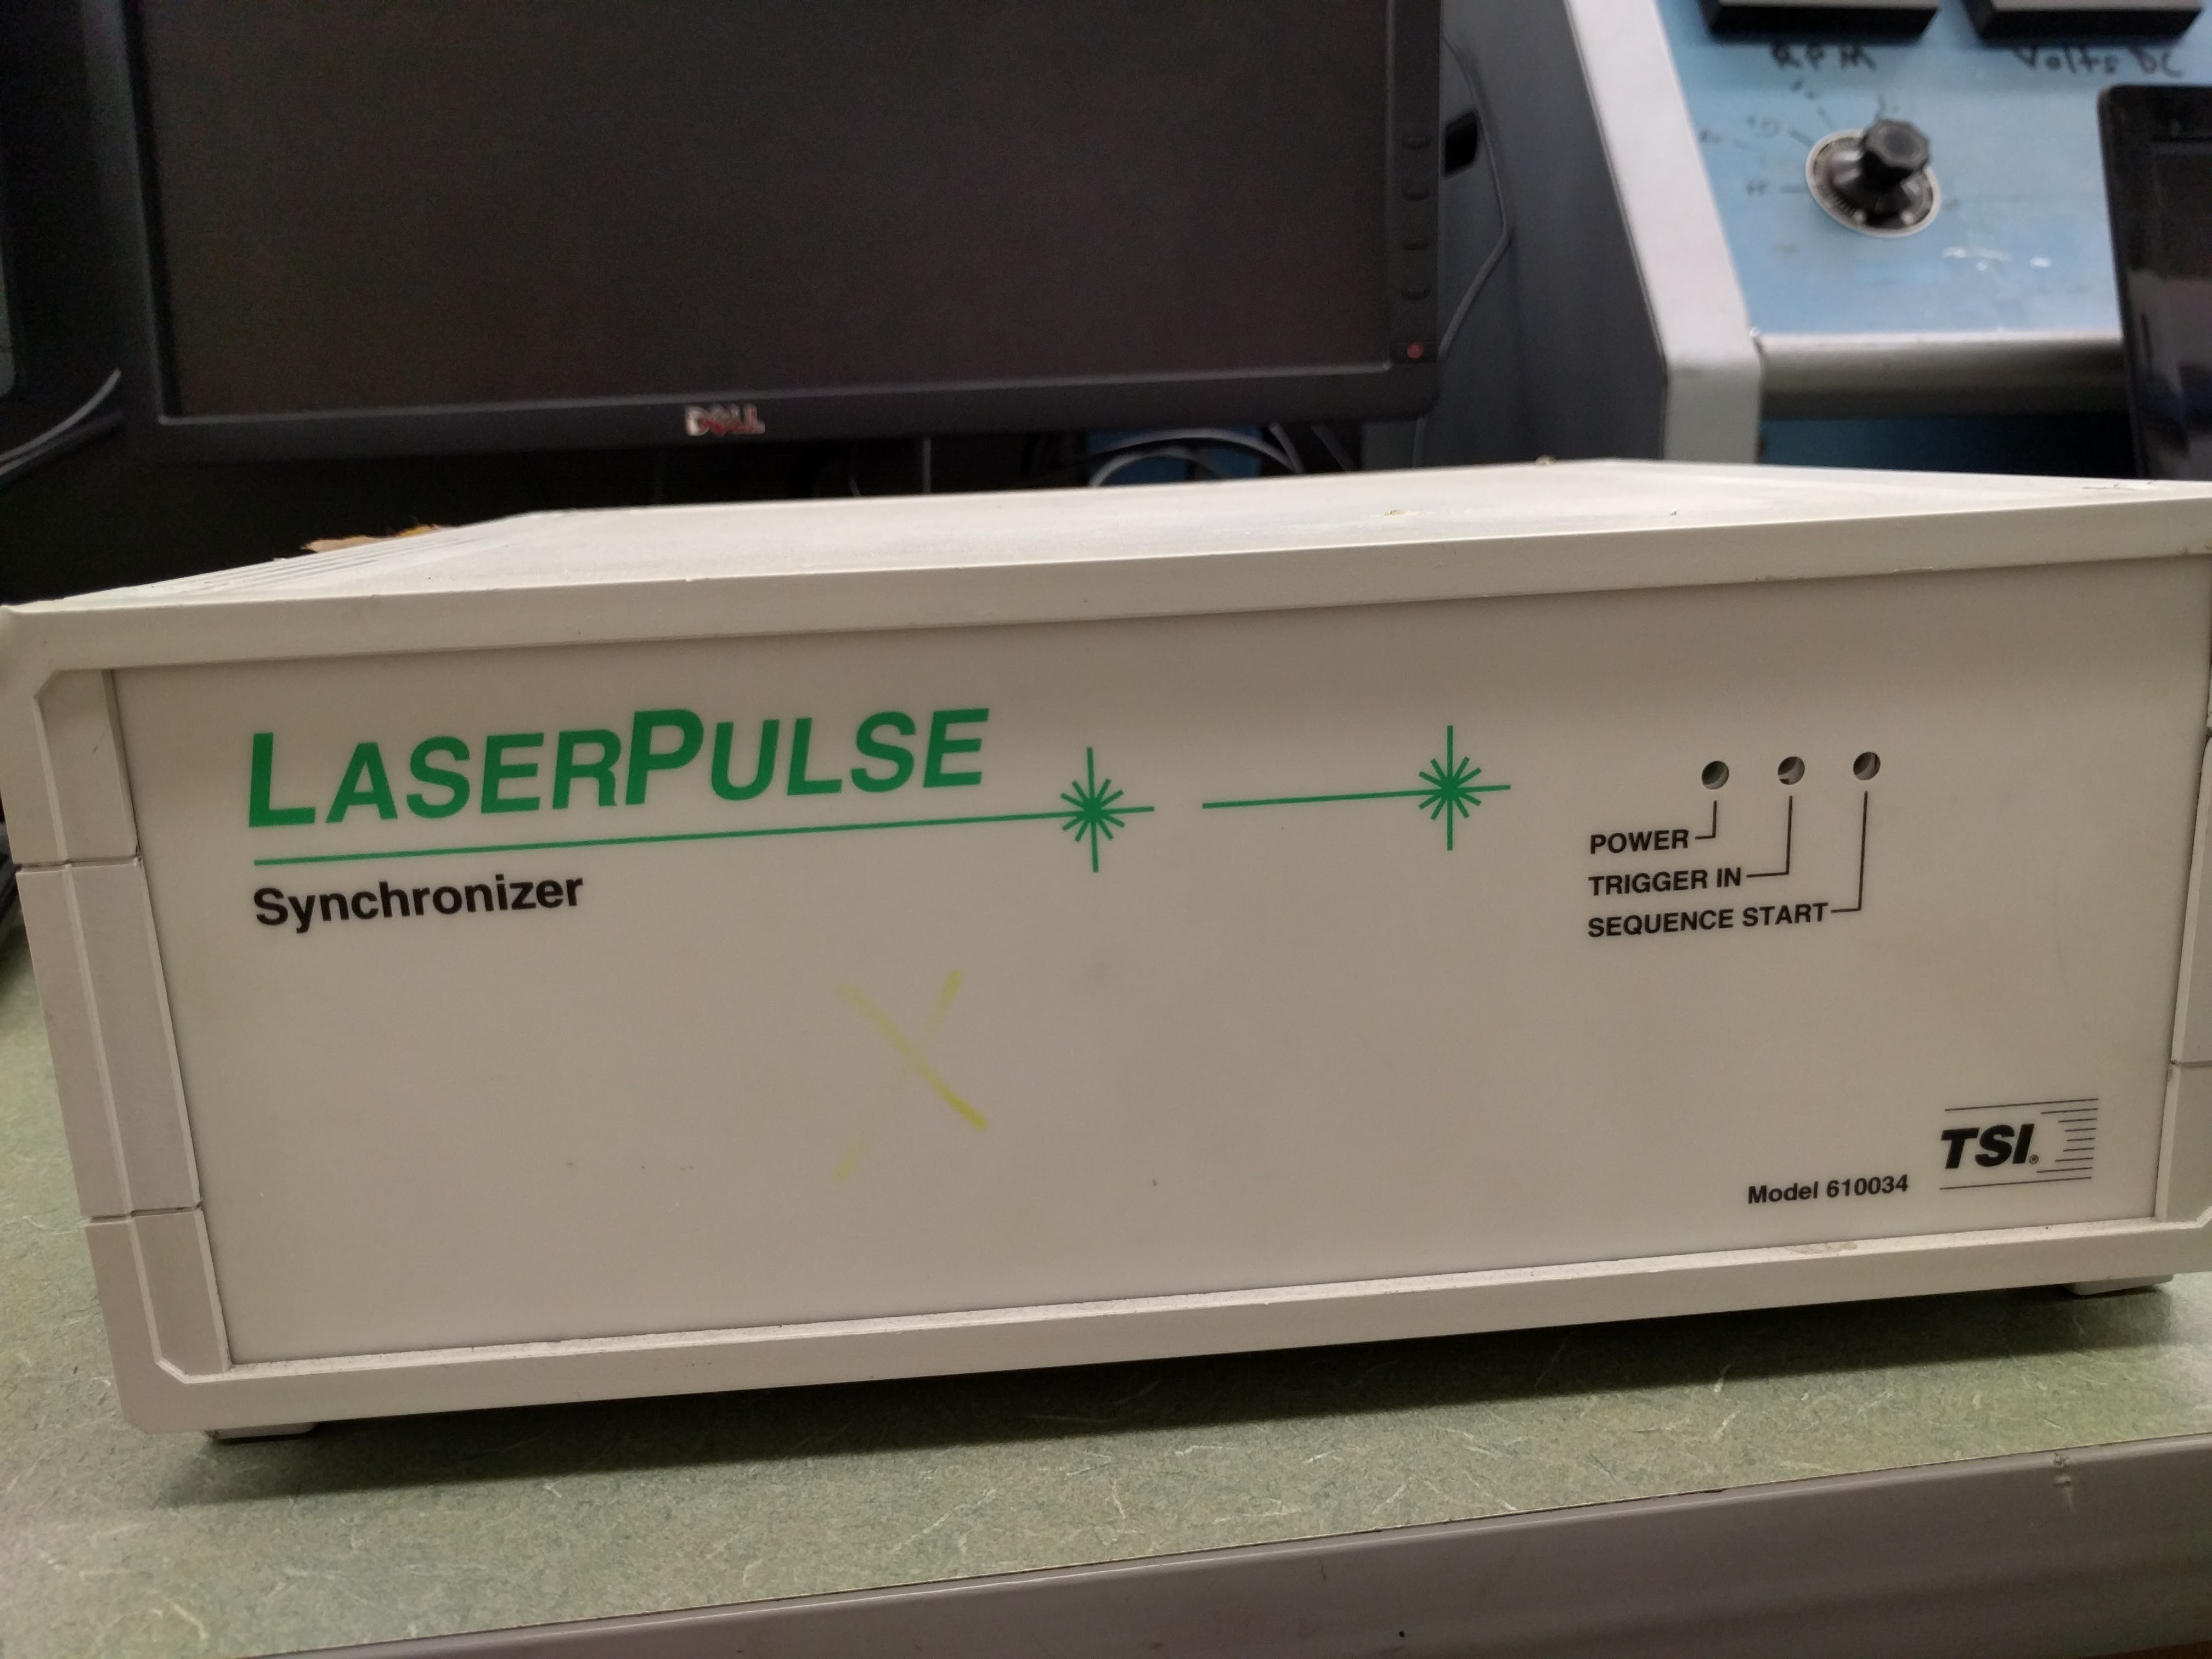
\includegraphics[width=5in]{figs/piv_method/synchronizer}
	\caption{Photograph of LaserPulse synchronizer by TSI. Model 610034}
	\label{fig:synchronizer}
\end{figure}

\begin{figure}[H]
	\centering
	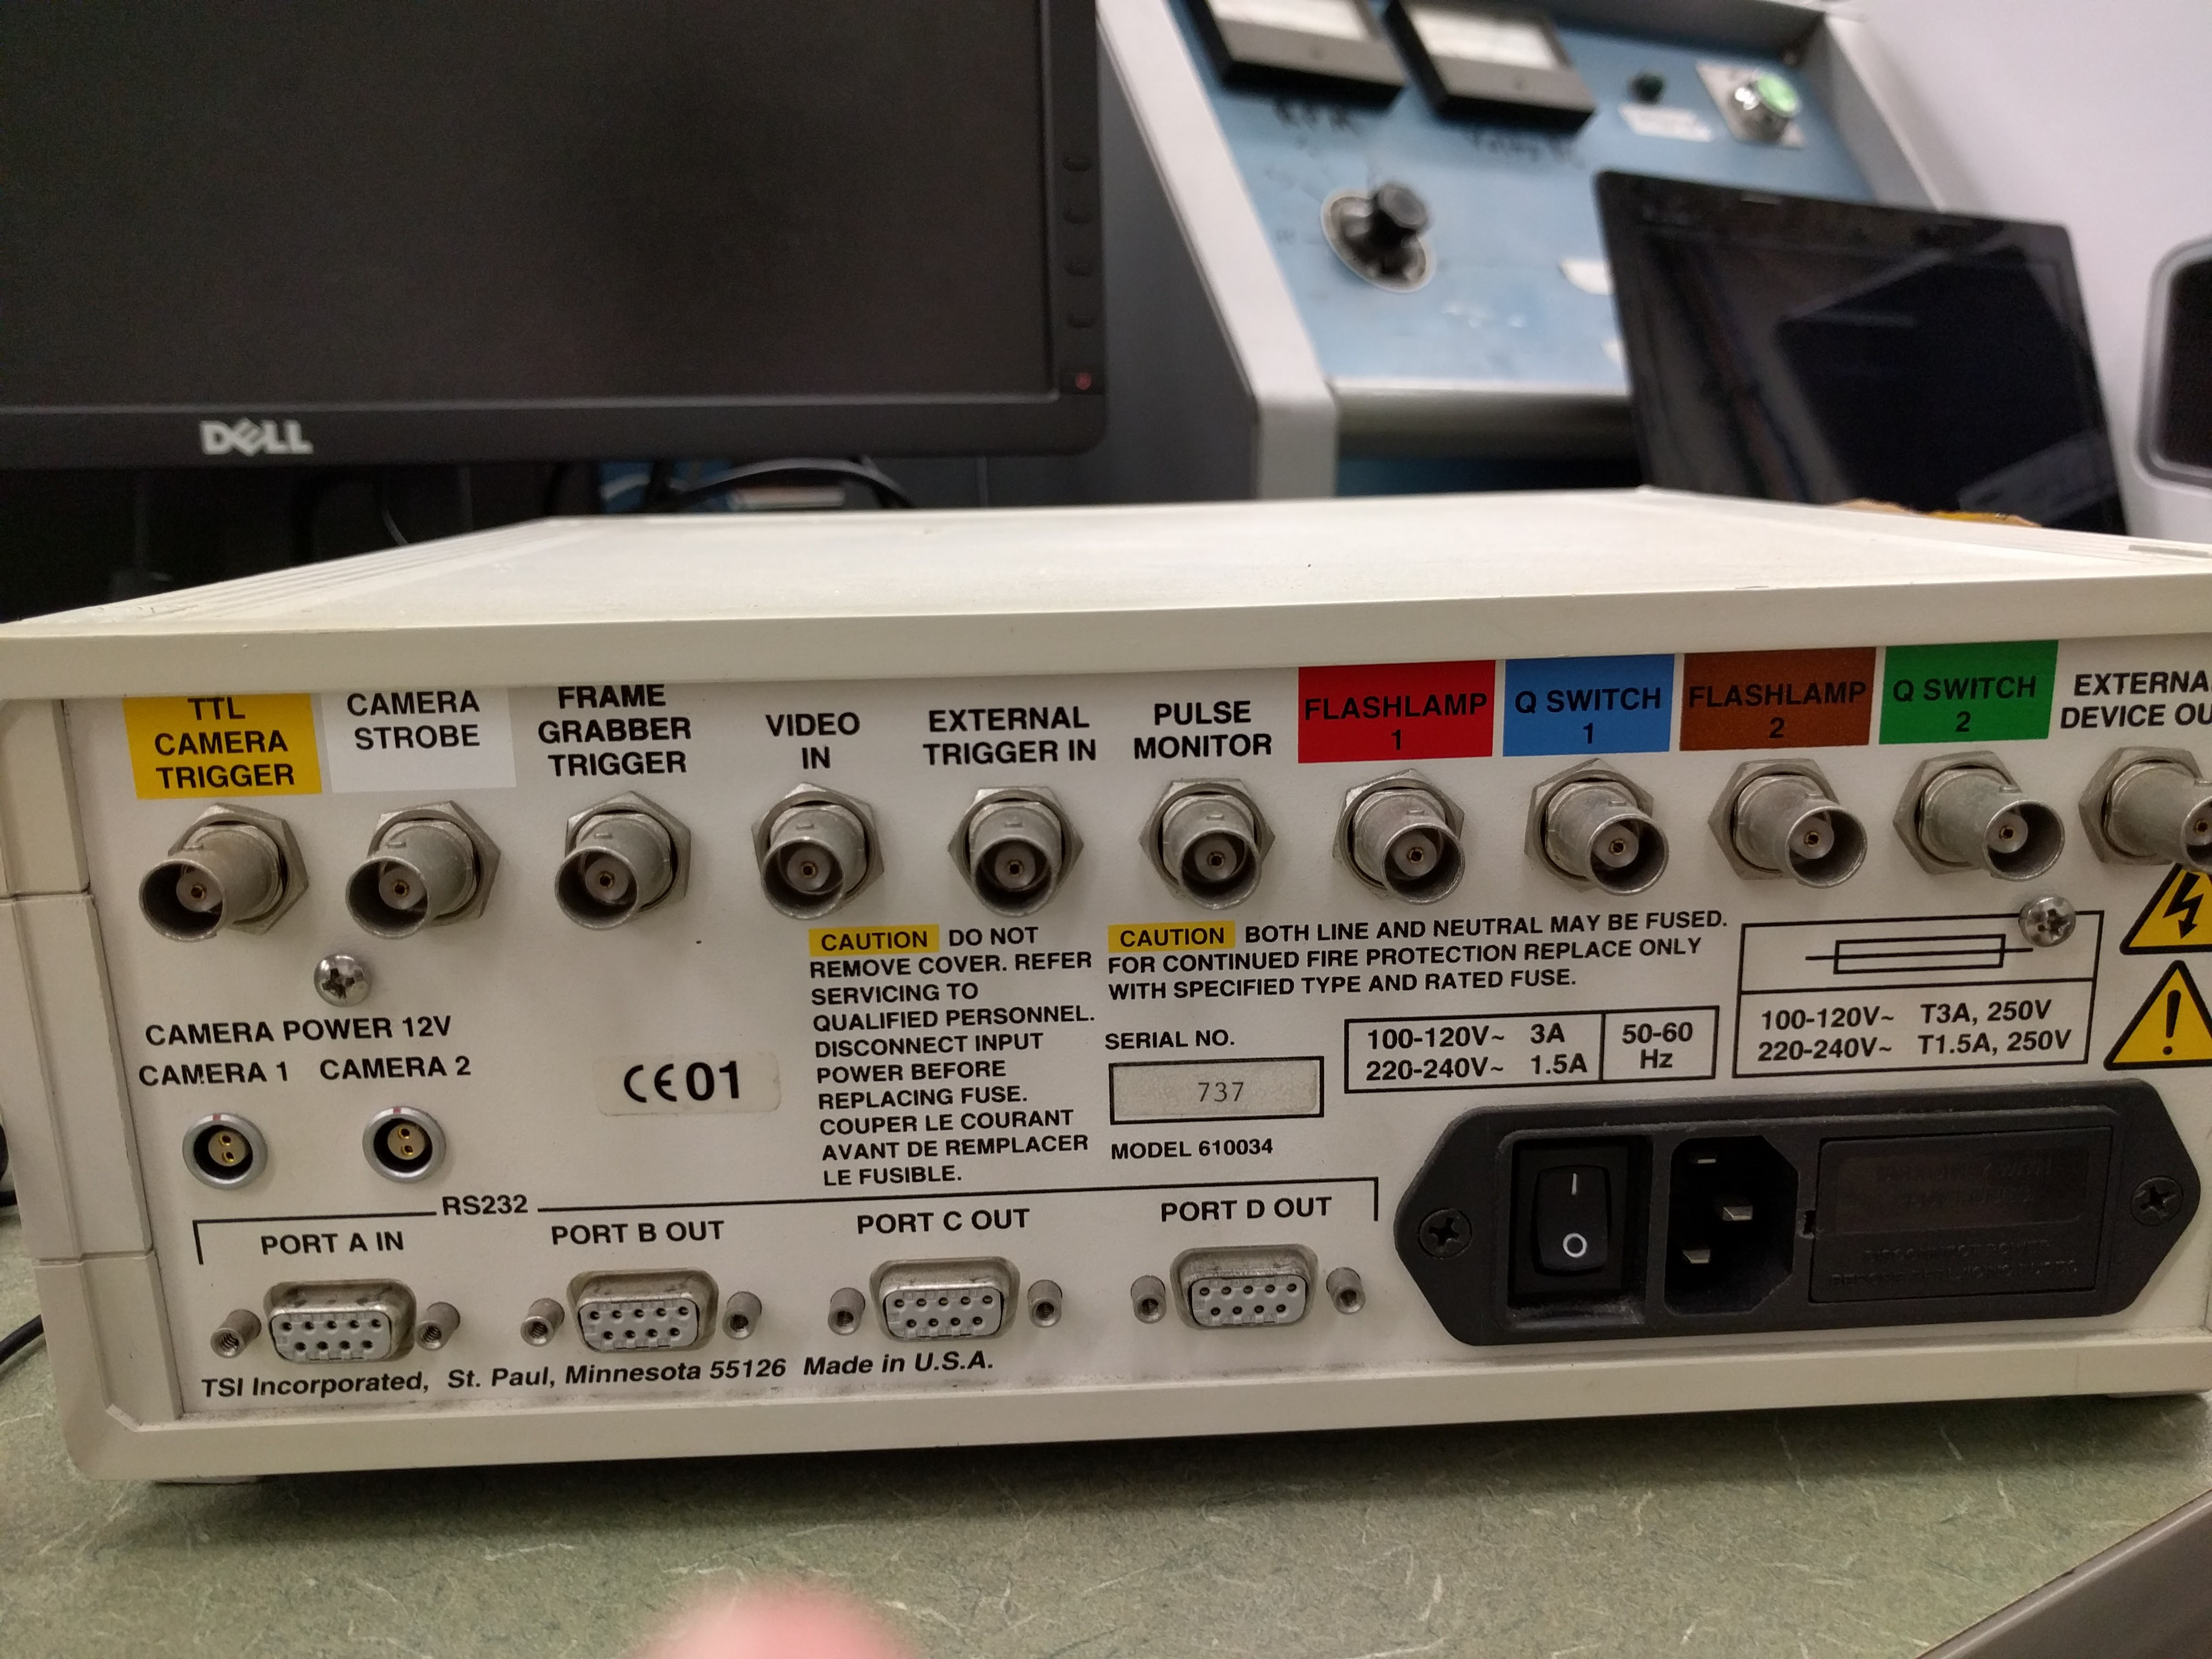
\includegraphics[width=5in]{figs/piv_method/synchronizer_rear}
	\caption{Photograph of synchronizer connectors. Model 610034}
	\label{fig:synchronizer2}
\end{figure}

\begin{figure}[H]
	\centering
	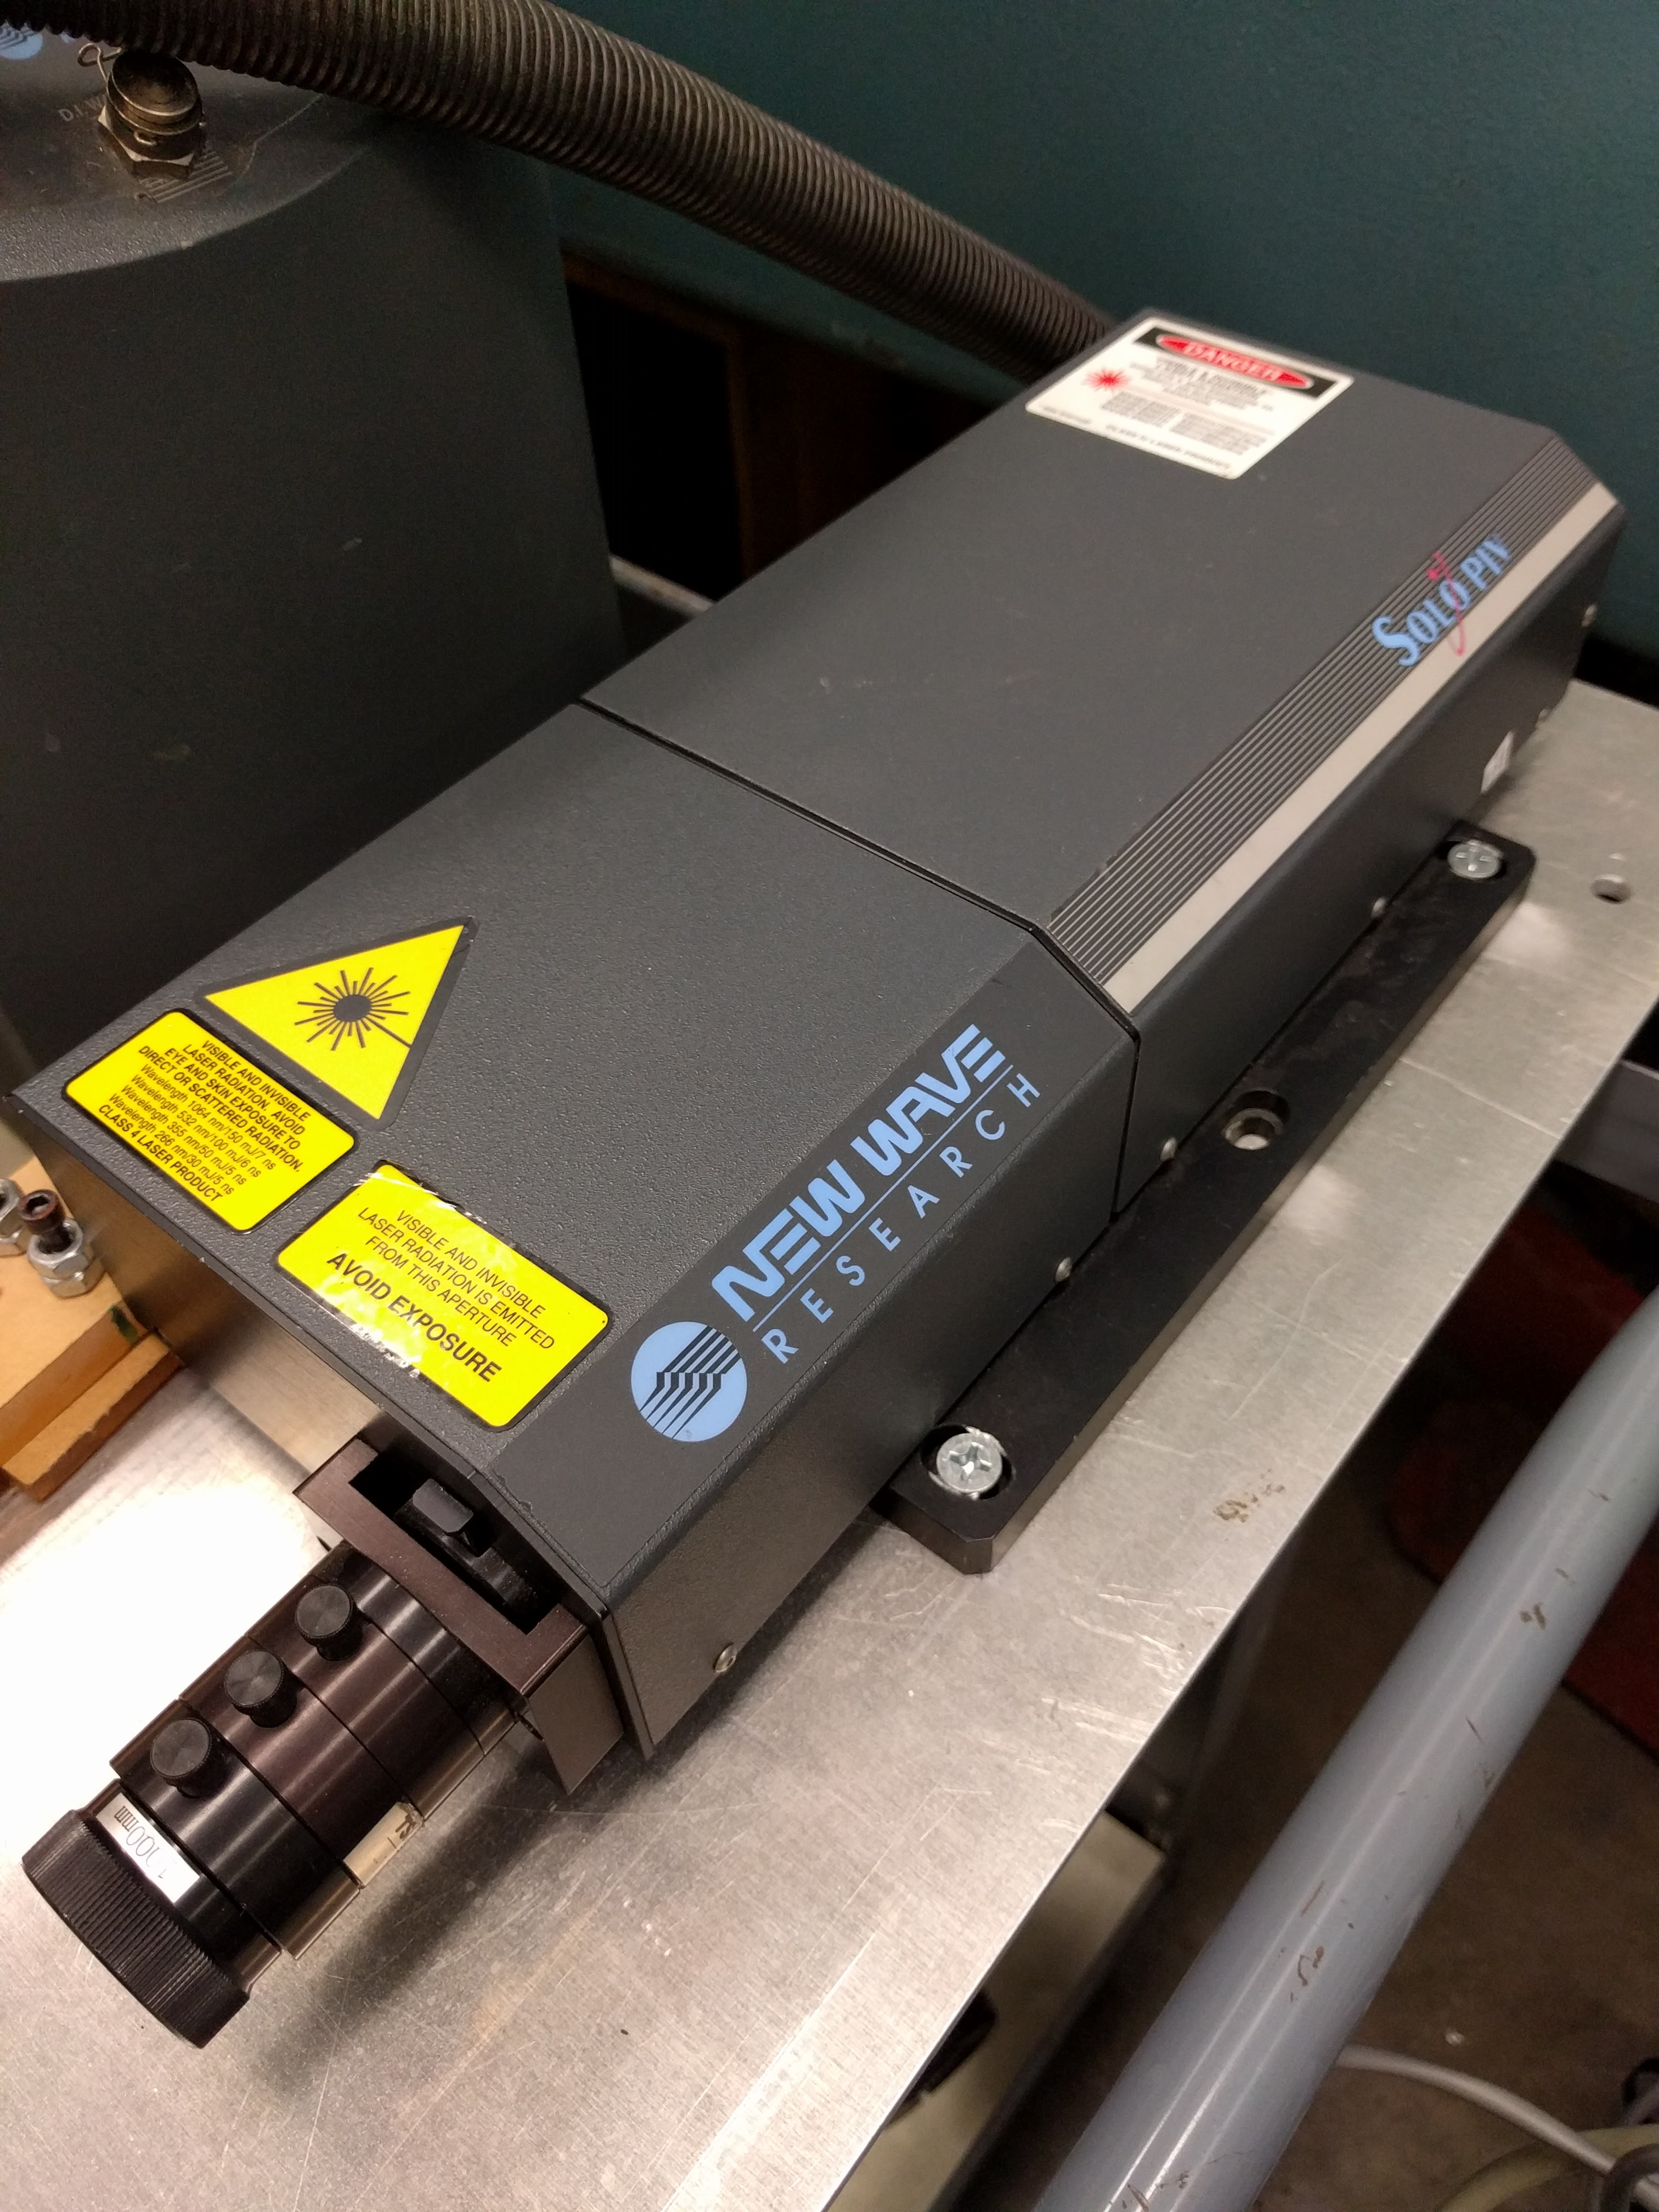
\includegraphics[width=5in]{figs/piv_method/laser}
	\caption{Photograph of a PIV laser by SoloPIV. Model 610034}
	\label{fig:laser}
\end{figure}

\begin{figure}[H]
	\centering
	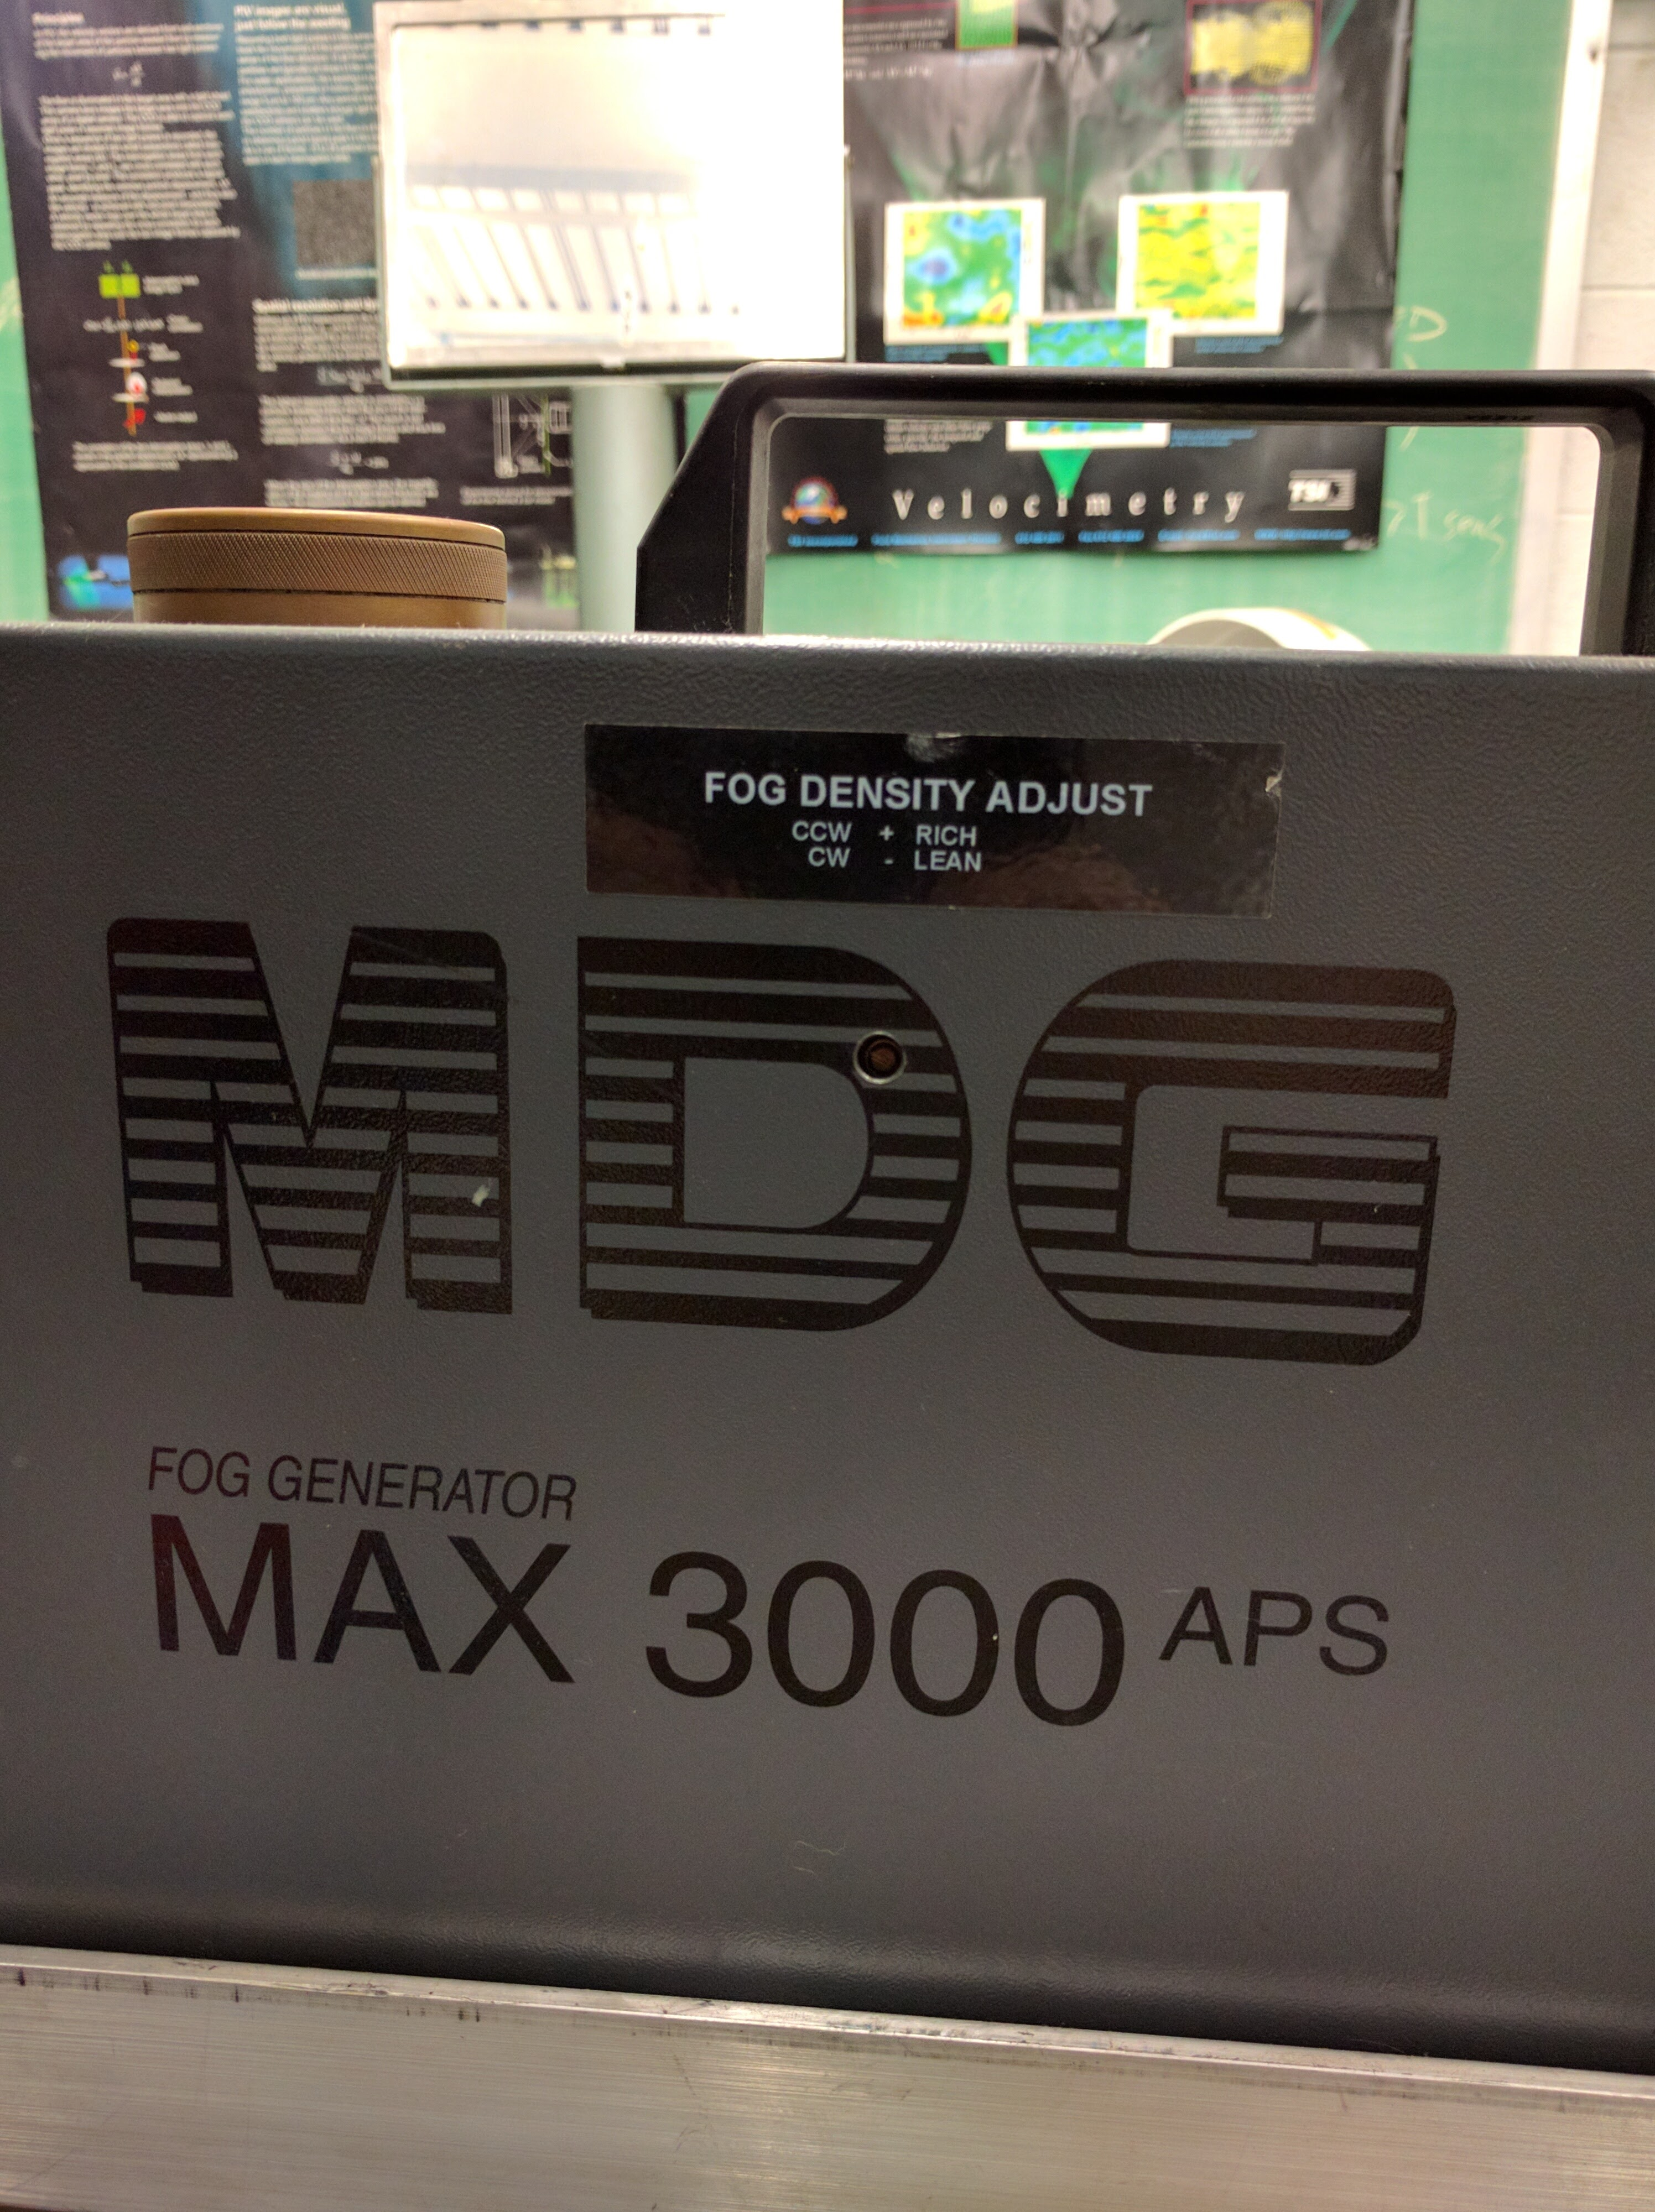
\includegraphics[width=5in]{figs/piv_method/fog_generator}
	\caption{Photograph MDG MAX 3000APS Fog Generator.}
	\label{fig:fog_machine}
\end{figure}

%\begin{figure}[H]
%	\centering
%	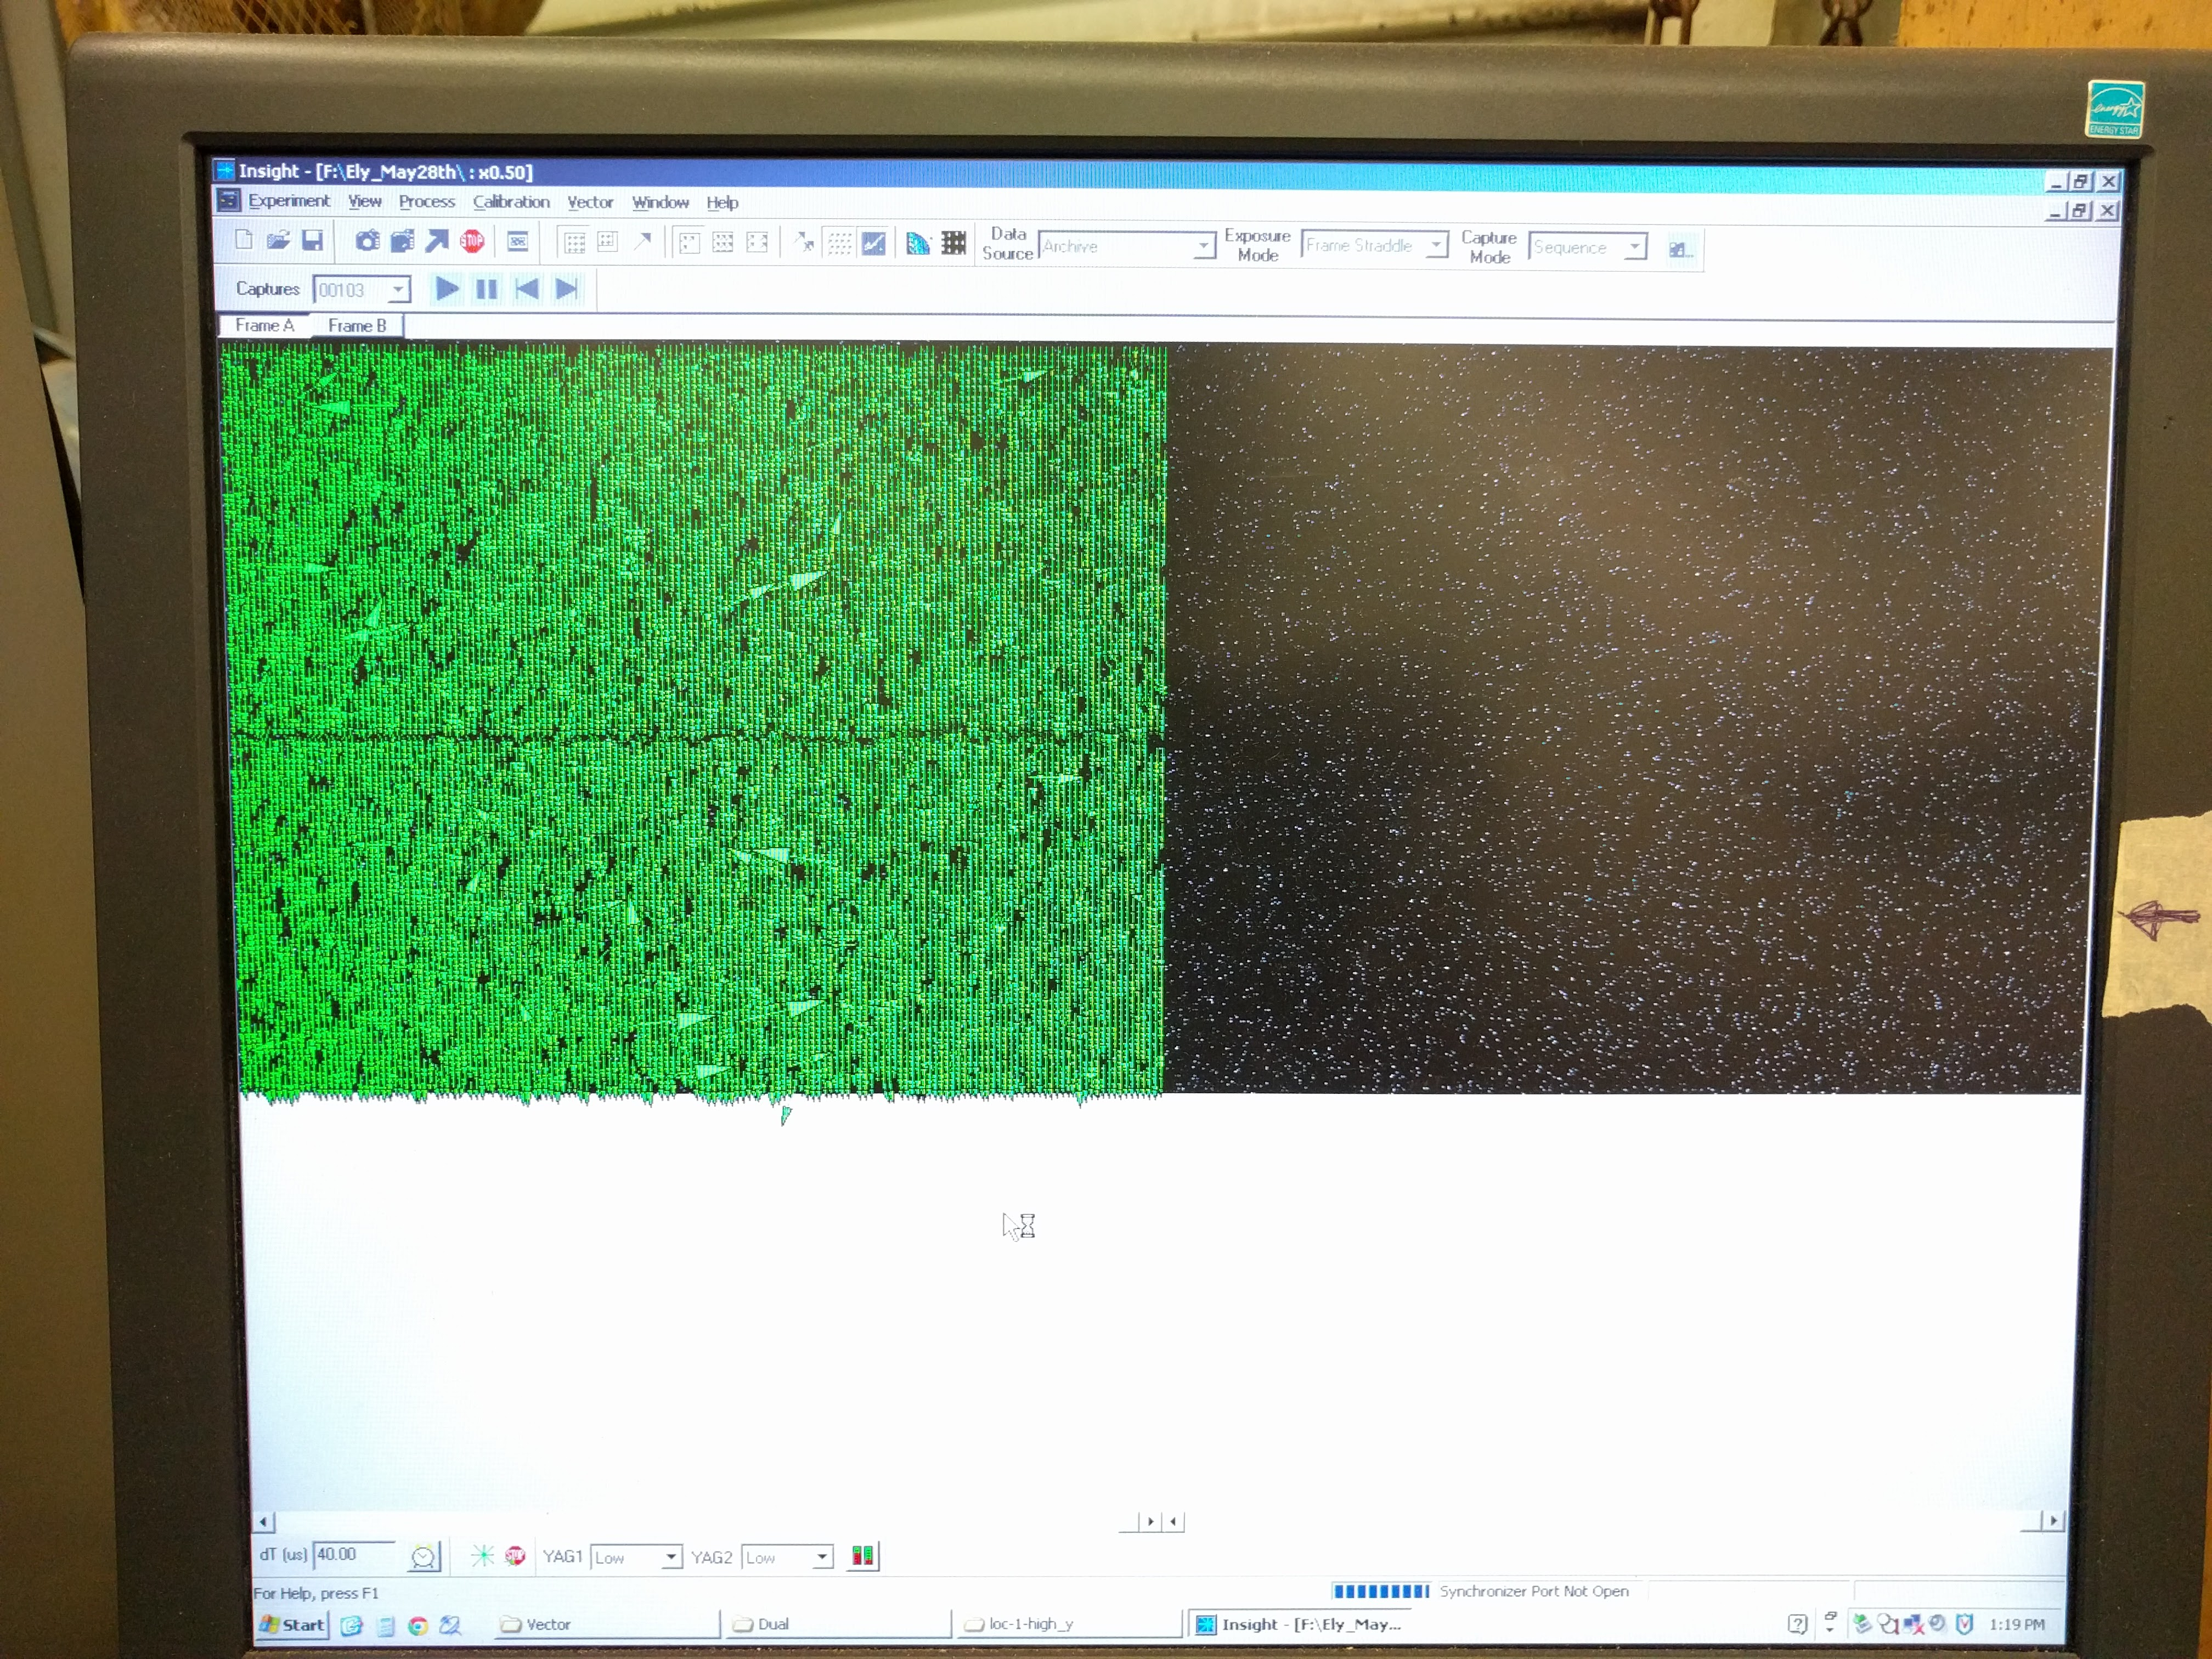
\includegraphics[width=5in]{figs/piv_method/INSIGHT_processing}
%	\caption{Photograph of INSIGHT software computing stereo velocity fields}
%	\label{fig:processing_screenshot}
%\end{figure}

\subsection{Synchronizing the Cameras and Laser}
In order to resolve particle displacements on such a small scale in a 
relatively fast moving fluid, the time interval between a laser pulse sequence 
must be tuned to allow sufficient particle displacement occur to obtain a 
meaningful velocity measurement. If the time interval ($dt$) between successive 
exposures was too long, the particles escaped the interrogation plane, and 
could not be tracked. This study varied the laser pulse timing 
between 25 microseconds for higher wind tunnel speeds, and 50 microseconds for 
slower vortex velocities associated with slower wind tunnel speed. As 
introduced in Chapter 1, this PIV system employed a frame straddling technique, 
which initiates the first shutter opening well before the first laser 
pulse begins such that the camera shutter first closes at as the first laser 
pulse is ending, but before the second laser pulse starts. The second exposure 
begins just as the second laser pulse is initiating, though it extends well 
beyond the termination of the first laser pulse as shown schematically in 
Figure \ref{fig:frame_straddling}. 

\begin{figure}
	\centering
	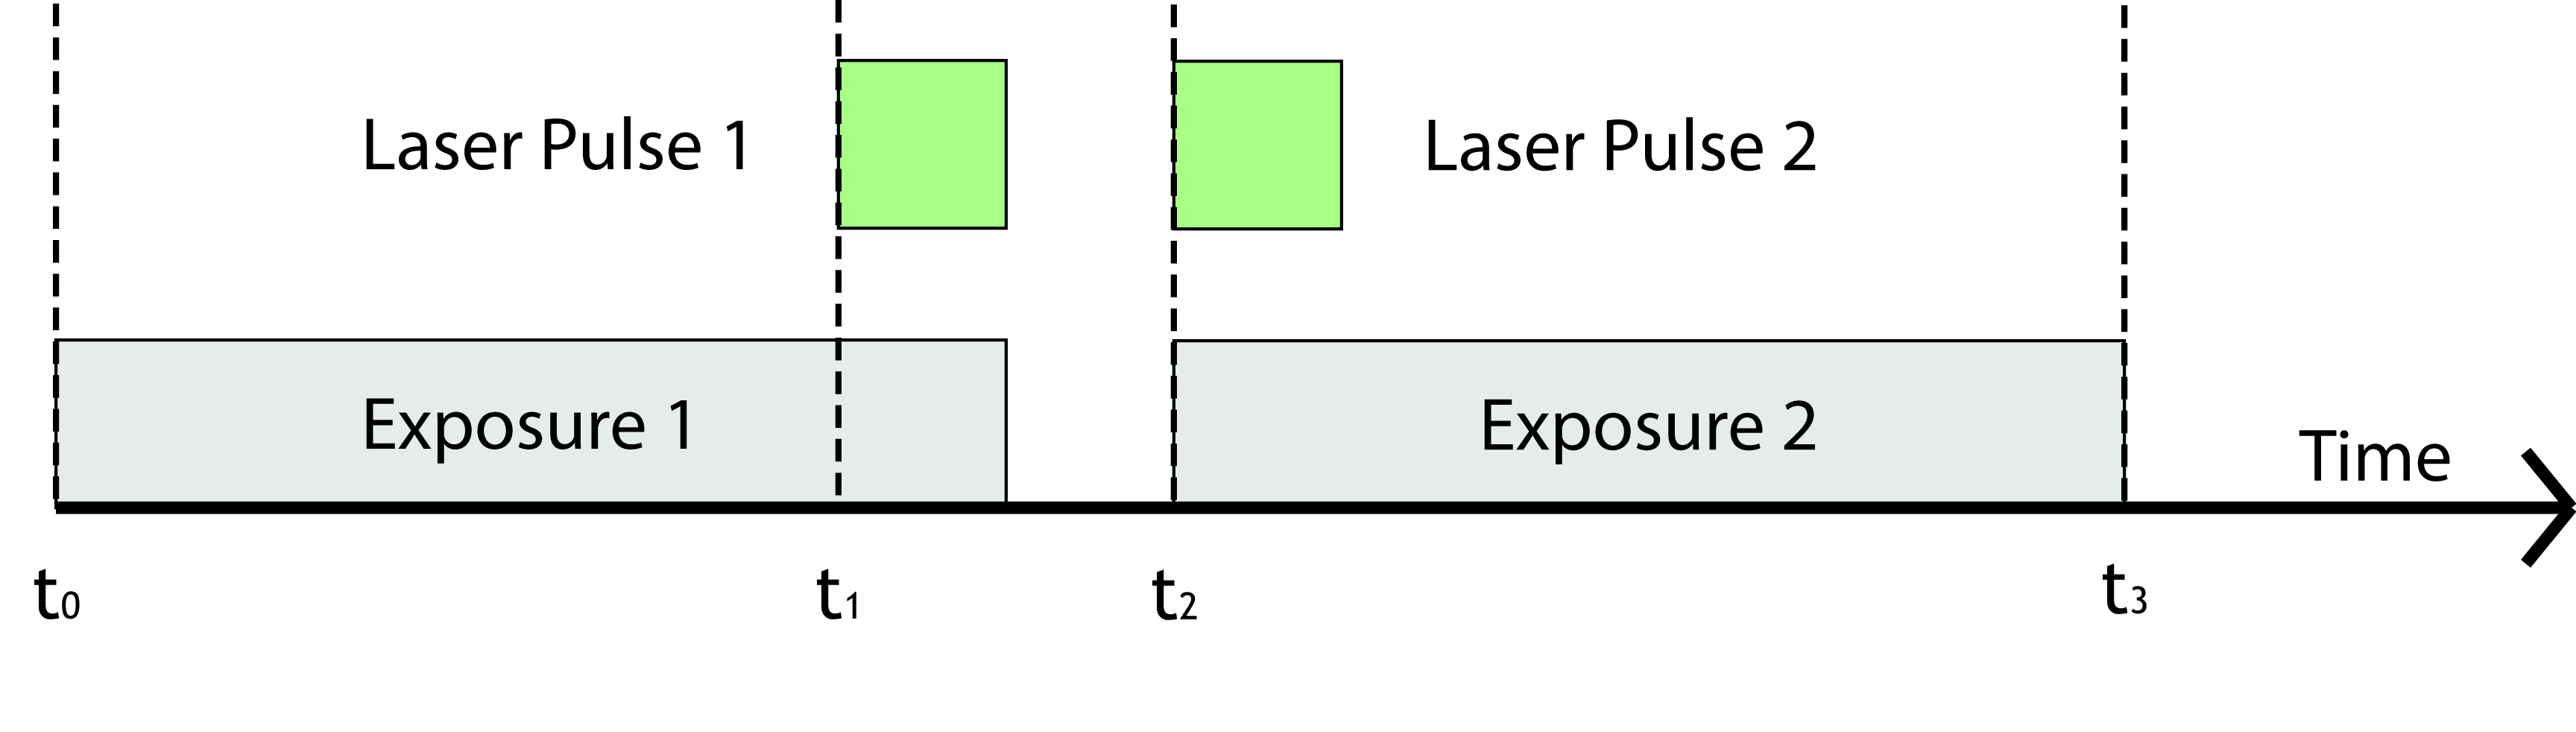
\includegraphics[width=5.5in]{figs/piv_method/frame_straddling}
	\caption{Frame straddling technique. Laser pulses are shown in green, and 
		camera exposures are shown in gray.}
	\label{fig:frame_straddling}
\end{figure}

Timing is achieved with a TSI synchronizer (Figure \ref{fig:synchronizer}) and 
control PC shown in Figure 
\ref{fig:pivblockdiagram}. The control PC sends a command to the synchronizer 
to take an image sample, then the synchronizer sends precisely timed signals to 
operate both cameras and the laser control unit. The cameras each store the 
image pair in an internal memory buffer before returning the data to the 
control PC.

\begin{figure}[H]
	\centering
	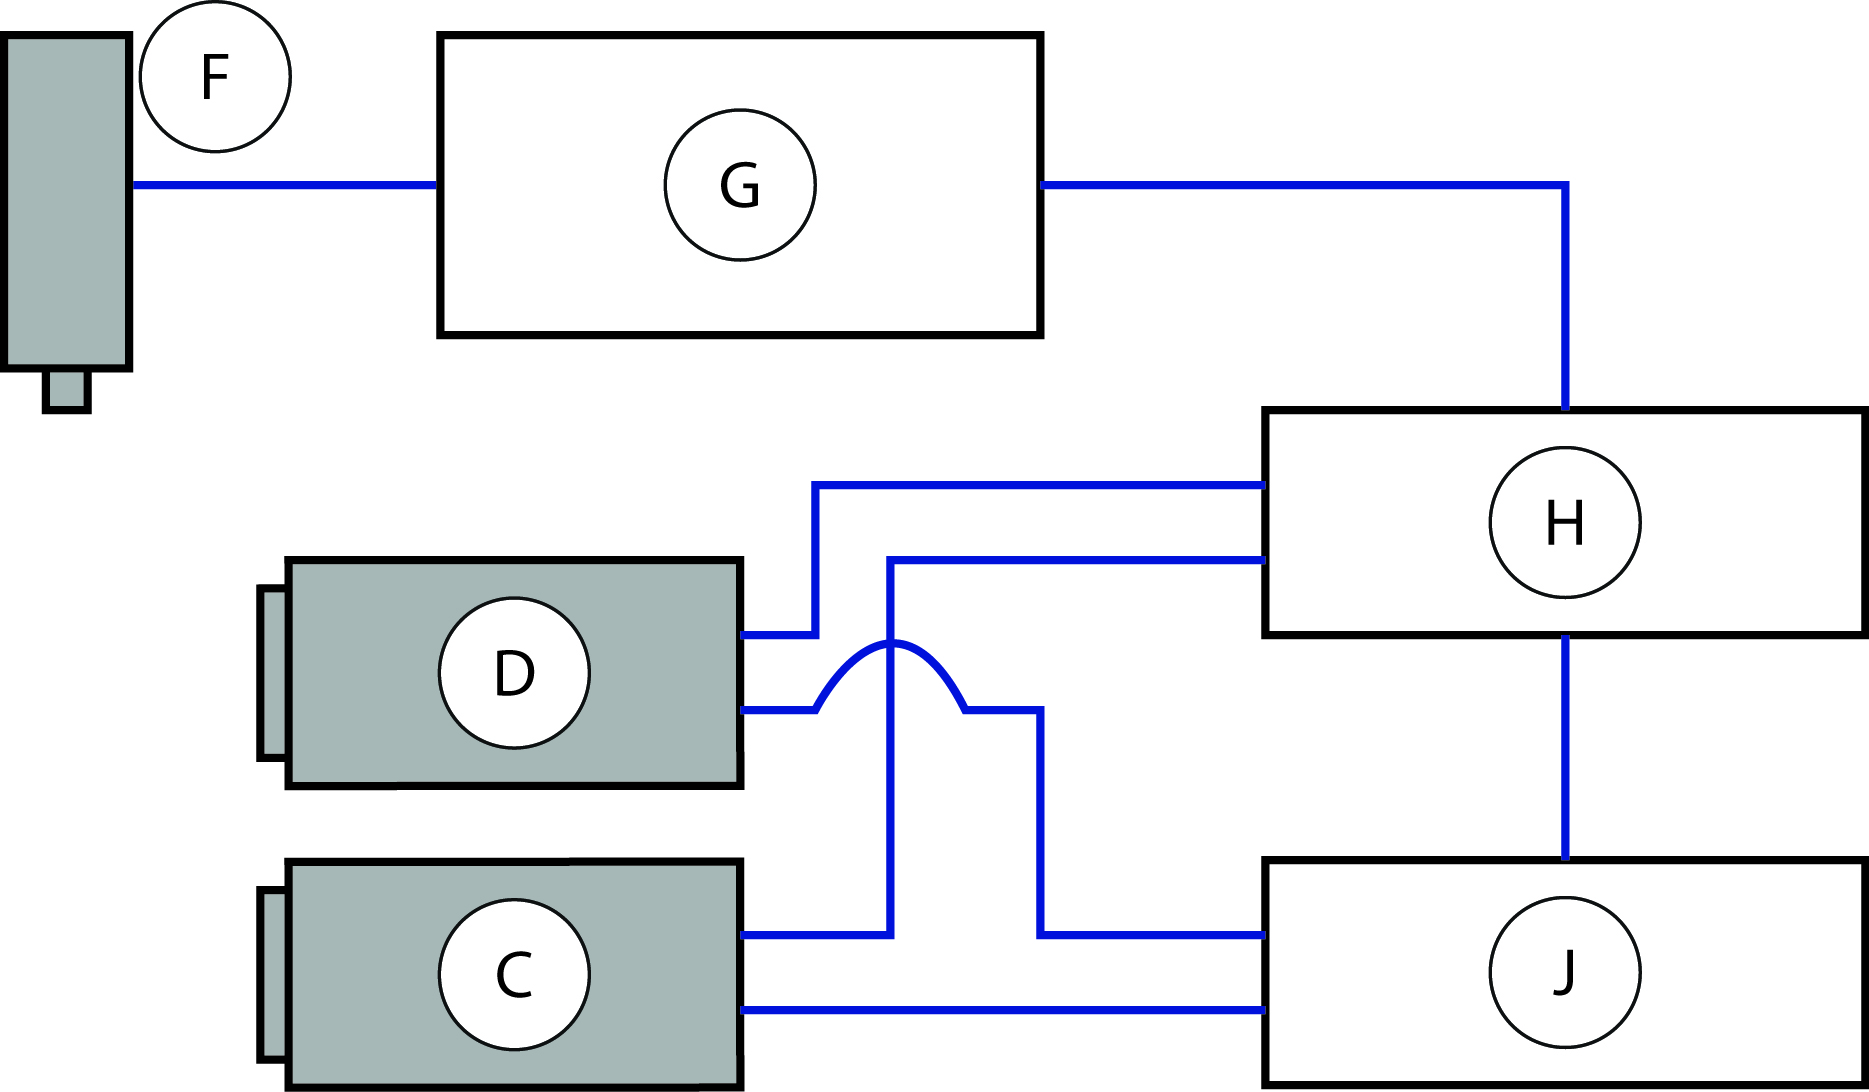
\includegraphics[width=4in]{figs/piv_method/experiment_block_diagram}
	\caption{Block diagram of PIV hardware components. C-left camera, D-right 
		camera, F-Nd:YAG laser, G-laser control unit and power supply, 
		H-synchronizer, 
		J-control PC running INSIGHT software suite.}
	\label{fig:pivblockdiagram}
\end{figure}

\subsection{Calibration employing a PIV Target}

Dimensional calibration was accomplished with the use of a calibration target, 
which was a 10$cm$ by 10$cm$ black calibration plate with precisely positioned 
white divots and a center fiducial mark ,as shown in figure 
\ref{fig:calibration_target}. The calibration target was positioned inside the 
tunnel test section and aligned with the desired interrogation plane. 
The laser illumination sheet was operated in a continuous firing mode and aimed 
into the test section so that the location of the interrogation sheet is 
clearly visible with the use of polarized eye protecting goggles. The camera 
facing surface of the 
interrogation target is then manually aligned with the interrogation plane, 
which was visible as an intense line of light with a nominal thickness of 
1.5$mm$ observable across the top of the target. Once the calibration target 
was properly aligned, the laser and all other light sources in the laboratory 
were extinguished and a lamp was placed downstream of the test section (to 
create ideal lighting conditions) in order to illuminate the target for camera 
focusing. Cameras outfitted with 50mm lenses were manually aimed at the 
calibration target, taking care to place the fiducial mark near the center of 
the image frame. Focusing was accomplished manually by adjusting each lens, and 
a limited PIV data set was created after focusing to ensure that the focus was 
sharp enough to resolve a partially complete velocity vector field within the 
interrogation plane.

\begin{figure}[H]
	\centering
	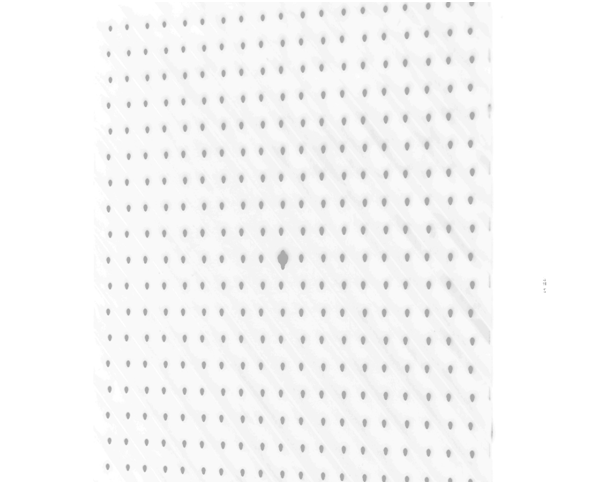
\includegraphics[width=4in]{figs/piv_method/calibration_target}
	\caption{Inverted color and elevated contrast photograph of the calibration 
		target, highlighting the central fiducial mark.}
	\label{fig:calibration_target}
\end{figure}


INSIGHT\textsuperscript{\textcopyright} software was used to take snapshots and 
view them to ensure proper focus 
and alignment. Once satisfactory adjustments were obtained, calibration images 
were taken and the imaging software was used to recognize the fiducial mark, as 
well as each divot, in order to create the necessary two dimensional coordinate 
transformation maps that relate
pixel distance to physical distance. This calibration was employed both to 
determine the magnitudes of the two dimensional velocity vectors unique to each 
camera, and aligning the two separate vector fields, in order to create a three 
dimensional velocity field. Once calibration images were acquired, the 
target was removed and data were taken over a range of velocities in 
that interrogation plane. Each interrogation plane was defined by its position 
downstream relative to the trailing edge of the vortex generator center body. 
Seven interrogation planes were utilized in this study, and every time the 
survey plane was changed, it was necessary to repeat the calibration process. 
Ideally, as dictated by good design of experiments 
practice, the order of experiments should be randomized. This, however, would 
have required exclusive tunnel use for a longer period of time than could be 
scheduled due to the level of demand at the time.

\subsection{Seeding the Flow}

Gathering data with a PIV system requires the flow be properly seeded with 
observable particles. Particles should be sufficiently small to be entrained in 
the flow such that particle motion and fluid motion are the same. In the 
present study, $CO_2$ filled mineral oil bubbles generated with an MDG MAX 3000 
APS fog generator with a Laskin nozzle were used as particle seed. These 
droplets have a nominal diameter of 0.6 micrometers and densities of 1.55 times 
that of air were used \cite{mdgfog}. This was within the optimal range of 
particle densities for good particle entrainment and representation of the 
fluid flow as defined by \cite{mei1996}, as discussed in Chapter 1.

Each velocity measurement 
required a sector of pixels through which displacement could be tracked. If 
a majority of the illuminated particles were allowed to travel outside of a 
given sector between consecutive frame straddled image captures, a meaningful 
correlation map could not be generated. Care was taken to ensure that the 
observable particles 
traversed no more than 50\% of a sector width during the time interval between 
images by adjusting the time interval between image captures ($dt$). 
Utilization of a 50\% border when processing each sector, as described in the 
previous section, helped to ensure that particles did not escape the 
interrogation area. A sufficient quantity of particle groups must be visible in 
each sector in order to yield a meaningful correlation map. If the particle 
seed density was too low, or too high, it would result in a somewhat 
homogeneous image, with ambiguous peaks in the correlation map. A situation 
which results in an increased frequency of spurious measurements with a 
poor signal to noise ratio. Manipulation of sector size 
can increase the number of particles and the reliability of the correlation 
mapping, but only at the expense of reduced velocity field resolution, since 
more pixels are required to resolve each vector.  The amount of mineral oil fog 
(seed) was not controllable in a quantitative manner over an extended period of 
testing, because the dissipation rate was slow enough to disallow complete 
evacuation and re-seeding between experiments, but fast enough to require 
occasional injections of more fog over the course of several hours of 
experimentation. Additional fog was added to the tunnel through a hose inserted 
in the tunnel wall, far upstream of the high speed test section, on a 
qualitative basis. Prior to actual PIV data acquisition, a few test PIV images 
were captured, and a low quality two dimensional computation was performed real 
time for a heads-up evaluation of data quality. On occasion, observed low data 
quality indicated a low particle density in the tunnel, 
so additional particle fog was injected.


\subsection{Pressure Measurements}

Pressure measurements within the vortex core could assist in verifying the 
predicted non-eqiulirbium pressure influences on the behavior of axial wake 
vortices, especially when combined with simultaneous three dimensional 
turbulence measurements with PIV \cite{ash2011}.


Initially, it was believed that a pressure probe could be positioned 
along the axis of the vortex core. Without positioning the probe in many 
locations across the flow and post-processing the data set, it was necessary to 
have some other way to verify that the pressure probe was in fact positioned 
within the vortex core. Simultaneous PIV and pressure measurements were 
attempted utilizing a seven hole probe, but the probe and probe mounting system 
was found to severely obstruct the PIV laser sheet and camera views, cast a 
shadow to obscure flow underneath it, and 
created bright reflections that saturated the image values in the vicinity of 
the vortex. No usable PIV data could be obtained when the a pressure probe was 
mounted in the tunnel test section. Direct visual inspection of the actual 
vortex core employing a continuous laser sheet, revealed that the core appeared 
to dilate significantly in the presence of the pressure probe. Without a method 
to compensate for this potential core dilation, pressure measurements of the 
vortex core region have not been included in this study. It is possible that, 
with a much larger vortex core which is expected to be less 
sensitive to the presence of an inserted pressure probe, and when coated with 
a flat black non-reflective coating utilizing forward mounted PIV cameras 
looking downrange, simultaneous vortex core pressure measurements and PIV 
measurements could be obtained.

\subsection{Capturing PIV Images}

The experiments were conducted with the interrogation plane at seven 
downstream  locations between and 546$mm$ and 1016$mm$. Each of these 
downstream locations will be referred to as a "station" as shown in Figure 
\ref{fig:station_diagram}. Tests were conducted 
starting nearest to the vortex 
generator and progressing downstream. Since changing the position of the 
interrogation plane required a complete re-calibration of the PIV system, the 
order of each test, as defined by its downstream position and velocity, was not 
randomized. For each station, data were taken for each of 
the ten test velocities between 15$m/s$ and 33$m/s$ in ascending order, gaining 
speed over time. Image pairs were acquired once per second, for a period of 200 
seconds, generating a total of 200 image sets. Each test set of images was then 
processed using INSIGHT\textsuperscript{\textcopyright} software in 
order to produce text files containing three-dimensional vector fields for each 
image set in real $(X, Y, Z)$ coordinates.

\begin{figure}[H]
	\centering
	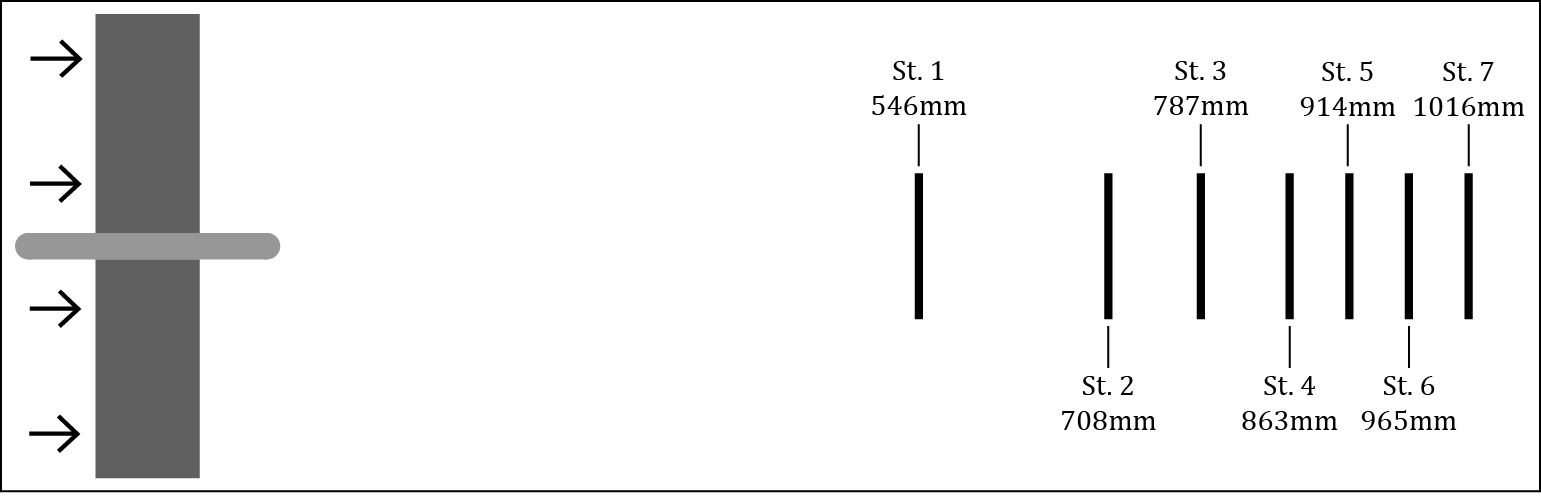
\includegraphics[width=6in]{figs/setup/station_diagram}
	\caption{Diagram showing positions of seven measurement stations taken in 
		two-dimensional planar slices, distances behind vortex generator to 
		scale.}
	\label{fig:station_diagram}
\end{figure}

Tunnel conditions were monitored closely and recorded over the duration of each 
test. In addition, wet bulb and dry bulb temperatures were taken with a sling 
psychrometer. Specific details for each test including the relative humidity 
($\phi$) estimated from wet bulb and dry bulb temperature measurements and the
associated pressure relaxation coefficient 
($\eta_P$), are summarized in Tables \ref{table:station_1_measurements} through 
\ref{table:station_7_measurements}. 

Nominal velocity is denoted $V_{nom}$, while actual mean free stream 
velocity is denoted $V_{fs}$, and variance in the measurement for the 
duration of the test is labeled $\sigma_{V_{fs}}$. Dynamic pressure is $Q$, 
atmospheric 
pressure is $P_{atm}$, and the tunnel temperature is $T_{tunnel}$. Free stream 
velocity was calculated from dynamic pressure via

\begin{equation}
q = \frac{1}{2}\rho V^2
\end{equation}
\noindent
and
\begin{equation}
P = \rho R T
\end{equation}

Relative 
humidity $\phi$ was calculated from wet bulb and dry bulb temperatures ($T_w$ 
and $T$, respectively) by 
equations \ref{eq:rh_es} through \ref{eq:rh_rh} according to \cite{owen1977}. 
Finally, pressure relaxation coefficient is calculated according to the table 
in \cite{ash2011}.

\begin{equation}
e_S = 6.112 exp \left( \frac{17.67 T}{T + 243.5} \right)
\label{eq:rh_es}
\end{equation}

\begin{equation}
e_W = 6.112 exp \left( \frac{17.67 T_W}{T_W + 243.5} \right)
\label{eq:rh_ew}
\end{equation}

\begin{equation}
e = e_W - P_{atm} (T - T_W) 0.00066(1 +( 0.00115T_W))
\label{eq:rh_e}
\end{equation}

\begin{equation}
\phi = 100 \frac{e}{e_S}
\label{eq:rh_rh}
\end{equation}



\renewcommand\baselinestretch{1.3}\selectfont
\begin{table}[H]
\begin{center}
\begin{tabular}{|ccccccccccc|}
	\hline
	Run & $I_Z$ & $V_{nom}$ & $dt$ & $V_{fs}$ & $\sigma_{V_{fs}}$ & $Q$ & $P_{atm}$ & $T_{tunnel}$ & $\phi$ & $\eta_P$\\
	$ID$ & $(mm)$ & $(m/s)$ & $(\mu s)$ & $(m/s)$ & $(m/s)$ & $(Pa)$ & $(Pa)$ & $(\degree K)$ & $(\%)$ & $(\mu s)$\\
	\hline
	1 & 546 & 15 & 50 & 15.22 & 0.02 & 135 & 102036 & 299.85 & 60.4 & 0.35\\
	2 & 546 & 17 & 50 & 16.88 & 0.02 & 170 & 102115 & 297.55 & 66.3 & 0.329\\
	3 & 546 & 19 & 50 & 19.43 & 0.01 & 225 & 102105 & 297.55 & 66.3 & 0.329\\
	4 & 546 & 21 & 50 & 21.06 & 0.02 & 264 & 102100 & 297.75 & 66.3 & 0.324\\
	5 & 546 & 23 & 35 & 23.21 & 0.04 & 321 & 102097 & 297.95 & 66.3 & 0.324\\
	6 & 546 & 25 & 35 & 24.86 & 0.05 & 371 & 102093 & 298.15 & 66.3 & 0.324\\
	7 & 546 & 27 & 35 & 27.02 & 0.03 & 434 & 102092 & 298.3 & 66.3 & 0.324\\
	8 & 546 & 29 & 25 & 29.12 & 0.04 & 505 & 102080 & 298.35 & 66.3 & 0.324\\
	9 & 546 & 31 & 25 & 30.86 & 0.06 & 564 & 102050 & 299.15 & 66.3 & 0.324\\
	10 & 546 & 33 & 25 & 32.98 & 0.05 & 641 & 102054 & 299.9 & 60.4 & 0.35\\
	\hline
\end{tabular}
\caption{Experimental measurements for station 1}
\label{table:station_1_measurements}
\end{center}
\end{table}
\renewcommand\baselinestretch{2}\selectfont

\renewcommand\baselinestretch{1.3}\selectfont
\begin{table}[H]
\begin{center}
\begin{tabular}{|ccccccccccc|}
	\hline
	Run & $I_Z$ & $V_{nom}$ & $dt$ & $V_{fs}$ & $\sigma_{V_{fs}}$ & $Q$ & $P_{atm}$ & $T_{tunnel}$ & $\phi$ & $\eta_P$\\
	$ID$ & $(in)$ & $(m/s)$ & $(\mu s)$ & $(m/s)$ & $(m/s)$ & $(Pa)$ & $(Pa)$ & $(\degree K)$ & $(\%)$ & $(\mu s)$\\
	\hline
	11 & 708 & 15 & 40 & 15.27 & 0.02 & 138 & 101185 & 296.05 & 69.8 & 0.312\\
	12 & 708 & 17 & 40 & 16.89 & 0.02 & 169 & 101218 & 296.55 & 69.8 & 0.312\\
	13 & 708 & 19 & 40 & 19.03 & 0.02 & 215 & 101219 & 296.55 & 69.8 & 0.312\\
	14 & 708 & 21 & 40 & 21.13 & 0.02 & 264 & 101186 & 296.85 & 66.3 & 0.329\\
	15 & 708 & 23 & 40 & 23.21 & 0.04 & 321 & 101150 & 297.85 & 66.8 & 0.329\\
	16 & 708 & 25 & 25 & 25.36 & 0.04 & 380 & 101120 & 297.45 & 71.7 & 0.301\\
	17 & 708 & 27 & 25 & 27.03 & 0.03 & 432 & 101120 & 297.75 & 70.1 & 0.306\\
	18 & 708 & 29 & 25 & 29.12 & 0.06 & 498 & 101106 & 298.55 & 73.3 & 0.297\\
	19 & 708 & 31 & 25 & 30.87 & 0.04 & 562 & 101109 & 298.95 & 73.3 & 0.297\\
	20 & 708 & 33 & 25 & 33.39 & 0.04 & 653 & 101101 & 299.65 & 73.3 & 0.297\\
	\hline
\end{tabular}
\caption{Experimental measurements for station 2}
\label{table:station_2_measurements}
\end{center}
\end{table}
\renewcommand\baselinestretch{2}\selectfont

\begin{table}[H]
\begin{center}
\begin{tabular}{|ccccccccccc|}
	\hline
	Run & $I_Z$ & $V_{nom}$ & $dt$ & $V_{fs}$ & $\sigma_{V_{fs}}$ & $Q$ & $P_{atm}$ & $T_{tunnel}$ & $\phi$ & $\eta_P$\\
	$ID$ & $(in)$ & $(m/s)$ & $(\mu s)$ & $(m/s)$ & $(m/s)$ & $(Pa)$ & $(Pa)$ & $(\degree K)$ & $(\%)$ & $(\mu s)$\\
	\hline
	21 & 787 & 15 & 40 & 15.2 & 0.02 & 136 & 101094 & 297.95 & 72 & 0.295\\
	22 & 787 & 17 & 40 & 17.27 & 0.02 & 176 & 101100 & 297.85 & 72 & 0.295\\
	23 & 787 & 19 & 40 & 19.36 & 0.03 & 222 & 101102 & 297.95 & 70.2 & 0.305\\
	24 & 787 & 21 & 40 & 21.09 & 0.03 & 262 & 101088 & 297.95 & 75.3 & 0.287\\
	25 & 787 & 23 & 40 & 23.15 & 0.02 & 316 & 101079 & 298.05 & 75.3 & 0.287\\
	26 & 787 & 25 & 25 & 24.86 & 0.02 & 364 & 101062 & 298.45 & 71.9 & 0.298\\
	27 & 787 & 27 & 25 & 26.95 & 0.04 & 430 & 101054 & 298.65 & 70.2 & 0.305\\
	28 & 787 & 29 & 25 & 29.09 & 0.04 & 496 & 101051 & 299.05 & 71.9 & 0.298\\
	29 & 787 & 31 & 25 & 31.26 & 0.04 & 576 & 101056 & 299.35 & 71.9 & 0.298\\
	30 & 787 & 33 & 25 & 32.94 & 0.04 & 636 & 101024 & 299.75 & 77 & 0.283\\
	\hline
\end{tabular}
\caption{Experimental measurements for station 3}
\label{table:station_3_measurements}
\end{center}
\end{table}

\begin{table}[H]
\begin{center}
\begin{tabular}{|ccccccccccc|}
	\hline
	Run & $I_Z$ & $V_{nom}$ & $dt$ & $V_{fs}$ & $\sigma_{V_{fs}}$ & $Q$ & $P_{atm}$ & $T_{tunnel}$ & $\phi$ & $\eta_P$\\
	$ID$ & $(in)$ & $(m/s)$ & $(\mu s)$ & $(m/s)$ & $(m/s)$ & $(Pa)$ & $(Pa)$ & $(\degree K)$ & $(\%)$ & $(\mu s)$\\
	\hline
	31 & 863 & 15 & 40 & 14.86 & 0.02 & 133 & 101865 & 295.75 & 63.8 & 0.354\\
	32 & 863 & 17 & 40 & 17.39 & 0.02 & 180 & 101855 & 295.95 & 63.8 & 0.354\\
	33 & 863 & 19 & 40 & 19.08 & 0.02 & 219 & 101847 & 296.1 & 63.8 & 0.354\\
	34 & 863 & 21 & 40 & 21.13 & 0.05 & 267 & 101845 & 296.15 & 63.8 & 0.354\\
	35 & 863 & 23 & 40 & 23.29 & 0.02 & 323 & 101844 & 296.45 & 63.8 & 0.354\\
	36 & 863 & 25 & 25 & 24.98 & 0.05 & 373 & 101840 & 296.65 & 65.6 & 0.344\\
	37 & 863 & 27 & 25 & 27.09 & 0.05 & 438 & 101843 & 297 & 65.6 & 0.344\\
	38 & 863 & 29 & 25 & 28.81 & 0.03 & 493 & 101848 & 297.55 & 65.6 & 0.344\\
	39 & 863 & 31 & 25 & 30.87 & 0.04 & 570 & 101842 & 298.15 & - & -\\
	40 & 863 & 33 & 25 & 33.44 & 0.06 & 661 & 101844 & 298.35 & - & -\\
	\hline
\end{tabular}
\caption{Experimental measurements for station 4}
\label{table:station_4_measurements}
\end{center}
\end{table}

\renewcommand\baselinestretch{1.3}\selectfont
\begin{table}[H]
\begin{center}
\begin{tabular}{|ccccccccccc|}
	\hline
	Run & $I_Z$ & $V_{nom}$ & $dt$ & $V_{fs}$ & $\sigma_{V_{fs}}$ & $Q$ & $P_{atm}$ & $T_{tunnel}$ & $\phi$ & $\eta_P$\\
	$ID$ & $(in)$ & $(m/s)$ & $(\mu s)$ & $(m/s)$ & $(m/s)$ & $(Pa)$ & $(Pa)$ & $(\degree K)$ & $(\%)$ & $(\mu s)$\\
	\hline
	41 & 914 & 15 & 40 & 14.88 & 0.02 & 132 & 101815 & 296.25 & 57.5 & 0.386\\
	42 & 914 & 17 & 40 & 17.24 & 0.03 & 180 & 101812 & 296.35 & 55.8 & 0.398\\
	43 & 914 & 19 & 40 & 19.08 & 0.03 & 217 & 101812 & 294.45 & 55.8 & 0.398\\
	44 & 914 & 21 & 40 & 21.18 & 0.03 & 267 & 101816 & 296.65 & 55.8 & 0.398\\
	45 & 914 & 23 & 40 & 23.24 & 0.03 & 323 & 101809 & 296.95 & 55.8 & 0.398\\
	46 & 914 & 25 & 25 & 24.9 & 0.03 & 371 & 101802 & 297.15 & 55.8 & 0.398\\
	47 & 914 & 27 & 25 & 27.08 & 0.04 & 435 & 101788 & 297.45 & 55.8 & 0.398\\
	48 & 914 & 29 & 25 & 29.19 & 0.03 & 506 & 101784 & 297.85 & 55.8 & 0.398\\
	49 & 914 & 31 & 25 & 31.28 & 0.05 & 584 & 101786 & 298.15 & 56.1 & 0.393\\
	50 & 914 & 33 & 25 & 33.05 & 0.05 & 645 & 101789 & 298.75 & 56.1 & 0.393\\
	\hline
\end{tabular}
\caption{Experimental measurements for station 5}
\label{table:station_5_measurements}
\end{center}
\end{table}
\renewcommand\baselinestretch{2}\selectfont

\begin{table}[H]
\begin{center}
\begin{tabular}{|ccccccccccc|}
	\hline
	Run & $I_Z$ & $V_{nom}$ & $dt$ & $V_{fs}$ & $\sigma_{V_{fs}}$ & $Q$ & $P_{atm}$ & $T_{tunnel}$ & $\phi$ & $\eta_P$\\
	$ID$ & $(in)$ & $(m/s)$ & $(\mu s)$ & $(m/s)$ & $(m/s)$ & $(Pa)$ & $(Pa)$ & $(\degree K)$ & $(\%)$ & $(\mu s)$\\
	\hline
	51 & 965 & 15 & 40 & 15.31 & 0.02 & 140 & 102039 & 294.85 & 61.2 & 0.381\\
	52 & 965 & 17 & 40 & 17.36 & 0.03 & 182 & 102034 & 294.95 & 61.2 & 0.381\\
	53 & 965 & 19 & 40 & 19.08 & 0.03 & 219 & 102035 & 295.15 & 59.5 & 0.392\\
	54 & 965 & 21 & 40 & 21.23 & 0.03 & 270 & 102037 & 295.35 & 59.5 & 0.392\\
	55 & 965 & 23 & 40 & 23.33 & 0.03 & 327 & 102018 & 295.65 & 59.5 & 0.392\\
	56 & 965 & 25 & 25 & 24.97 & 0.03 & 375 & 102021 & 295.95 & 59.5 & 0.392\\
	57 & 965 & 27 & 25 & 27.05 & 0.06 & 437 & 102008 & 297.85 & 52.6 & 0.422\\
	58 & 965 & 29 & 25 & 29.17 & 0.04 & 505 & 102005 & 298.15 & 47.4 & 0.454\\
	59 & 965 & 31 & 25 & 30.9 & 0.06 & 571 & 102015 & 297.85 & 53.7 & 0.421\\
	60 & 965 & 33 & 25 & 33.04 & 0.06 & 653 & 102009 & 297.35 & 53.7 & 0.421\\
	\hline
\end{tabular}
\caption{Experimental conditions for tests at station 6}
\label{table:station_6_measurements}
\end{center}
\end{table}

\begin{table}[H]
\begin{center}
\begin{tabular}{|ccccccccccc|}
	\hline
	Run & $I_Z$ & $V_{nom}$ & $dt$ & $V_{fs}$ & $\sigma_{V_{fs}}$ & $Q$ & $P_{atm}$ & $T_{tunnel}$ & $\phi$ & $\eta_P$\\
	$ID$ & $(in)$ & $(m/s)$ & $(\mu s)$ & $(m/s)$ & $(m/s)$ & $(Pa)$ & $(Pa)$ & $(\degree K)$ & $(\%)$ & $(\mu s)$\\
	\hline
	61 & 1016 & 15 & 40 & 15.31 & 0.03 & 140 & 101977 & 296.15 & 52 & 0.434\\
	62 & 1016 & 17 & 40 & 16.98 & 0.04 & 171 & 101969 & 296.25 & 52 & 0.434\\
	63 & 1016 & 19 & 40 & 19.1 & 0.03 & 218 & 101961 & 296.3 & 52 & 0.434\\
	64 & 1016 & 21 & 40 & 21.15 & 0.05 & 269 & 101950 & 296.45 & 49.4 & 0.45\\
	65 & 1016 & 23 & 25 & 23.23 & 0.05 & 321 & 101953 & 296.77 & 52.6 & 0.422\\
	66 & 1016 & 25 & 25 & 24.96 & 0.05 & 371 & 101951 & 297.07 & 52.6 & 0.422\\
	67 & 1016 & 27 & 25 & 27.05 & 0.5 & 436 & 101936 & 297.25 & 52.6 & 0.422\\
	68 & 1016 & 29 & 25 & 29.17 & 0.03 & 505 & 101928 & 297.76 & 52.6 & 0.422\\
	69 & 1016 & 31 & 25 & 31.31 & 0.05 & 581 & 101921 & 297.85 & 52.6 & 0.422\\
	70 & 1016 & 33 & 25 & 33.01 & 0.05 & 647 & 101922 & 298.3 & 52.6 & 0.422\\
	\hline
\end{tabular}
\caption{Experimental conditions for tests at station 7}
\label{table:station_7_measurements.}
\end{center}
\end{table}


\section{Stereo PIV Data processing}

Raw PIV data was processed into text files containing lists of vectors and 
positions from raw image data with commercial INSIGHT software. 
This format is considered to be the 
starting point for the present analysis. Each vector is recorded as a row in a 
"v3d" file, with a set of position coordinates,velocity 
vector components, and two quality control flags that were used to reduce 
spurious vector count. An example of this data is shown in Table 
\ref{table:v3d_row_example}.

\begin{table}[H]
\begin{center}
\begin{tabular}{|cccccccc|}
	\hline
	X mm & Y mm  & Z mm & U m/s & V m/s & W m/s & CHC & Residual Pixels\\
	\hline
	8.02046 & 0.174553 & 0 & 0.415872 & -2.25951 & 13.5873 & 1 & 0.127058\\
	9.74656 & 0.174553 & 0 & 0.386507 & -2.4523 & 13.9244 & 1 & 0.166965\\
	11.4727 & 0.174553 & 0 & 1.01919 & -2.8773 & 14.9454 & 1 & 0.0480147\\
	13.1988 & 0.174553 & 0 & 1.30872 & -3.02836 & 15.2081 & 1 & 0.0560525\\
	\hline
\end{tabular}
\caption{Example rows from v3d files with raw 3d vector data}
\label{table:v3d_row_example}
\end{center}
\end{table}


The position coordinates are expressed in units of millimeters from 
the fiducial mark on the target used for calibration. These coordinates are 
expressed from the viewpoint of the cameras, which were pointed upstream; 
positive $X$ coordinates are to the right, positive $Y$ is upwards, and 
positive $Z$ is towards the cameras. Vector components are recorded as $U$, 
$V$ and $W$. 

\subsection{Notation}
Since each run contained 200 separate vector sets, this data must be 
synthesized into 
values that compare well with the Reynolds Averaged Navier Stokes equations in 
cylindrical coordinates. This processing was performed in Python 2.7 and 
Matlab, with much of the code entirely replicated in each language. 
First, text files with tables of vector data were loaded into a parser to 
construct a mesh grid of the $X$, $Y$ coordinate space. These mesh grids 
establish the relationship between matrix indices and real coordinate 
space with units of $mm$.
Then, for each test as shown in Table \ref{table:test_matrix_table}, data from 
each of the 200 snapshots is Reynolds averaged to produce a stable velocity 
component, and a fluctuating velocity component in each dimension for each 
vector, as expressed in equation \ref{eq:rans_components} in terms of position 
$x$ at time $t$.

\begin{equation}
u(x,t) = \overline{u}(x) + u^\prime(x,t)
\label{eq:rans_components}
\end{equation}


Each component is given an individual variable name, with stable nonfluctuating 
components taken from a simple average of all sets expressed as the component 
letter with an over bar ($\overline{u}$, $\overline{v}$, $\overline{w}$), and 
time averaged fluctuating component expressed with a prime 
($\overline{u^\prime}$, $\overline{v^\prime}$, $\overline{w^\prime}$). 
Velocities referring to just one of the 200 sets will use a 
subscript $i$ as ($u_i$, $v_i$, $w_i$). The stable components are computed with 
a simple average to preserve the sign, while the fluctuating components are 
computed with a root mean squared method as shown in equations \ref{eq:ubar} 
through \ref{eq:wprime}.

\begin{equation}
\overline{u}  = \frac{1}{N} \sum_{i=1}^{200} u_i
\label{eq:ubar}
\end{equation}

\begin{equation}
\overline{v}  = \frac{1}{N} \sum_{i=1}^{200} v_i
\end{equation}

\begin{equation}
\overline{w}  = \frac{1}{N} \sum_{i=1}^{200} w_i
\end{equation}

\begin{equation}
\overline{u^\prime} = \sqrt{\frac{1}{N} \sum_{i=1}^{200} (u_i - \overline{u})^2}
\end{equation}

\begin{equation}
\overline{v^\prime} = \sqrt{\frac{1}{N} \sum_{i=1}^{200} (v_i - \overline{v})^2}
\end{equation}

\begin{equation}
\overline{w^\prime} = \sqrt{\frac{1}{N} \sum_{i=1}^{200} (w_i - \overline{w})^2}
\label{eq:wprime}
\end{equation}

Where $\overline{u}$, $\overline{v}$ and $\overline{w}$ are the time averaged 
velocity 
components in the $X$, $Y$, $Z$ directions respectively, and  
$\overline{u^\prime}$, $\overline{v^\prime}$ and $\overline{w^\prime}$ are the 
time averaged fluctuating velocity components.

Similarly, time averaged Reynolds stresses can be calculated by multiplying the 
fluctuating components together before taking the root mean square average by 
equations \ref{eq:rs_uu} through \ref{eq:rs_vw}.

\begin{equation}
\overline{u^\prime u^\prime} = \sqrt{\frac{1}{N} \sum_{i=1}^{200} 
	((u_i - \overline{u})(u_i - \overline{u}))^2}
\label{eq:rs_uu}
\end{equation}

\begin{equation}
\overline{v^\prime v^\prime} = \sqrt{\frac{1}{N} \sum_{i=1}^{200} 
	((v_i - \overline{v})(v_i - \overline{v}))^2}
\end{equation}

\begin{equation}
\overline{w^\prime w^\prime} = \sqrt{\frac{1}{N} \sum_{i=1}^{200} 
	((w_i - \overline{w})(w_i - \overline{w}))^2}
\end{equation}

\begin{equation}
\overline{u^\prime v^\prime} = \sqrt{\frac{1}{N} \sum_{i=1}^{200} 
	((u_i - \overline{u})(v_i - \overline{v}))^2}
\end{equation}

\begin{equation}
\overline{u^\prime w^\prime} = \sqrt{\frac{1}{N} \sum_{i=1}^{200} 
	((u_i - \overline{u})(w_i - \overline{w}))^2}
\end{equation}

\begin{equation}
\overline{v^\prime w^\prime} = \sqrt{\frac{1}{N} \sum_{i=1}^{200} 
	((v_i - \overline{v})(w_i - \overline{w}))^2}
\label{eq:rs_vw}
\end{equation}

Turbulent kinetic energy $k$ can be calculated as one half 
of the sum of the three double correlation components as in equation 
\ref{eq:tke}.

\begin{equation}
k = \frac{1}{2} \left(\overline{u^\prime u^\prime}^2 + 
	\overline{v^\prime v^\prime}^2 + 
	\overline{w^\prime w^\prime}^2\right)
\label{eq:tke}
\end{equation}


Once all the statistics for Cartesian coordinates have been generated, the 
vortex core must be found in order to convert all values to cylindrical 
coordinates. The core is found by finding the minimum in-plane velocity 
magnitudes near the center of the interrogation plane, excluding the stream 
wise $w$ component. In practice, to avoid confusion in identifying the vortex 
core due to spurious edge values, a threshold value is defined that limits the 
search for in-plane velocity minima to an area near the center of the field of 
view. Once the lowest value was found, sub-grid accuracy was 
achieved by taking a cubic interpolation of the grid points surrounding the 
minimum. This technique was sufficiently robust to automatically identify the 
core correctly in every test.

With a location for the vortex core, new mesh grids in radial and tangential 
coordinates, $R$ and $\theta$, are created from the $X$ and 
$Y$ mesh grids. Velocity components, $r$ and $t$,are then 
calculated by equations \ref{eq:uv_r} and \ref{eq:uv_t}.

\begin{equation}
r_i = u_i \cos{(\theta)} + v_i \sin{(\theta)}
\label{eq:uv_r}
\end{equation}

\begin{equation}
t_i = u_i \sin{(\theta)} - v_i \cos{(\theta)}
\label{eq:uv_t}
\end{equation}

Where $r_i$ and $t_i$ represent a radial and tangential velocity matrix for 
just one of the 200 total surveys, and $\theta$ is the mesh grid of angles 
about the vortex core. These equations were applied on an element wise basis to 
every grid point in the vector field. Once this was done, the same Reynolds 
averaging technique was applied to separate the radial and tangential velocity 
components $r$ and $t$ into stable and fluctuating components in equations 
\ref{eq:rbar} through \ref{eq:tprime}.

\begin{equation}
\overline{r}  = \frac{1}{N} \sum_{i=1}^{200} r_i
\label{eq:rbar}
\end{equation}

\begin{equation}
\overline{t}  = \frac{1}{N} \sum_{i=1}^{200} t_i
\label{eq:tbar}
\end{equation}

\begin{equation}
\overline{r^\prime} = \sqrt{\frac{1}{N} \sum_{i=1}^{200} (r_i - \overline{r})^2}
\label{eq:rprime}
\end{equation}

\begin{equation}
\overline{t^\prime} = \sqrt{\frac{1}{N} \sum_{i=1}^{200} (t_i - \overline{t})^2}
\label{eq:tprime}
\end{equation}

The double correlations in cylindrical coordinates were calculated directly 
from the transformed cylindrical velocities with equations \ref{eq:rs_rr) 
through \ref{eq:rs_tw}.
	
\begin{equation}
\overline{r^\prime r^\prime} = \sqrt{\frac{1}{N} \sum_{i=1}^{200} 
	((r_i - \overline{r})(r_i - \overline{r}))^2}
\label{eq:rs_rr}
\end{equation}

\begin{equation}
\overline{t^\prime t^\prime} = \sqrt{\frac{1}{N} \sum_{i=1}^{200} 
	((t_i - \overline{t})(t_i - \overline{t}))^2}
\end{equation}

\begin{equation}
\overline{r^\prime t^\prime} = \sqrt{\frac{1}{N} \sum_{i=1}^{200} 
	((r_i - \overline{r})(t_i - \overline{t}))^2}
\end{equation}

\begin{equation}
\overline{r^\prime w^\prime} = \sqrt{\frac{1}{N} \sum_{i=1}^{200} 
	((r_i - \overline{r})(w_i - \overline{w}))^2}
\end{equation}

\begin{equation}
\overline{t^\prime w^\prime} = \sqrt{\frac{1}{N} \sum_{i=1}^{200} 
	((t_i - \overline{t})(w_i - \overline{w}))^2}
\label{eq:rs_tw}
\end{equation}

	
Once this processing is complete, we have large set of Reynolds averaged 
velocity data available for each of the 70 test cases. Plots of this data from 
test case 55 will be shown as examples. Stream plots can be produced as in 
figure \ref{fig:examp_stream}. Cartesian average velocity components for test 
case is shown in figures \ref{fig:examp_U} through \ref{fig:examp_W}, though 
they are not particularly useful when compared to values in cylindrical 
coordinates. 
Cylindrical average velocity components are shown in figures \ref{fig:examp_R} 
and \ref{fig:examp_T}. Reynolds stresses are shown in figures 
\ref{fig:examp_rt} through \ref{fig:examp_tw}. Turbulent energies are shown in 
figures \ref{fig:examp_rr} through \ref{fig:examp_ww}. Total turbulent kinetic 
energy $k$ is shown in figure \ref{fig:examp_tke}. Scatter plots that 
flatten the dataset into one dimension can be generated as in the tangential 
velocity vs distance to core plot shown in figure \ref{fig:examp_Tscatter}. 

\begin{figure}[H]
	\centering
	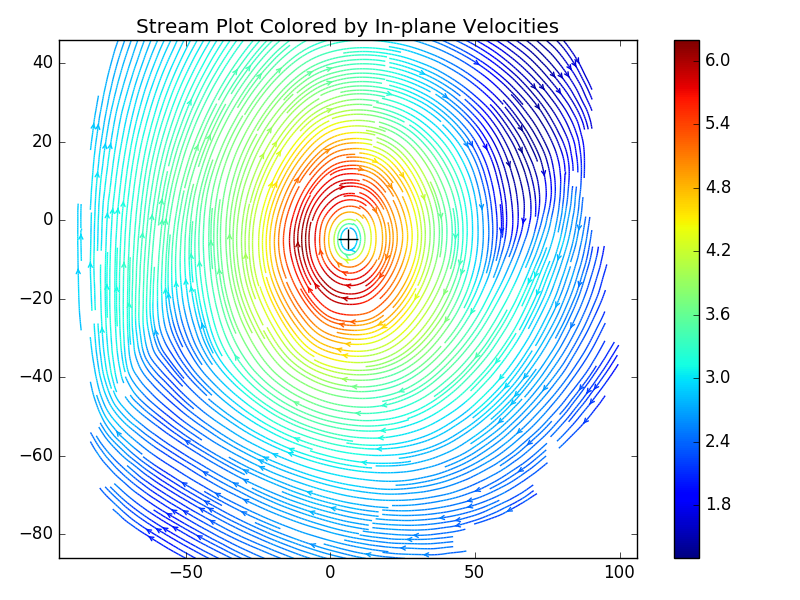
\includegraphics[width=5in]{figs/example_vortex_figs/example_stream}
	\caption{Example stream plot of run ID 55.}
	\label{fig:examp_stream}
\end{figure}

\begin{figure}[H]
	\centering
	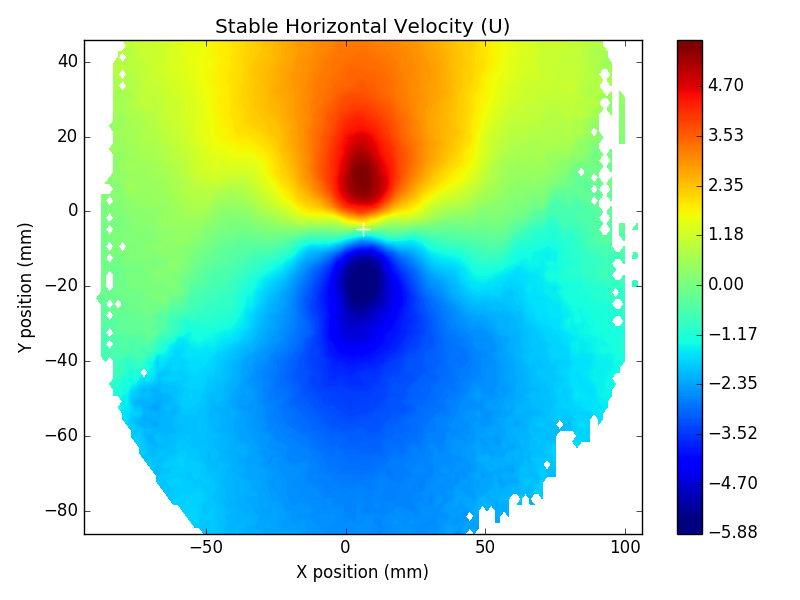
\includegraphics[width=5in]{figs/example_vortex_figs/example_U_contour}
\caption{Example contour plot of $\overline{u}$ for run ID 55.}
\label{fig:examp_U}
\end{figure}

\begin{figure}[H]
	\centering
	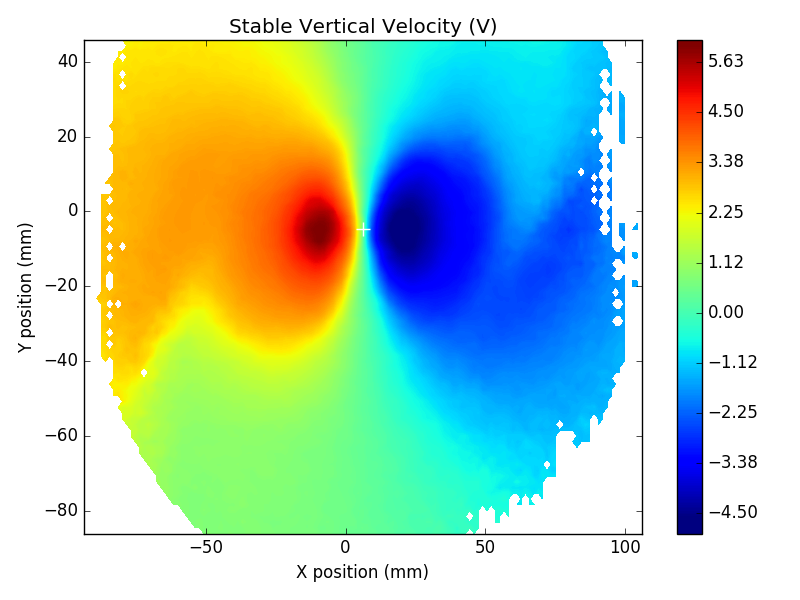
\includegraphics[width=5in]{figs/example_vortex_figs/example_V_contour}
\caption{Example contour plot of $\overline{v}$ for run ID 55.}
\label{fig:examp_V}
\end{figure}

\begin{figure}[H]
	\centering
	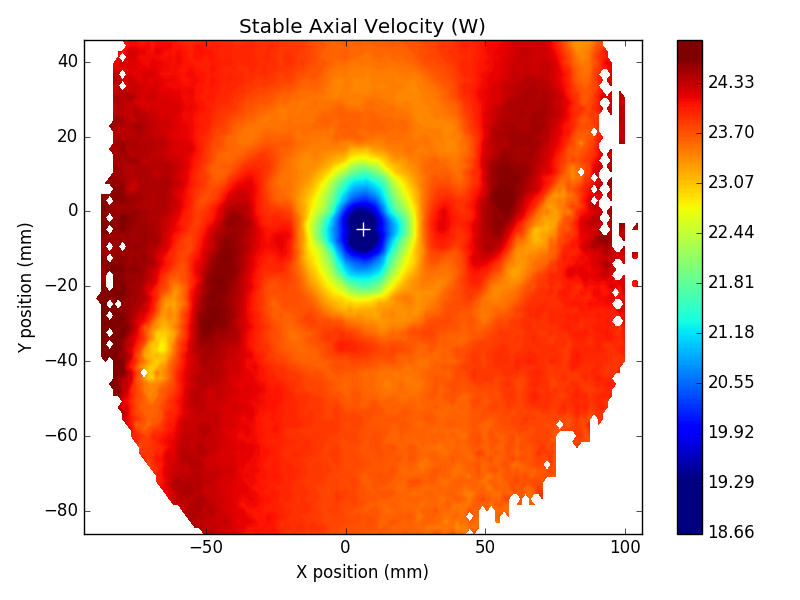
\includegraphics[width=5in]{figs/example_vortex_figs/example_W_contour}
\caption{Example contour plot of $\overline{w}$ for run ID 55.}
\label{fig:examp_W}
\end{figure}

\begin{figure}[H]
	\centering
	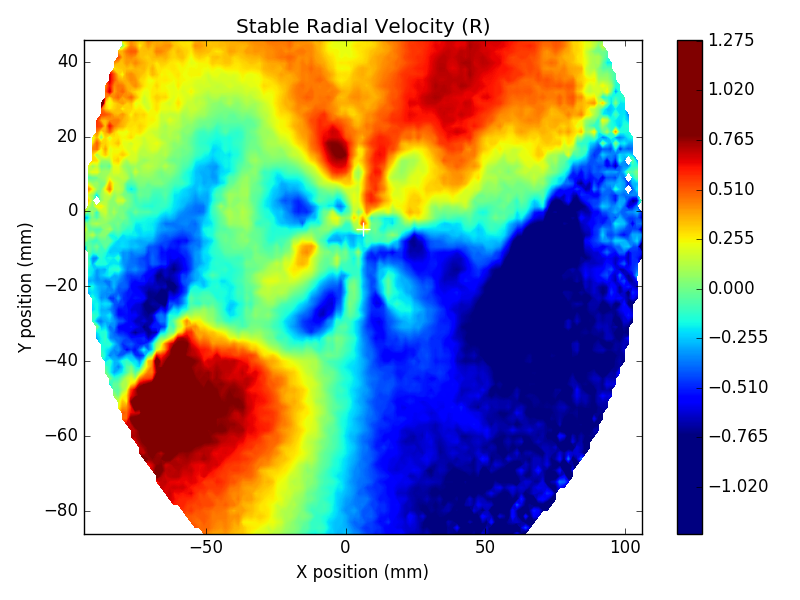
\includegraphics[width=5in]{figs/example_vortex_figs/example_R_contour}
\caption{Example contour plot of $\overline{r}$ for run ID 55.}
\label{fig:examp_R}
\end{figure}

\begin{figure}[H]
	\centering
	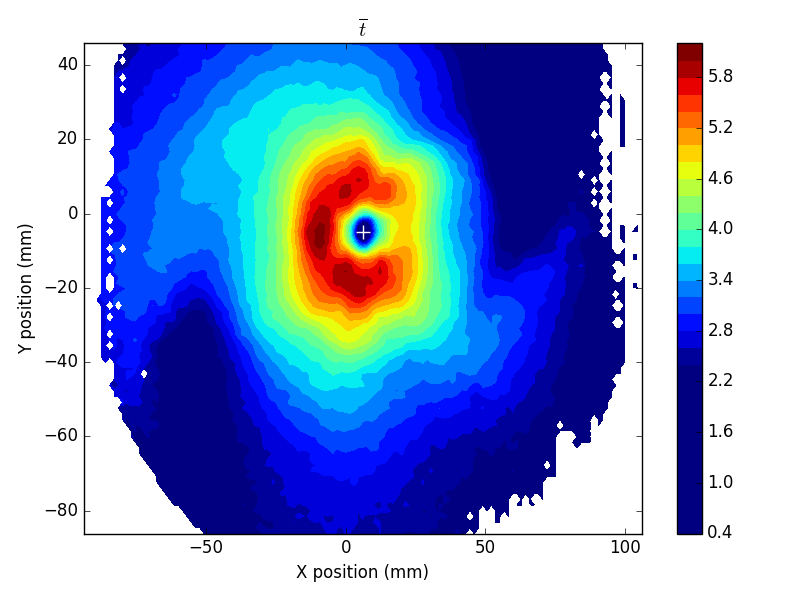
\includegraphics[width=5in]{figs/example_vortex_figs/example_T_contour}
\caption{Example contour plot of $\overline{t}$ for run ID 55.}
\label{fig:examp_T}
\end{figure}

\begin{figure}[H]
	\centering
	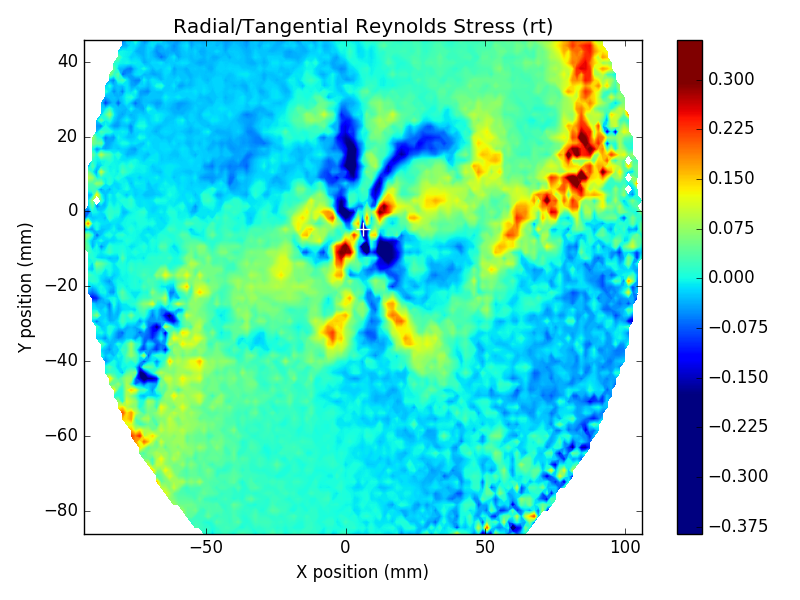
\includegraphics[width=5in]{figs/example_vortex_figs/example_rt_contour}
\caption{Example contour plot of $\overline{r^\prime t^\prime}$ for run ID 55.}
\label{fig:examp_rt}
\end{figure}

\begin{figure}[H]
	\centering
	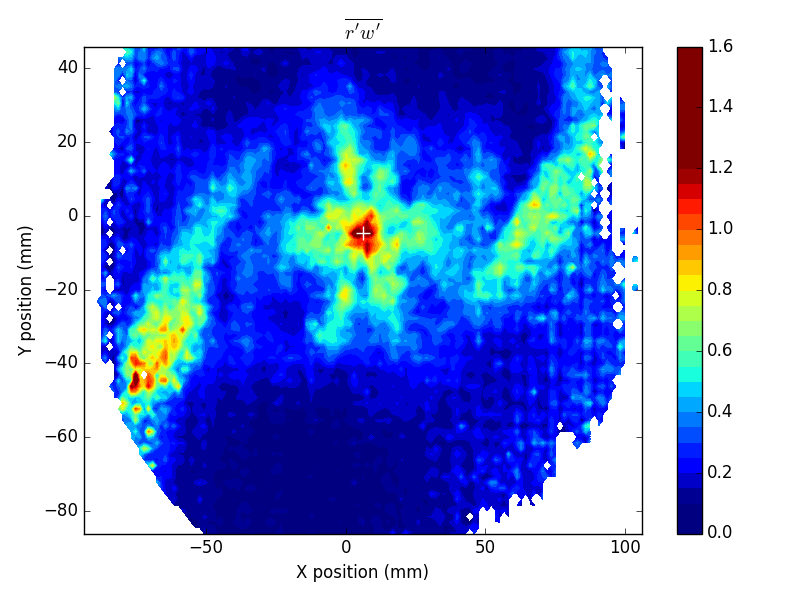
\includegraphics[width=5in]{figs/example_vortex_figs/example_rw_contour}
\caption{Example contour plot of $\overline{r^\prime w^\prime}$ for run ID 55.}
\label{fig:examp_rw}
\end{figure}

\begin{figure}[H]
	\centering
	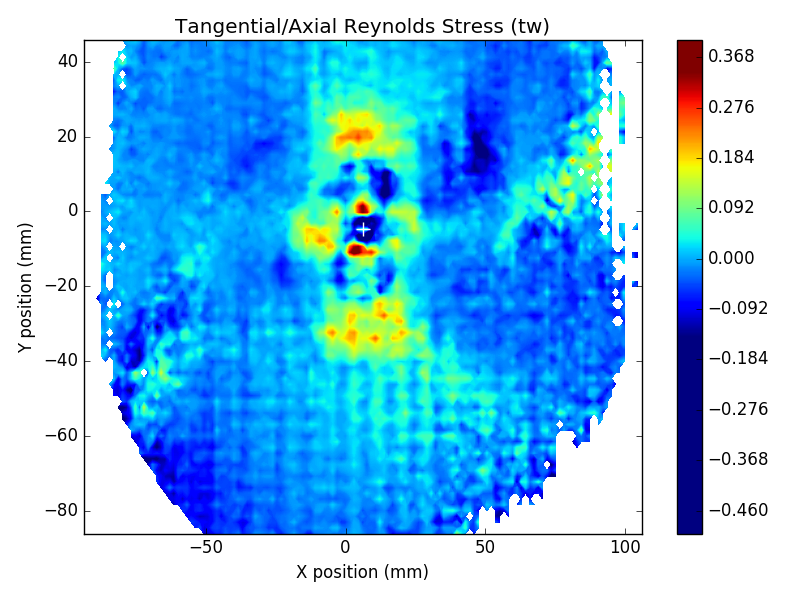
\includegraphics[width=5in]{figs/example_vortex_figs/example_tw_contour}
\caption{Example contour plot of $\overline{t^\prime w^\prime}$ for run ID 55.}
\label{fig:examp_tw}
\end{figure}

\begin{figure}[H]
	\centering
	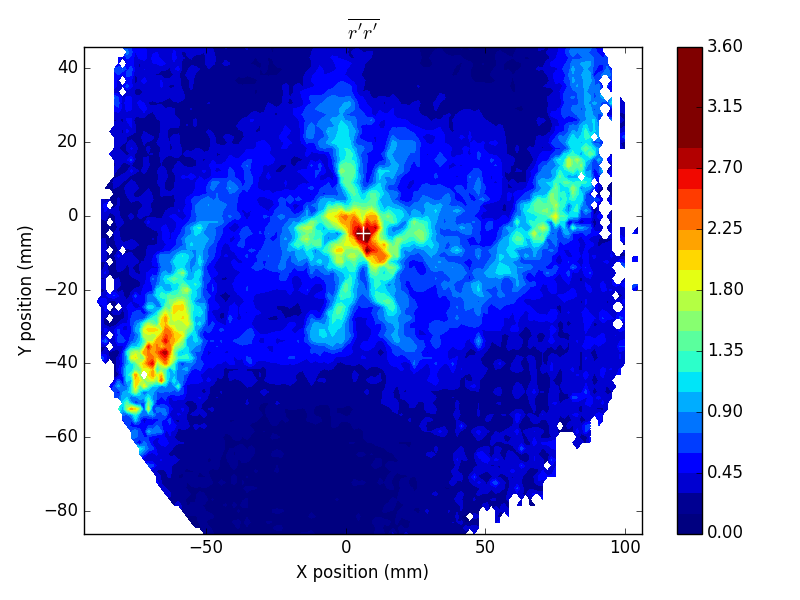
\includegraphics[width=5in]{figs/example_vortex_figs/example_rr_contour}
\caption{Example contour plot of $\overline{r^\prime r^\prime}$ for run ID 55.}
\label{fig:examp_rr}
\end{figure}

\begin{figure}[H]
	\centering
	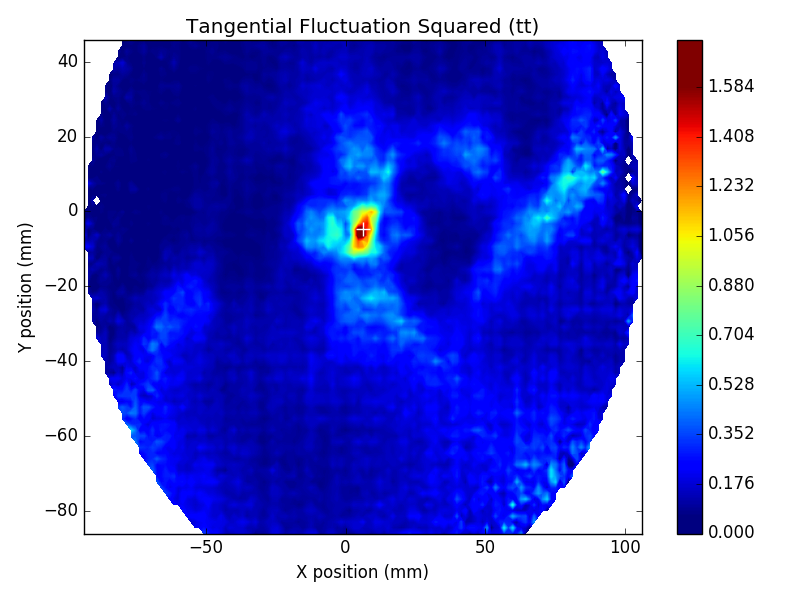
\includegraphics[width=5in]{figs/example_vortex_figs/example_tt_contour}
\caption{Example contour plot of $\overline{t^\prime t^\prime}$ for run ID 55.}
\label{fig:examp_tt}
\end{figure}

\begin{figure}[H]
	\centering
	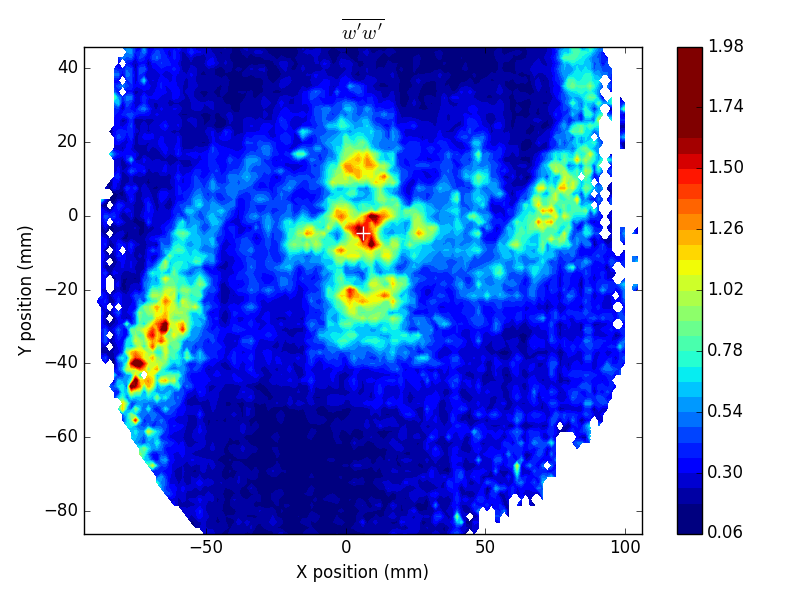
\includegraphics[width=5in]{figs/example_vortex_figs/example_ww_contour}
\caption{Example contour plot of $\overline{w^\prime w^\prime}$ for run ID 55.}
\label{fig:examp_ww}
\end{figure}

\begin{figure}[H]
	\centering
	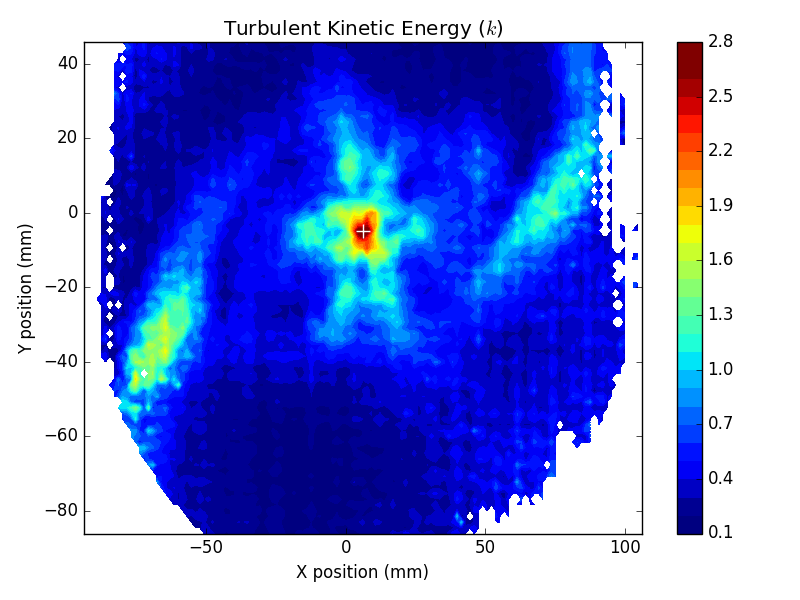
\includegraphics[width=5in]{figs/example_vortex_figs/example_ctke_contour}
\caption{Example contour plot of turbulent kinetic energy $k$ for run ID 55.}
\label{fig:examp_tke}
\end{figure}

\begin{figure}[H]
	\centering
	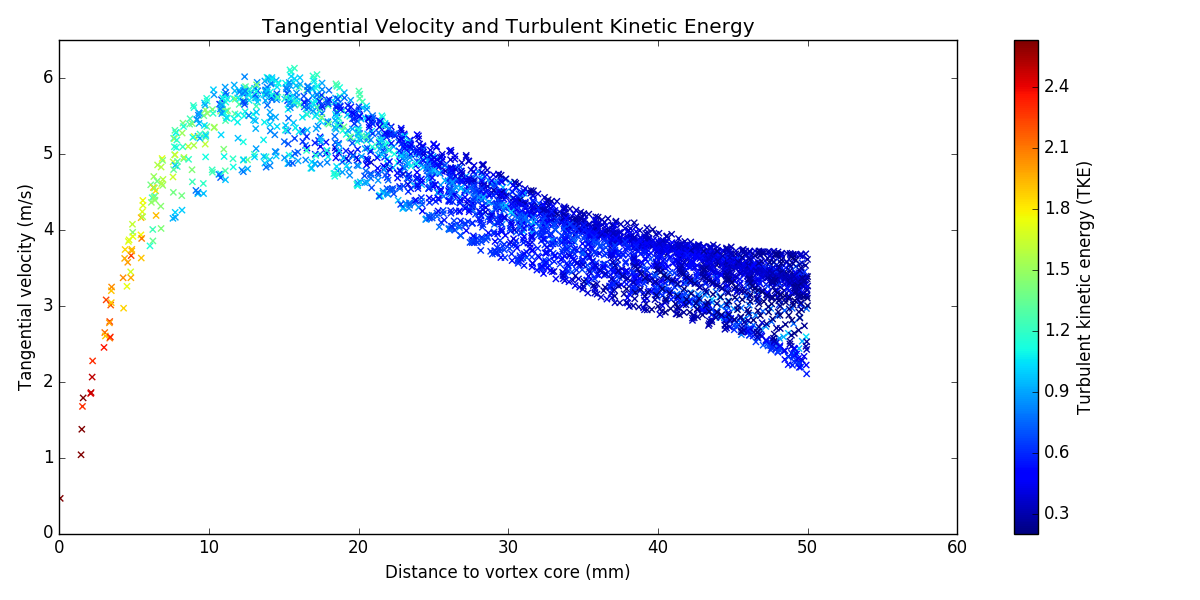
\includegraphics[width=7in]{figs/example_vortex_figs/example_TscatterTKE}
\caption{Example scatter plot of $T$, colored by $k$ for run ID 55.}
\label{fig:examp_Tscatter}
\end{figure}

Insight to the quality and uncertainty in each measurement was gained by 
examining the number of vectors successfully extracted from the set of 200 
snapshots as shown in Figure \ref{fig:example_num_contour}. Locations with 
fewer than twenty valid vectors in the set of 200 were thrown out. A clear 
relationship between the total turbulent kinetic energy, $k$, and the number of 
vectors making up the average was observed, and is discussed in Chapter 3.

\begin{figure}[H]
	\centering
	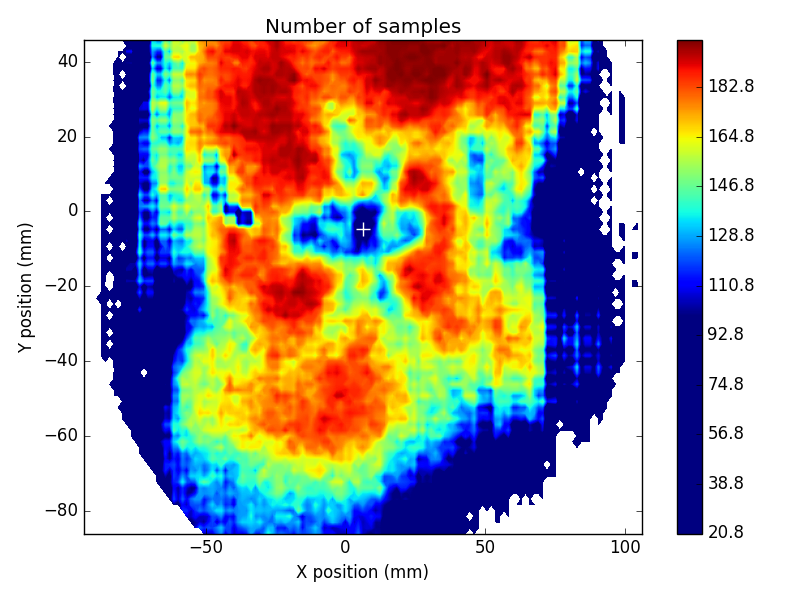
\includegraphics[width=5in]{figs/example_vortex_figs/example_num_contour}
	\caption{Example contour plot showing the variation in the number of 
	measurements within the interrogation plane}
	\label{fig:example_num_contour}
\end{figure}

\fi
%=========================================================================
\iftrue		% set to \iftrue to print to the next \fi, \iffalse not to
\chapter{Experiment Results}
\label{chapter:results}

\section{Discussion}

flag
\section{Uncertainty in PIV measurements}
\label{sec:piv_uncert}
 
There are a number of factors that contribute to uncertainty in PIV 
measurements. Both bias and precision errors can be estimated by considering 
detailed information about the optical geometry of the PIV setup. Monte Carlo 
based error estimation techniques can be applied by creating artificially 
simulated images with randomly distributed particles \cite{adeyinka2005}. 
The distribution of these particles can be modeled using a Gaussian intensity  
profile by (flag, reference) as described in Equation 
\ref{eq:piv_gaussian_uncertainty}.

\begin{equation}
	I(x,y) = I_0exp \left( \frac{-(x_{img} - x_p)^2 - (y_{img} - y_p)^2}
	{\frac{1}{8}d_\tau^2} \right)
	\label{eq:piv_gaussian_uncertainty}
\end{equation}
%
Where $x_p$ and $y_p$ are the locations of the particle centroid, $d_\tau$ is 
the diameter of of the particle, and $I_0$ is particle intensity. Particle 
intensity is directly related to the intensity of the light sheet, which is 
modeled as a Gaussian distribution \cite{PIVuncertAIAA}. This assumption allows 
us 
to express particle intensity as \ref{eq:particle_intensity_gaus}

\begin{equation}
	I_0(z_p) = (q)exp\left(- \frac{z_p^2}{\frac{1}{8}\Delta Z_L^2}\right)
	\label{eq:particle_intensity_gaus}
\end{equation}
%
Where $z_p$ is the particles position within the thickness of the light sheet, 
$q$ is the particle light scattering efficiency, and $\Delta Z_L$ is the 
thickness of the light sheet.

These formula are used to generate artificial image pairs for a single camera. 
A sufficient number of particles are created with $x$, $y$ and $z$ coordinates 
to meet particle density parameters, these coordinates are then 
used to generate light intensities according to Equation 
\ref{eq:particle_intensity_gaus}, which populate the image plane of the first 
image $A$. Next, a displacement image, $B$, is generated by shifting all the 
particles in a predetermined direction in three dimensional space. It is worth 
noting that for a single camera setup, particle movements in the $z$ direction 
do not produce pixel displacements, but simply determine the intensity of the 
light reflected from the particle. The known particle displacements can then be 
compared against outputs calculated with PIV capture and processing software.

To translate this concept to stereo PIV, an additional step is required. 
Instead of directly placing particles with known coordinates onto the image 
plane of one camera, they are placed on a conceptual version of the 
interrogation plane. The coordinate transforms obtained from PIV calibration 
are used to map the displacements from the conceptual plane into the image 
plane of each camera. These coordinate transforms are unique to each camera, 
and depend upon the optical geometry of the PIV setup. Uncertainty is 
calculated using the recommended AIAA calibration procedure outlined in 
\cite{PIVuncertAIAA}. To determine the system bias, the mean difference between 
the velocity standard established by the Monte Carlo simulation and the 
velocity calculated by the PIV software are compared as follows

\begin{equation}
\overline{\Delta U} = \frac{1}{N} \left(\sum_{i=1}^N \Delta U_i \right),
\label{eq:Uerror}
\end{equation}

\begin{equation}
\overline{\Delta V} = \frac{1}{N} \left(\sum_{i=1}^N \Delta V_i \right),
\label{eq:Verror}
\end{equation}

\begin{equation}
\overline{\Delta W} = \frac{1}{N} \left(\sum_{i=1}^N \Delta W_i \right)
\label{eq:Werror}
\end{equation}
%
Which is simply the average difference between the known velocity components 
and the measured velocity components $\Delta U$, $\Delta V$, and $\Delta W$ for 
a large number of simulations. This is referred to as the bias, and the three 
bias components are denoted as

\begin{equation}
\beta_{U} = \overline{\Delta U}
\label{eq:Ubias}
\end{equation}
\begin{equation}
\beta_{V} = \overline{\Delta V}
\label{eq:Vbias}
\end{equation}
\begin{equation}
\beta_{W} = \overline{\Delta W}
\label{eq:Wbias}
\end{equation}

The measurement precision is reported as the root-mean-square of the  
standard deviation, calculated as in 
	
\begin{equation}
S_{\Delta U} = \sqrt{\frac{1}{N-1} \left(\sum_{i=1}^N (\Delta U_i - 
\overline{\Delta U})^2 \right)}
\label{eq:Usd}
\end{equation}

\begin{equation}
S_{\Delta V} = \sqrt{\frac{1}{N-1} \left(\sum_{i=1}^N (\Delta V_i - 
	\overline{\Delta V})^2 \right)}
\label{eq:Vsd}
\end{equation}

\begin{equation}
S_{\Delta W} = \sqrt{\frac{1}{N-1} \left(\sum_{i=1}^N (\Delta W_i - 
	\overline{\Delta W})^2 \right)}
\label{eq:Wsd}
\end{equation}
%
Resulting in precision calculations given by 
%	
\begin{equation}
P_{\overline{U}} = \frac{2 S_{\Delta U}}{\sqrt{N}}
\label{eq:Uprec}
\end{equation}

\begin{equation}
P_{\overline{V}} = \frac{2 S_{\Delta V}}{\sqrt{N}}
\label{eq:Vprec}
\end{equation}

\begin{equation}
P_{\overline{W}} = \frac{2 S_{\Delta W}}{\sqrt{N}}
\label{eq:Wprec}
\end{equation}

Total uncertainty for each component at the 95\% confidence level is calculated 
by combining the bias and precision via to obtain

\begin{equation}
U_{\overline{\Delta U}} = \sqrt{\beta_{U}^2 + P_{\overline{U}}^2}
\label{eq:Uuncert}
\end{equation}
\begin{equation}
U_{\overline{\Delta V}} = \sqrt{\beta_{V}^2 + P_{\overline{V}}^2}
\label{eq:Vuncert}
\end{equation}
\begin{equation}
U_{\overline{\Delta W}} = \sqrt{\beta_{W}^2 + P_{\overline{W}}^2}
\label{eq:Wuncert}
\end{equation}


For these experiments, uncertainty analysis was conducted after the 
experimental data was taken. Vortices were characterized by velocities at key 
locations that allow each vortex to be described by one of the common vortex 
models. Characterization velocities of particular interest include the maximum 
tangential velocity about the vortex core, the distance of this high tangential 
velocity region from the core, which defined the core radius, and the typical 
axial velocity distribution near the free stream velocity. Understanding the 
uncertainty of these measurements required a Monte Carlo approach from 
synthetically created particle imagery. Artificial pixel displacements were 
specified to approximate the typical displacement associated with the 
velocities of greatest interest. 

To add complexity, the time between frame captures, $dt$ was expected to have a 
significant impact on uncertainty. Since the range of velocities used in this 
study required the use of multiple values of $dt$, artificial images were 
generated for a scenario at each value of $dt$ and the associated velocities. 
With the exception of measurements at station one, the furthest upstream 
observations at $I_Z$ of 546$mm$ down stream, all tests were conducted with a 
$dt$ value of 25, or 40 $\mu s$. At station one $dt$ values of 35 were also 
used. During the experimentation period, great difficulty 
was encountered in tuning PIV parameters to achieve well resolved vector fields 
at station one. The uncertainty analysis will demonstrate that the geometry of 
viewing angles was also unfavorable at this station, and the quality of 
measurements taken this far upstream was poor, they were therefore entirely 
disregarded. 

Creation of these artificial images by Monte Carlo was performed with custom 
software written in Python. This software parses the calibration files output 
from INSIGHT software and constructs the set of equations needed for all 
coordinate transformations. In order to simulate as accurately as possible, 
artificial images were generated at the full resolution of the PIV cameras 
used, (1280 x 1024). Particles were only generated randomly at coordinates 
that were within the field of view of both cameras, to eliminate wasted 
computation time generating particles which would not aid in the production of 
a three dimensional vector. An excess of 100,000 particles were simulated for 
each image set in order to ensure particle density was sufficient to resolve a 
vector in the majority of all sectors, and to match the experimental seed 
density as closely as possible. The most accurate way to ensure the intensities 
of each particle are accurately represented is to evaluate the intensity for 
every particle every point in the full image space of 1280 x 1024 pixels, and 
then add them together. Since this produces a three dimensional space in excess 
of a five billion values for a set of $La, Lb, Ra$ and $Rb$ images, computation 
time for uncertainty images was a limiting factor. At minimum, one set of 
uncertainty images for each combination of viewing geometry and time step $dt$ 
was required. Therefore, simulated velocity values were chosen for each of the 
14 cases to approximate the velocities of greatest interest. 

Tables \ref{table:experiment_results_1} through 
\ref{table:experiment_results_7} show a summary of results from each of the 70 
tests conducted, including the maximum 
observed azimuthal velocity, the average measured axial velocity, and the low 
axial velocity at the vortex core. At the three furthest positions downstream 
where the vortex appears to have stabilized, the typical value of maximum 
tangential velocity, $\overline{t}_{max}$ in component notation, ranges from 
6.0 to 7.9 $m/s$ for each run with a $dt$ of $25 \mu s$. This tangential 
velocity could align with the $X$ or the $Y$ axis, and 
it was desirable to simulate displacements in both directions at once to limit 
the number of Monte Carlo tests to be performed, so simulated velocities
$\overline{u}_{sim}$ and $\overline{v}_{sim}$
of $4.9 m/s$ was used such that the in-plane magnitude would be equal 
to the the middle of this range. Likewise, a simulated $\overline{u}_{sim}$ and 
$\overline{v}_{sim}$  velocity of 
$3.3 m/s$ was used to create synthetic images for testing experiments with a 
$dt$ of $40 \mu s$. In the axial direction, $Z$ , mean values $19 m/s$ and $29 
m/s$ were used for the high and low velocity experiments respectively. of These 
conditions are summarized in Table \ref{table:uncertainty_sim_table}.

\begin{table}[H]
\begin{center}
\begin{tabular}{|ccccc|}
	\hline
	Applies to & $dt$ & $\overline{u}_{sim}$ & $\overline{v}_{sim}$ & $\overline{w}_{sim}$\\
	  & $\mu s$ & $m/s$ & $m/s$ & $m/s$\\
	\hline
	Experiments where $V_{fs} < 24 m/s$ & 40 & 3.3 & 3.3 & 16\\
	Experiments where $V_{fs} > 24 m/s$ & 25 & 4.9 & 4.9 & 24\\
	\hline
\end{tabular}
\caption{Velocity conditions of Monte Carlo image generation for uncertainty analysis.}
\label{table:uncertainty_sim_table}
\end{center}
\end{table}


Even though many samples were taken at every vector location, the uncertainty 
in each individual measurement was of great importance for studying the 
unstable component of the velocity, and thus turbulent phenomena. Uncertainty 
in the fluctuating component were best represented by using an $N$ 
value of one in precision Equations \ref{eq:Uprec} through \ref{eq:Wprec}. 
Uncertainty in the stable component was lower, since this measurement is a 
result of averaging many measurements, and was calculated by using an $N$ value 
of 200 in the precision Equations \ref{eq:Uprec} through \ref{eq:Wprec}.


\subsection{Uncertainty Analysis Results}
The Monte Carlo analysis was performed for each station at two scenarios. 
Uncertainty in the measurements by $u, v$ and $w$ 
components are tabulated in Tables \ref{table:uncertainties_u} through 
\ref{table:uncertainties_w}. For the $u$ velocity components in the $X$ 
direction, the measurement is $\bar{u}$, bias are reported as $\beta_u$, 
precisions are reported for both single sample measurements and with 
measurements comprised of 200 averages by $P_{u^\prime}$ and $P_{\bar{u}}$ 
respectively, and total uncertainties are reported as $U_{u^\prime}$ and 
$U_{\bar{u}}$. 

\renewcommand\baselinestretch{1.3}\selectfont
\begin{table}[H]
\begin{center}
\begin{tabular}{|ccccccccccc|}
	\hline
	Station & $dt$ & $u_{sim}$ & $v_{sim}$ & $w_{sim}$ & $\bar{u}$ & $\beta_u$ & $P_{u^{\prime}}$ & $P_{\bar{u}}$ & $U_{u^{\prime}}$ & $U_{\bar{u}}$\\
	\hline
	1 & 25 & 6.15 & 6.15 & 24.0 & 6.756 & 0.606 & 1.883 & 0.133 & 1.978 & 0.620\\
	1 & 40 & 5.6 & 5.6 & 16.0 & 5.759 & 0.159 & 0.717 & 0.051 & 0.735 & 0.167\\
	2 & 25 & 6.15 & 6.15 & 24.0 & 6.247 & 0.097 & 2.480 & 0.175 & 2.482 & 0.201\\
	2 & 40 & 5.6 & 5.6 & 16.0 & 5.557 & -0.043 & 1.300 & 0.092 & 1.301 & 0.101\\
	3 & 25 & 6.15 & 6.15 & 24.0 & 5.492 & -0.658 & 1.282 & 0.091 & 1.442 & 0.665\\
	3 & 40 & 5.6 & 5.6 & 16.0 & 5.588 & -0.012 & 1.354 & 0.096 & 1.354 & 0.097\\
	4 & 25 & 6.15 & 6.15 & 24.0 & 5.610 & -0.540 & 0.975 & 0.069 & 1.114 & 0.544\\
	4 & 40 & 5.6 & 5.6 & 16.0 & 5.696 & 0.096 & 0.844 & 0.060 & 0.849 & 0.113\\
	5 & 25 & 6.15 & 6.15 & 24.0 & 6.579 & 0.429 & 1.608 & 0.114 & 1.664 & 0.444\\
	5 & 40 & 5.6 & 5.6 & 16.0 & 5.917 & 0.317 & 0.667 & 0.047 & 0.738 & 0.321\\
	6 & 25 & 6.15 & 6.15 & 24.0 & 7.366 & 1.216 & 1.463 & 0.103 & 1.902 & 1.220\\
	6 & 40 & 5.6 & 5.6 & 16.0 & 5.841 & 0.241 & 0.595 & 0.042 & 0.642 & 0.245\\
	7 & 25 & 6.15 & 6.15 & 24.0 & 6.972 & 0.822 & 1.885 & 0.133 & 2.056 & 0.832\\
	7 & 40 & 5.6 & 5.6 & 16.0 & 5.688 & 0.088 & 1.014 & 0.072 & 1.018 & 0.114\\
	\hline
\end{tabular}
\caption{Uncertainty in $X$ direction velocity measurements. Unlabelled units are $m/s$.}
\label{table:uncertainties_u}
\end{center}
\end{table}
\renewcommand\baselinestretch{2}\selectfont

\renewcommand\baselinestretch{1.3}\selectfont
\begin{table}[H]
\begin{center}
\begin{tabular}{|ccccccccccc|}
	\hline
	Station & $dt$ & $u_{sim}$ & $v_{sim}$ & $w_{sim}$ & $\bar{v}$ & $\beta_v$ & $P_{v^{\prime}}$ & $P_{\bar{v}}$ & $U_{v^{\prime}}$ & $U_{\bar{v}}$\\
	\hline
	1 & 25 & 6.15 & 6.15 & 24.0 & 5.155 & -0.995 & 0.717 & 0.051 & 1.226 & 0.996\\
	1 & 40 & 5.6 & 5.6 & 16.0 & 4.159 & -1.441 & 0.444 & 0.031 & 1.508 & 1.441\\
	2 & 25 & 6.15 & 6.15 & 24.0 & 5.597 & -0.553 & 0.615 & 0.044 & 0.827 & 0.554\\
	2 & 40 & 5.6 & 5.6 & 16.0 & 4.805 & -0.795 & 0.744 & 0.053 & 1.089 & 0.797\\
	3 & 25 & 6.15 & 6.15 & 24.0 & 5.530 & -0.620 & 0.545 & 0.039 & 0.825 & 0.621\\
	3 & 40 & 5.6 & 5.6 & 16.0 & 4.790 & -0.810 & 0.538 & 0.038 & 0.973 & 0.811\\
	4 & 25 & 6.15 & 6.15 & 24.0 & 5.585 & -0.565 & 0.588 & 0.042 & 0.815 & 0.567\\
	4 & 40 & 5.6 & 5.6 & 16.0 & 4.902 & -0.698 & 0.537 & 0.038 & 0.881 & 0.699\\
	5 & 25 & 6.15 & 6.15 & 24.0 & 5.729 & -0.421 & 0.623 & 0.044 & 0.752 & 0.424\\
	5 & 40 & 5.6 & 5.6 & 16.0 & 5.153 & -0.447 & 0.510 & 0.036 & 0.679 & 0.449\\
	6 & 25 & 6.15 & 6.15 & 24.0 & 5.832 & -0.318 & 0.744 & 0.053 & 0.809 & 0.322\\
	6 & 40 & 5.6 & 5.6 & 16.0 & 5.301 & -0.299 & 0.534 & 0.038 & 0.612 & 0.301\\
	7 & 25 & 6.15 & 6.15 & 24.0 & 6.060 & -0.090 & 0.780 & 0.055 & 0.785 & 0.106\\
	7 & 40 & 5.6 & 5.6 & 16.0 & 5.579 & -0.021 & 0.633 & 0.045 & 0.633 & 0.050\\
	\hline
\end{tabular}
\caption{Uncertainty in $Y$ direction velocity measurements. Unlabelled units are $m/s$.}
\label{table:uncertainties_v}
\end{center}
\end{table}
\renewcommand\baselinestretch{2}\selectfont

\begin{table}[H]
\begin{center}
\begin{tabular}{|ccccccccccc|}
	\hline
	Station & $dt$ & $u_{sim}$ & $v_{sim}$ & $w_{sim}$ & $\bar{w}$ & $\beta_w$ & $P_{w^{\prime}}$ & $P_{\bar{w}}$ & $U_{w^{\prime}}$ & $U_{\bar{w}}$\\
	\hline
	1 & 25 & 4.900 & 4.900 & 29.000 & 18.598 & -10.402 & 0.770 & 0.054 & 10.431 & 10.402\\
	1 & 40 & 3.300 & 3.300 & 19.000 & 11.834 & -7.166 & 0.372 & 0.026 & 7.176 & 7.166\\
	2 & 25 & 4.900 & 4.900 & 29.000 & 19.882 & -9.118 & 0.663 & 0.047 & 9.142 & 9.118\\
	2 & 40 & 3.300 & 3.300 & 19.000 & 12.993 & -6.007 & 0.684 & 0.048 & 6.045 & 6.007\\
	3 & 25 & 4.900 & 4.900 & 29.000 & 22.271 & -6.729 & 1.752 & 0.124 & 6.954 & 6.730\\
	3 & 40 & 3.300 & 3.300 & 19.000 & 15.310 & -3.690 & 0.928 & 0.066 & 3.805 & 3.691\\
	4 & 25 & 4.900 & 4.900 & 29.000 & 25.811 & -3.189 & 0.948 & 0.067 & 3.327 & 3.189\\
	4 & 40 & 3.300 & 3.300 & 19.000 & 16.657 & -2.343 & 0.358 & 0.025 & 2.371 & 2.344\\
	5 & 25 & 4.900 & 4.900 & 29.000 & 26.704 & -2.296 & 0.562 & 0.040 & 2.364 & 2.297\\
	5 & 40 & 3.300 & 3.300 & 19.000 & 17.006 & -1.994 & 0.297 & 0.021 & 2.016 & 1.994\\
	6 & 25 & 4.900 & 4.900 & 29.000 & 27.204 & -1.796 & 0.503 & 0.036 & 1.865 & 1.796\\
	6 & 40 & 3.300 & 3.300 & 19.000 & 17.398 & -1.602 & 0.502 & 0.036 & 1.679 & 1.602\\
	7 & 25 & 4.900 & 4.900 & 29.000 & 28.094 & -0.906 & 0.953 & 0.067 & 1.314 & 0.908\\
	7 & 40 & 3.300 & 3.300 & 19.000 & 18.626 & -0.374 & 0.931 & 0.066 & 1.003 & 0.380\\
	\hline
\end{tabular}
\caption{Uncertainty in $Z$ direction velocity measurements. Unlabelled units are $m/s$.}
\label{table:uncertainties_w}
\end{center}
\end{table}


The results of the Monte Carlo analysis held some surprises. Uncertainties in 
the $X$ and $Y$ direction were comparable in some cases, while in others $Y$ 
uncertainties were half as high as those in $X$. At all velocities, poor 
precision in the individual measurements was the primary driver of total 
uncertainty, while high bias was the driver for uncertainties in the 
measurements comprised of time averages of 200 samples. Spectral analysis of 
the turbulence over the observation time is subject to the very high 
uncertainties associated with that of individual measurements. Time averaged 
velocities, and the derived Reynolds stresses are best characterized by the 
better precision offered by many samples. While 200 is nominally used as $N$, 
each grid point may have between 20 and 200 valid vectors making up the set, so 
some areas where vectors were less frequently resolved successfully may be 
characterized with greater uncertainty.

In the axial $Z$ direction, the PIV was found to have an extreme bias to 
underestimate velocities according to the Monte Carlo simulation. This bias 
starts at over 30\% at the closest station, and diminishes regularly with 
downstream position and decreasing velocity . However, experimental data shows 
axial velocity was consistently a few percent above free stream velocity 
measured in the wind tunnel by dynamic pressure as expected, as shown in Tables
\ref{table:experiment_results_1} through \ref{table:experiment_results_7}. 
Therefore, uncertainties in the $Z$ direction are overestimated by the 
technique. The stable component of Reynolds decomposition is heavily influenced 
by a high bias, but the fluctuating component is entirely sensitive to 
precision. The Reynolds stress and turbulence values which are great importance 
in this study included contributions of velocity fluctuations in the axial 
direction, which are not impacted by any bias that does exist. Experimental 
data was examined for possible misrepresentation of measurement uncertainty in 
the $X$ and $Y$ direction, but no statistically meaningful discrepancies were 
found.


\fi
%=========================================================================
\iftrue		% set to \iftrue to print to the next \fi, \iffalse not to
\chapter{Conclusions}

flag
\fi
%=========================================================================
% constructs the bibliography
\bibliographystyle{apalike}
\bibliography{bib/vortices,bib/other,bib/particles,bib/piv}

\begin{thebibliography}{99}
%This command adds some extra space in the table of contents
\addtocontents{toc}{\vspace*{12pt}}  

% adds an entry for the bibliography in the table of contents
\addcontentsline{toc}{chapter}{BIBLIOGRAPHY}  
\end{thebibliography}

%=========================================================================

\appendix


\tocless\chapter{}
\section{Measurement Uncertainty}
\label{appendix:uncertainty_histograms}

This appendix shows histograms of measurements performed as part of the Monte 
Carlo uncertainty analysis.

\newpage
\tocless\section{Station 1}
\begin{figure}[H]
\centering
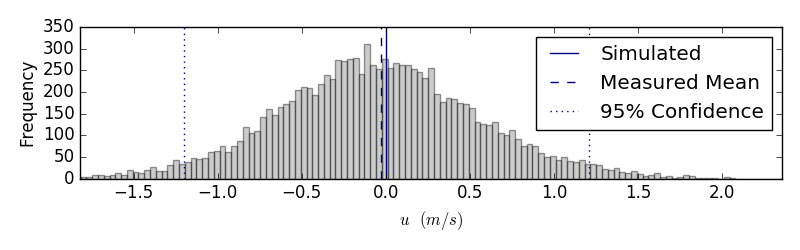
\includegraphics[width=6in]{figs/Ely_May28th01001/uncertainty_Ely_May28th01001_U}
\caption{Histogram of $U$ measurements at station 1. Simulated conditions $(u,v,w)=(6.15, 6.15, 24.0)$, $dt=25 \mu s$, $U_1_U=\pm 1.978$, $U_200_U=\pm 0.620$}
\label{fig:uncertainty_Ely_May28th01001_U}
\end{figure}


\begin{figure}[H]
\centering
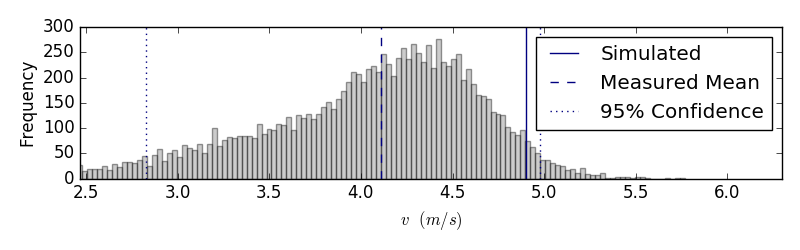
\includegraphics[width=6in]{figs/Ely_May28th01001/uncertainty_Ely_May28th01001_V}
\caption{Histogram of $V$ measurements at station 1. Simulated conditions $(u,v,w)=(6.15, 6.15, 24.0)$, $dt=25 \mu s$, $U_1_V=\pm 1.226$, $U_200_V=\pm 0.996$}
\label{fig:uncertainty_Ely_May28th01001_V}
\end{figure}


\begin{figure}[H]
\centering
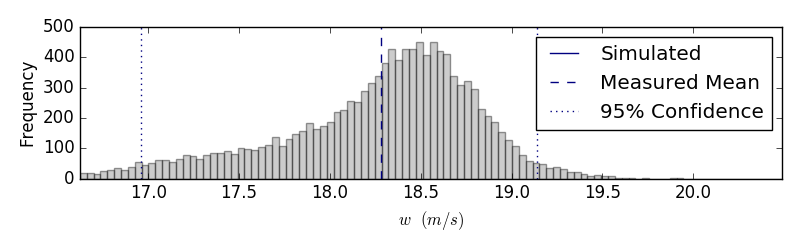
\includegraphics[width=6in]{figs/Ely_May28th01001/uncertainty_Ely_May28th01001_W}
\caption{Histogram of $W$ measurements at station 1. Simulated conditions $(u,v,w)=(6.15, 6.15, 24.0)$, $dt=25 \mu s$, $U_1_W=\pm 9.997$, $U_200_W=\pm 9.888$}
\label{fig:uncertainty_Ely_May28th01001_W}
\end{figure}



\begin{figure}[H]
\centering
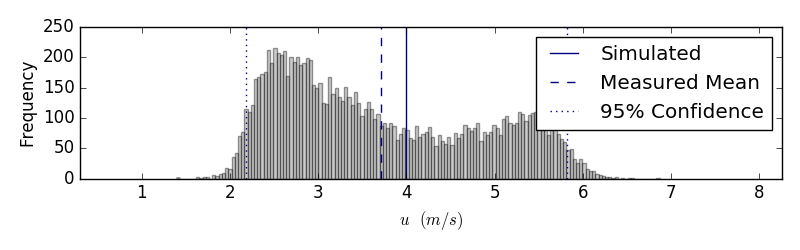
\includegraphics[width=6in]{figs/Ely_May28th01002/uncertainty_Ely_May28th01002_U}
\caption{Histogram of $U$ measurements at station 1. Simulated conditions $(u,v,w)=(3.3, 3.3, 19.0)$, $dt=40 \mu s$, $U_{1_{U}}=\pm 1.094$, $U_{200_{U}}=\pm 0.231$}
\label{fig:uncertainty_Ely_May28th01002_U}
\end{figure}


\begin{figure}[H]
\centering
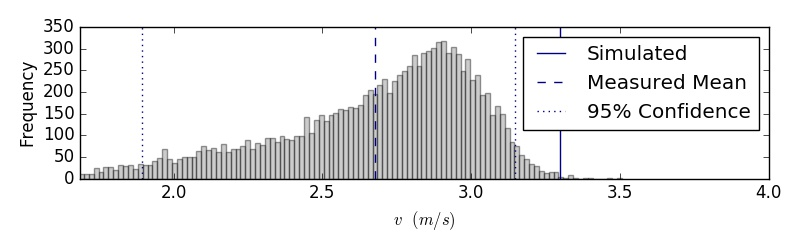
\includegraphics[width=6in]{figs/Ely_May28th01002/uncertainty_Ely_May28th01002_V}
\caption{Histogram of $V$ measurements at station 1. Simulated conditions $(u,v,w)=(3.3, 3.3, 19.0)$, $dt=40 \mu s$, $U_{1_{V}}=\pm 0.807$, $U_{200_{V}}=\pm 0.532$}
\label{fig:uncertainty_Ely_May28th01002_V}
\end{figure}


\begin{figure}[H]
\centering
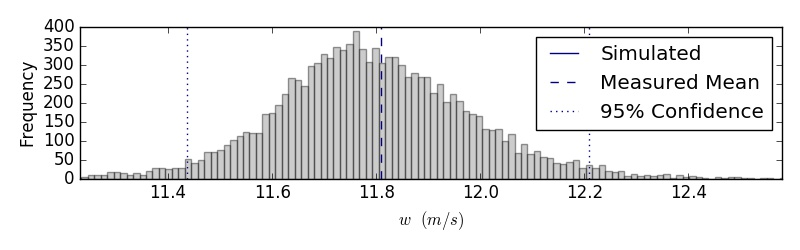
\includegraphics[width=6in]{figs/Ely_May28th01002/uncertainty_Ely_May28th01002_W}
\caption{Histogram of $W$ measurements at station 1. Simulated conditions $(u,v,w)=(3.3, 3.3, 19.0)$, $dt=40 \mu s$, $U_{1_{W}}=\pm 7.176$, $U_{200_{W}}=\pm 7.166$}
\label{fig:uncertainty_Ely_May28th01002_W}
\end{figure}




\tocless\section{Station 2}
\begin{figure}[H]
\centering
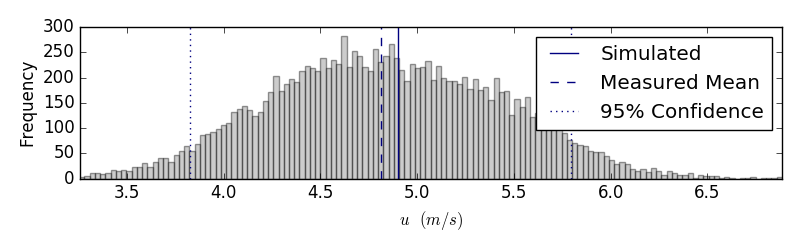
\includegraphics[width=6in]{figs/Ely_May28th02001/uncertainty_Ely_May28th02001_U}
\caption{Histogram of $U$ measurements at station 2. Simulated conditions $(u,v,w)=(4.9, 4.9, 29.0)$, $dt=25 \mu s$, $U_{1_{U}}=\pm 1.040$, $U_{200_{U}}=\pm 0.114$}
\label{fig:uncertainty_Ely_May28th02001_U}
\end{figure}


\begin{figure}[H]
\centering
\includegraphics[width=6in]{figs/Ely_May28th02001/uncertainty_Ely_May28th02001_V}
\caption{Histogram of $V$ measurements at station 2. Simulated conditions $(u,v,w)=(4.9, 4.9, 29.0)$, $dt=25 \mu s$, $U_{1_{V}}=\pm 0.733$, $U_{200_{V}}=\pm 0.084$}
\label{fig:uncertainty_Ely_May28th02001_V}
\end{figure}


\begin{figure}[H]
\centering
\includegraphics[width=6in]{figs/Ely_May28th02001/uncertainty_Ely_May28th02001_W}
\caption{Histogram of $W$ measurements at station 2. Simulated conditions $(u,v,w)=(4.9, 4.9, 29.0)$, $dt=25 \mu s$, $U_{1_{W}}=\pm 9.142$, $U_{200_{W}}=\pm 9.118$}
\label{fig:uncertainty_Ely_May28th02001_W}
\end{figure}



\begin{figure}[H]
\centering
\includegraphics[width=6in]{figs/Ely_May28th02002/uncertainty_Ely_May28th02002_U}
\caption{Histogram of $U$ measurements at station 2. Simulated conditions $(u,v,w)=(3.3, 3.3, 19.0)$, $dt=40 \mu s$, $U_1_U=\pm 0.957$, $U_200_U=\pm 0.100$}
\label{fig:uncertainty_Ely_May28th02002_U}
\end{figure}


\begin{figure}[H]
\centering
\includegraphics[width=6in]{figs/Ely_May28th02002/uncertainty_Ely_May28th02002_V}
\caption{Histogram of $V$ measurements at station 2. Simulated conditions $(u,v,w)=(3.3, 3.3, 19.0)$, $dt=40 \mu s$, $U_1_V=\pm 0.508$, $U_200_V=\pm 0.103$}
\label{fig:uncertainty_Ely_May28th02002_V}
\end{figure}


\begin{figure}[H]
\centering
\includegraphics[width=6in]{figs/Ely_May28th02002/uncertainty_Ely_May28th02002_W}
\caption{Histogram of $W$ measurements at station 2. Simulated conditions $(u,v,w)=(3.3, 3.3, 19.0)$, $dt=40 \mu s$, $U_1_W=\pm 6.045$, $U_200_W=\pm 6.007$}
\label{fig:uncertainty_Ely_May28th02002_W}
\end{figure}





%ensures every page has "Figure         Page" at the top of it
\makeatletter
\addtocontents{lof}{%
	\protect\afterpage{\protect\hbox to \linewidth%
		{\noindent Figure \hfill Page}\par%
		\protect\vspace{12\p@}}}
\makeatother


\tocless\section{Station 3}
\begin{figure}[H]
\centering
\includegraphics[width=6in]{figs/Ely_May28th03001/uncertainty_Ely_May28th03001_U}
\caption{Histogram of $U$ measurements at station 3. Simulated conditions $(u,v,w)=(4.9, 4.9, 29.0)$, $dt=25 \mu s$, $U_{1_{U}}=\pm 1.831$, $U_{200_{U}}=\pm 1.265$}
\label{fig:uncertainty_Ely_May28th03001_U}
\end{figure}


\begin{figure}[H]
\centering
\includegraphics[width=6in]{figs/Ely_May28th03001/uncertainty_Ely_May28th03001_V}
\caption{Histogram of $V$ measurements at station 3. Simulated conditions $(u,v,w)=(4.9, 4.9, 29.0)$, $dt=25 \mu s$, $U_{1_{V}}=\pm 2.086$, $U_{200_{V}}=\pm 2.023$}
\label{fig:uncertainty_Ely_May28th03001_V}
\end{figure}


\begin{figure}[H]
\centering
\includegraphics[width=6in]{figs/Ely_May28th03001/uncertainty_Ely_May28th03001_W}
\caption{Histogram of $W$ measurements at station 3. Simulated conditions $(u,v,w)=(4.9, 4.9, 29.0)$, $dt=25 \mu s$, $U_{1_{W}}=\pm 15.169$, $U_{200_{W}}=\pm 15.130$}
\label{fig:uncertainty_Ely_May28th03001_W}
\end{figure}



\begin{figure}[H]
\centering
\includegraphics[width=6in]{figs/Ely_May28th03002/uncertainty_Ely_May28th03002_U}
\caption{Histogram of $U$ measurements at station 3. Simulated conditions $(u,v,w)=(3.3, 3.3, 19.0)$, $dt=40 \mu s$, $U_{1_{U}}=\pm 1.881$, $U_{200_{U}}=\pm 0.648$}
\label{fig:uncertainty_Ely_May28th03002_U}
\end{figure}


\begin{figure}[H]
\centering
\includegraphics[width=6in]{figs/Ely_May28th03002/uncertainty_Ely_May28th03002_V}
\caption{Histogram of $V$ measurements at station 3. Simulated conditions $(u,v,w)=(3.3, 3.3, 19.0)$, $dt=40 \mu s$, $U_{1_{V}}=\pm 0.521$, $U_{200_{V}}=\pm 0.252$}
\label{fig:uncertainty_Ely_May28th03002_V}
\end{figure}


\begin{figure}[H]
\centering
\includegraphics[width=6in]{figs/Ely_May28th03002/uncertainty_Ely_May28th03002_W}
\caption{Histogram of $W$ measurements at station 3. Simulated conditions $(u,v,w)=(3.3, 3.3, 19.0)$, $dt=40 \mu s$, $U_{1_{W}}=\pm 3.881$, $U_{200_{W}}=\pm 3.762$}
\label{fig:uncertainty_Ely_May28th03002_W}
\end{figure}




\tocless\section{Station 4}
\begin{figure}[H]
\centering
\includegraphics[width=6in]{figs/Ely_May28th04001/uncertainty_Ely_May28th04001_U}
\caption{Histogram of $U$ measurements at station 4. Simulated conditions $(u,v,w)=(4.9, 4.9, 29.0)$, $dt=25 \mu s$, $U_{1_{U}}=\pm 2.252$, $U_{200_{U}}=\pm 1.856$}
\label{fig:uncertainty_Ely_May28th04001_U}
\end{figure}


\begin{figure}[H]
\centering
\includegraphics[width=6in]{figs/Ely_May28th04001/uncertainty_Ely_May28th04001_V}
\caption{Histogram of $V$ measurements at station 4. Simulated conditions $(u,v,w)=(4.9, 4.9, 29.0)$, $dt=25 \mu s$, $U_{1_{V}}=\pm 1.959$, $U_{200_{V}}=\pm 1.900$}
\label{fig:uncertainty_Ely_May28th04001_V}
\end{figure}


\begin{figure}[H]
\centering
\includegraphics[width=6in]{figs/Ely_May28th04001/uncertainty_Ely_May28th04001_W}
\caption{Histogram of $W$ measurements at station 4. Simulated conditions $(u,v,w)=(4.9, 4.9, 29.0)$, $dt=25 \mu s$, $U_{1_{W}}=\pm 12.931$, $U_{200_{W}}=\pm 12.914$}
\label{fig:uncertainty_Ely_May28th04001_W}
\end{figure}



\begin{figure}[H]
\centering
\includegraphics[width=6in]{figs/Ely_May28th04002/uncertainty_Ely_May28th04002_U}
\caption{Histogram of $U$ measurements at station 4. Simulated conditions 
$(u,v,w)=(3.3, 3.3, 19.0)$, $dt=40 \mu s$, $U_{1_{U}}=\pm 1.032$, 
$U_{200_{U}}=\pm 0.236$.}
\label{fig:uncertainty_Ely_May28th04002_U}
\end{figure}


\begin{figure}[H]
\centering
\includegraphics[width=6in]{figs/Ely_May28th04002/uncertainty_Ely_May28th04002_V}
\caption{Histogram of $V$ measurements at station 4. Simulated conditions 
$(u,v,w)=(3.3, 3.3, 19.0)$, $dt=40 \mu s$, $U_{1_{V}}=\pm 0.474$, 
$U_{200_{V}}=\pm 0.267$.}
\label{fig:uncertainty_Ely_May28th04002_V}
\end{figure}


\begin{figure}[H]
\centering
\includegraphics[width=6in]{figs/Ely_May28th04002/uncertainty_Ely_May28th04002_W}
\caption{Histogram of $W$ measurements at station 4. Simulated conditions 
$(u,v,w)=(3.3, 3.3, 19.0)$, $dt=40 \mu s$, $U_{1_{W}}=\pm 2.371$, 
$U_{200_{W}}=\pm 2.344$.}
\label{fig:uncertainty_Ely_May28th04002_W}
\end{figure}




%ensures every page has "Figure         Page" at the top of it
\makeatletter
\addtocontents{lof}{%
	\protect\afterpage{\protect\hbox to \linewidth%
		{\noindent Figure \hfill Page}\par%
		\protect\vspace{12\p@}}}
\makeatother


\tocless\section{Station 5}
\begin{figure}[H]
\centering
\includegraphics[width=6in]{figs/Ely_May28th05001/uncertainty_Ely_May28th05001_U}
\caption{Histogram of $U$ measurements at station 5. Simulated conditions $(u,v,w)=(0.0, 0.0, 5.0)$, $dt=40 \mu s$, $\beta_U=\pm -0.0185$, $P_U=\pm 0.1930$, $U_U=\pm 0.3865$}
\label{fig:uncertainty_Ely_May28th05001_U}
\end{figure}


\begin{figure}[H]
\centering
\includegraphics[width=6in]{figs/Ely_May28th05001/uncertainty_Ely_May28th05001_V}
\caption{Histogram of $V$ measurements at station 5. Simulated conditions $(u,v,w)=(0.0, 0.0, 5.0)$, $dt=40 \mu s$, $\beta_V=\pm -0.0285$, $P_V=\pm 0.1290$, $U_V=\pm 0.2596$}
\label{fig:uncertainty_Ely_May28th05001_V}
\end{figure}


\begin{figure}[H]
\centering
\includegraphics[width=6in]{figs/Ely_May28th05001/uncertainty_Ely_May28th05001_W}
\caption{Histogram of $W$ measurements at station 5. Simulated conditions $(u,v,w)=(0.0, 0.0, 5.0)$, $dt=40 \mu s$, $\beta_W=\pm -0.2765$, $P_W=\pm 0.1004$, $U_W=\pm 0.3417$}
\label{fig:uncertainty_Ely_May28th05001_W}
\end{figure}



\begin{figure}[H]
\centering
\includegraphics[width=6in]{figs/Ely_May28th05002/uncertainty_Ely_May28th05002_U}
\caption{Histogram of $U$ measurements at station 5. Simulated conditions $(u,v,w)=(3.3, 3.3, 19.0)$, $dt=40 \mu s$, $U_{1_{U}}=\pm 0.636$, $U_{200_{U}}=\pm 0.138$}
\label{fig:uncertainty_Ely_May28th05002_U}
\end{figure}


\begin{figure}[H]
\centering
\includegraphics[width=6in]{figs/Ely_May28th05002/uncertainty_Ely_May28th05002_V}
\caption{Histogram of $V$ measurements at station 5. Simulated conditions $(u,v,w)=(3.3, 3.3, 19.0)$, $dt=40 \mu s$, $U_{1_{V}}=\pm 0.317$, $U_{200_{V}}=\pm 0.039$}
\label{fig:uncertainty_Ely_May28th05002_V}
\end{figure}


\begin{figure}[H]
\centering
\includegraphics[width=6in]{figs/Ely_May28th05002/uncertainty_Ely_May28th05002_W}
\caption{Histogram of $W$ measurements at station 5. Simulated conditions $(u,v,w)=(3.3, 3.3, 19.0)$, $dt=40 \mu s$, $U_{1_{W}}=\pm 2.047$, $U_{200_{W}}=\pm 2.026$}
\label{fig:uncertainty_Ely_May28th05002_W}
\end{figure}




\tocless\section{Station 6}
\begin{figure}[H]
\centering
\includegraphics[width=6in]{figs/Ely_May28th06001/uncertainty_Ely_May28th06001_U}
\caption{Histogram of $U$ measurements at station 6. Simulated conditions $(u,v,w)=(0.0, 0.0, 5.0)$, $dt=40 \mu s$, $\beta_U=\pm -0.0133$, $P_U=\pm 0.1296$, $U_U=\pm 0.2596$}
\label{fig:uncertainty_Ely_May28th06001_U}
\end{figure}


\begin{figure}[H]
\centering
\includegraphics[width=6in]{figs/Ely_May28th06001/uncertainty_Ely_May28th06001_V}
\caption{Histogram of $V$ measurements at station 6. Simulated conditions $(u,v,w)=(0.0, 0.0, 5.0)$, $dt=40 \mu s$, $\beta_V=\pm -0.0225$, $P_V=\pm 0.0954$, $U_V=\pm 0.1921$}
\label{fig:uncertainty_Ely_May28th06001_V}
\end{figure}


\begin{figure}[H]
\centering
\includegraphics[width=6in]{figs/Ely_May28th06001/uncertainty_Ely_May28th06001_W}
\caption{Histogram of $W$ measurements at station 6. Simulated conditions $(u,v,w)=(0.0, 0.0, 5.0)$, $dt=40 \mu s$, $\beta_W=\pm -0.1734$, $P_W=\pm 0.0616$, $U_W=\pm 0.2128$}
\label{fig:uncertainty_Ely_May28th06001_W}
\end{figure}



\begin{figure}[H]
\centering
\includegraphics[width=6in]{figs/Ely_May28th06002/uncertainty_Ely_May28th06002_U}
\caption{Histogram of $U$ measurements at station 6. Simulated conditions $(u,v,w)=(5.6, 5.6, 16.0)$, $dt=40 \mu s$, $U_1_U=\pm 0.642$, $U_200_U=\pm 0.245$}
\label{fig:uncertainty_Ely_May28th06002_U}
\end{figure}


\begin{figure}[H]
\centering
\includegraphics[width=6in]{figs/Ely_May28th06002/uncertainty_Ely_May28th06002_V}
\caption{Histogram of $V$ measurements at station 6. Simulated conditions $(u,v,w)=(5.6, 5.6, 16.0)$, $dt=40 \mu s$, $U_1_V=\pm 0.612$, $U_200_V=\pm 0.301$}
\label{fig:uncertainty_Ely_May28th06002_V}
\end{figure}


\begin{figure}[H]
\centering
\includegraphics[width=6in]{figs/Ely_May28th06002/uncertainty_Ely_May28th06002_W}
\caption{Histogram of $W$ measurements at station 6. Simulated conditions $(u,v,w)=(5.6, 5.6, 16.0)$, $dt=40 \mu s$, $U_1_W=\pm 1.473$, $U_200_W=\pm 1.304$}
\label{fig:uncertainty_Ely_May28th06002_W}
\end{figure}




\tocless\section{Station 7}
\begin{figure}[H]
\centering
\includegraphics[width=6in]{figs/Ely_May28th07001/uncertainty_Ely_May28th07001_U}
\caption{Histogram of $U$ measurements at station 7. Simulated conditions $(u,v,w)=(6.15, 6.15, 29.0)$, $dt=25 \mu s$, $U_1_U=\pm 1.785$, $U_200_U=\pm 0.146$}
\label{fig:uncertainty_Ely_May28th07001_U}
\end{figure}


\begin{figure}[H]
\centering
\includegraphics[width=6in]{figs/Ely_May28th07001/uncertainty_Ely_May28th07001_V}
\caption{Histogram of $V$ measurements at station 7. Simulated conditions $(u,v,w)=(6.15, 6.15, 29.0)$, $dt=25 \mu s$, $U_1_V=\pm 0.709$, $U_200_V=\pm 0.054$}
\label{fig:uncertainty_Ely_May28th07001_V}
\end{figure}


\begin{figure}[H]
\centering
\includegraphics[width=6in]{figs/Ely_May28th07001/uncertainty_Ely_May28th07001_W}
\caption{Histogram of $W$ measurements at station 7. Simulated conditions $(u,v,w)=(6.15, 6.15, 29.0)$, $dt=25 \mu s$, $U_1_W=\pm 1.335$, $U_200_W=\pm 0.489$}
\label{fig:uncertainty_Ely_May28th07001_W}
\end{figure}



\begin{figure}[H]
\centering
\includegraphics[width=6in]{figs/Ely_May28th07002/uncertainty_Ely_May28th07002_U}
\caption{Histogram of $U$ measurements at station 7. Simulated conditions $(u,v,w)=(3.3, 3.3, 19.0)$, $dt=40 \mu s$, $U_1_U=\pm 1.560$, $U_200_U=\pm 0.332$}
\label{fig:uncertainty_Ely_May28th07002_U}
\end{figure}


\begin{figure}[H]
\centering
\includegraphics[width=6in]{figs/Ely_May28th07002/uncertainty_Ely_May28th07002_V}
\caption{Histogram of $V$ measurements at station 7. Simulated conditions $(u,v,w)=(3.3, 3.3, 19.0)$, $dt=40 \mu s$, $U_1_V=\pm 0.527$, $U_200_V=\pm 0.043$}
\label{fig:uncertainty_Ely_May28th07002_V}
\end{figure}


\begin{figure}[H]
\centering
\includegraphics[width=6in]{figs/Ely_May28th07002/uncertainty_Ely_May28th07002_W}
\caption{Histogram of $W$ measurements at station 7. Simulated conditions $(u,v,w)=(3.3, 3.3, 19.0)$, $dt=40 \mu s$, $U_1_W=\pm 1.003$, $U_200_W=\pm 0.380$}
\label{fig:uncertainty_Ely_May28th07002_W}
\end{figure}





%

\chapter{Station 1 PIV Data: 546mm Downstream}
\renewcommand\baselinestretch{1.3}\selectfont
\begin{table}[H]
\begin{center}
\begin{tabular}{|ccccccccccc|}
	\hline
	Run & $I_Z$ & $V_{nom}$ & $dt$ & $V_{fs}$ & $\sigma_{V_{fs}}$ & $Q$ & $P_{atm}$ & $T_{tunnel}$ & $\phi$ & $\eta_P$\\
	$ID$ & $(mm)$ & $(m/s)$ & $(\mu s)$ & $(m/s)$ & $(m/s)$ & $(Pa)$ & $(Pa)$ & $(\degree K)$ & $(\%)$ & $(\mu s)$\\
	\hline
	1 & 546 & 15 & 50 & 15.22 & 0.02 & 135 & 102036 & 299.85 & 60.4 & 0.35\\
	2 & 546 & 17 & 50 & 16.88 & 0.02 & 170 & 102115 & 297.55 & 66.3 & 0.329\\
	3 & 546 & 19 & 50 & 19.43 & 0.01 & 225 & 102105 & 297.55 & 66.3 & 0.329\\
	4 & 546 & 21 & 50 & 21.06 & 0.02 & 264 & 102100 & 297.75 & 66.3 & 0.324\\
	5 & 546 & 23 & 35 & 23.21 & 0.04 & 321 & 102097 & 297.95 & 66.3 & 0.324\\
	6 & 546 & 25 & 35 & 24.86 & 0.05 & 371 & 102093 & 298.15 & 66.3 & 0.324\\
	7 & 546 & 27 & 35 & 27.02 & 0.03 & 434 & 102092 & 298.3 & 66.3 & 0.324\\
	8 & 546 & 29 & 25 & 29.12 & 0.04 & 505 & 102080 & 298.35 & 66.3 & 0.324\\
	9 & 546 & 31 & 25 & 30.86 & 0.06 & 564 & 102050 & 299.15 & 66.3 & 0.324\\
	10 & 546 & 33 & 25 & 32.98 & 0.05 & 641 & 102054 & 299.9 & 60.4 & 0.35\\
	\hline
\end{tabular}
\caption{Experimental measurements for station 1}
\label{table:station_1_measurements}
\end{center}
\end{table}
\renewcommand\baselinestretch{2}\selectfont

\subsection{Run ID 1}
\begin{figure}[H]
\centering
\includegraphics[width=5in]{figs/appendix_run_id_1/appendix_run_id_1_stream}
\caption{Stream plot at $z/c$=5.37401574803, $V_{free}$=15.22, station 0.}
\label{fig:appendix_run_id_1_stream}
\end{figure}


\begin{figure}[H]
\centering
\includegraphics[width=5in]{figs/appendix_run_id_1/appendix_run_id_1_R__contour}
\caption{Contour plot of $\overline{r}$ at $z/c$=5.37401574803, $V_{free}$=15.22, station 0.}
\label{fig:appendix_run_id_1_R__contour}
\end{figure}


\begin{figure}[H]
\centering
\includegraphics[width=5in]{figs/appendix_run_id_1/appendix_run_id_1_T__contour}
\caption{Contour plot of $\overline{t}$ at $z/c$=5.37401574803, $V_{free}$=15.22, station 0.}
\label{fig:appendix_run_id_1_T__contour}
\end{figure}


\begin{figure}[H]
\centering
\includegraphics[width=5in]{figs/appendix_run_id_1/appendix_run_id_1_W__contour}
\caption{Contour plot of $\overline{w}$ at $z/c$=5.37401574803, $V_{free}$=15.22, station 0.}
\label{fig:appendix_run_id_1_W__contour}
\end{figure}


\begin{figure}[H]
\centering
\includegraphics[width=5in]{figs/appendix_run_id_1/appendix_run_id_1_rt__contour}
\caption{Contour plot of $\overline{r^\prime t^\prime}$ at $z/c$=5.37401574803, $V_{free}$=15.22, station 0.}
\label{fig:appendix_run_id_1_rt__contour}
\end{figure}


\begin{figure}[H]
\centering
\includegraphics[width=5in]{figs/appendix_run_id_1/appendix_run_id_1_rw__contour}
\caption{Contour plot of $\overline{r^\prime w^\prime}$ at $z/c$=5.37401574803, $V_{free}$=15.22, station 0.}
\label{fig:appendix_run_id_1_rw__contour}
\end{figure}


\begin{figure}[H]
\centering
\includegraphics[width=5in]{figs/appendix_run_id_1/appendix_run_id_1_tw__contour}
\caption{Contour plot of $\overline{t^\prime w^\prime}$ at $z/c$=5.37401574803, $V_{free}$=15.22, station 0.}
\label{fig:appendix_run_id_1_tw__contour}
\end{figure}


\begin{figure}[H]
\centering
\includegraphics[width=5in]{figs/appendix_run_id_1/appendix_run_id_1_rr__contour}
\caption{Contour plot of $\overline{r^\prime r^\prime}$ at $z/c$=5.37401574803, $V_{free}$=15.22, station 0.}
\label{fig:appendix_run_id_1_rr__contour}
\end{figure}


\begin{figure}[H]
\centering
\includegraphics[width=5in]{figs/appendix_run_id_1/appendix_run_id_1_tt__contour}
\caption{Contour plot of $\overline{t^\prime t^\prime}$ at $z/c$=5.37401574803, $V_{free}$=15.22, station 0.}
\label{fig:appendix_run_id_1_tt__contour}
\end{figure}


\begin{figure}[H]
\centering
\includegraphics[width=5in]{figs/appendix_run_id_1/appendix_run_id_1_ww__contour}
\caption{Contour plot of $\overline{w^\prime w^\prime}$ at $z/c$=5.37401574803, $V_{free}$=15.22, station 0.}
\label{fig:appendix_run_id_1_ww__contour}
\end{figure}


\begin{figure}[H]
\centering
\includegraphics[width=5in]{figs/appendix_run_id_1/appendix_run_id_1_ctke__contour}
\caption{Contour plot of $k$ at $z/c$=5.37401574803, $V_{free}$=15.22, station 0.}
\label{fig:appendix_run_id_1_ctke__contour}
\end{figure}


\begin{figure}[H]
\centering
\includegraphics[width=5in]{figs/appendix_run_id_1/appendix_run_id_1_num__contour}
\caption{Contour plot of $N$ at $z/c$=5.37401574803, $V_{free}$=15.22, station 0.}
\label{fig:appendix_run_id_1_num__contour}
\end{figure}


\begin{figure}[H]
\centering
\includegraphics[width=7in]{figs/appendix_run_id_1/appendix_run_id_1_Tvsr_mesh__scatter}
\caption{Scatter plot of azimuthal velocity vs radius at $z/c$=5.37401574803, $V_{free}$=15.22, station0}
\label{fig:appendix_run_id_1_Tvsr_mesh__scatter}
\end{figure}


\begin{figure}[H]
\centering
\includegraphics[width=7in]{figs/appendix_run_id_1/appendix_run_id_1_ctkevsr_mesh__scatter}
\caption{Scatter plot of turbulent kinetic energy vs radius at $z/c$=5.37401574803, $V_{free}$=15.22, station0}
\label{fig:appendix_run_id_1_ctkevsr_mesh__scatter}
\end{figure}


\begin{figure}[H]
\centering
\includegraphics[width=7in]{figs/appendix_run_id_1/appendix_run_id_1_turb_visc_ettap_topvsr_mesh__scatter}
\caption{Scatter plot of reynolds stress term vs radius at $z/c$=5.37401574803, $V_{free}$=15.22, station0}
\label{fig:appendix_run_id_1_turb_visc_ettap_topvsr_mesh__scatter}
\end{figure}


\begin{figure}[H]
\centering
\includegraphics[width=7in]{figs/appendix_run_id_1/appendix_run_id_1_turb_visc_ettap_botvsr_mesh__scatter}
\caption{Scatter plot of velocity gradient term vs radius at $z/c$=5.37401574803, $V_{free}$=15.22, station0}
\label{fig:appendix_run_id_1_turb_visc_ettap_botvsr_mesh__scatter}
\end{figure}



\subsection{Run ID 2}
\begin{figure}[H]
\centering
\includegraphics[width=5in]{figs/appendix_run_id_2/appendix_run_id_2_stream}
\caption{Stream plot at $z/c$=5.37401574803, $V_{free}$=16.88, station 1.}
\label{fig:appendix_run_id_2_stream}
\end{figure}


\begin{figure}[H]
\centering
\includegraphics[width=5in]{figs/appendix_run_id_2/appendix_run_id_2_R__contour}
\caption{Contour plot of $\overline{r}$ at $z/c$=5.37401574803, $V_{free}$=16.88, station 1.}
\label{fig:appendix_run_id_2_R__contour}
\end{figure}


\begin{figure}[H]
\centering
\includegraphics[width=5in]{figs/appendix_run_id_2/appendix_run_id_2_T__contour}
\caption{Contour plot of $\overline{t}$ at $z/c$=5.37401574803, $V_{free}$=16.88, station 1.}
\label{fig:appendix_run_id_2_T__contour}
\end{figure}


\begin{figure}[H]
\centering
\includegraphics[width=5in]{figs/appendix_run_id_2/appendix_run_id_2_W__contour}
\caption{Contour plot of $\overline{w}$ at $z/c$=5.37401574803, $V_{free}$=16.88, station 1.}
\label{fig:appendix_run_id_2_W__contour}
\end{figure}


\begin{figure}[H]
\centering
\includegraphics[width=5in]{figs/appendix_run_id_2/appendix_run_id_2_rt__contour}
\caption{Contour plot of $\overline{r^\prime t^\prime}$ at $z/c$=5.37401574803, $V_{free}$=16.88, station 1.}
\label{fig:appendix_run_id_2_rt__contour}
\end{figure}


\begin{figure}[H]
\centering
\includegraphics[width=5in]{figs/appendix_run_id_2/appendix_run_id_2_rw__contour}
\caption{Contour plot of $\overline{r^\prime w^\prime}$ at $z/c$=5.37401574803, $V_{free}$=16.88, station 1.}
\label{fig:appendix_run_id_2_rw__contour}
\end{figure}


\begin{figure}[H]
\centering
\includegraphics[width=5in]{figs/appendix_run_id_2/appendix_run_id_2_tw__contour}
\caption{Contour plot of $\overline{t^\prime w^\prime}$ at $z/c$=5.37401574803, $V_{free}$=16.88, station 1.}
\label{fig:appendix_run_id_2_tw__contour}
\end{figure}


\begin{figure}[H]
\centering
\includegraphics[width=5in]{figs/appendix_run_id_2/appendix_run_id_2_rr__contour}
\caption{Contour plot of $\overline{r^\prime r^\prime}$ at $z/c$=5.37401574803, $V_{free}$=16.88, station 1.}
\label{fig:appendix_run_id_2_rr__contour}
\end{figure}


\begin{figure}[H]
\centering
\includegraphics[width=5in]{figs/appendix_run_id_2/appendix_run_id_2_tt__contour}
\caption{Contour plot of $\overline{t^\prime t^\prime}$ at $z/c$=5.37401574803, $V_{free}$=16.88, station 1.}
\label{fig:appendix_run_id_2_tt__contour}
\end{figure}


\begin{figure}[H]
\centering
\includegraphics[width=5in]{figs/appendix_run_id_2/appendix_run_id_2_ww__contour}
\caption{Contour plot of $\overline{w^\prime w^\prime}$ at $z/c$=5.37401574803, $V_{free}$=16.88, station 1.}
\label{fig:appendix_run_id_2_ww__contour}
\end{figure}


\begin{figure}[H]
\centering
\includegraphics[width=5in]{figs/appendix_run_id_2/appendix_run_id_2_ctke__contour}
\caption{Contour plot of $k$ at $z/c$=5.37401574803, $V_{free}$=16.88, station 1.}
\label{fig:appendix_run_id_2_ctke__contour}
\end{figure}


\begin{figure}[H]
\centering
\includegraphics[width=5in]{figs/appendix_run_id_2/appendix_run_id_2_num__contour}
\caption{Contour plot of $N$ at $z/c$=5.37401574803, $V_{free}$=16.88, station 1.}
\label{fig:appendix_run_id_2_num__contour}
\end{figure}


\begin{figure}[H]
\centering
\includegraphics[width=7in]{figs/appendix_run_id_2/appendix_run_id_2_Tvsr_mesh__scatter}
\caption{Scatter plot of azimuthal velocity vs radius at $z/c$=5.37401574803, $V_{free}$=16.88, station1}
\label{fig:appendix_run_id_2_Tvsr_mesh__scatter}
\end{figure}


\begin{figure}[H]
\centering
\includegraphics[width=7in]{figs/appendix_run_id_2/appendix_run_id_2_ctkevsr_mesh__scatter}
\caption{Scatter plot of turbulent kinetic energy vs radius at $z/c$=5.37401574803, $V_{free}$=16.88, station1}
\label{fig:appendix_run_id_2_ctkevsr_mesh__scatter}
\end{figure}


\begin{figure}[H]
\centering
\includegraphics[width=7in]{figs/appendix_run_id_2/appendix_run_id_2_turb_visc_ettap_topvsr_mesh__scatter}
\caption{Scatter plot of reynolds stress term vs radius at $z/c$=5.37401574803, $V_{free}$=16.88, station1}
\label{fig:appendix_run_id_2_turb_visc_ettap_topvsr_mesh__scatter}
\end{figure}


\begin{figure}[H]
\centering
\includegraphics[width=7in]{figs/appendix_run_id_2/appendix_run_id_2_turb_visc_ettap_botvsr_mesh__scatter}
\caption{Scatter plot of velocity gradient term vs radius at $z/c$=5.37401574803, $V_{free}$=16.88, station1}
\label{fig:appendix_run_id_2_turb_visc_ettap_botvsr_mesh__scatter}
\end{figure}



\subsection{Run ID 3}
\begin{figure}[H]
\centering
\includegraphics[width=5in]{figs/appendix_run_id_3/appendix_run_id_3_stream}
\caption{Stream plot of run ID 3.}
\label{fig:appendix_run_id_3_stream}
\end{figure}


\begin{figure}[H]
\centering
\includegraphics[width=5in]{figs/appendix_run_id_3/appendix_run_id_3_num__contour}
\caption{Plot of $N$ for run ID 3}
\label{fig:appendix_run_id_3_num__contour}
\end{figure}


\begin{figure}[H]
\centering
\includegraphics[width=5in]{figs/appendix_run_id_3/appendix_run_id_3_ctke__contour}
\caption{Plot of $k$ for run ID 3}
\label{fig:appendix_run_id_3_ctke__contour}
\end{figure}


\begin{figure}[H]
\centering
\includegraphics[width=5in]{figs/appendix_run_id_3/appendix_run_id_3_R__contour}
\caption{Plot of $\overline{r}$ for run ID 3}
\label{fig:appendix_run_id_3_R__contour}
\end{figure}


\begin{figure}[H]
\centering
\includegraphics[width=5in]{figs/appendix_run_id_3/appendix_run_id_3_T__contour}
\caption{Plot of $\overline{t}$ for run ID 3}
\label{fig:appendix_run_id_3_T__contour}
\end{figure}


\begin{figure}[H]
\centering
\includegraphics[width=5in]{figs/appendix_run_id_3/appendix_run_id_3_W__contour}
\caption{Plot of $\overline{w}$ for run ID 3}
\label{fig:appendix_run_id_3_W__contour}
\end{figure}


\begin{figure}[H]
\centering
\includegraphics[width=5in]{figs/appendix_run_id_3/appendix_run_id_3_rt__contour}
\caption{Plot of $\overline{r^\prime t^\prime}$ for run ID 3}
\label{fig:appendix_run_id_3_rt__contour}
\end{figure}


\begin{figure}[H]
\centering
\includegraphics[width=5in]{figs/appendix_run_id_3/appendix_run_id_3_rw__contour}
\caption{Plot of $\overline{r^\prime w^\prime}$ for run ID 3}
\label{fig:appendix_run_id_3_rw__contour}
\end{figure}


\begin{figure}[H]
\centering
\includegraphics[width=5in]{figs/appendix_run_id_3/appendix_run_id_3_tw__contour}
\caption{Plot of $\overline{t^\prime w^\prime}$ for run ID 3}
\label{fig:appendix_run_id_3_tw__contour}
\end{figure}


\begin{figure}[H]
\centering
\includegraphics[width=5in]{figs/appendix_run_id_3/appendix_run_id_3_rr__contour}
\caption{Plot of $\overline{r^\prime r^\prime}$ for run ID 3}
\label{fig:appendix_run_id_3_rr__contour}
\end{figure}


\begin{figure}[H]
\centering
\includegraphics[width=5in]{figs/appendix_run_id_3/appendix_run_id_3_tt__contour}
\caption{Plot of $\overline{t^\prime t^\prime}$ for run ID 3}
\label{fig:appendix_run_id_3_tt__contour}
\end{figure}


\begin{figure}[H]
\centering
\includegraphics[width=5in]{figs/appendix_run_id_3/appendix_run_id_3_ww__contour}
\caption{Plot of $\overline{w^\prime w^\prime}$ for run ID 3}
\label{fig:appendix_run_id_3_ww__contour}
\end{figure}



\subsection{Run ID 4}
\begin{figure}[H]
\centering
\includegraphics[width=5in]{figs/appendix_run_id_4/appendix_run_id_4_stream}
\caption{Stream plot at $z/c$=5.37401574803, $V_{free}$=21.06, station 3.}
\label{fig:appendix_run_id_4_stream}
\end{figure}


\begin{figure}[H]
\centering
\includegraphics[width=5in]{figs/appendix_run_id_4/appendix_run_id_4_R__contour}
\caption{Contour plot of $\overline{r}$ at $z/c$=5.37401574803, $V_{free}$=21.06, station 3.}
\label{fig:appendix_run_id_4_R__contour}
\end{figure}


\begin{figure}[H]
\centering
\includegraphics[width=5in]{figs/appendix_run_id_4/appendix_run_id_4_T__contour}
\caption{Contour plot of $\overline{t}$ at $z/c$=5.37401574803, $V_{free}$=21.06, station 3.}
\label{fig:appendix_run_id_4_T__contour}
\end{figure}


\begin{figure}[H]
\centering
\includegraphics[width=5in]{figs/appendix_run_id_4/appendix_run_id_4_W__contour}
\caption{Contour plot of $\overline{w}$ at $z/c$=5.37401574803, $V_{free}$=21.06, station 3.}
\label{fig:appendix_run_id_4_W__contour}
\end{figure}


\begin{figure}[H]
\centering
\includegraphics[width=5in]{figs/appendix_run_id_4/appendix_run_id_4_rt__contour}
\caption{Contour plot of $\overline{r^\prime t^\prime}$ at $z/c$=5.37401574803, $V_{free}$=21.06, station 3.}
\label{fig:appendix_run_id_4_rt__contour}
\end{figure}


\begin{figure}[H]
\centering
\includegraphics[width=5in]{figs/appendix_run_id_4/appendix_run_id_4_rw__contour}
\caption{Contour plot of $\overline{r^\prime w^\prime}$ at $z/c$=5.37401574803, $V_{free}$=21.06, station 3.}
\label{fig:appendix_run_id_4_rw__contour}
\end{figure}


\begin{figure}[H]
\centering
\includegraphics[width=5in]{figs/appendix_run_id_4/appendix_run_id_4_tw__contour}
\caption{Contour plot of $\overline{t^\prime w^\prime}$ at $z/c$=5.37401574803, $V_{free}$=21.06, station 3.}
\label{fig:appendix_run_id_4_tw__contour}
\end{figure}


\begin{figure}[H]
\centering
\includegraphics[width=5in]{figs/appendix_run_id_4/appendix_run_id_4_rr__contour}
\caption{Contour plot of $\overline{r^\prime r^\prime}$ at $z/c$=5.37401574803, $V_{free}$=21.06, station 3.}
\label{fig:appendix_run_id_4_rr__contour}
\end{figure}


\begin{figure}[H]
\centering
\includegraphics[width=5in]{figs/appendix_run_id_4/appendix_run_id_4_tt__contour}
\caption{Contour plot of $\overline{t^\prime t^\prime}$ at $z/c$=5.37401574803, $V_{free}$=21.06, station 3.}
\label{fig:appendix_run_id_4_tt__contour}
\end{figure}


\begin{figure}[H]
\centering
\includegraphics[width=5in]{figs/appendix_run_id_4/appendix_run_id_4_ww__contour}
\caption{Contour plot of $\overline{w^\prime w^\prime}$ at $z/c$=5.37401574803, $V_{free}$=21.06, station 3.}
\label{fig:appendix_run_id_4_ww__contour}
\end{figure}


\begin{figure}[H]
\centering
\includegraphics[width=5in]{figs/appendix_run_id_4/appendix_run_id_4_ctke__contour}
\caption{Contour plot of $k$ at $z/c$=5.37401574803, $V_{free}$=21.06, station 3.}
\label{fig:appendix_run_id_4_ctke__contour}
\end{figure}


\begin{figure}[H]
\centering
\includegraphics[width=5in]{figs/appendix_run_id_4/appendix_run_id_4_num__contour}
\caption{Contour plot of $N$ at $z/c$=5.37401574803, $V_{free}$=21.06, station 3.}
\label{fig:appendix_run_id_4_num__contour}
\end{figure}


\begin{figure}[H]
\centering
\includegraphics[width=7in]{figs/appendix_run_id_4/appendix_run_id_4_Tvsr_mesh__scatter}
\caption{Scatter plot of azimuthal velocity vs radius at $z/c$=5.37401574803, $V_{free}$=21.06, station3}
\label{fig:appendix_run_id_4_Tvsr_mesh__scatter}
\end{figure}


\begin{figure}[H]
\centering
\includegraphics[width=7in]{figs/appendix_run_id_4/appendix_run_id_4_ctkevsr_mesh__scatter}
\caption{Scatter plot of turbulent kinetic energy vs radius at $z/c$=5.37401574803, $V_{free}$=21.06, station3}
\label{fig:appendix_run_id_4_ctkevsr_mesh__scatter}
\end{figure}


\begin{figure}[H]
\centering
\includegraphics[width=7in]{figs/appendix_run_id_4/appendix_run_id_4_turb_visc_ettap_topvsr_mesh__scatter}
\caption{Scatter plot of reynolds stress term vs radius at $z/c$=5.37401574803, $V_{free}$=21.06, station3}
\label{fig:appendix_run_id_4_turb_visc_ettap_topvsr_mesh__scatter}
\end{figure}


\begin{figure}[H]
\centering
\includegraphics[width=7in]{figs/appendix_run_id_4/appendix_run_id_4_turb_visc_ettap_botvsr_mesh__scatter}
\caption{Scatter plot of velocity gradient term vs radius at $z/c$=5.37401574803, $V_{free}$=21.06, station3}
\label{fig:appendix_run_id_4_turb_visc_ettap_botvsr_mesh__scatter}
\end{figure}



\subsection{Run ID 5}
\begin{figure}[H]
\centering
\includegraphics[width=5in]{figs/appendix_run_id_5/appendix_run_id_5_stream}
\caption{Stream plot at $z/c$=5.37401574803, $V_{free}$=23.21, station 4.}
\label{fig:appendix_run_id_5_stream}
\end{figure}


\begin{figure}[H]
\centering
\includegraphics[width=5in]{figs/appendix_run_id_5/appendix_run_id_5_R__contour}
\caption{Contour plot of $\overline{r}$ at $z/c$=5.37401574803, $V_{free}$=23.21, station 4.}
\label{fig:appendix_run_id_5_R__contour}
\end{figure}


\begin{figure}[H]
\centering
\includegraphics[width=5in]{figs/appendix_run_id_5/appendix_run_id_5_T__contour}
\caption{Contour plot of $\overline{t}$ at $z/c$=5.37401574803, $V_{free}$=23.21, station 4.}
\label{fig:appendix_run_id_5_T__contour}
\end{figure}


\begin{figure}[H]
\centering
\includegraphics[width=5in]{figs/appendix_run_id_5/appendix_run_id_5_W__contour}
\caption{Contour plot of $\overline{w}$ at $z/c$=5.37401574803, $V_{free}$=23.21, station 4.}
\label{fig:appendix_run_id_5_W__contour}
\end{figure}


\begin{figure}[H]
\centering
\includegraphics[width=5in]{figs/appendix_run_id_5/appendix_run_id_5_rt__contour}
\caption{Contour plot of $\overline{r^\prime t^\prime}$ at $z/c$=5.37401574803, $V_{free}$=23.21, station 4.}
\label{fig:appendix_run_id_5_rt__contour}
\end{figure}


\begin{figure}[H]
\centering
\includegraphics[width=5in]{figs/appendix_run_id_5/appendix_run_id_5_rw__contour}
\caption{Contour plot of $\overline{r^\prime w^\prime}$ at $z/c$=5.37401574803, $V_{free}$=23.21, station 4.}
\label{fig:appendix_run_id_5_rw__contour}
\end{figure}


\begin{figure}[H]
\centering
\includegraphics[width=5in]{figs/appendix_run_id_5/appendix_run_id_5_tw__contour}
\caption{Contour plot of $\overline{t^\prime w^\prime}$ at $z/c$=5.37401574803, $V_{free}$=23.21, station 4.}
\label{fig:appendix_run_id_5_tw__contour}
\end{figure}


\begin{figure}[H]
\centering
\includegraphics[width=5in]{figs/appendix_run_id_5/appendix_run_id_5_rr__contour}
\caption{Contour plot of $\overline{r^\prime r^\prime}$ at $z/c$=5.37401574803, $V_{free}$=23.21, station 4.}
\label{fig:appendix_run_id_5_rr__contour}
\end{figure}


\begin{figure}[H]
\centering
\includegraphics[width=5in]{figs/appendix_run_id_5/appendix_run_id_5_tt__contour}
\caption{Contour plot of $\overline{t^\prime t^\prime}$ at $z/c$=5.37401574803, $V_{free}$=23.21, station 4.}
\label{fig:appendix_run_id_5_tt__contour}
\end{figure}


\begin{figure}[H]
\centering
\includegraphics[width=5in]{figs/appendix_run_id_5/appendix_run_id_5_ww__contour}
\caption{Contour plot of $\overline{w^\prime w^\prime}$ at $z/c$=5.37401574803, $V_{free}$=23.21, station 4.}
\label{fig:appendix_run_id_5_ww__contour}
\end{figure}


\begin{figure}[H]
\centering
\includegraphics[width=5in]{figs/appendix_run_id_5/appendix_run_id_5_ctke__contour}
\caption{Contour plot of $k$ at $z/c$=5.37401574803, $V_{free}$=23.21, station 4.}
\label{fig:appendix_run_id_5_ctke__contour}
\end{figure}


\begin{figure}[H]
\centering
\includegraphics[width=5in]{figs/appendix_run_id_5/appendix_run_id_5_num__contour}
\caption{Contour plot of $N$ at $z/c$=5.37401574803, $V_{free}$=23.21, station 4.}
\label{fig:appendix_run_id_5_num__contour}
\end{figure}


\begin{figure}[H]
\centering
\includegraphics[width=7in]{figs/appendix_run_id_5/appendix_run_id_5_Tvsr_mesh__scatter}
\caption{Scatter plot of azimuthal velocity vs radius at $z/c$=5.37401574803, $V_{free}$=23.21, station4}
\label{fig:appendix_run_id_5_Tvsr_mesh__scatter}
\end{figure}


\begin{figure}[H]
\centering
\includegraphics[width=7in]{figs/appendix_run_id_5/appendix_run_id_5_ctkevsr_mesh__scatter}
\caption{Scatter plot of turbulent kinetic energy vs radius at $z/c$=5.37401574803, $V_{free}$=23.21, station4}
\label{fig:appendix_run_id_5_ctkevsr_mesh__scatter}
\end{figure}


\begin{figure}[H]
\centering
\includegraphics[width=7in]{figs/appendix_run_id_5/appendix_run_id_5_turb_visc_ettap_topvsr_mesh__scatter}
\caption{Scatter plot of reynolds stress term vs radius at $z/c$=5.37401574803, $V_{free}$=23.21, station4}
\label{fig:appendix_run_id_5_turb_visc_ettap_topvsr_mesh__scatter}
\end{figure}


\begin{figure}[H]
\centering
\includegraphics[width=7in]{figs/appendix_run_id_5/appendix_run_id_5_turb_visc_ettap_botvsr_mesh__scatter}
\caption{Scatter plot of velocity gradient term vs radius at $z/c$=5.37401574803, $V_{free}$=23.21, station4}
\label{fig:appendix_run_id_5_turb_visc_ettap_botvsr_mesh__scatter}
\end{figure}



\subsection{Run ID 6}
\begin{figure}[H]
\centering
\includegraphics[width=5in]{figs/appendix_run_id_6/appendix_run_id_6_stream}
\caption{Stream plot of run ID 6.}
\label{fig:appendix_run_id_6_stream}
\end{figure}


\begin{figure}[H]
\centering
\includegraphics[width=5in]{figs/appendix_run_id_6/appendix_run_id_6_num__contour}
\caption{Plot of $N$ for run ID 6}
\label{fig:appendix_run_id_6_num__contour}
\end{figure}


\begin{figure}[H]
\centering
\includegraphics[width=5in]{figs/appendix_run_id_6/appendix_run_id_6_ctke__contour}
\caption{Plot of $k$ for run ID 6}
\label{fig:appendix_run_id_6_ctke__contour}
\end{figure}


\begin{figure}[H]
\centering
\includegraphics[width=5in]{figs/appendix_run_id_6/appendix_run_id_6_R__contour}
\caption{Plot of $\overline{r}$ for run ID 6}
\label{fig:appendix_run_id_6_R__contour}
\end{figure}


\begin{figure}[H]
\centering
\includegraphics[width=5in]{figs/appendix_run_id_6/appendix_run_id_6_T__contour}
\caption{Plot of $\overline{t}$ for run ID 6}
\label{fig:appendix_run_id_6_T__contour}
\end{figure}


\begin{figure}[H]
\centering
\includegraphics[width=5in]{figs/appendix_run_id_6/appendix_run_id_6_W__contour}
\caption{Plot of $\overline{w}$ for run ID 6}
\label{fig:appendix_run_id_6_W__contour}
\end{figure}


\begin{figure}[H]
\centering
\includegraphics[width=5in]{figs/appendix_run_id_6/appendix_run_id_6_rt__contour}
\caption{Plot of $\overline{r^\prime t^\prime}$ for run ID 6}
\label{fig:appendix_run_id_6_rt__contour}
\end{figure}


\begin{figure}[H]
\centering
\includegraphics[width=5in]{figs/appendix_run_id_6/appendix_run_id_6_rw__contour}
\caption{Plot of $\overline{r^\prime w^\prime}$ for run ID 6}
\label{fig:appendix_run_id_6_rw__contour}
\end{figure}


\begin{figure}[H]
\centering
\includegraphics[width=5in]{figs/appendix_run_id_6/appendix_run_id_6_tw__contour}
\caption{Plot of $\overline{t^\prime w^\prime}$ for run ID 6}
\label{fig:appendix_run_id_6_tw__contour}
\end{figure}


\begin{figure}[H]
\centering
\includegraphics[width=5in]{figs/appendix_run_id_6/appendix_run_id_6_rr__contour}
\caption{Plot of $\overline{r^\prime r^\prime}$ for run ID 6}
\label{fig:appendix_run_id_6_rr__contour}
\end{figure}


\begin{figure}[H]
\centering
\includegraphics[width=5in]{figs/appendix_run_id_6/appendix_run_id_6_tt__contour}
\caption{Plot of $\overline{t^\prime t^\prime}$ for run ID 6}
\label{fig:appendix_run_id_6_tt__contour}
\end{figure}


\begin{figure}[H]
\centering
\includegraphics[width=5in]{figs/appendix_run_id_6/appendix_run_id_6_ww__contour}
\caption{Plot of $\overline{w^\prime w^\prime}$ for run ID 6}
\label{fig:appendix_run_id_6_ww__contour}
\end{figure}



\subsection{Run ID 7}
\begin{figure}[H]
\centering
\includegraphics[width=5in]{figs/appendix_run_id_7/appendix_run_id_7_stream}
\caption{Stream plot of run ID 7.}
\label{fig:appendix_run_id_7_stream}
\end{figure}


\begin{figure}[H]
\centering
\includegraphics[width=5in]{figs/appendix_run_id_7/appendix_run_id_7_num__contour}
\caption{Plot of $N$ for run ID 7}
\label{fig:appendix_run_id_7_num__contour}
\end{figure}


\begin{figure}[H]
\centering
\includegraphics[width=5in]{figs/appendix_run_id_7/appendix_run_id_7_ctke__contour}
\caption{Plot of $k$ for run ID 7}
\label{fig:appendix_run_id_7_ctke__contour}
\end{figure}


\begin{figure}[H]
\centering
\includegraphics[width=5in]{figs/appendix_run_id_7/appendix_run_id_7_R__contour}
\caption{Plot of $\overline{r}$ for run ID 7}
\label{fig:appendix_run_id_7_R__contour}
\end{figure}


\begin{figure}[H]
\centering
\includegraphics[width=5in]{figs/appendix_run_id_7/appendix_run_id_7_T__contour}
\caption{Plot of $\overline{t}$ for run ID 7}
\label{fig:appendix_run_id_7_T__contour}
\end{figure}


\begin{figure}[H]
\centering
\includegraphics[width=5in]{figs/appendix_run_id_7/appendix_run_id_7_W__contour}
\caption{Plot of $\overline{w}$ for run ID 7}
\label{fig:appendix_run_id_7_W__contour}
\end{figure}


\begin{figure}[H]
\centering
\includegraphics[width=5in]{figs/appendix_run_id_7/appendix_run_id_7_rt__contour}
\caption{Plot of $\overline{r^\prime t^\prime}$ for run ID 7}
\label{fig:appendix_run_id_7_rt__contour}
\end{figure}


\begin{figure}[H]
\centering
\includegraphics[width=5in]{figs/appendix_run_id_7/appendix_run_id_7_rw__contour}
\caption{Plot of $\overline{r^\prime w^\prime}$ for run ID 7}
\label{fig:appendix_run_id_7_rw__contour}
\end{figure}


\begin{figure}[H]
\centering
\includegraphics[width=5in]{figs/appendix_run_id_7/appendix_run_id_7_tw__contour}
\caption{Plot of $\overline{t^\prime w^\prime}$ for run ID 7}
\label{fig:appendix_run_id_7_tw__contour}
\end{figure}


\begin{figure}[H]
\centering
\includegraphics[width=5in]{figs/appendix_run_id_7/appendix_run_id_7_rr__contour}
\caption{Plot of $\overline{r^\prime r^\prime}$ for run ID 7}
\label{fig:appendix_run_id_7_rr__contour}
\end{figure}


\begin{figure}[H]
\centering
\includegraphics[width=5in]{figs/appendix_run_id_7/appendix_run_id_7_tt__contour}
\caption{Plot of $\overline{t^\prime t^\prime}$ for run ID 7}
\label{fig:appendix_run_id_7_tt__contour}
\end{figure}


\begin{figure}[H]
\centering
\includegraphics[width=5in]{figs/appendix_run_id_7/appendix_run_id_7_ww__contour}
\caption{Plot of $\overline{w^\prime w^\prime}$ for run ID 7}
\label{fig:appendix_run_id_7_ww__contour}
\end{figure}



\subsection{Run ID 8}
\begin{figure}[H]
\centering
\includegraphics[width=5in]{figs/appendix_run_id_8/appendix_run_id_8_stream}
\caption{Stream plot at $z/c$=5.37401574803, $V_{free}$=29.12, station 7.}
\label{fig:appendix_run_id_8_stream}
\end{figure}


\begin{figure}[H]
\centering
\includegraphics[width=5in]{figs/appendix_run_id_8/appendix_run_id_8_R__contour}
\caption{Contour plot of $\overline{r}$ at $z/c$=5.37401574803, $V_{free}$=29.12, station 7.}
\label{fig:appendix_run_id_8_R__contour}
\end{figure}


\begin{figure}[H]
\centering
\includegraphics[width=5in]{figs/appendix_run_id_8/appendix_run_id_8_T__contour}
\caption{Contour plot of $\overline{t}$ at $z/c$=5.37401574803, $V_{free}$=29.12, station 7.}
\label{fig:appendix_run_id_8_T__contour}
\end{figure}


\begin{figure}[H]
\centering
\includegraphics[width=5in]{figs/appendix_run_id_8/appendix_run_id_8_W__contour}
\caption{Contour plot of $\overline{w}$ at $z/c$=5.37401574803, $V_{free}$=29.12, station 7.}
\label{fig:appendix_run_id_8_W__contour}
\end{figure}


\begin{figure}[H]
\centering
\includegraphics[width=5in]{figs/appendix_run_id_8/appendix_run_id_8_rt__contour}
\caption{Contour plot of $\overline{r^\prime t^\prime}$ at $z/c$=5.37401574803, $V_{free}$=29.12, station 7.}
\label{fig:appendix_run_id_8_rt__contour}
\end{figure}


\begin{figure}[H]
\centering
\includegraphics[width=5in]{figs/appendix_run_id_8/appendix_run_id_8_rw__contour}
\caption{Contour plot of $\overline{r^\prime w^\prime}$ at $z/c$=5.37401574803, $V_{free}$=29.12, station 7.}
\label{fig:appendix_run_id_8_rw__contour}
\end{figure}


\begin{figure}[H]
\centering
\includegraphics[width=5in]{figs/appendix_run_id_8/appendix_run_id_8_tw__contour}
\caption{Contour plot of $\overline{t^\prime w^\prime}$ at $z/c$=5.37401574803, $V_{free}$=29.12, station 7.}
\label{fig:appendix_run_id_8_tw__contour}
\end{figure}


\begin{figure}[H]
\centering
\includegraphics[width=5in]{figs/appendix_run_id_8/appendix_run_id_8_rr__contour}
\caption{Contour plot of $\overline{r^\prime r^\prime}$ at $z/c$=5.37401574803, $V_{free}$=29.12, station 7.}
\label{fig:appendix_run_id_8_rr__contour}
\end{figure}


\begin{figure}[H]
\centering
\includegraphics[width=5in]{figs/appendix_run_id_8/appendix_run_id_8_tt__contour}
\caption{Contour plot of $\overline{t^\prime t^\prime}$ at $z/c$=5.37401574803, $V_{free}$=29.12, station 7.}
\label{fig:appendix_run_id_8_tt__contour}
\end{figure}


\begin{figure}[H]
\centering
\includegraphics[width=5in]{figs/appendix_run_id_8/appendix_run_id_8_ww__contour}
\caption{Contour plot of $\overline{w^\prime w^\prime}$ at $z/c$=5.37401574803, $V_{free}$=29.12, station 7.}
\label{fig:appendix_run_id_8_ww__contour}
\end{figure}


\begin{figure}[H]
\centering
\includegraphics[width=5in]{figs/appendix_run_id_8/appendix_run_id_8_ctke__contour}
\caption{Contour plot of $k$ at $z/c$=5.37401574803, $V_{free}$=29.12, station 7.}
\label{fig:appendix_run_id_8_ctke__contour}
\end{figure}


\begin{figure}[H]
\centering
\includegraphics[width=5in]{figs/appendix_run_id_8/appendix_run_id_8_num__contour}
\caption{Contour plot of $N$ at $z/c$=5.37401574803, $V_{free}$=29.12, station 7.}
\label{fig:appendix_run_id_8_num__contour}
\end{figure}


\begin{figure}[H]
\centering
\includegraphics[width=7in]{figs/appendix_run_id_8/appendix_run_id_8_Tvsr_mesh__scatter}
\caption{Scatter plot of azimuthal velocity vs radius at $z/c$=5.37401574803, $V_{free}$=29.12, station7}
\label{fig:appendix_run_id_8_Tvsr_mesh__scatter}
\end{figure}


\begin{figure}[H]
\centering
\includegraphics[width=7in]{figs/appendix_run_id_8/appendix_run_id_8_ctkevsr_mesh__scatter}
\caption{Scatter plot of turbulent kinetic energy vs radius at $z/c$=5.37401574803, $V_{free}$=29.12, station7}
\label{fig:appendix_run_id_8_ctkevsr_mesh__scatter}
\end{figure}


\begin{figure}[H]
\centering
\includegraphics[width=7in]{figs/appendix_run_id_8/appendix_run_id_8_turb_visc_ettap_topvsr_mesh__scatter}
\caption{Scatter plot of reynolds stress term vs radius at $z/c$=5.37401574803, $V_{free}$=29.12, station7}
\label{fig:appendix_run_id_8_turb_visc_ettap_topvsr_mesh__scatter}
\end{figure}


\begin{figure}[H]
\centering
\includegraphics[width=7in]{figs/appendix_run_id_8/appendix_run_id_8_turb_visc_ettap_botvsr_mesh__scatter}
\caption{Scatter plot of velocity gradient term vs radius at $z/c$=5.37401574803, $V_{free}$=29.12, station7}
\label{fig:appendix_run_id_8_turb_visc_ettap_botvsr_mesh__scatter}
\end{figure}



\subsection{Run ID 9}
\begin{figure}[H]
\centering
\includegraphics[width=5in]{figs/appendix_run_id_9/appendix_run_id_9_stream}
\caption{Stream plot at $z/c$=5.37401574803, $V_{free}$=30.86, station 8.}
\label{fig:appendix_run_id_9_stream}
\end{figure}


\begin{figure}[H]
\centering
\includegraphics[width=5in]{figs/appendix_run_id_9/appendix_run_id_9_R__contour}
\caption{Contour plot of $\overline{r}$ at $z/c$=5.37401574803, $V_{free}$=30.86, station 8.}
\label{fig:appendix_run_id_9_R__contour}
\end{figure}


\begin{figure}[H]
\centering
\includegraphics[width=5in]{figs/appendix_run_id_9/appendix_run_id_9_T__contour}
\caption{Contour plot of $\overline{t}$ at $z/c$=5.37401574803, $V_{free}$=30.86, station 8.}
\label{fig:appendix_run_id_9_T__contour}
\end{figure}


\begin{figure}[H]
\centering
\includegraphics[width=5in]{figs/appendix_run_id_9/appendix_run_id_9_W__contour}
\caption{Contour plot of $\overline{w}$ at $z/c$=5.37401574803, $V_{free}$=30.86, station 8.}
\label{fig:appendix_run_id_9_W__contour}
\end{figure}


\begin{figure}[H]
\centering
\includegraphics[width=5in]{figs/appendix_run_id_9/appendix_run_id_9_rt__contour}
\caption{Contour plot of $\overline{r^\prime t^\prime}$ at $z/c$=5.37401574803, $V_{free}$=30.86, station 8.}
\label{fig:appendix_run_id_9_rt__contour}
\end{figure}


\begin{figure}[H]
\centering
\includegraphics[width=5in]{figs/appendix_run_id_9/appendix_run_id_9_rw__contour}
\caption{Contour plot of $\overline{r^\prime w^\prime}$ at $z/c$=5.37401574803, $V_{free}$=30.86, station 8.}
\label{fig:appendix_run_id_9_rw__contour}
\end{figure}


\begin{figure}[H]
\centering
\includegraphics[width=5in]{figs/appendix_run_id_9/appendix_run_id_9_tw__contour}
\caption{Contour plot of $\overline{t^\prime w^\prime}$ at $z/c$=5.37401574803, $V_{free}$=30.86, station 8.}
\label{fig:appendix_run_id_9_tw__contour}
\end{figure}


\begin{figure}[H]
\centering
\includegraphics[width=5in]{figs/appendix_run_id_9/appendix_run_id_9_rr__contour}
\caption{Contour plot of $\overline{r^\prime r^\prime}$ at $z/c$=5.37401574803, $V_{free}$=30.86, station 8.}
\label{fig:appendix_run_id_9_rr__contour}
\end{figure}


\begin{figure}[H]
\centering
\includegraphics[width=5in]{figs/appendix_run_id_9/appendix_run_id_9_tt__contour}
\caption{Contour plot of $\overline{t^\prime t^\prime}$ at $z/c$=5.37401574803, $V_{free}$=30.86, station 8.}
\label{fig:appendix_run_id_9_tt__contour}
\end{figure}


\begin{figure}[H]
\centering
\includegraphics[width=5in]{figs/appendix_run_id_9/appendix_run_id_9_ww__contour}
\caption{Contour plot of $\overline{w^\prime w^\prime}$ at $z/c$=5.37401574803, $V_{free}$=30.86, station 8.}
\label{fig:appendix_run_id_9_ww__contour}
\end{figure}


\begin{figure}[H]
\centering
\includegraphics[width=5in]{figs/appendix_run_id_9/appendix_run_id_9_ctke__contour}
\caption{Contour plot of $k$ at $z/c$=5.37401574803, $V_{free}$=30.86, station 8.}
\label{fig:appendix_run_id_9_ctke__contour}
\end{figure}


\begin{figure}[H]
\centering
\includegraphics[width=5in]{figs/appendix_run_id_9/appendix_run_id_9_num__contour}
\caption{Contour plot of $N$ at $z/c$=5.37401574803, $V_{free}$=30.86, station 8.}
\label{fig:appendix_run_id_9_num__contour}
\end{figure}


\begin{figure}[H]
\centering
\includegraphics[width=7in]{figs/appendix_run_id_9/appendix_run_id_9_Tvsr_mesh__scatter}
\caption{Scatter plot of azimuthal velocity vs radius at $z/c$=5.37401574803, $V_{free}$=30.86, station8}
\label{fig:appendix_run_id_9_Tvsr_mesh__scatter}
\end{figure}


\begin{figure}[H]
\centering
\includegraphics[width=7in]{figs/appendix_run_id_9/appendix_run_id_9_ctkevsr_mesh__scatter}
\caption{Scatter plot of turbulent kinetic energy vs radius at $z/c$=5.37401574803, $V_{free}$=30.86, station8}
\label{fig:appendix_run_id_9_ctkevsr_mesh__scatter}
\end{figure}


\begin{figure}[H]
\centering
\includegraphics[width=7in]{figs/appendix_run_id_9/appendix_run_id_9_turb_visc_ettap_topvsr_mesh__scatter}
\caption{Scatter plot of reynolds stress term vs radius at $z/c$=5.37401574803, $V_{free}$=30.86, station8}
\label{fig:appendix_run_id_9_turb_visc_ettap_topvsr_mesh__scatter}
\end{figure}


\begin{figure}[H]
\centering
\includegraphics[width=7in]{figs/appendix_run_id_9/appendix_run_id_9_turb_visc_ettap_botvsr_mesh__scatter}
\caption{Scatter plot of velocity gradient term vs radius at $z/c$=5.37401574803, $V_{free}$=30.86, station8}
\label{fig:appendix_run_id_9_turb_visc_ettap_botvsr_mesh__scatter}
\end{figure}



\subsection{Run ID 10}
\begin{figure}[H]
\centering
\includegraphics[width=5in]{figs/appendix_run_id_10/appendix_run_id_10_stream}
\caption{Stream plot at $z/c$=5.37401574803, $V_{free}$=32.98, station 9.}
\label{fig:appendix_run_id_10_stream}
\end{figure}


\begin{figure}[H]
\centering
\includegraphics[width=5in]{figs/appendix_run_id_10/appendix_run_id_10_R__contour}
\caption{Contour plot of $\overline{r}$ at $z/c$=5.37401574803, $V_{free}$=32.98, station 9.}
\label{fig:appendix_run_id_10_R__contour}
\end{figure}


\begin{figure}[H]
\centering
\includegraphics[width=5in]{figs/appendix_run_id_10/appendix_run_id_10_T__contour}
\caption{Contour plot of $\overline{t}$ at $z/c$=5.37401574803, $V_{free}$=32.98, station 9.}
\label{fig:appendix_run_id_10_T__contour}
\end{figure}


\begin{figure}[H]
\centering
\includegraphics[width=5in]{figs/appendix_run_id_10/appendix_run_id_10_W__contour}
\caption{Contour plot of $\overline{w}$ at $z/c$=5.37401574803, $V_{free}$=32.98, station 9.}
\label{fig:appendix_run_id_10_W__contour}
\end{figure}


\begin{figure}[H]
\centering
\includegraphics[width=5in]{figs/appendix_run_id_10/appendix_run_id_10_rt__contour}
\caption{Contour plot of $\overline{r^\prime t^\prime}$ at $z/c$=5.37401574803, $V_{free}$=32.98, station 9.}
\label{fig:appendix_run_id_10_rt__contour}
\end{figure}


\begin{figure}[H]
\centering
\includegraphics[width=5in]{figs/appendix_run_id_10/appendix_run_id_10_rw__contour}
\caption{Contour plot of $\overline{r^\prime w^\prime}$ at $z/c$=5.37401574803, $V_{free}$=32.98, station 9.}
\label{fig:appendix_run_id_10_rw__contour}
\end{figure}


\begin{figure}[H]
\centering
\includegraphics[width=5in]{figs/appendix_run_id_10/appendix_run_id_10_tw__contour}
\caption{Contour plot of $\overline{t^\prime w^\prime}$ at $z/c$=5.37401574803, $V_{free}$=32.98, station 9.}
\label{fig:appendix_run_id_10_tw__contour}
\end{figure}


\begin{figure}[H]
\centering
\includegraphics[width=5in]{figs/appendix_run_id_10/appendix_run_id_10_rr__contour}
\caption{Contour plot of $\overline{r^\prime r^\prime}$ at $z/c$=5.37401574803, $V_{free}$=32.98, station 9.}
\label{fig:appendix_run_id_10_rr__contour}
\end{figure}


\begin{figure}[H]
\centering
\includegraphics[width=5in]{figs/appendix_run_id_10/appendix_run_id_10_tt__contour}
\caption{Contour plot of $\overline{t^\prime t^\prime}$ at $z/c$=5.37401574803, $V_{free}$=32.98, station 9.}
\label{fig:appendix_run_id_10_tt__contour}
\end{figure}


\begin{figure}[H]
\centering
\includegraphics[width=5in]{figs/appendix_run_id_10/appendix_run_id_10_ww__contour}
\caption{Contour plot of $\overline{w^\prime w^\prime}$ at $z/c$=5.37401574803, $V_{free}$=32.98, station 9.}
\label{fig:appendix_run_id_10_ww__contour}
\end{figure}


\begin{figure}[H]
\centering
\includegraphics[width=5in]{figs/appendix_run_id_10/appendix_run_id_10_ctke__contour}
\caption{Contour plot of $k$ at $z/c$=5.37401574803, $V_{free}$=32.98, station 9.}
\label{fig:appendix_run_id_10_ctke__contour}
\end{figure}


\begin{figure}[H]
\centering
\includegraphics[width=5in]{figs/appendix_run_id_10/appendix_run_id_10_num__contour}
\caption{Contour plot of $N$ at $z/c$=5.37401574803, $V_{free}$=32.98, station 9.}
\label{fig:appendix_run_id_10_num__contour}
\end{figure}


\begin{figure}[H]
\centering
\includegraphics[width=7in]{figs/appendix_run_id_10/appendix_run_id_10_Tvsr_mesh__scatter}
\caption{Scatter plot of azimuthal velocity vs radius at $z/c$=5.37401574803, $V_{free}$=32.98, station9}
\label{fig:appendix_run_id_10_Tvsr_mesh__scatter}
\end{figure}


\begin{figure}[H]
\centering
\includegraphics[width=7in]{figs/appendix_run_id_10/appendix_run_id_10_ctkevsr_mesh__scatter}
\caption{Scatter plot of turbulent kinetic energy vs radius at $z/c$=5.37401574803, $V_{free}$=32.98, station9}
\label{fig:appendix_run_id_10_ctkevsr_mesh__scatter}
\end{figure}


\begin{figure}[H]
\centering
\includegraphics[width=7in]{figs/appendix_run_id_10/appendix_run_id_10_turb_visc_ettap_topvsr_mesh__scatter}
\caption{Scatter plot of reynolds stress term vs radius at $z/c$=5.37401574803, $V_{free}$=32.98, station9}
\label{fig:appendix_run_id_10_turb_visc_ettap_topvsr_mesh__scatter}
\end{figure}


\begin{figure}[H]
\centering
\includegraphics[width=7in]{figs/appendix_run_id_10/appendix_run_id_10_turb_visc_ettap_botvsr_mesh__scatter}
\caption{Scatter plot of velocity gradient term vs radius at $z/c$=5.37401574803, $V_{free}$=32.98, station9}
\label{fig:appendix_run_id_10_turb_visc_ettap_botvsr_mesh__scatter}
\end{figure}




\chapter{Station 2 PIV Data: 708mm Downstream}
\renewcommand\baselinestretch{1.3}\selectfont
\begin{table}[H]
\begin{center}
\begin{tabular}{|ccccccccccc|}
	\hline
	Run & $I_Z$ & $V_{nom}$ & $dt$ & $V_{fs}$ & $\sigma_{V_{fs}}$ & $Q$ & $P_{atm}$ & $T_{tunnel}$ & $\phi$ & $\eta_P$\\
	$ID$ & $(in)$ & $(m/s)$ & $(\mu s)$ & $(m/s)$ & $(m/s)$ & $(Pa)$ & $(Pa)$ & $(\degree K)$ & $(\%)$ & $(\mu s)$\\
	\hline
	11 & 708 & 15 & 40 & 15.27 & 0.02 & 138 & 101185 & 296.05 & 69.8 & 0.312\\
	12 & 708 & 17 & 40 & 16.89 & 0.02 & 169 & 101218 & 296.55 & 69.8 & 0.312\\
	13 & 708 & 19 & 40 & 19.03 & 0.02 & 215 & 101219 & 296.55 & 69.8 & 0.312\\
	14 & 708 & 21 & 40 & 21.13 & 0.02 & 264 & 101186 & 296.85 & 66.3 & 0.329\\
	15 & 708 & 23 & 40 & 23.21 & 0.04 & 321 & 101150 & 297.85 & 66.8 & 0.329\\
	16 & 708 & 25 & 25 & 25.36 & 0.04 & 380 & 101120 & 297.45 & 71.7 & 0.301\\
	17 & 708 & 27 & 25 & 27.03 & 0.03 & 432 & 101120 & 297.75 & 70.1 & 0.306\\
	18 & 708 & 29 & 25 & 29.12 & 0.06 & 498 & 101106 & 298.55 & 73.3 & 0.297\\
	19 & 708 & 31 & 25 & 30.87 & 0.04 & 562 & 101109 & 298.95 & 73.3 & 0.297\\
	20 & 708 & 33 & 25 & 33.39 & 0.04 & 653 & 101101 & 299.65 & 73.3 & 0.297\\
	\hline
\end{tabular}
\caption{Experimental measurements for station 2}
\label{table:station_2_measurements}
\end{center}
\end{table}
\renewcommand\baselinestretch{2}\selectfont

\subsection{Run ID 11}
\begin{figure}[H]
\centering
\includegraphics[width=5in]{figs/appendix_run_id_11/appendix_run_id_11_quiver}
\caption{Quiver plot of run ID 11.}
\label{fig:appendix_run_id_11_quiver}
\end{figure}


\begin{figure}[H]
\centering
\includegraphics[width=5in]{figs/appendix_run_id_11/appendix_run_id_11_stream}
\caption{Stream plot of run ID 11.}
\label{fig:appendix_run_id_11_stream}
\end{figure}


\begin{figure}[H]
\centering
\includegraphics[width=5in]{figs/appendix_run_id_11/appendix_run_id_11_num__contour}
\caption{Plot of $N$ for run ID 11}
\label{fig:appendix_run_id_11_num__contour}
\end{figure}


\begin{figure}[H]
\centering
\includegraphics[width=5in]{figs/appendix_run_id_11/appendix_run_id_11_ctke__contour}
\caption{Plot of $k$ for run ID 11}
\label{fig:appendix_run_id_11_ctke__contour}
\end{figure}


\subsubsection{Cylindrical Coordinates}
\begin{figure}[H]
\centering
\includegraphics[width=5in]{figs/appendix_run_id_11/appendix_run_id_11_R__contour}
\caption{Plot of $\overline{r}$ for run ID 11}
\label{fig:appendix_run_id_11_R__contour}
\end{figure}


\begin{figure}[H]
\centering
\includegraphics[width=5in]{figs/appendix_run_id_11/appendix_run_id_11_T__contour}
\caption{Plot of $\overline{t}$ for run ID 11}
\label{fig:appendix_run_id_11_T__contour}
\end{figure}


\begin{figure}[H]
\centering
\includegraphics[width=5in]{figs/appendix_run_id_11/appendix_run_id_11_W__contour}
\caption{Plot of $\overline{w}$ for run ID 11}
\label{fig:appendix_run_id_11_W__contour}
\end{figure}


\begin{figure}[H]
\centering
\includegraphics[width=5in]{figs/appendix_run_id_11/appendix_run_id_11_rt__contour}
\caption{Plot of $\overline{r^\prime t^\prime}$ for run ID 11}
\label{fig:appendix_run_id_11_rt__contour}
\end{figure}


\begin{figure}[H]
\centering
\includegraphics[width=5in]{figs/appendix_run_id_11/appendix_run_id_11_rw__contour}
\caption{Plot of $\overline{r^\prime w^\prime}$ for run ID 11}
\label{fig:appendix_run_id_11_rw__contour}
\end{figure}


\begin{figure}[H]
\centering
\includegraphics[width=5in]{figs/appendix_run_id_11/appendix_run_id_11_tw__contour}
\caption{Plot of $\overline{t^\prime w^\prime}$ for run ID 11}
\label{fig:appendix_run_id_11_tw__contour}
\end{figure}


\begin{figure}[H]
\centering
\includegraphics[width=5in]{figs/appendix_run_id_11/appendix_run_id_11_rr__contour}
\caption{Plot of $\overline{r^\prime r^\prime}$ for run ID 11}
\label{fig:appendix_run_id_11_rr__contour}
\end{figure}


\begin{figure}[H]
\centering
\includegraphics[width=5in]{figs/appendix_run_id_11/appendix_run_id_11_tt__contour}
\caption{Plot of $\overline{t^\prime t^\prime}$ for run ID 11}
\label{fig:appendix_run_id_11_tt__contour}
\end{figure}


\begin{figure}[H]
\centering
\includegraphics[width=5in]{figs/appendix_run_id_11/appendix_run_id_11_ww__contour}
\caption{Plot of $\overline{w^\prime w^\prime}$ for run ID 11}
\label{fig:appendix_run_id_11_ww__contour}
\end{figure}


\subsubsection{Cartesian Coordinates}
\begin{figure}[H]
\centering
\includegraphics[width=5in]{figs/appendix_run_id_11/appendix_run_id_11_P__contour}
\caption{Plot of $\overline{p}$ for run ID 11}
\label{fig:appendix_run_id_11_P__contour}
\end{figure}


\begin{figure}[H]
\centering
\includegraphics[width=5in]{figs/appendix_run_id_11/appendix_run_id_11_U__contour}
\caption{Plot of $\overline{u}$ for run ID 11}
\label{fig:appendix_run_id_11_U__contour}
\end{figure}


\begin{figure}[H]
\centering
\includegraphics[width=5in]{figs/appendix_run_id_11/appendix_run_id_11_V__contour}
\caption{Plot of $\overline{v}$ for run ID 11}
\label{fig:appendix_run_id_11_V__contour}
\end{figure}


\begin{figure}[H]
\centering
\includegraphics[width=5in]{figs/appendix_run_id_11/appendix_run_id_11_W__contour}
\caption{Plot of $\overline{w}$ for run ID 11}
\label{fig:appendix_run_id_11_W__contour}
\end{figure}


\begin{figure}[H]
\centering
\includegraphics[width=5in]{figs/appendix_run_id_11/appendix_run_id_11_uv__contour}
\caption{Plot of $\overline{u^\prime v^\prime}$ for run ID 11}
\label{fig:appendix_run_id_11_uv__contour}
\end{figure}


\begin{figure}[H]
\centering
\includegraphics[width=5in]{figs/appendix_run_id_11/appendix_run_id_11_vw__contour}
\caption{Plot of $\overline{v^\prime w^\prime}$ for run ID 11}
\label{fig:appendix_run_id_11_vw__contour}
\end{figure}


\begin{figure}[H]
\centering
\includegraphics[width=5in]{figs/appendix_run_id_11/appendix_run_id_11_uw__contour}
\caption{Plot of $\overline{u^\prime w^\prime}$ for run ID 11}
\label{fig:appendix_run_id_11_uw__contour}
\end{figure}


\begin{figure}[H]
\centering
\includegraphics[width=5in]{figs/appendix_run_id_11/appendix_run_id_11_uu__contour}
\caption{Plot of $\overline{u^\prime u^\prime}$ for run ID 11}
\label{fig:appendix_run_id_11_uu__contour}
\end{figure}


\begin{figure}[H]
\centering
\includegraphics[width=5in]{figs/appendix_run_id_11/appendix_run_id_11_vv__contour}
\caption{Plot of $\overline{v^\prime v^\prime}$ for run ID 11}
\label{fig:appendix_run_id_11_vv__contour}
\end{figure}


\begin{figure}[H]
\centering
\includegraphics[width=5in]{figs/appendix_run_id_11/appendix_run_id_11_ww__contour}
\caption{Plot of $\overline{w^\prime w^\prime}$ for run ID 11}
\label{fig:appendix_run_id_11_ww__contour}
\end{figure}



\subsection{Run ID 12}
\begin{figure}[H]
\centering
\includegraphics[width=5in]{figs/appendix_run_id_12/appendix_run_id_12_stream}
\caption{Stream plot of run ID 12.}
\label{fig:appendix_run_id_12_stream}
\end{figure}


\begin{figure}[H]
\centering
\includegraphics[width=5in]{figs/appendix_run_id_12/appendix_run_id_12_num__contour}
\caption{Plot of $N$ for run ID 12}
\label{fig:appendix_run_id_12_num__contour}
\end{figure}


\begin{figure}[H]
\centering
\includegraphics[width=5in]{figs/appendix_run_id_12/appendix_run_id_12_ctke__contour}
\caption{Plot of $k$ for run ID 12}
\label{fig:appendix_run_id_12_ctke__contour}
\end{figure}


\begin{figure}[H]
\centering
\includegraphics[width=5in]{figs/appendix_run_id_12/appendix_run_id_12_R__contour}
\caption{Plot of $\overline{r}$ for run ID 12}
\label{fig:appendix_run_id_12_R__contour}
\end{figure}


\begin{figure}[H]
\centering
\includegraphics[width=5in]{figs/appendix_run_id_12/appendix_run_id_12_T__contour}
\caption{Plot of $\overline{t}$ for run ID 12}
\label{fig:appendix_run_id_12_T__contour}
\end{figure}


\begin{figure}[H]
\centering
\includegraphics[width=5in]{figs/appendix_run_id_12/appendix_run_id_12_W__contour}
\caption{Plot of $\overline{w}$ for run ID 12}
\label{fig:appendix_run_id_12_W__contour}
\end{figure}


\begin{figure}[H]
\centering
\includegraphics[width=5in]{figs/appendix_run_id_12/appendix_run_id_12_rt__contour}
\caption{Plot of $\overline{r^\prime t^\prime}$ for run ID 12}
\label{fig:appendix_run_id_12_rt__contour}
\end{figure}


\begin{figure}[H]
\centering
\includegraphics[width=5in]{figs/appendix_run_id_12/appendix_run_id_12_rw__contour}
\caption{Plot of $\overline{r^\prime w^\prime}$ for run ID 12}
\label{fig:appendix_run_id_12_rw__contour}
\end{figure}


\begin{figure}[H]
\centering
\includegraphics[width=5in]{figs/appendix_run_id_12/appendix_run_id_12_tw__contour}
\caption{Plot of $\overline{t^\prime w^\prime}$ for run ID 12}
\label{fig:appendix_run_id_12_tw__contour}
\end{figure}


\begin{figure}[H]
\centering
\includegraphics[width=5in]{figs/appendix_run_id_12/appendix_run_id_12_rr__contour}
\caption{Plot of $\overline{r^\prime r^\prime}$ for run ID 12}
\label{fig:appendix_run_id_12_rr__contour}
\end{figure}


\begin{figure}[H]
\centering
\includegraphics[width=5in]{figs/appendix_run_id_12/appendix_run_id_12_tt__contour}
\caption{Plot of $\overline{t^\prime t^\prime}$ for run ID 12}
\label{fig:appendix_run_id_12_tt__contour}
\end{figure}


\begin{figure}[H]
\centering
\includegraphics[width=5in]{figs/appendix_run_id_12/appendix_run_id_12_ww__contour}
\caption{Plot of $\overline{w^\prime w^\prime}$ for run ID 12}
\label{fig:appendix_run_id_12_ww__contour}
\end{figure}



\subsection{Run ID 13}
\begin{figure}[H]
\centering
\includegraphics[width=5in]{figs/appendix_run_id_13/appendix_run_id_13_quiver}
\caption{Quiver plot of run ID 13.}
\label{fig:appendix_run_id_13_quiver}
\end{figure}


\begin{figure}[H]
\centering
\includegraphics[width=5in]{figs/appendix_run_id_13/appendix_run_id_13_stream}
\caption{Stream plot of run ID 13.}
\label{fig:appendix_run_id_13_stream}
\end{figure}


\begin{figure}[H]
\centering
\includegraphics[width=5in]{figs/appendix_run_id_13/appendix_run_id_13_num__contour}
\caption{Plot of $N$ for run ID 13}
\label{fig:appendix_run_id_13_num__contour}
\end{figure}


\begin{figure}[H]
\centering
\includegraphics[width=5in]{figs/appendix_run_id_13/appendix_run_id_13_ctke__contour}
\caption{Plot of $k$ for run ID 13}
\label{fig:appendix_run_id_13_ctke__contour}
\end{figure}


\subsubsection{Cylindrical Coordinates}
\begin{figure}[H]
\centering
\includegraphics[width=5in]{figs/appendix_run_id_13/appendix_run_id_13_R__contour}
\caption{Plot of $\overline{r}$ for run ID 13}
\label{fig:appendix_run_id_13_R__contour}
\end{figure}


\begin{figure}[H]
\centering
\includegraphics[width=5in]{figs/appendix_run_id_13/appendix_run_id_13_T__contour}
\caption{Plot of $\overline{t}$ for run ID 13}
\label{fig:appendix_run_id_13_T__contour}
\end{figure}


\begin{figure}[H]
\centering
\includegraphics[width=5in]{figs/appendix_run_id_13/appendix_run_id_13_W__contour}
\caption{Plot of $\overline{w}$ for run ID 13}
\label{fig:appendix_run_id_13_W__contour}
\end{figure}


\begin{figure}[H]
\centering
\includegraphics[width=5in]{figs/appendix_run_id_13/appendix_run_id_13_rt__contour}
\caption{Plot of $\overline{r^\prime t^\prime}$ for run ID 13}
\label{fig:appendix_run_id_13_rt__contour}
\end{figure}


\begin{figure}[H]
\centering
\includegraphics[width=5in]{figs/appendix_run_id_13/appendix_run_id_13_rw__contour}
\caption{Plot of $\overline{r^\prime w^\prime}$ for run ID 13}
\label{fig:appendix_run_id_13_rw__contour}
\end{figure}


\begin{figure}[H]
\centering
\includegraphics[width=5in]{figs/appendix_run_id_13/appendix_run_id_13_tw__contour}
\caption{Plot of $\overline{t^\prime w^\prime}$ for run ID 13}
\label{fig:appendix_run_id_13_tw__contour}
\end{figure}


\begin{figure}[H]
\centering
\includegraphics[width=5in]{figs/appendix_run_id_13/appendix_run_id_13_rr__contour}
\caption{Plot of $\overline{r^\prime r^\prime}$ for run ID 13}
\label{fig:appendix_run_id_13_rr__contour}
\end{figure}


\begin{figure}[H]
\centering
\includegraphics[width=5in]{figs/appendix_run_id_13/appendix_run_id_13_tt__contour}
\caption{Plot of $\overline{t^\prime t^\prime}$ for run ID 13}
\label{fig:appendix_run_id_13_tt__contour}
\end{figure}


\begin{figure}[H]
\centering
\includegraphics[width=5in]{figs/appendix_run_id_13/appendix_run_id_13_ww__contour}
\caption{Plot of $\overline{w^\prime w^\prime}$ for run ID 13}
\label{fig:appendix_run_id_13_ww__contour}
\end{figure}


\subsubsection{Cartesian Coordinates}
\begin{figure}[H]
\centering
\includegraphics[width=5in]{figs/appendix_run_id_13/appendix_run_id_13_P__contour}
\caption{Plot of $\overline{p}$ for run ID 13}
\label{fig:appendix_run_id_13_P__contour}
\end{figure}


\begin{figure}[H]
\centering
\includegraphics[width=5in]{figs/appendix_run_id_13/appendix_run_id_13_U__contour}
\caption{Plot of $\overline{u}$ for run ID 13}
\label{fig:appendix_run_id_13_U__contour}
\end{figure}


\begin{figure}[H]
\centering
\includegraphics[width=5in]{figs/appendix_run_id_13/appendix_run_id_13_V__contour}
\caption{Plot of $\overline{v}$ for run ID 13}
\label{fig:appendix_run_id_13_V__contour}
\end{figure}


\begin{figure}[H]
\centering
\includegraphics[width=5in]{figs/appendix_run_id_13/appendix_run_id_13_W__contour}
\caption{Plot of $\overline{w}$ for run ID 13}
\label{fig:appendix_run_id_13_W__contour}
\end{figure}


\begin{figure}[H]
\centering
\includegraphics[width=5in]{figs/appendix_run_id_13/appendix_run_id_13_uv__contour}
\caption{Plot of $\overline{u^\prime v^\prime}$ for run ID 13}
\label{fig:appendix_run_id_13_uv__contour}
\end{figure}


\begin{figure}[H]
\centering
\includegraphics[width=5in]{figs/appendix_run_id_13/appendix_run_id_13_vw__contour}
\caption{Plot of $\overline{v^\prime w^\prime}$ for run ID 13}
\label{fig:appendix_run_id_13_vw__contour}
\end{figure}


\begin{figure}[H]
\centering
\includegraphics[width=5in]{figs/appendix_run_id_13/appendix_run_id_13_uw__contour}
\caption{Plot of $\overline{u^\prime w^\prime}$ for run ID 13}
\label{fig:appendix_run_id_13_uw__contour}
\end{figure}


\begin{figure}[H]
\centering
\includegraphics[width=5in]{figs/appendix_run_id_13/appendix_run_id_13_uu__contour}
\caption{Plot of $\overline{u^\prime u^\prime}$ for run ID 13}
\label{fig:appendix_run_id_13_uu__contour}
\end{figure}


\begin{figure}[H]
\centering
\includegraphics[width=5in]{figs/appendix_run_id_13/appendix_run_id_13_vv__contour}
\caption{Plot of $\overline{v^\prime v^\prime}$ for run ID 13}
\label{fig:appendix_run_id_13_vv__contour}
\end{figure}


\begin{figure}[H]
\centering
\includegraphics[width=5in]{figs/appendix_run_id_13/appendix_run_id_13_ww__contour}
\caption{Plot of $\overline{w^\prime w^\prime}$ for run ID 13}
\label{fig:appendix_run_id_13_ww__contour}
\end{figure}



\subsection{Run ID 14}
\begin{figure}[H]
\centering
\includegraphics[width=5in]{figs/appendix_run_id_14/appendix_run_id_14_stream}
\caption{Stream plot of run ID 14.}
\label{fig:appendix_run_id_14_stream}
\end{figure}


\begin{figure}[H]
\centering
\includegraphics[width=5in]{figs/appendix_run_id_14/appendix_run_id_14_num__contour}
\caption{Plot of $N$ for run ID 14}
\label{fig:appendix_run_id_14_num__contour}
\end{figure}


\begin{figure}[H]
\centering
\includegraphics[width=5in]{figs/appendix_run_id_14/appendix_run_id_14_ctke__contour}
\caption{Plot of $k$ for run ID 14}
\label{fig:appendix_run_id_14_ctke__contour}
\end{figure}


\begin{figure}[H]
\centering
\includegraphics[width=5in]{figs/appendix_run_id_14/appendix_run_id_14_R__contour}
\caption{Plot of $\overline{r}$ for run ID 14}
\label{fig:appendix_run_id_14_R__contour}
\end{figure}


\begin{figure}[H]
\centering
\includegraphics[width=5in]{figs/appendix_run_id_14/appendix_run_id_14_T__contour}
\caption{Plot of $\overline{t}$ for run ID 14}
\label{fig:appendix_run_id_14_T__contour}
\end{figure}


\begin{figure}[H]
\centering
\includegraphics[width=5in]{figs/appendix_run_id_14/appendix_run_id_14_W__contour}
\caption{Plot of $\overline{w}$ for run ID 14}
\label{fig:appendix_run_id_14_W__contour}
\end{figure}


\begin{figure}[H]
\centering
\includegraphics[width=5in]{figs/appendix_run_id_14/appendix_run_id_14_rt__contour}
\caption{Plot of $\overline{r^\prime t^\prime}$ for run ID 14}
\label{fig:appendix_run_id_14_rt__contour}
\end{figure}


\begin{figure}[H]
\centering
\includegraphics[width=5in]{figs/appendix_run_id_14/appendix_run_id_14_rw__contour}
\caption{Plot of $\overline{r^\prime w^\prime}$ for run ID 14}
\label{fig:appendix_run_id_14_rw__contour}
\end{figure}


\begin{figure}[H]
\centering
\includegraphics[width=5in]{figs/appendix_run_id_14/appendix_run_id_14_tw__contour}
\caption{Plot of $\overline{t^\prime w^\prime}$ for run ID 14}
\label{fig:appendix_run_id_14_tw__contour}
\end{figure}


\begin{figure}[H]
\centering
\includegraphics[width=5in]{figs/appendix_run_id_14/appendix_run_id_14_rr__contour}
\caption{Plot of $\overline{r^\prime r^\prime}$ for run ID 14}
\label{fig:appendix_run_id_14_rr__contour}
\end{figure}


\begin{figure}[H]
\centering
\includegraphics[width=5in]{figs/appendix_run_id_14/appendix_run_id_14_tt__contour}
\caption{Plot of $\overline{t^\prime t^\prime}$ for run ID 14}
\label{fig:appendix_run_id_14_tt__contour}
\end{figure}


\begin{figure}[H]
\centering
\includegraphics[width=5in]{figs/appendix_run_id_14/appendix_run_id_14_ww__contour}
\caption{Plot of $\overline{w^\prime w^\prime}$ for run ID 14}
\label{fig:appendix_run_id_14_ww__contour}
\end{figure}



\subsection{Run ID 15}
\begin{figure}[H]
\centering
\includegraphics[width=5in]{figs/appendix_run_id_15/appendix_run_id_15_quiver}
\caption{Quiver plot of run ID 15.}
\label{fig:appendix_run_id_15_quiver}
\end{figure}


\begin{figure}[H]
\centering
\includegraphics[width=5in]{figs/appendix_run_id_15/appendix_run_id_15_stream}
\caption{Stream plot of run ID 15.}
\label{fig:appendix_run_id_15_stream}
\end{figure}


\begin{figure}[H]
\centering
\includegraphics[width=5in]{figs/appendix_run_id_15/appendix_run_id_15_num__contour}
\caption{Plot of $N$ for run ID 15}
\label{fig:appendix_run_id_15_num__contour}
\end{figure}


\begin{figure}[H]
\centering
\includegraphics[width=5in]{figs/appendix_run_id_15/appendix_run_id_15_ctke__contour}
\caption{Plot of $k$ for run ID 15}
\label{fig:appendix_run_id_15_ctke__contour}
\end{figure}


\subsubsection{Cylindrical Coordinates}
\begin{figure}[H]
\centering
\includegraphics[width=5in]{figs/appendix_run_id_15/appendix_run_id_15_R__contour}
\caption{Plot of $\overline{r}$ for run ID 15}
\label{fig:appendix_run_id_15_R__contour}
\end{figure}


\begin{figure}[H]
\centering
\includegraphics[width=5in]{figs/appendix_run_id_15/appendix_run_id_15_T__contour}
\caption{Plot of $\overline{t}$ for run ID 15}
\label{fig:appendix_run_id_15_T__contour}
\end{figure}


\begin{figure}[H]
\centering
\includegraphics[width=5in]{figs/appendix_run_id_15/appendix_run_id_15_W__contour}
\caption{Plot of $\overline{w}$ for run ID 15}
\label{fig:appendix_run_id_15_W__contour}
\end{figure}


\begin{figure}[H]
\centering
\includegraphics[width=5in]{figs/appendix_run_id_15/appendix_run_id_15_rt__contour}
\caption{Plot of $\overline{r^\prime t^\prime}$ for run ID 15}
\label{fig:appendix_run_id_15_rt__contour}
\end{figure}


\begin{figure}[H]
\centering
\includegraphics[width=5in]{figs/appendix_run_id_15/appendix_run_id_15_rw__contour}
\caption{Plot of $\overline{r^\prime w^\prime}$ for run ID 15}
\label{fig:appendix_run_id_15_rw__contour}
\end{figure}


\begin{figure}[H]
\centering
\includegraphics[width=5in]{figs/appendix_run_id_15/appendix_run_id_15_tw__contour}
\caption{Plot of $\overline{t^\prime w^\prime}$ for run ID 15}
\label{fig:appendix_run_id_15_tw__contour}
\end{figure}


\begin{figure}[H]
\centering
\includegraphics[width=5in]{figs/appendix_run_id_15/appendix_run_id_15_rr__contour}
\caption{Plot of $\overline{r^\prime r^\prime}$ for run ID 15}
\label{fig:appendix_run_id_15_rr__contour}
\end{figure}


\begin{figure}[H]
\centering
\includegraphics[width=5in]{figs/appendix_run_id_15/appendix_run_id_15_tt__contour}
\caption{Plot of $\overline{t^\prime t^\prime}$ for run ID 15}
\label{fig:appendix_run_id_15_tt__contour}
\end{figure}


\begin{figure}[H]
\centering
\includegraphics[width=5in]{figs/appendix_run_id_15/appendix_run_id_15_ww__contour}
\caption{Plot of $\overline{w^\prime w^\prime}$ for run ID 15}
\label{fig:appendix_run_id_15_ww__contour}
\end{figure}


\subsubsection{Cartesian Coordinates}
\begin{figure}[H]
\centering
\includegraphics[width=5in]{figs/appendix_run_id_15/appendix_run_id_15_P__contour}
\caption{Plot of $\overline{p}$ for run ID 15}
\label{fig:appendix_run_id_15_P__contour}
\end{figure}


\begin{figure}[H]
\centering
\includegraphics[width=5in]{figs/appendix_run_id_15/appendix_run_id_15_U__contour}
\caption{Plot of $\overline{u}$ for run ID 15}
\label{fig:appendix_run_id_15_U__contour}
\end{figure}


\begin{figure}[H]
\centering
\includegraphics[width=5in]{figs/appendix_run_id_15/appendix_run_id_15_V__contour}
\caption{Plot of $\overline{v}$ for run ID 15}
\label{fig:appendix_run_id_15_V__contour}
\end{figure}


\begin{figure}[H]
\centering
\includegraphics[width=5in]{figs/appendix_run_id_15/appendix_run_id_15_W__contour}
\caption{Plot of $\overline{w}$ for run ID 15}
\label{fig:appendix_run_id_15_W__contour}
\end{figure}


\begin{figure}[H]
\centering
\includegraphics[width=5in]{figs/appendix_run_id_15/appendix_run_id_15_uv__contour}
\caption{Plot of $\overline{u^\prime v^\prime}$ for run ID 15}
\label{fig:appendix_run_id_15_uv__contour}
\end{figure}


\begin{figure}[H]
\centering
\includegraphics[width=5in]{figs/appendix_run_id_15/appendix_run_id_15_vw__contour}
\caption{Plot of $\overline{v^\prime w^\prime}$ for run ID 15}
\label{fig:appendix_run_id_15_vw__contour}
\end{figure}


\begin{figure}[H]
\centering
\includegraphics[width=5in]{figs/appendix_run_id_15/appendix_run_id_15_uw__contour}
\caption{Plot of $\overline{u^\prime w^\prime}$ for run ID 15}
\label{fig:appendix_run_id_15_uw__contour}
\end{figure}


\begin{figure}[H]
\centering
\includegraphics[width=5in]{figs/appendix_run_id_15/appendix_run_id_15_uu__contour}
\caption{Plot of $\overline{u^\prime u^\prime}$ for run ID 15}
\label{fig:appendix_run_id_15_uu__contour}
\end{figure}


\begin{figure}[H]
\centering
\includegraphics[width=5in]{figs/appendix_run_id_15/appendix_run_id_15_vv__contour}
\caption{Plot of $\overline{v^\prime v^\prime}$ for run ID 15}
\label{fig:appendix_run_id_15_vv__contour}
\end{figure}


\begin{figure}[H]
\centering
\includegraphics[width=5in]{figs/appendix_run_id_15/appendix_run_id_15_ww__contour}
\caption{Plot of $\overline{w^\prime w^\prime}$ for run ID 15}
\label{fig:appendix_run_id_15_ww__contour}
\end{figure}



\subsection{Run ID 16}
\begin{figure}[H]
\centering
\includegraphics[width=5in]{figs/appendix_run_id_16/appendix_run_id_16_stream}
\caption{Stream plot at $z/c$=6.96850393701, $V_{free}$=25.36, station 5.}
\label{fig:appendix_run_id_16_stream}
\end{figure}


\begin{figure}[H]
\centering
\includegraphics[width=5in]{figs/appendix_run_id_16/appendix_run_id_16_R__contour}
\caption{Contour plot of $\overline{r}$ at $z/c$=6.96850393701, $V_{free}$=25.36, station 5.}
\label{fig:appendix_run_id_16_R__contour}
\end{figure}


\begin{figure}[H]
\centering
\includegraphics[width=5in]{figs/appendix_run_id_16/appendix_run_id_16_T__contour}
\caption{Contour plot of $\overline{t}$ at $z/c$=6.96850393701, $V_{free}$=25.36, station 5.}
\label{fig:appendix_run_id_16_T__contour}
\end{figure}


\begin{figure}[H]
\centering
\includegraphics[width=5in]{figs/appendix_run_id_16/appendix_run_id_16_W__contour}
\caption{Contour plot of $\overline{w}$ at $z/c$=6.96850393701, $V_{free}$=25.36, station 5.}
\label{fig:appendix_run_id_16_W__contour}
\end{figure}


\begin{figure}[H]
\centering
\includegraphics[width=5in]{figs/appendix_run_id_16/appendix_run_id_16_rt__contour}
\caption{Contour plot of $\overline{r^\prime t^\prime}$ at $z/c$=6.96850393701, $V_{free}$=25.36, station 5.}
\label{fig:appendix_run_id_16_rt__contour}
\end{figure}


\begin{figure}[H]
\centering
\includegraphics[width=5in]{figs/appendix_run_id_16/appendix_run_id_16_rw__contour}
\caption{Contour plot of $\overline{r^\prime w^\prime}$ at $z/c$=6.96850393701, $V_{free}$=25.36, station 5.}
\label{fig:appendix_run_id_16_rw__contour}
\end{figure}


\begin{figure}[H]
\centering
\includegraphics[width=5in]{figs/appendix_run_id_16/appendix_run_id_16_tw__contour}
\caption{Contour plot of $\overline{t^\prime w^\prime}$ at $z/c$=6.96850393701, $V_{free}$=25.36, station 5.}
\label{fig:appendix_run_id_16_tw__contour}
\end{figure}


\begin{figure}[H]
\centering
\includegraphics[width=5in]{figs/appendix_run_id_16/appendix_run_id_16_rr__contour}
\caption{Contour plot of $\overline{r^\prime r^\prime}$ at $z/c$=6.96850393701, $V_{free}$=25.36, station 5.}
\label{fig:appendix_run_id_16_rr__contour}
\end{figure}


\begin{figure}[H]
\centering
\includegraphics[width=5in]{figs/appendix_run_id_16/appendix_run_id_16_tt__contour}
\caption{Contour plot of $\overline{t^\prime t^\prime}$ at $z/c$=6.96850393701, $V_{free}$=25.36, station 5.}
\label{fig:appendix_run_id_16_tt__contour}
\end{figure}


\begin{figure}[H]
\centering
\includegraphics[width=5in]{figs/appendix_run_id_16/appendix_run_id_16_ww__contour}
\caption{Contour plot of $\overline{w^\prime w^\prime}$ at $z/c$=6.96850393701, $V_{free}$=25.36, station 5.}
\label{fig:appendix_run_id_16_ww__contour}
\end{figure}


\begin{figure}[H]
\centering
\includegraphics[width=5in]{figs/appendix_run_id_16/appendix_run_id_16_ctke__contour}
\caption{Contour plot of $k$ at $z/c$=6.96850393701, $V_{free}$=25.36, station 5.}
\label{fig:appendix_run_id_16_ctke__contour}
\end{figure}


\begin{figure}[H]
\centering
\includegraphics[width=5in]{figs/appendix_run_id_16/appendix_run_id_16_num__contour}
\caption{Contour plot of $N$ at $z/c$=6.96850393701, $V_{free}$=25.36, station 5.}
\label{fig:appendix_run_id_16_num__contour}
\end{figure}


\begin{figure}[H]
\centering
\includegraphics[width=7in]{figs/appendix_run_id_16/appendix_run_id_16_Tvsr_mesh__scatter}
\caption{Scatter plot of azimuthal velocity vs radius at $z/c$=6.96850393701, $V_{free}$=25.36, station5}
\label{fig:appendix_run_id_16_Tvsr_mesh__scatter}
\end{figure}


\begin{figure}[H]
\centering
\includegraphics[width=7in]{figs/appendix_run_id_16/appendix_run_id_16_ctkevsr_mesh__scatter}
\caption{Scatter plot of turbulent kinetic energy vs radius at $z/c$=6.96850393701, $V_{free}$=25.36, station5}
\label{fig:appendix_run_id_16_ctkevsr_mesh__scatter}
\end{figure}


\begin{figure}[H]
\centering
\includegraphics[width=7in]{figs/appendix_run_id_16/appendix_run_id_16_turb_visc_ettap_topvsr_mesh__scatter}
\caption{Scatter plot of reynolds stress term vs radius at $z/c$=6.96850393701, $V_{free}$=25.36, station5}
\label{fig:appendix_run_id_16_turb_visc_ettap_topvsr_mesh__scatter}
\end{figure}


\begin{figure}[H]
\centering
\includegraphics[width=7in]{figs/appendix_run_id_16/appendix_run_id_16_turb_visc_ettap_botvsr_mesh__scatter}
\caption{Scatter plot of velocity gradient term vs radius at $z/c$=6.96850393701, $V_{free}$=25.36, station5}
\label{fig:appendix_run_id_16_turb_visc_ettap_botvsr_mesh__scatter}
\end{figure}



\subsection{Run ID 17}
\begin{figure}[H]
\centering
\includegraphics[width=5in]{figs/appendix_run_id_17/appendix_run_id_17_quiver}
\caption{Quiver plot of run ID 17.}
\label{fig:appendix_run_id_17_quiver}
\end{figure}


\begin{figure}[H]
\centering
\includegraphics[width=5in]{figs/appendix_run_id_17/appendix_run_id_17_stream}
\caption{Stream plot of run ID 17.}
\label{fig:appendix_run_id_17_stream}
\end{figure}


\begin{figure}[H]
\centering
\includegraphics[width=5in]{figs/appendix_run_id_17/appendix_run_id_17_num__contour}
\caption{Plot of $N$ for run ID 17}
\label{fig:appendix_run_id_17_num__contour}
\end{figure}


\begin{figure}[H]
\centering
\includegraphics[width=5in]{figs/appendix_run_id_17/appendix_run_id_17_ctke__contour}
\caption{Plot of $k$ for run ID 17}
\label{fig:appendix_run_id_17_ctke__contour}
\end{figure}


\begin{figure}[H]
\centering
\includegraphics[width=5in]{figs/appendix_run_id_17/appendix_run_id_17_R__contour}
\caption{Plot of $\overline{r}$ for run ID 17}
\label{fig:appendix_run_id_17_R__contour}
\end{figure}


\begin{figure}[H]
\centering
\includegraphics[width=5in]{figs/appendix_run_id_17/appendix_run_id_17_T__contour}
\caption{Plot of $\overline{t}$ for run ID 17}
\label{fig:appendix_run_id_17_T__contour}
\end{figure}


\begin{figure}[H]
\centering
\includegraphics[width=5in]{figs/appendix_run_id_17/appendix_run_id_17_W__contour}
\caption{Plot of $\overline{w}$ for run ID 17}
\label{fig:appendix_run_id_17_W__contour}
\end{figure}


\begin{figure}[H]
\centering
\includegraphics[width=5in]{figs/appendix_run_id_17/appendix_run_id_17_rt__contour}
\caption{Plot of $\overline{r^\prime t^\prime}$ for run ID 17}
\label{fig:appendix_run_id_17_rt__contour}
\end{figure}


\begin{figure}[H]
\centering
\includegraphics[width=5in]{figs/appendix_run_id_17/appendix_run_id_17_rw__contour}
\caption{Plot of $\overline{r^\prime w^\prime}$ for run ID 17}
\label{fig:appendix_run_id_17_rw__contour}
\end{figure}


\begin{figure}[H]
\centering
\includegraphics[width=5in]{figs/appendix_run_id_17/appendix_run_id_17_tw__contour}
\caption{Plot of $\overline{t^\prime w^\prime}$ for run ID 17}
\label{fig:appendix_run_id_17_tw__contour}
\end{figure}


\begin{figure}[H]
\centering
\includegraphics[width=5in]{figs/appendix_run_id_17/appendix_run_id_17_rr__contour}
\caption{Plot of $\overline{r^\prime r^\prime}$ for run ID 17}
\label{fig:appendix_run_id_17_rr__contour}
\end{figure}


\begin{figure}[H]
\centering
\includegraphics[width=5in]{figs/appendix_run_id_17/appendix_run_id_17_tt__contour}
\caption{Plot of $\overline{t^\prime t^\prime}$ for run ID 17}
\label{fig:appendix_run_id_17_tt__contour}
\end{figure}


\begin{figure}[H]
\centering
\includegraphics[width=5in]{figs/appendix_run_id_17/appendix_run_id_17_ww__contour}
\caption{Plot of $\overline{w^\prime w^\prime}$ for run ID 17}
\label{fig:appendix_run_id_17_ww__contour}
\end{figure}



\subsection{Run ID 18}
\begin{figure}[H]
\centering
\includegraphics[width=5in]{figs/appendix_run_id_18/appendix_run_id_18_stream}
\caption{Stream plot of run ID 18.}
\label{fig:appendix_run_id_18_stream}
\end{figure}


\begin{figure}[H]
\centering
\includegraphics[width=5in]{figs/appendix_run_id_18/appendix_run_id_18_num__contour}
\caption{Plot of $N$ for run ID 18}
\label{fig:appendix_run_id_18_num__contour}
\end{figure}


\begin{figure}[H]
\centering
\includegraphics[width=5in]{figs/appendix_run_id_18/appendix_run_id_18_ctke__contour}
\caption{Plot of $k$ for run ID 18}
\label{fig:appendix_run_id_18_ctke__contour}
\end{figure}


\begin{figure}[H]
\centering
\includegraphics[width=5in]{figs/appendix_run_id_18/appendix_run_id_18_R__contour}
\caption{Plot of $\overline{r}$ for run ID 18}
\label{fig:appendix_run_id_18_R__contour}
\end{figure}


\begin{figure}[H]
\centering
\includegraphics[width=5in]{figs/appendix_run_id_18/appendix_run_id_18_T__contour}
\caption{Plot of $\overline{t}$ for run ID 18}
\label{fig:appendix_run_id_18_T__contour}
\end{figure}


\begin{figure}[H]
\centering
\includegraphics[width=5in]{figs/appendix_run_id_18/appendix_run_id_18_W__contour}
\caption{Plot of $\overline{w}$ for run ID 18}
\label{fig:appendix_run_id_18_W__contour}
\end{figure}


\begin{figure}[H]
\centering
\includegraphics[width=5in]{figs/appendix_run_id_18/appendix_run_id_18_rt__contour}
\caption{Plot of $\overline{r^\prime t^\prime}$ for run ID 18}
\label{fig:appendix_run_id_18_rt__contour}
\end{figure}


\begin{figure}[H]
\centering
\includegraphics[width=5in]{figs/appendix_run_id_18/appendix_run_id_18_rw__contour}
\caption{Plot of $\overline{r^\prime w^\prime}$ for run ID 18}
\label{fig:appendix_run_id_18_rw__contour}
\end{figure}


\begin{figure}[H]
\centering
\includegraphics[width=5in]{figs/appendix_run_id_18/appendix_run_id_18_tw__contour}
\caption{Plot of $\overline{t^\prime w^\prime}$ for run ID 18}
\label{fig:appendix_run_id_18_tw__contour}
\end{figure}


\begin{figure}[H]
\centering
\includegraphics[width=5in]{figs/appendix_run_id_18/appendix_run_id_18_rr__contour}
\caption{Plot of $\overline{r^\prime r^\prime}$ for run ID 18}
\label{fig:appendix_run_id_18_rr__contour}
\end{figure}


\begin{figure}[H]
\centering
\includegraphics[width=5in]{figs/appendix_run_id_18/appendix_run_id_18_tt__contour}
\caption{Plot of $\overline{t^\prime t^\prime}$ for run ID 18}
\label{fig:appendix_run_id_18_tt__contour}
\end{figure}


\begin{figure}[H]
\centering
\includegraphics[width=5in]{figs/appendix_run_id_18/appendix_run_id_18_ww__contour}
\caption{Plot of $\overline{w^\prime w^\prime}$ for run ID 18}
\label{fig:appendix_run_id_18_ww__contour}
\end{figure}



\subsection{Run ID 19}
\begin{figure}[H]
\centering
\includegraphics[width=5in]{figs/appendix_run_id_19/appendix_run_id_19_stream}
\caption{Stream plot at $z/c$=6.96850393701, $V_{free}$=30.87, station 8.}
\label{fig:appendix_run_id_19_stream}
\end{figure}


\begin{figure}[H]
\centering
\includegraphics[width=5in]{figs/appendix_run_id_19/appendix_run_id_19_R__contour}
\caption{Contour plot of $\overline{r}$ at $z/c$=6.96850393701, $V_{free}$=30.87, station 8.}
\label{fig:appendix_run_id_19_R__contour}
\end{figure}


\begin{figure}[H]
\centering
\includegraphics[width=5in]{figs/appendix_run_id_19/appendix_run_id_19_T__contour}
\caption{Contour plot of $\overline{t}$ at $z/c$=6.96850393701, $V_{free}$=30.87, station 8.}
\label{fig:appendix_run_id_19_T__contour}
\end{figure}


\begin{figure}[H]
\centering
\includegraphics[width=5in]{figs/appendix_run_id_19/appendix_run_id_19_W__contour}
\caption{Contour plot of $\overline{w}$ at $z/c$=6.96850393701, $V_{free}$=30.87, station 8.}
\label{fig:appendix_run_id_19_W__contour}
\end{figure}


\begin{figure}[H]
\centering
\includegraphics[width=5in]{figs/appendix_run_id_19/appendix_run_id_19_rt__contour}
\caption{Contour plot of $\overline{r^\prime t^\prime}$ at $z/c$=6.96850393701, $V_{free}$=30.87, station 8.}
\label{fig:appendix_run_id_19_rt__contour}
\end{figure}


\begin{figure}[H]
\centering
\includegraphics[width=5in]{figs/appendix_run_id_19/appendix_run_id_19_rw__contour}
\caption{Contour plot of $\overline{r^\prime w^\prime}$ at $z/c$=6.96850393701, $V_{free}$=30.87, station 8.}
\label{fig:appendix_run_id_19_rw__contour}
\end{figure}


\begin{figure}[H]
\centering
\includegraphics[width=5in]{figs/appendix_run_id_19/appendix_run_id_19_tw__contour}
\caption{Contour plot of $\overline{t^\prime w^\prime}$ at $z/c$=6.96850393701, $V_{free}$=30.87, station 8.}
\label{fig:appendix_run_id_19_tw__contour}
\end{figure}


\begin{figure}[H]
\centering
\includegraphics[width=5in]{figs/appendix_run_id_19/appendix_run_id_19_rr__contour}
\caption{Contour plot of $\overline{r^\prime r^\prime}$ at $z/c$=6.96850393701, $V_{free}$=30.87, station 8.}
\label{fig:appendix_run_id_19_rr__contour}
\end{figure}


\begin{figure}[H]
\centering
\includegraphics[width=5in]{figs/appendix_run_id_19/appendix_run_id_19_tt__contour}
\caption{Contour plot of $\overline{t^\prime t^\prime}$ at $z/c$=6.96850393701, $V_{free}$=30.87, station 8.}
\label{fig:appendix_run_id_19_tt__contour}
\end{figure}


\begin{figure}[H]
\centering
\includegraphics[width=5in]{figs/appendix_run_id_19/appendix_run_id_19_ww__contour}
\caption{Contour plot of $\overline{w^\prime w^\prime}$ at $z/c$=6.96850393701, $V_{free}$=30.87, station 8.}
\label{fig:appendix_run_id_19_ww__contour}
\end{figure}


\begin{figure}[H]
\centering
\includegraphics[width=5in]{figs/appendix_run_id_19/appendix_run_id_19_ctke__contour}
\caption{Contour plot of $k$ at $z/c$=6.96850393701, $V_{free}$=30.87, station 8.}
\label{fig:appendix_run_id_19_ctke__contour}
\end{figure}


\begin{figure}[H]
\centering
\includegraphics[width=5in]{figs/appendix_run_id_19/appendix_run_id_19_num__contour}
\caption{Contour plot of $N$ at $z/c$=6.96850393701, $V_{free}$=30.87, station 8.}
\label{fig:appendix_run_id_19_num__contour}
\end{figure}


\begin{figure}[H]
\centering
\includegraphics[width=7in]{figs/appendix_run_id_19/appendix_run_id_19_Tvsr_mesh__scatter}
\caption{Scatter plot of azimuthal velocity vs radius at $z/c$=6.96850393701, $V_{free}$=30.87, station8}
\label{fig:appendix_run_id_19_Tvsr_mesh__scatter}
\end{figure}


\begin{figure}[H]
\centering
\includegraphics[width=7in]{figs/appendix_run_id_19/appendix_run_id_19_ctkevsr_mesh__scatter}
\caption{Scatter plot of turbulent kinetic energy vs radius at $z/c$=6.96850393701, $V_{free}$=30.87, station8}
\label{fig:appendix_run_id_19_ctkevsr_mesh__scatter}
\end{figure}


\begin{figure}[H]
\centering
\includegraphics[width=7in]{figs/appendix_run_id_19/appendix_run_id_19_turb_visc_ettap_topvsr_mesh__scatter}
\caption{Scatter plot of reynolds stress term vs radius at $z/c$=6.96850393701, $V_{free}$=30.87, station8}
\label{fig:appendix_run_id_19_turb_visc_ettap_topvsr_mesh__scatter}
\end{figure}


\begin{figure}[H]
\centering
\includegraphics[width=7in]{figs/appendix_run_id_19/appendix_run_id_19_turb_visc_ettap_botvsr_mesh__scatter}
\caption{Scatter plot of velocity gradient term vs radius at $z/c$=6.96850393701, $V_{free}$=30.87, station8}
\label{fig:appendix_run_id_19_turb_visc_ettap_botvsr_mesh__scatter}
\end{figure}



\subsection{Run ID 20}
\begin{figure}[H]
\centering
\includegraphics[width=5in]{figs/appendix_run_id_20/appendix_run_id_20_stream}
\caption{Stream plot at $z/c$=6.96850393701, $V_{free}$=33.39, station 9.}
\label{fig:appendix_run_id_20_stream}
\end{figure}


\begin{figure}[H]
\centering
\includegraphics[width=5in]{figs/appendix_run_id_20/appendix_run_id_20_R__contour}
\caption{Contour plot of $\overline{r}$ at $z/c$=6.96850393701, $V_{free}$=33.39, station 9.}
\label{fig:appendix_run_id_20_R__contour}
\end{figure}


\begin{figure}[H]
\centering
\includegraphics[width=5in]{figs/appendix_run_id_20/appendix_run_id_20_T__contour}
\caption{Contour plot of $\overline{t}$ at $z/c$=6.96850393701, $V_{free}$=33.39, station 9.}
\label{fig:appendix_run_id_20_T__contour}
\end{figure}


\begin{figure}[H]
\centering
\includegraphics[width=5in]{figs/appendix_run_id_20/appendix_run_id_20_W__contour}
\caption{Contour plot of $\overline{w}$ at $z/c$=6.96850393701, $V_{free}$=33.39, station 9.}
\label{fig:appendix_run_id_20_W__contour}
\end{figure}


\begin{figure}[H]
\centering
\includegraphics[width=5in]{figs/appendix_run_id_20/appendix_run_id_20_rt__contour}
\caption{Contour plot of $\overline{r^\prime t^\prime}$ at $z/c$=6.96850393701, $V_{free}$=33.39, station 9.}
\label{fig:appendix_run_id_20_rt__contour}
\end{figure}


\begin{figure}[H]
\centering
\includegraphics[width=5in]{figs/appendix_run_id_20/appendix_run_id_20_rw__contour}
\caption{Contour plot of $\overline{r^\prime w^\prime}$ at $z/c$=6.96850393701, $V_{free}$=33.39, station 9.}
\label{fig:appendix_run_id_20_rw__contour}
\end{figure}


\begin{figure}[H]
\centering
\includegraphics[width=5in]{figs/appendix_run_id_20/appendix_run_id_20_tw__contour}
\caption{Contour plot of $\overline{t^\prime w^\prime}$ at $z/c$=6.96850393701, $V_{free}$=33.39, station 9.}
\label{fig:appendix_run_id_20_tw__contour}
\end{figure}


\begin{figure}[H]
\centering
\includegraphics[width=5in]{figs/appendix_run_id_20/appendix_run_id_20_rr__contour}
\caption{Contour plot of $\overline{r^\prime r^\prime}$ at $z/c$=6.96850393701, $V_{free}$=33.39, station 9.}
\label{fig:appendix_run_id_20_rr__contour}
\end{figure}


\begin{figure}[H]
\centering
\includegraphics[width=5in]{figs/appendix_run_id_20/appendix_run_id_20_tt__contour}
\caption{Contour plot of $\overline{t^\prime t^\prime}$ at $z/c$=6.96850393701, $V_{free}$=33.39, station 9.}
\label{fig:appendix_run_id_20_tt__contour}
\end{figure}


\begin{figure}[H]
\centering
\includegraphics[width=5in]{figs/appendix_run_id_20/appendix_run_id_20_ww__contour}
\caption{Contour plot of $\overline{w^\prime w^\prime}$ at $z/c$=6.96850393701, $V_{free}$=33.39, station 9.}
\label{fig:appendix_run_id_20_ww__contour}
\end{figure}


\begin{figure}[H]
\centering
\includegraphics[width=5in]{figs/appendix_run_id_20/appendix_run_id_20_ctke__contour}
\caption{Contour plot of $k$ at $z/c$=6.96850393701, $V_{free}$=33.39, station 9.}
\label{fig:appendix_run_id_20_ctke__contour}
\end{figure}


\begin{figure}[H]
\centering
\includegraphics[width=5in]{figs/appendix_run_id_20/appendix_run_id_20_num__contour}
\caption{Contour plot of $N$ at $z/c$=6.96850393701, $V_{free}$=33.39, station 9.}
\label{fig:appendix_run_id_20_num__contour}
\end{figure}


\begin{figure}[H]
\centering
\includegraphics[width=7in]{figs/appendix_run_id_20/appendix_run_id_20_Tvsr_mesh__scatter}
\caption{Scatter plot of azimuthal velocity vs radius at $z/c$=6.96850393701, $V_{free}$=33.39, station9}
\label{fig:appendix_run_id_20_Tvsr_mesh__scatter}
\end{figure}


\begin{figure}[H]
\centering
\includegraphics[width=7in]{figs/appendix_run_id_20/appendix_run_id_20_ctkevsr_mesh__scatter}
\caption{Scatter plot of turbulent kinetic energy vs radius at $z/c$=6.96850393701, $V_{free}$=33.39, station9}
\label{fig:appendix_run_id_20_ctkevsr_mesh__scatter}
\end{figure}


\begin{figure}[H]
\centering
\includegraphics[width=7in]{figs/appendix_run_id_20/appendix_run_id_20_turb_visc_ettap_topvsr_mesh__scatter}
\caption{Scatter plot of reynolds stress term vs radius at $z/c$=6.96850393701, $V_{free}$=33.39, station9}
\label{fig:appendix_run_id_20_turb_visc_ettap_topvsr_mesh__scatter}
\end{figure}


\begin{figure}[H]
\centering
\includegraphics[width=7in]{figs/appendix_run_id_20/appendix_run_id_20_turb_visc_ettap_botvsr_mesh__scatter}
\caption{Scatter plot of velocity gradient term vs radius at $z/c$=6.96850393701, $V_{free}$=33.39, station9}
\label{fig:appendix_run_id_20_turb_visc_ettap_botvsr_mesh__scatter}
\end{figure}




\chapter{Station 3 PIV Data: 787mm Downstream}
\begin{table}[H]
\begin{center}
\begin{tabular}{|ccccccccccc|}
	\hline
	Run & $I_Z$ & $V_{nom}$ & $dt$ & $V_{fs}$ & $\sigma_{V_{fs}}$ & $Q$ & $P_{atm}$ & $T_{tunnel}$ & $\phi$ & $\eta_P$\\
	$ID$ & $(in)$ & $(m/s)$ & $(\mu s)$ & $(m/s)$ & $(m/s)$ & $(Pa)$ & $(Pa)$ & $(\degree K)$ & $(\%)$ & $(\mu s)$\\
	\hline
	21 & 787 & 15 & 40 & 15.2 & 0.02 & 136 & 101094 & 297.95 & 72 & 0.295\\
	22 & 787 & 17 & 40 & 17.27 & 0.02 & 176 & 101100 & 297.85 & 72 & 0.295\\
	23 & 787 & 19 & 40 & 19.36 & 0.03 & 222 & 101102 & 297.95 & 70.2 & 0.305\\
	24 & 787 & 21 & 40 & 21.09 & 0.03 & 262 & 101088 & 297.95 & 75.3 & 0.287\\
	25 & 787 & 23 & 40 & 23.15 & 0.02 & 316 & 101079 & 298.05 & 75.3 & 0.287\\
	26 & 787 & 25 & 25 & 24.86 & 0.02 & 364 & 101062 & 298.45 & 71.9 & 0.298\\
	27 & 787 & 27 & 25 & 26.95 & 0.04 & 430 & 101054 & 298.65 & 70.2 & 0.305\\
	28 & 787 & 29 & 25 & 29.09 & 0.04 & 496 & 101051 & 299.05 & 71.9 & 0.298\\
	29 & 787 & 31 & 25 & 31.26 & 0.04 & 576 & 101056 & 299.35 & 71.9 & 0.298\\
	30 & 787 & 33 & 25 & 32.94 & 0.04 & 636 & 101024 & 299.75 & 77 & 0.283\\
	\hline
\end{tabular}
\caption{Experimental measurements for station 3}
\label{table:station_3_measurements}
\end{center}
\end{table}

\subsection{Run ID 21}
\begin{figure}[H]
\centering
\includegraphics[width=5in]{figs/appendix_run_id_21/appendix_run_id_21_stream}
\caption{Stream plot of run ID 21.}
\label{fig:appendix_run_id_21_stream}
\end{figure}


\begin{figure}[H]
\centering
\includegraphics[width=5in]{figs/appendix_run_id_21/appendix_run_id_21_num__contour}
\caption{Plot of $N$ for run ID 21}
\label{fig:appendix_run_id_21_num__contour}
\end{figure}


\begin{figure}[H]
\centering
\includegraphics[width=5in]{figs/appendix_run_id_21/appendix_run_id_21_ctke__contour}
\caption{Plot of $k$ for run ID 21}
\label{fig:appendix_run_id_21_ctke__contour}
\end{figure}


\begin{figure}[H]
\centering
\includegraphics[width=5in]{figs/appendix_run_id_21/appendix_run_id_21_R__contour}
\caption{Plot of $\overline{r}$ for run ID 21}
\label{fig:appendix_run_id_21_R__contour}
\end{figure}


\begin{figure}[H]
\centering
\includegraphics[width=5in]{figs/appendix_run_id_21/appendix_run_id_21_T__contour}
\caption{Plot of $\overline{t}$ for run ID 21}
\label{fig:appendix_run_id_21_T__contour}
\end{figure}


\begin{figure}[H]
\centering
\includegraphics[width=5in]{figs/appendix_run_id_21/appendix_run_id_21_W__contour}
\caption{Plot of $\overline{w}$ for run ID 21}
\label{fig:appendix_run_id_21_W__contour}
\end{figure}


\begin{figure}[H]
\centering
\includegraphics[width=5in]{figs/appendix_run_id_21/appendix_run_id_21_rt__contour}
\caption{Plot of $\overline{r^\prime t^\prime}$ for run ID 21}
\label{fig:appendix_run_id_21_rt__contour}
\end{figure}


\begin{figure}[H]
\centering
\includegraphics[width=5in]{figs/appendix_run_id_21/appendix_run_id_21_rw__contour}
\caption{Plot of $\overline{r^\prime w^\prime}$ for run ID 21}
\label{fig:appendix_run_id_21_rw__contour}
\end{figure}


\begin{figure}[H]
\centering
\includegraphics[width=5in]{figs/appendix_run_id_21/appendix_run_id_21_tw__contour}
\caption{Plot of $\overline{t^\prime w^\prime}$ for run ID 21}
\label{fig:appendix_run_id_21_tw__contour}
\end{figure}


\begin{figure}[H]
\centering
\includegraphics[width=5in]{figs/appendix_run_id_21/appendix_run_id_21_rr__contour}
\caption{Plot of $\overline{r^\prime r^\prime}$ for run ID 21}
\label{fig:appendix_run_id_21_rr__contour}
\end{figure}


\begin{figure}[H]
\centering
\includegraphics[width=5in]{figs/appendix_run_id_21/appendix_run_id_21_tt__contour}
\caption{Plot of $\overline{t^\prime t^\prime}$ for run ID 21}
\label{fig:appendix_run_id_21_tt__contour}
\end{figure}


\begin{figure}[H]
\centering
\includegraphics[width=5in]{figs/appendix_run_id_21/appendix_run_id_21_ww__contour}
\caption{Plot of $\overline{w^\prime w^\prime}$ for run ID 21}
\label{fig:appendix_run_id_21_ww__contour}
\end{figure}



\subsection{Run ID 22}
\begin{figure}[H]
\centering
\includegraphics[width=5in]{figs/appendix_run_id_22/appendix_run_id_22_stream}
\caption{Stream plot of run ID 22.}
\label{fig:appendix_run_id_22_stream}
\end{figure}


\begin{figure}[H]
\centering
\includegraphics[width=5in]{figs/appendix_run_id_22/appendix_run_id_22_num__contour}
\caption{Plot of $N$ for run ID 22}
\label{fig:appendix_run_id_22_num__contour}
\end{figure}


\begin{figure}[H]
\centering
\includegraphics[width=5in]{figs/appendix_run_id_22/appendix_run_id_22_ctke__contour}
\caption{Plot of $k$ for run ID 22}
\label{fig:appendix_run_id_22_ctke__contour}
\end{figure}


\begin{figure}[H]
\centering
\includegraphics[width=5in]{figs/appendix_run_id_22/appendix_run_id_22_R__contour}
\caption{Plot of $\overline{r}$ for run ID 22}
\label{fig:appendix_run_id_22_R__contour}
\end{figure}


\begin{figure}[H]
\centering
\includegraphics[width=5in]{figs/appendix_run_id_22/appendix_run_id_22_T__contour}
\caption{Plot of $\overline{t}$ for run ID 22}
\label{fig:appendix_run_id_22_T__contour}
\end{figure}


\begin{figure}[H]
\centering
\includegraphics[width=5in]{figs/appendix_run_id_22/appendix_run_id_22_W__contour}
\caption{Plot of $\overline{w}$ for run ID 22}
\label{fig:appendix_run_id_22_W__contour}
\end{figure}


\begin{figure}[H]
\centering
\includegraphics[width=5in]{figs/appendix_run_id_22/appendix_run_id_22_rt__contour}
\caption{Plot of $\overline{r^\prime t^\prime}$ for run ID 22}
\label{fig:appendix_run_id_22_rt__contour}
\end{figure}


\begin{figure}[H]
\centering
\includegraphics[width=5in]{figs/appendix_run_id_22/appendix_run_id_22_rw__contour}
\caption{Plot of $\overline{r^\prime w^\prime}$ for run ID 22}
\label{fig:appendix_run_id_22_rw__contour}
\end{figure}


\begin{figure}[H]
\centering
\includegraphics[width=5in]{figs/appendix_run_id_22/appendix_run_id_22_tw__contour}
\caption{Plot of $\overline{t^\prime w^\prime}$ for run ID 22}
\label{fig:appendix_run_id_22_tw__contour}
\end{figure}


\begin{figure}[H]
\centering
\includegraphics[width=5in]{figs/appendix_run_id_22/appendix_run_id_22_rr__contour}
\caption{Plot of $\overline{r^\prime r^\prime}$ for run ID 22}
\label{fig:appendix_run_id_22_rr__contour}
\end{figure}


\begin{figure}[H]
\centering
\includegraphics[width=5in]{figs/appendix_run_id_22/appendix_run_id_22_tt__contour}
\caption{Plot of $\overline{t^\prime t^\prime}$ for run ID 22}
\label{fig:appendix_run_id_22_tt__contour}
\end{figure}


\begin{figure}[H]
\centering
\includegraphics[width=5in]{figs/appendix_run_id_22/appendix_run_id_22_ww__contour}
\caption{Plot of $\overline{w^\prime w^\prime}$ for run ID 22}
\label{fig:appendix_run_id_22_ww__contour}
\end{figure}



\subsection{Run ID 23}
\begin{figure}[H]
\centering
\includegraphics[width=5in]{figs/appendix_run_id_23/appendix_run_id_23_quiver}
\caption{Quiver plot of run ID 23.}
\label{fig:appendix_run_id_23_quiver}
\end{figure}


\begin{figure}[H]
\centering
\includegraphics[width=5in]{figs/appendix_run_id_23/appendix_run_id_23_stream}
\caption{Stream plot of run ID 23.}
\label{fig:appendix_run_id_23_stream}
\end{figure}


\begin{figure}[H]
\centering
\includegraphics[width=5in]{figs/appendix_run_id_23/appendix_run_id_23_num__contour}
\caption{Plot of $N$ for run ID 23}
\label{fig:appendix_run_id_23_num__contour}
\end{figure}


\begin{figure}[H]
\centering
\includegraphics[width=5in]{figs/appendix_run_id_23/appendix_run_id_23_ctke__contour}
\caption{Plot of $k$ for run ID 23}
\label{fig:appendix_run_id_23_ctke__contour}
\end{figure}


\begin{figure}[H]
\centering
\includegraphics[width=5in]{figs/appendix_run_id_23/appendix_run_id_23_R__contour}
\caption{Plot of $\overline{r}$ for run ID 23}
\label{fig:appendix_run_id_23_R__contour}
\end{figure}


\begin{figure}[H]
\centering
\includegraphics[width=5in]{figs/appendix_run_id_23/appendix_run_id_23_T__contour}
\caption{Plot of $\overline{t}$ for run ID 23}
\label{fig:appendix_run_id_23_T__contour}
\end{figure}


\begin{figure}[H]
\centering
\includegraphics[width=5in]{figs/appendix_run_id_23/appendix_run_id_23_W__contour}
\caption{Plot of $\overline{w}$ for run ID 23}
\label{fig:appendix_run_id_23_W__contour}
\end{figure}


\begin{figure}[H]
\centering
\includegraphics[width=5in]{figs/appendix_run_id_23/appendix_run_id_23_rt__contour}
\caption{Plot of $\overline{r^\prime t^\prime}$ for run ID 23}
\label{fig:appendix_run_id_23_rt__contour}
\end{figure}


\begin{figure}[H]
\centering
\includegraphics[width=5in]{figs/appendix_run_id_23/appendix_run_id_23_rw__contour}
\caption{Plot of $\overline{r^\prime w^\prime}$ for run ID 23}
\label{fig:appendix_run_id_23_rw__contour}
\end{figure}


\begin{figure}[H]
\centering
\includegraphics[width=5in]{figs/appendix_run_id_23/appendix_run_id_23_tw__contour}
\caption{Plot of $\overline{t^\prime w^\prime}$ for run ID 23}
\label{fig:appendix_run_id_23_tw__contour}
\end{figure}


\begin{figure}[H]
\centering
\includegraphics[width=5in]{figs/appendix_run_id_23/appendix_run_id_23_rr__contour}
\caption{Plot of $\overline{r^\prime r^\prime}$ for run ID 23}
\label{fig:appendix_run_id_23_rr__contour}
\end{figure}


\begin{figure}[H]
\centering
\includegraphics[width=5in]{figs/appendix_run_id_23/appendix_run_id_23_tt__contour}
\caption{Plot of $\overline{t^\prime t^\prime}$ for run ID 23}
\label{fig:appendix_run_id_23_tt__contour}
\end{figure}


\begin{figure}[H]
\centering
\includegraphics[width=5in]{figs/appendix_run_id_23/appendix_run_id_23_ww__contour}
\caption{Plot of $\overline{w^\prime w^\prime}$ for run ID 23}
\label{fig:appendix_run_id_23_ww__contour}
\end{figure}



\subsection{Run ID 24}
\begin{figure}[H]
\centering
\includegraphics[width=5in]{figs/appendix_run_id_24/appendix_run_id_24_quiver}
\caption{Quiver plot of run ID 24.}
\label{fig:appendix_run_id_24_quiver}
\end{figure}


\begin{figure}[H]
\centering
\includegraphics[width=5in]{figs/appendix_run_id_24/appendix_run_id_24_stream}
\caption{Stream plot of run ID 24.}
\label{fig:appendix_run_id_24_stream}
\end{figure}


\begin{figure}[H]
\centering
\includegraphics[width=5in]{figs/appendix_run_id_24/appendix_run_id_24_num__contour}
\caption{Plot of $N$ for run ID 24}
\label{fig:appendix_run_id_24_num__contour}
\end{figure}


\begin{figure}[H]
\centering
\includegraphics[width=5in]{figs/appendix_run_id_24/appendix_run_id_24_ctke__contour}
\caption{Plot of $k$ for run ID 24}
\label{fig:appendix_run_id_24_ctke__contour}
\end{figure}


\subsubsection{Cylindrical Coordinates}
\begin{figure}[H]
\centering
\includegraphics[width=5in]{figs/appendix_run_id_24/appendix_run_id_24_R__contour}
\caption{Plot of $\overline{r}$ for run ID 24}
\label{fig:appendix_run_id_24_R__contour}
\end{figure}


\begin{figure}[H]
\centering
\includegraphics[width=5in]{figs/appendix_run_id_24/appendix_run_id_24_T__contour}
\caption{Plot of $\overline{t}$ for run ID 24}
\label{fig:appendix_run_id_24_T__contour}
\end{figure}


\begin{figure}[H]
\centering
\includegraphics[width=5in]{figs/appendix_run_id_24/appendix_run_id_24_W__contour}
\caption{Plot of $\overline{w}$ for run ID 24}
\label{fig:appendix_run_id_24_W__contour}
\end{figure}


\begin{figure}[H]
\centering
\includegraphics[width=5in]{figs/appendix_run_id_24/appendix_run_id_24_rt__contour}
\caption{Plot of $\overline{r^\prime t^\prime}$ for run ID 24}
\label{fig:appendix_run_id_24_rt__contour}
\end{figure}


\begin{figure}[H]
\centering
\includegraphics[width=5in]{figs/appendix_run_id_24/appendix_run_id_24_rw__contour}
\caption{Plot of $\overline{r^\prime w^\prime}$ for run ID 24}
\label{fig:appendix_run_id_24_rw__contour}
\end{figure}


\begin{figure}[H]
\centering
\includegraphics[width=5in]{figs/appendix_run_id_24/appendix_run_id_24_tw__contour}
\caption{Plot of $\overline{t^\prime w^\prime}$ for run ID 24}
\label{fig:appendix_run_id_24_tw__contour}
\end{figure}


\begin{figure}[H]
\centering
\includegraphics[width=5in]{figs/appendix_run_id_24/appendix_run_id_24_rr__contour}
\caption{Plot of $\overline{r^\prime r^\prime}$ for run ID 24}
\label{fig:appendix_run_id_24_rr__contour}
\end{figure}


\begin{figure}[H]
\centering
\includegraphics[width=5in]{figs/appendix_run_id_24/appendix_run_id_24_tt__contour}
\caption{Plot of $\overline{t^\prime t^\prime}$ for run ID 24}
\label{fig:appendix_run_id_24_tt__contour}
\end{figure}


\begin{figure}[H]
\centering
\includegraphics[width=5in]{figs/appendix_run_id_24/appendix_run_id_24_ww__contour}
\caption{Plot of $\overline{w^\prime w^\prime}$ for run ID 24}
\label{fig:appendix_run_id_24_ww__contour}
\end{figure}


\subsubsection{Cartesian Coordinates}
\begin{figure}[H]
\centering
\includegraphics[width=5in]{figs/appendix_run_id_24/appendix_run_id_24_P__contour}
\caption{Plot of $\overline{p}$ for run ID 24}
\label{fig:appendix_run_id_24_P__contour}
\end{figure}


\begin{figure}[H]
\centering
\includegraphics[width=5in]{figs/appendix_run_id_24/appendix_run_id_24_U__contour}
\caption{Plot of $\overline{u}$ for run ID 24}
\label{fig:appendix_run_id_24_U__contour}
\end{figure}


\begin{figure}[H]
\centering
\includegraphics[width=5in]{figs/appendix_run_id_24/appendix_run_id_24_V__contour}
\caption{Plot of $\overline{v}$ for run ID 24}
\label{fig:appendix_run_id_24_V__contour}
\end{figure}


\begin{figure}[H]
\centering
\includegraphics[width=5in]{figs/appendix_run_id_24/appendix_run_id_24_W__contour}
\caption{Plot of $\overline{w}$ for run ID 24}
\label{fig:appendix_run_id_24_W__contour}
\end{figure}


\begin{figure}[H]
\centering
\includegraphics[width=5in]{figs/appendix_run_id_24/appendix_run_id_24_uv__contour}
\caption{Plot of $\overline{u^\prime v^\prime}$ for run ID 24}
\label{fig:appendix_run_id_24_uv__contour}
\end{figure}


\begin{figure}[H]
\centering
\includegraphics[width=5in]{figs/appendix_run_id_24/appendix_run_id_24_vw__contour}
\caption{Plot of $\overline{v^\prime w^\prime}$ for run ID 24}
\label{fig:appendix_run_id_24_vw__contour}
\end{figure}


\begin{figure}[H]
\centering
\includegraphics[width=5in]{figs/appendix_run_id_24/appendix_run_id_24_uw__contour}
\caption{Plot of $\overline{u^\prime w^\prime}$ for run ID 24}
\label{fig:appendix_run_id_24_uw__contour}
\end{figure}


\begin{figure}[H]
\centering
\includegraphics[width=5in]{figs/appendix_run_id_24/appendix_run_id_24_uu__contour}
\caption{Plot of $\overline{u^\prime u^\prime}$ for run ID 24}
\label{fig:appendix_run_id_24_uu__contour}
\end{figure}


\begin{figure}[H]
\centering
\includegraphics[width=5in]{figs/appendix_run_id_24/appendix_run_id_24_vv__contour}
\caption{Plot of $\overline{v^\prime v^\prime}$ for run ID 24}
\label{fig:appendix_run_id_24_vv__contour}
\end{figure}


\begin{figure}[H]
\centering
\includegraphics[width=5in]{figs/appendix_run_id_24/appendix_run_id_24_ww__contour}
\caption{Plot of $\overline{w^\prime w^\prime}$ for run ID 24}
\label{fig:appendix_run_id_24_ww__contour}
\end{figure}



\subsection{Run ID 25}
\begin{figure}[H]
\centering
\includegraphics[width=5in]{figs/appendix_run_id_25/appendix_run_id_25_quiver}
\caption{Quiver plot of run ID 25.}
\label{fig:appendix_run_id_25_quiver}
\end{figure}


\begin{figure}[H]
\centering
\includegraphics[width=5in]{figs/appendix_run_id_25/appendix_run_id_25_stream}
\caption{Stream plot of run ID 25.}
\label{fig:appendix_run_id_25_stream}
\end{figure}


\begin{figure}[H]
\centering
\includegraphics[width=5in]{figs/appendix_run_id_25/appendix_run_id_25_num__contour}
\caption{Plot of $N$ for run ID 25}
\label{fig:appendix_run_id_25_num__contour}
\end{figure}


\begin{figure}[H]
\centering
\includegraphics[width=5in]{figs/appendix_run_id_25/appendix_run_id_25_ctke__contour}
\caption{Plot of $k$ for run ID 25}
\label{fig:appendix_run_id_25_ctke__contour}
\end{figure}


\subsubsection{Cylindrical Coordinates}
\begin{figure}[H]
\centering
\includegraphics[width=5in]{figs/appendix_run_id_25/appendix_run_id_25_R__contour}
\caption{Plot of $\overline{r}$ for run ID 25}
\label{fig:appendix_run_id_25_R__contour}
\end{figure}


\begin{figure}[H]
\centering
\includegraphics[width=5in]{figs/appendix_run_id_25/appendix_run_id_25_T__contour}
\caption{Plot of $\overline{t}$ for run ID 25}
\label{fig:appendix_run_id_25_T__contour}
\end{figure}


\begin{figure}[H]
\centering
\includegraphics[width=5in]{figs/appendix_run_id_25/appendix_run_id_25_W__contour}
\caption{Plot of $\overline{w}$ for run ID 25}
\label{fig:appendix_run_id_25_W__contour}
\end{figure}


\begin{figure}[H]
\centering
\includegraphics[width=5in]{figs/appendix_run_id_25/appendix_run_id_25_rt__contour}
\caption{Plot of $\overline{r^\prime t^\prime}$ for run ID 25}
\label{fig:appendix_run_id_25_rt__contour}
\end{figure}


\begin{figure}[H]
\centering
\includegraphics[width=5in]{figs/appendix_run_id_25/appendix_run_id_25_rw__contour}
\caption{Plot of $\overline{r^\prime w^\prime}$ for run ID 25}
\label{fig:appendix_run_id_25_rw__contour}
\end{figure}


\begin{figure}[H]
\centering
\includegraphics[width=5in]{figs/appendix_run_id_25/appendix_run_id_25_tw__contour}
\caption{Plot of $\overline{t^\prime w^\prime}$ for run ID 25}
\label{fig:appendix_run_id_25_tw__contour}
\end{figure}


\begin{figure}[H]
\centering
\includegraphics[width=5in]{figs/appendix_run_id_25/appendix_run_id_25_rr__contour}
\caption{Plot of $\overline{r^\prime r^\prime}$ for run ID 25}
\label{fig:appendix_run_id_25_rr__contour}
\end{figure}


\begin{figure}[H]
\centering
\includegraphics[width=5in]{figs/appendix_run_id_25/appendix_run_id_25_tt__contour}
\caption{Plot of $\overline{t^\prime t^\prime}$ for run ID 25}
\label{fig:appendix_run_id_25_tt__contour}
\end{figure}


\begin{figure}[H]
\centering
\includegraphics[width=5in]{figs/appendix_run_id_25/appendix_run_id_25_ww__contour}
\caption{Plot of $\overline{w^\prime w^\prime}$ for run ID 25}
\label{fig:appendix_run_id_25_ww__contour}
\end{figure}


\subsubsection{Cartesian Coordinates}
\begin{figure}[H]
\centering
\includegraphics[width=5in]{figs/appendix_run_id_25/appendix_run_id_25_P__contour}
\caption{Plot of $\overline{p}$ for run ID 25}
\label{fig:appendix_run_id_25_P__contour}
\end{figure}


\begin{figure}[H]
\centering
\includegraphics[width=5in]{figs/appendix_run_id_25/appendix_run_id_25_U__contour}
\caption{Plot of $\overline{u}$ for run ID 25}
\label{fig:appendix_run_id_25_U__contour}
\end{figure}


\begin{figure}[H]
\centering
\includegraphics[width=5in]{figs/appendix_run_id_25/appendix_run_id_25_V__contour}
\caption{Plot of $\overline{v}$ for run ID 25}
\label{fig:appendix_run_id_25_V__contour}
\end{figure}


\begin{figure}[H]
\centering
\includegraphics[width=5in]{figs/appendix_run_id_25/appendix_run_id_25_W__contour}
\caption{Plot of $\overline{w}$ for run ID 25}
\label{fig:appendix_run_id_25_W__contour}
\end{figure}


\begin{figure}[H]
\centering
\includegraphics[width=5in]{figs/appendix_run_id_25/appendix_run_id_25_uv__contour}
\caption{Plot of $\overline{u^\prime v^\prime}$ for run ID 25}
\label{fig:appendix_run_id_25_uv__contour}
\end{figure}


\begin{figure}[H]
\centering
\includegraphics[width=5in]{figs/appendix_run_id_25/appendix_run_id_25_vw__contour}
\caption{Plot of $\overline{v^\prime w^\prime}$ for run ID 25}
\label{fig:appendix_run_id_25_vw__contour}
\end{figure}


\begin{figure}[H]
\centering
\includegraphics[width=5in]{figs/appendix_run_id_25/appendix_run_id_25_uw__contour}
\caption{Plot of $\overline{u^\prime w^\prime}$ for run ID 25}
\label{fig:appendix_run_id_25_uw__contour}
\end{figure}


\begin{figure}[H]
\centering
\includegraphics[width=5in]{figs/appendix_run_id_25/appendix_run_id_25_uu__contour}
\caption{Plot of $\overline{u^\prime u^\prime}$ for run ID 25}
\label{fig:appendix_run_id_25_uu__contour}
\end{figure}


\begin{figure}[H]
\centering
\includegraphics[width=5in]{figs/appendix_run_id_25/appendix_run_id_25_vv__contour}
\caption{Plot of $\overline{v^\prime v^\prime}$ for run ID 25}
\label{fig:appendix_run_id_25_vv__contour}
\end{figure}


\begin{figure}[H]
\centering
\includegraphics[width=5in]{figs/appendix_run_id_25/appendix_run_id_25_ww__contour}
\caption{Plot of $\overline{w^\prime w^\prime}$ for run ID 25}
\label{fig:appendix_run_id_25_ww__contour}
\end{figure}



\subsection{Run ID 26}
\begin{figure}[H]
\centering
\includegraphics[width=5in]{figs/appendix_run_id_26/appendix_run_id_26_quiver}
\caption{Quiver plot of run ID 26.}
\label{fig:appendix_run_id_26_quiver}
\end{figure}


\begin{figure}[H]
\centering
\includegraphics[width=5in]{figs/appendix_run_id_26/appendix_run_id_26_stream}
\caption{Stream plot of run ID 26.}
\label{fig:appendix_run_id_26_stream}
\end{figure}


\begin{figure}[H]
\centering
\includegraphics[width=5in]{figs/appendix_run_id_26/appendix_run_id_26_num__contour}
\caption{Plot of $N$ for run ID 26}
\label{fig:appendix_run_id_26_num__contour}
\end{figure}


\begin{figure}[H]
\centering
\includegraphics[width=5in]{figs/appendix_run_id_26/appendix_run_id_26_ctke__contour}
\caption{Plot of $k$ for run ID 26}
\label{fig:appendix_run_id_26_ctke__contour}
\end{figure}


\begin{figure}[H]
\centering
\includegraphics[width=5in]{figs/appendix_run_id_26/appendix_run_id_26_R__contour}
\caption{Plot of $\overline{r}$ for run ID 26}
\label{fig:appendix_run_id_26_R__contour}
\end{figure}


\begin{figure}[H]
\centering
\includegraphics[width=5in]{figs/appendix_run_id_26/appendix_run_id_26_T__contour}
\caption{Plot of $\overline{t}$ for run ID 26}
\label{fig:appendix_run_id_26_T__contour}
\end{figure}


\begin{figure}[H]
\centering
\includegraphics[width=5in]{figs/appendix_run_id_26/appendix_run_id_26_W__contour}
\caption{Plot of $\overline{w}$ for run ID 26}
\label{fig:appendix_run_id_26_W__contour}
\end{figure}


\begin{figure}[H]
\centering
\includegraphics[width=5in]{figs/appendix_run_id_26/appendix_run_id_26_rt__contour}
\caption{Plot of $\overline{r^\prime t^\prime}$ for run ID 26}
\label{fig:appendix_run_id_26_rt__contour}
\end{figure}


\begin{figure}[H]
\centering
\includegraphics[width=5in]{figs/appendix_run_id_26/appendix_run_id_26_rw__contour}
\caption{Plot of $\overline{r^\prime w^\prime}$ for run ID 26}
\label{fig:appendix_run_id_26_rw__contour}
\end{figure}


\begin{figure}[H]
\centering
\includegraphics[width=5in]{figs/appendix_run_id_26/appendix_run_id_26_tw__contour}
\caption{Plot of $\overline{t^\prime w^\prime}$ for run ID 26}
\label{fig:appendix_run_id_26_tw__contour}
\end{figure}


\begin{figure}[H]
\centering
\includegraphics[width=5in]{figs/appendix_run_id_26/appendix_run_id_26_rr__contour}
\caption{Plot of $\overline{r^\prime r^\prime}$ for run ID 26}
\label{fig:appendix_run_id_26_rr__contour}
\end{figure}


\begin{figure}[H]
\centering
\includegraphics[width=5in]{figs/appendix_run_id_26/appendix_run_id_26_tt__contour}
\caption{Plot of $\overline{t^\prime t^\prime}$ for run ID 26}
\label{fig:appendix_run_id_26_tt__contour}
\end{figure}


\begin{figure}[H]
\centering
\includegraphics[width=5in]{figs/appendix_run_id_26/appendix_run_id_26_ww__contour}
\caption{Plot of $\overline{w^\prime w^\prime}$ for run ID 26}
\label{fig:appendix_run_id_26_ww__contour}
\end{figure}



\subsection{Run ID 27}
\begin{figure}[H]
\centering
\includegraphics[width=5in]{figs/appendix_run_id_27/appendix_run_id_27_stream}
\caption{Stream plot of run ID 27.}
\label{fig:appendix_run_id_27_stream}
\end{figure}


\begin{figure}[H]
\centering
\includegraphics[width=5in]{figs/appendix_run_id_27/appendix_run_id_27_num__contour}
\caption{Plot of $N$ for run ID 27}
\label{fig:appendix_run_id_27_num__contour}
\end{figure}


\begin{figure}[H]
\centering
\includegraphics[width=5in]{figs/appendix_run_id_27/appendix_run_id_27_ctke__contour}
\caption{Plot of $k$ for run ID 27}
\label{fig:appendix_run_id_27_ctke__contour}
\end{figure}


\begin{figure}[H]
\centering
\includegraphics[width=5in]{figs/appendix_run_id_27/appendix_run_id_27_R__contour}
\caption{Plot of $\overline{r}$ for run ID 27}
\label{fig:appendix_run_id_27_R__contour}
\end{figure}


\begin{figure}[H]
\centering
\includegraphics[width=5in]{figs/appendix_run_id_27/appendix_run_id_27_T__contour}
\caption{Plot of $\overline{t}$ for run ID 27}
\label{fig:appendix_run_id_27_T__contour}
\end{figure}


\begin{figure}[H]
\centering
\includegraphics[width=5in]{figs/appendix_run_id_27/appendix_run_id_27_W__contour}
\caption{Plot of $\overline{w}$ for run ID 27}
\label{fig:appendix_run_id_27_W__contour}
\end{figure}


\begin{figure}[H]
\centering
\includegraphics[width=5in]{figs/appendix_run_id_27/appendix_run_id_27_rt__contour}
\caption{Plot of $\overline{r^\prime t^\prime}$ for run ID 27}
\label{fig:appendix_run_id_27_rt__contour}
\end{figure}


\begin{figure}[H]
\centering
\includegraphics[width=5in]{figs/appendix_run_id_27/appendix_run_id_27_rw__contour}
\caption{Plot of $\overline{r^\prime w^\prime}$ for run ID 27}
\label{fig:appendix_run_id_27_rw__contour}
\end{figure}


\begin{figure}[H]
\centering
\includegraphics[width=5in]{figs/appendix_run_id_27/appendix_run_id_27_tw__contour}
\caption{Plot of $\overline{t^\prime w^\prime}$ for run ID 27}
\label{fig:appendix_run_id_27_tw__contour}
\end{figure}


\begin{figure}[H]
\centering
\includegraphics[width=5in]{figs/appendix_run_id_27/appendix_run_id_27_rr__contour}
\caption{Plot of $\overline{r^\prime r^\prime}$ for run ID 27}
\label{fig:appendix_run_id_27_rr__contour}
\end{figure}


\begin{figure}[H]
\centering
\includegraphics[width=5in]{figs/appendix_run_id_27/appendix_run_id_27_tt__contour}
\caption{Plot of $\overline{t^\prime t^\prime}$ for run ID 27}
\label{fig:appendix_run_id_27_tt__contour}
\end{figure}


\begin{figure}[H]
\centering
\includegraphics[width=5in]{figs/appendix_run_id_27/appendix_run_id_27_ww__contour}
\caption{Plot of $\overline{w^\prime w^\prime}$ for run ID 27}
\label{fig:appendix_run_id_27_ww__contour}
\end{figure}



\subsection{Run ID 28}
\begin{figure}[H]
\centering
\includegraphics[width=5in]{figs/appendix_run_id_28/appendix_run_id_28_stream}
\caption{Stream plot at $z/c$=7.74606299213, $V_{free}$=29.09, station 7.}
\label{fig:appendix_run_id_28_stream}
\end{figure}


\begin{figure}[H]
\centering
\includegraphics[width=5in]{figs/appendix_run_id_28/appendix_run_id_28_R__contour}
\caption{Contour plot of $\overline{r}$ at $z/c$=7.74606299213, $V_{free}$=29.09, station 7.}
\label{fig:appendix_run_id_28_R__contour}
\end{figure}


\begin{figure}[H]
\centering
\includegraphics[width=5in]{figs/appendix_run_id_28/appendix_run_id_28_T__contour}
\caption{Contour plot of $\overline{t}$ at $z/c$=7.74606299213, $V_{free}$=29.09, station 7.}
\label{fig:appendix_run_id_28_T__contour}
\end{figure}


\begin{figure}[H]
\centering
\includegraphics[width=5in]{figs/appendix_run_id_28/appendix_run_id_28_W__contour}
\caption{Contour plot of $\overline{w}$ at $z/c$=7.74606299213, $V_{free}$=29.09, station 7.}
\label{fig:appendix_run_id_28_W__contour}
\end{figure}


\begin{figure}[H]
\centering
\includegraphics[width=5in]{figs/appendix_run_id_28/appendix_run_id_28_rt__contour}
\caption{Contour plot of $\overline{r^\prime t^\prime}$ at $z/c$=7.74606299213, $V_{free}$=29.09, station 7.}
\label{fig:appendix_run_id_28_rt__contour}
\end{figure}


\begin{figure}[H]
\centering
\includegraphics[width=5in]{figs/appendix_run_id_28/appendix_run_id_28_rw__contour}
\caption{Contour plot of $\overline{r^\prime w^\prime}$ at $z/c$=7.74606299213, $V_{free}$=29.09, station 7.}
\label{fig:appendix_run_id_28_rw__contour}
\end{figure}


\begin{figure}[H]
\centering
\includegraphics[width=5in]{figs/appendix_run_id_28/appendix_run_id_28_tw__contour}
\caption{Contour plot of $\overline{t^\prime w^\prime}$ at $z/c$=7.74606299213, $V_{free}$=29.09, station 7.}
\label{fig:appendix_run_id_28_tw__contour}
\end{figure}


\begin{figure}[H]
\centering
\includegraphics[width=5in]{figs/appendix_run_id_28/appendix_run_id_28_rr__contour}
\caption{Contour plot of $\overline{r^\prime r^\prime}$ at $z/c$=7.74606299213, $V_{free}$=29.09, station 7.}
\label{fig:appendix_run_id_28_rr__contour}
\end{figure}


\begin{figure}[H]
\centering
\includegraphics[width=5in]{figs/appendix_run_id_28/appendix_run_id_28_tt__contour}
\caption{Contour plot of $\overline{t^\prime t^\prime}$ at $z/c$=7.74606299213, $V_{free}$=29.09, station 7.}
\label{fig:appendix_run_id_28_tt__contour}
\end{figure}


\begin{figure}[H]
\centering
\includegraphics[width=5in]{figs/appendix_run_id_28/appendix_run_id_28_ww__contour}
\caption{Contour plot of $\overline{w^\prime w^\prime}$ at $z/c$=7.74606299213, $V_{free}$=29.09, station 7.}
\label{fig:appendix_run_id_28_ww__contour}
\end{figure}


\begin{figure}[H]
\centering
\includegraphics[width=5in]{figs/appendix_run_id_28/appendix_run_id_28_ctke__contour}
\caption{Contour plot of $k$ at $z/c$=7.74606299213, $V_{free}$=29.09, station 7.}
\label{fig:appendix_run_id_28_ctke__contour}
\end{figure}


\begin{figure}[H]
\centering
\includegraphics[width=5in]{figs/appendix_run_id_28/appendix_run_id_28_num__contour}
\caption{Contour plot of $N$ at $z/c$=7.74606299213, $V_{free}$=29.09, station 7.}
\label{fig:appendix_run_id_28_num__contour}
\end{figure}


\begin{figure}[H]
\centering
\includegraphics[width=7in]{figs/appendix_run_id_28/appendix_run_id_28_Tvsr_mesh__scatter}
\caption{Scatter plot of azimuthal velocity vs radius at $z/c$=7.74606299213, $V_{free}$=29.09, station7}
\label{fig:appendix_run_id_28_Tvsr_mesh__scatter}
\end{figure}


\begin{figure}[H]
\centering
\includegraphics[width=7in]{figs/appendix_run_id_28/appendix_run_id_28_ctkevsr_mesh__scatter}
\caption{Scatter plot of turbulent kinetic energy vs radius at $z/c$=7.74606299213, $V_{free}$=29.09, station7}
\label{fig:appendix_run_id_28_ctkevsr_mesh__scatter}
\end{figure}


\begin{figure}[H]
\centering
\includegraphics[width=7in]{figs/appendix_run_id_28/appendix_run_id_28_turb_visc_ettap_topvsr_mesh__scatter}
\caption{Scatter plot of reynolds stress term vs radius at $z/c$=7.74606299213, $V_{free}$=29.09, station7}
\label{fig:appendix_run_id_28_turb_visc_ettap_topvsr_mesh__scatter}
\end{figure}


\begin{figure}[H]
\centering
\includegraphics[width=7in]{figs/appendix_run_id_28/appendix_run_id_28_turb_visc_ettap_botvsr_mesh__scatter}
\caption{Scatter plot of velocity gradient term vs radius at $z/c$=7.74606299213, $V_{free}$=29.09, station7}
\label{fig:appendix_run_id_28_turb_visc_ettap_botvsr_mesh__scatter}
\end{figure}



\subsection{Run ID 29}
\begin{figure}[H]
\centering
\includegraphics[width=5in]{figs/appendix_run_id_29/appendix_run_id_29_quiver}
\caption{Quiver plot of run ID 29.}
\label{fig:appendix_run_id_29_quiver}
\end{figure}


\begin{figure}[H]
\centering
\includegraphics[width=5in]{figs/appendix_run_id_29/appendix_run_id_29_stream}
\caption{Stream plot of run ID 29.}
\label{fig:appendix_run_id_29_stream}
\end{figure}


\begin{figure}[H]
\centering
\includegraphics[width=5in]{figs/appendix_run_id_29/appendix_run_id_29_num__contour}
\caption{Plot of $N$ for run ID 29}
\label{fig:appendix_run_id_29_num__contour}
\end{figure}


\begin{figure}[H]
\centering
\includegraphics[width=5in]{figs/appendix_run_id_29/appendix_run_id_29_ctke__contour}
\caption{Plot of $k$ for run ID 29}
\label{fig:appendix_run_id_29_ctke__contour}
\end{figure}


\subsubsection{Cylindrical Coordinates}
\begin{figure}[H]
\centering
\includegraphics[width=5in]{figs/appendix_run_id_29/appendix_run_id_29_R__contour}
\caption{Plot of $\overline{r}$ for run ID 29}
\label{fig:appendix_run_id_29_R__contour}
\end{figure}


\begin{figure}[H]
\centering
\includegraphics[width=5in]{figs/appendix_run_id_29/appendix_run_id_29_T__contour}
\caption{Plot of $\overline{t}$ for run ID 29}
\label{fig:appendix_run_id_29_T__contour}
\end{figure}


\begin{figure}[H]
\centering
\includegraphics[width=5in]{figs/appendix_run_id_29/appendix_run_id_29_W__contour}
\caption{Plot of $\overline{w}$ for run ID 29}
\label{fig:appendix_run_id_29_W__contour}
\end{figure}


\begin{figure}[H]
\centering
\includegraphics[width=5in]{figs/appendix_run_id_29/appendix_run_id_29_rt__contour}
\caption{Plot of $\overline{r^\prime t^\prime}$ for run ID 29}
\label{fig:appendix_run_id_29_rt__contour}
\end{figure}


\begin{figure}[H]
\centering
\includegraphics[width=5in]{figs/appendix_run_id_29/appendix_run_id_29_rw__contour}
\caption{Plot of $\overline{r^\prime w^\prime}$ for run ID 29}
\label{fig:appendix_run_id_29_rw__contour}
\end{figure}


\begin{figure}[H]
\centering
\includegraphics[width=5in]{figs/appendix_run_id_29/appendix_run_id_29_tw__contour}
\caption{Plot of $\overline{t^\prime w^\prime}$ for run ID 29}
\label{fig:appendix_run_id_29_tw__contour}
\end{figure}


\begin{figure}[H]
\centering
\includegraphics[width=5in]{figs/appendix_run_id_29/appendix_run_id_29_rr__contour}
\caption{Plot of $\overline{r^\prime r^\prime}$ for run ID 29}
\label{fig:appendix_run_id_29_rr__contour}
\end{figure}


\begin{figure}[H]
\centering
\includegraphics[width=5in]{figs/appendix_run_id_29/appendix_run_id_29_tt__contour}
\caption{Plot of $\overline{t^\prime t^\prime}$ for run ID 29}
\label{fig:appendix_run_id_29_tt__contour}
\end{figure}


\begin{figure}[H]
\centering
\includegraphics[width=5in]{figs/appendix_run_id_29/appendix_run_id_29_ww__contour}
\caption{Plot of $\overline{w^\prime w^\prime}$ for run ID 29}
\label{fig:appendix_run_id_29_ww__contour}
\end{figure}


\subsubsection{Cartesian Coordinates}
\begin{figure}[H]
\centering
\includegraphics[width=5in]{figs/appendix_run_id_29/appendix_run_id_29_P__contour}
\caption{Plot of $\overline{p}$ for run ID 29}
\label{fig:appendix_run_id_29_P__contour}
\end{figure}


\begin{figure}[H]
\centering
\includegraphics[width=5in]{figs/appendix_run_id_29/appendix_run_id_29_U__contour}
\caption{Plot of $\overline{u}$ for run ID 29}
\label{fig:appendix_run_id_29_U__contour}
\end{figure}


\begin{figure}[H]
\centering
\includegraphics[width=5in]{figs/appendix_run_id_29/appendix_run_id_29_V__contour}
\caption{Plot of $\overline{v}$ for run ID 29}
\label{fig:appendix_run_id_29_V__contour}
\end{figure}


\begin{figure}[H]
\centering
\includegraphics[width=5in]{figs/appendix_run_id_29/appendix_run_id_29_W__contour}
\caption{Plot of $\overline{w}$ for run ID 29}
\label{fig:appendix_run_id_29_W__contour}
\end{figure}


\begin{figure}[H]
\centering
\includegraphics[width=5in]{figs/appendix_run_id_29/appendix_run_id_29_uv__contour}
\caption{Plot of $\overline{u^\prime v^\prime}$ for run ID 29}
\label{fig:appendix_run_id_29_uv__contour}
\end{figure}


\begin{figure}[H]
\centering
\includegraphics[width=5in]{figs/appendix_run_id_29/appendix_run_id_29_vw__contour}
\caption{Plot of $\overline{v^\prime w^\prime}$ for run ID 29}
\label{fig:appendix_run_id_29_vw__contour}
\end{figure}


\begin{figure}[H]
\centering
\includegraphics[width=5in]{figs/appendix_run_id_29/appendix_run_id_29_uw__contour}
\caption{Plot of $\overline{u^\prime w^\prime}$ for run ID 29}
\label{fig:appendix_run_id_29_uw__contour}
\end{figure}


\begin{figure}[H]
\centering
\includegraphics[width=5in]{figs/appendix_run_id_29/appendix_run_id_29_uu__contour}
\caption{Plot of $\overline{u^\prime u^\prime}$ for run ID 29}
\label{fig:appendix_run_id_29_uu__contour}
\end{figure}


\begin{figure}[H]
\centering
\includegraphics[width=5in]{figs/appendix_run_id_29/appendix_run_id_29_vv__contour}
\caption{Plot of $\overline{v^\prime v^\prime}$ for run ID 29}
\label{fig:appendix_run_id_29_vv__contour}
\end{figure}


\begin{figure}[H]
\centering
\includegraphics[width=5in]{figs/appendix_run_id_29/appendix_run_id_29_ww__contour}
\caption{Plot of $\overline{w^\prime w^\prime}$ for run ID 29}
\label{fig:appendix_run_id_29_ww__contour}
\end{figure}



\subsection{Run ID 30}
\begin{figure}[H]
\centering
\includegraphics[width=5in]{figs/appendix_run_id_30/appendix_run_id_30_stream}
\caption{Stream plot at $z/c$=7.74606299213, $V_{free}$=32.94, station 9.}
\label{fig:appendix_run_id_30_stream}
\end{figure}


\begin{figure}[H]
\centering
\includegraphics[width=5in]{figs/appendix_run_id_30/appendix_run_id_30_R__contour}
\caption{Contour plot of $\overline{r}$ at $z/c$=7.74606299213, $V_{free}$=32.94, station 9.}
\label{fig:appendix_run_id_30_R__contour}
\end{figure}


\begin{figure}[H]
\centering
\includegraphics[width=5in]{figs/appendix_run_id_30/appendix_run_id_30_T__contour}
\caption{Contour plot of $\overline{t}$ at $z/c$=7.74606299213, $V_{free}$=32.94, station 9.}
\label{fig:appendix_run_id_30_T__contour}
\end{figure}


\begin{figure}[H]
\centering
\includegraphics[width=5in]{figs/appendix_run_id_30/appendix_run_id_30_W__contour}
\caption{Contour plot of $\overline{w}$ at $z/c$=7.74606299213, $V_{free}$=32.94, station 9.}
\label{fig:appendix_run_id_30_W__contour}
\end{figure}


\begin{figure}[H]
\centering
\includegraphics[width=5in]{figs/appendix_run_id_30/appendix_run_id_30_rt__contour}
\caption{Contour plot of $\overline{r^\prime t^\prime}$ at $z/c$=7.74606299213, $V_{free}$=32.94, station 9.}
\label{fig:appendix_run_id_30_rt__contour}
\end{figure}


\begin{figure}[H]
\centering
\includegraphics[width=5in]{figs/appendix_run_id_30/appendix_run_id_30_rw__contour}
\caption{Contour plot of $\overline{r^\prime w^\prime}$ at $z/c$=7.74606299213, $V_{free}$=32.94, station 9.}
\label{fig:appendix_run_id_30_rw__contour}
\end{figure}


\begin{figure}[H]
\centering
\includegraphics[width=5in]{figs/appendix_run_id_30/appendix_run_id_30_tw__contour}
\caption{Contour plot of $\overline{t^\prime w^\prime}$ at $z/c$=7.74606299213, $V_{free}$=32.94, station 9.}
\label{fig:appendix_run_id_30_tw__contour}
\end{figure}


\begin{figure}[H]
\centering
\includegraphics[width=5in]{figs/appendix_run_id_30/appendix_run_id_30_rr__contour}
\caption{Contour plot of $\overline{r^\prime r^\prime}$ at $z/c$=7.74606299213, $V_{free}$=32.94, station 9.}
\label{fig:appendix_run_id_30_rr__contour}
\end{figure}


\begin{figure}[H]
\centering
\includegraphics[width=5in]{figs/appendix_run_id_30/appendix_run_id_30_tt__contour}
\caption{Contour plot of $\overline{t^\prime t^\prime}$ at $z/c$=7.74606299213, $V_{free}$=32.94, station 9.}
\label{fig:appendix_run_id_30_tt__contour}
\end{figure}


\begin{figure}[H]
\centering
\includegraphics[width=5in]{figs/appendix_run_id_30/appendix_run_id_30_ww__contour}
\caption{Contour plot of $\overline{w^\prime w^\prime}$ at $z/c$=7.74606299213, $V_{free}$=32.94, station 9.}
\label{fig:appendix_run_id_30_ww__contour}
\end{figure}


\begin{figure}[H]
\centering
\includegraphics[width=5in]{figs/appendix_run_id_30/appendix_run_id_30_ctke__contour}
\caption{Contour plot of $k$ at $z/c$=7.74606299213, $V_{free}$=32.94, station 9.}
\label{fig:appendix_run_id_30_ctke__contour}
\end{figure}


\begin{figure}[H]
\centering
\includegraphics[width=5in]{figs/appendix_run_id_30/appendix_run_id_30_num__contour}
\caption{Contour plot of $N$ at $z/c$=7.74606299213, $V_{free}$=32.94, station 9.}
\label{fig:appendix_run_id_30_num__contour}
\end{figure}


\begin{figure}[H]
\centering
\includegraphics[width=7in]{figs/appendix_run_id_30/appendix_run_id_30_Tvsr_mesh__scatter}
\caption{Scatter plot of azimuthal velocity vs radius at $z/c$=7.74606299213, $V_{free}$=32.94, station9}
\label{fig:appendix_run_id_30_Tvsr_mesh__scatter}
\end{figure}


\begin{figure}[H]
\centering
\includegraphics[width=7in]{figs/appendix_run_id_30/appendix_run_id_30_ctkevsr_mesh__scatter}
\caption{Scatter plot of turbulent kinetic energy vs radius at $z/c$=7.74606299213, $V_{free}$=32.94, station9}
\label{fig:appendix_run_id_30_ctkevsr_mesh__scatter}
\end{figure}


\begin{figure}[H]
\centering
\includegraphics[width=7in]{figs/appendix_run_id_30/appendix_run_id_30_turb_visc_ettap_topvsr_mesh__scatter}
\caption{Scatter plot of reynolds stress term vs radius at $z/c$=7.74606299213, $V_{free}$=32.94, station9}
\label{fig:appendix_run_id_30_turb_visc_ettap_topvsr_mesh__scatter}
\end{figure}


\begin{figure}[H]
\centering
\includegraphics[width=7in]{figs/appendix_run_id_30/appendix_run_id_30_turb_visc_ettap_botvsr_mesh__scatter}
\caption{Scatter plot of velocity gradient term vs radius at $z/c$=7.74606299213, $V_{free}$=32.94, station9}
\label{fig:appendix_run_id_30_turb_visc_ettap_botvsr_mesh__scatter}
\end{figure}




\chapter{Station 4 PIV Data: 863mm Downstream}
\begin{table}[H]
\begin{center}
\begin{tabular}{|ccccccccccc|}
	\hline
	Run & $I_Z$ & $V_{nom}$ & $dt$ & $V_{fs}$ & $\sigma_{V_{fs}}$ & $Q$ & $P_{atm}$ & $T_{tunnel}$ & $\phi$ & $\eta_P$\\
	$ID$ & $(in)$ & $(m/s)$ & $(\mu s)$ & $(m/s)$ & $(m/s)$ & $(Pa)$ & $(Pa)$ & $(\degree K)$ & $(\%)$ & $(\mu s)$\\
	\hline
	31 & 863 & 15 & 40 & 14.86 & 0.02 & 133 & 101865 & 295.75 & 63.8 & 0.354\\
	32 & 863 & 17 & 40 & 17.39 & 0.02 & 180 & 101855 & 295.95 & 63.8 & 0.354\\
	33 & 863 & 19 & 40 & 19.08 & 0.02 & 219 & 101847 & 296.1 & 63.8 & 0.354\\
	34 & 863 & 21 & 40 & 21.13 & 0.05 & 267 & 101845 & 296.15 & 63.8 & 0.354\\
	35 & 863 & 23 & 40 & 23.29 & 0.02 & 323 & 101844 & 296.45 & 63.8 & 0.354\\
	36 & 863 & 25 & 25 & 24.98 & 0.05 & 373 & 101840 & 296.65 & 65.6 & 0.344\\
	37 & 863 & 27 & 25 & 27.09 & 0.05 & 438 & 101843 & 297 & 65.6 & 0.344\\
	38 & 863 & 29 & 25 & 28.81 & 0.03 & 493 & 101848 & 297.55 & 65.6 & 0.344\\
	39 & 863 & 31 & 25 & 30.87 & 0.04 & 570 & 101842 & 298.15 & - & -\\
	40 & 863 & 33 & 25 & 33.44 & 0.06 & 661 & 101844 & 298.35 & - & -\\
	\hline
\end{tabular}
\caption{Experimental measurements for station 4}
\label{table:station_4_measurements}
\end{center}
\end{table}

\subsection{Run ID 31}
\begin{figure}[H]
\centering
\includegraphics[width=5in]{figs/appendix_run_id_31/appendix_run_id_31_quiver}
\caption{Quiver plot of run ID 31.}
\label{fig:appendix_run_id_31_quiver}
\end{figure}


\begin{figure}[H]
\centering
\includegraphics[width=5in]{figs/appendix_run_id_31/appendix_run_id_31_stream}
\caption{Stream plot of run ID 31.}
\label{fig:appendix_run_id_31_stream}
\end{figure}


\begin{figure}[H]
\centering
\includegraphics[width=5in]{figs/appendix_run_id_31/appendix_run_id_31_num__contour}
\caption{Plot of $N$ for run ID 31}
\label{fig:appendix_run_id_31_num__contour}
\end{figure}


\begin{figure}[H]
\centering
\includegraphics[width=5in]{figs/appendix_run_id_31/appendix_run_id_31_ctke__contour}
\caption{Plot of $k$ for run ID 31}
\label{fig:appendix_run_id_31_ctke__contour}
\end{figure}


\subsubsection{Cylindrical Coordinates}
\begin{figure}[H]
\centering
\includegraphics[width=5in]{figs/appendix_run_id_31/appendix_run_id_31_R__contour}
\caption{Plot of $\overline{r}$ for run ID 31}
\label{fig:appendix_run_id_31_R__contour}
\end{figure}


\begin{figure}[H]
\centering
\includegraphics[width=5in]{figs/appendix_run_id_31/appendix_run_id_31_T__contour}
\caption{Plot of $\overline{t}$ for run ID 31}
\label{fig:appendix_run_id_31_T__contour}
\end{figure}


\begin{figure}[H]
\centering
\includegraphics[width=5in]{figs/appendix_run_id_31/appendix_run_id_31_W__contour}
\caption{Plot of $\overline{w}$ for run ID 31}
\label{fig:appendix_run_id_31_W__contour}
\end{figure}


\begin{figure}[H]
\centering
\includegraphics[width=5in]{figs/appendix_run_id_31/appendix_run_id_31_rt__contour}
\caption{Plot of $\overline{r^\prime t^\prime}$ for run ID 31}
\label{fig:appendix_run_id_31_rt__contour}
\end{figure}


\begin{figure}[H]
\centering
\includegraphics[width=5in]{figs/appendix_run_id_31/appendix_run_id_31_rw__contour}
\caption{Plot of $\overline{r^\prime w^\prime}$ for run ID 31}
\label{fig:appendix_run_id_31_rw__contour}
\end{figure}


\begin{figure}[H]
\centering
\includegraphics[width=5in]{figs/appendix_run_id_31/appendix_run_id_31_tw__contour}
\caption{Plot of $\overline{t^\prime w^\prime}$ for run ID 31}
\label{fig:appendix_run_id_31_tw__contour}
\end{figure}


\begin{figure}[H]
\centering
\includegraphics[width=5in]{figs/appendix_run_id_31/appendix_run_id_31_rr__contour}
\caption{Plot of $\overline{r^\prime r^\prime}$ for run ID 31}
\label{fig:appendix_run_id_31_rr__contour}
\end{figure}


\begin{figure}[H]
\centering
\includegraphics[width=5in]{figs/appendix_run_id_31/appendix_run_id_31_tt__contour}
\caption{Plot of $\overline{t^\prime t^\prime}$ for run ID 31}
\label{fig:appendix_run_id_31_tt__contour}
\end{figure}


\begin{figure}[H]
\centering
\includegraphics[width=5in]{figs/appendix_run_id_31/appendix_run_id_31_ww__contour}
\caption{Plot of $\overline{w^\prime w^\prime}$ for run ID 31}
\label{fig:appendix_run_id_31_ww__contour}
\end{figure}


\subsubsection{Cartesian Coordinates}
\begin{figure}[H]
\centering
\includegraphics[width=5in]{figs/appendix_run_id_31/appendix_run_id_31_P__contour}
\caption{Plot of $\overline{p}$ for run ID 31}
\label{fig:appendix_run_id_31_P__contour}
\end{figure}


\begin{figure}[H]
\centering
\includegraphics[width=5in]{figs/appendix_run_id_31/appendix_run_id_31_U__contour}
\caption{Plot of $\overline{u}$ for run ID 31}
\label{fig:appendix_run_id_31_U__contour}
\end{figure}


\begin{figure}[H]
\centering
\includegraphics[width=5in]{figs/appendix_run_id_31/appendix_run_id_31_V__contour}
\caption{Plot of $\overline{v}$ for run ID 31}
\label{fig:appendix_run_id_31_V__contour}
\end{figure}


\begin{figure}[H]
\centering
\includegraphics[width=5in]{figs/appendix_run_id_31/appendix_run_id_31_W__contour}
\caption{Plot of $\overline{w}$ for run ID 31}
\label{fig:appendix_run_id_31_W__contour}
\end{figure}


\begin{figure}[H]
\centering
\includegraphics[width=5in]{figs/appendix_run_id_31/appendix_run_id_31_uv__contour}
\caption{Plot of $\overline{u^\prime v^\prime}$ for run ID 31}
\label{fig:appendix_run_id_31_uv__contour}
\end{figure}


\begin{figure}[H]
\centering
\includegraphics[width=5in]{figs/appendix_run_id_31/appendix_run_id_31_vw__contour}
\caption{Plot of $\overline{v^\prime w^\prime}$ for run ID 31}
\label{fig:appendix_run_id_31_vw__contour}
\end{figure}


\begin{figure}[H]
\centering
\includegraphics[width=5in]{figs/appendix_run_id_31/appendix_run_id_31_uw__contour}
\caption{Plot of $\overline{u^\prime w^\prime}$ for run ID 31}
\label{fig:appendix_run_id_31_uw__contour}
\end{figure}


\begin{figure}[H]
\centering
\includegraphics[width=5in]{figs/appendix_run_id_31/appendix_run_id_31_uu__contour}
\caption{Plot of $\overline{u^\prime u^\prime}$ for run ID 31}
\label{fig:appendix_run_id_31_uu__contour}
\end{figure}


\begin{figure}[H]
\centering
\includegraphics[width=5in]{figs/appendix_run_id_31/appendix_run_id_31_vv__contour}
\caption{Plot of $\overline{v^\prime v^\prime}$ for run ID 31}
\label{fig:appendix_run_id_31_vv__contour}
\end{figure}


\begin{figure}[H]
\centering
\includegraphics[width=5in]{figs/appendix_run_id_31/appendix_run_id_31_ww__contour}
\caption{Plot of $\overline{w^\prime w^\prime}$ for run ID 31}
\label{fig:appendix_run_id_31_ww__contour}
\end{figure}



\subsection{Run ID 32}
\begin{figure}[H]
\centering
\includegraphics[width=5in]{figs/appendix_run_id_32/appendix_run_id_32_quiver}
\caption{Quiver plot of run ID 32.}
\label{fig:appendix_run_id_32_quiver}
\end{figure}


\begin{figure}[H]
\centering
\includegraphics[width=5in]{figs/appendix_run_id_32/appendix_run_id_32_stream}
\caption{Stream plot of run ID 32.}
\label{fig:appendix_run_id_32_stream}
\end{figure}


\begin{figure}[H]
\centering
\includegraphics[width=5in]{figs/appendix_run_id_32/appendix_run_id_32_num__contour}
\caption{Plot of $N$ for run ID 32}
\label{fig:appendix_run_id_32_num__contour}
\end{figure}


\begin{figure}[H]
\centering
\includegraphics[width=5in]{figs/appendix_run_id_32/appendix_run_id_32_ctke__contour}
\caption{Plot of $k$ for run ID 32}
\label{fig:appendix_run_id_32_ctke__contour}
\end{figure}


\subsubsection{Cylindrical Coordinates}
\begin{figure}[H]
\centering
\includegraphics[width=5in]{figs/appendix_run_id_32/appendix_run_id_32_R__contour}
\caption{Plot of $\overline{r}$ for run ID 32}
\label{fig:appendix_run_id_32_R__contour}
\end{figure}


\begin{figure}[H]
\centering
\includegraphics[width=5in]{figs/appendix_run_id_32/appendix_run_id_32_T__contour}
\caption{Plot of $\overline{t}$ for run ID 32}
\label{fig:appendix_run_id_32_T__contour}
\end{figure}


\begin{figure}[H]
\centering
\includegraphics[width=5in]{figs/appendix_run_id_32/appendix_run_id_32_W__contour}
\caption{Plot of $\overline{w}$ for run ID 32}
\label{fig:appendix_run_id_32_W__contour}
\end{figure}


\begin{figure}[H]
\centering
\includegraphics[width=5in]{figs/appendix_run_id_32/appendix_run_id_32_rt__contour}
\caption{Plot of $\overline{r^\prime t^\prime}$ for run ID 32}
\label{fig:appendix_run_id_32_rt__contour}
\end{figure}


\begin{figure}[H]
\centering
\includegraphics[width=5in]{figs/appendix_run_id_32/appendix_run_id_32_rw__contour}
\caption{Plot of $\overline{r^\prime w^\prime}$ for run ID 32}
\label{fig:appendix_run_id_32_rw__contour}
\end{figure}


\begin{figure}[H]
\centering
\includegraphics[width=5in]{figs/appendix_run_id_32/appendix_run_id_32_tw__contour}
\caption{Plot of $\overline{t^\prime w^\prime}$ for run ID 32}
\label{fig:appendix_run_id_32_tw__contour}
\end{figure}


\begin{figure}[H]
\centering
\includegraphics[width=5in]{figs/appendix_run_id_32/appendix_run_id_32_rr__contour}
\caption{Plot of $\overline{r^\prime r^\prime}$ for run ID 32}
\label{fig:appendix_run_id_32_rr__contour}
\end{figure}


\begin{figure}[H]
\centering
\includegraphics[width=5in]{figs/appendix_run_id_32/appendix_run_id_32_tt__contour}
\caption{Plot of $\overline{t^\prime t^\prime}$ for run ID 32}
\label{fig:appendix_run_id_32_tt__contour}
\end{figure}


\begin{figure}[H]
\centering
\includegraphics[width=5in]{figs/appendix_run_id_32/appendix_run_id_32_ww__contour}
\caption{Plot of $\overline{w^\prime w^\prime}$ for run ID 32}
\label{fig:appendix_run_id_32_ww__contour}
\end{figure}


\subsubsection{Cartesian Coordinates}
\begin{figure}[H]
\centering
\includegraphics[width=5in]{figs/appendix_run_id_32/appendix_run_id_32_P__contour}
\caption{Plot of $\overline{p}$ for run ID 32}
\label{fig:appendix_run_id_32_P__contour}
\end{figure}


\begin{figure}[H]
\centering
\includegraphics[width=5in]{figs/appendix_run_id_32/appendix_run_id_32_U__contour}
\caption{Plot of $\overline{u}$ for run ID 32}
\label{fig:appendix_run_id_32_U__contour}
\end{figure}


\begin{figure}[H]
\centering
\includegraphics[width=5in]{figs/appendix_run_id_32/appendix_run_id_32_V__contour}
\caption{Plot of $\overline{v}$ for run ID 32}
\label{fig:appendix_run_id_32_V__contour}
\end{figure}


\begin{figure}[H]
\centering
\includegraphics[width=5in]{figs/appendix_run_id_32/appendix_run_id_32_W__contour}
\caption{Plot of $\overline{w}$ for run ID 32}
\label{fig:appendix_run_id_32_W__contour}
\end{figure}


\begin{figure}[H]
\centering
\includegraphics[width=5in]{figs/appendix_run_id_32/appendix_run_id_32_uv__contour}
\caption{Plot of $\overline{u^\prime v^\prime}$ for run ID 32}
\label{fig:appendix_run_id_32_uv__contour}
\end{figure}


\begin{figure}[H]
\centering
\includegraphics[width=5in]{figs/appendix_run_id_32/appendix_run_id_32_vw__contour}
\caption{Plot of $\overline{v^\prime w^\prime}$ for run ID 32}
\label{fig:appendix_run_id_32_vw__contour}
\end{figure}


\begin{figure}[H]
\centering
\includegraphics[width=5in]{figs/appendix_run_id_32/appendix_run_id_32_uw__contour}
\caption{Plot of $\overline{u^\prime w^\prime}$ for run ID 32}
\label{fig:appendix_run_id_32_uw__contour}
\end{figure}


\begin{figure}[H]
\centering
\includegraphics[width=5in]{figs/appendix_run_id_32/appendix_run_id_32_uu__contour}
\caption{Plot of $\overline{u^\prime u^\prime}$ for run ID 32}
\label{fig:appendix_run_id_32_uu__contour}
\end{figure}


\begin{figure}[H]
\centering
\includegraphics[width=5in]{figs/appendix_run_id_32/appendix_run_id_32_vv__contour}
\caption{Plot of $\overline{v^\prime v^\prime}$ for run ID 32}
\label{fig:appendix_run_id_32_vv__contour}
\end{figure}


\begin{figure}[H]
\centering
\includegraphics[width=5in]{figs/appendix_run_id_32/appendix_run_id_32_ww__contour}
\caption{Plot of $\overline{w^\prime w^\prime}$ for run ID 32}
\label{fig:appendix_run_id_32_ww__contour}
\end{figure}



\subsection{Run ID 33}
\begin{figure}[H]
\centering
\includegraphics[width=5in]{figs/appendix_run_id_33/appendix_run_id_33_stream}
\caption{Stream plot of run ID 33.}
\label{fig:appendix_run_id_33_stream}
\end{figure}


\begin{figure}[H]
\centering
\includegraphics[width=5in]{figs/appendix_run_id_33/appendix_run_id_33_num__contour}
\caption{Plot of $N$ for run ID 33}
\label{fig:appendix_run_id_33_num__contour}
\end{figure}


\begin{figure}[H]
\centering
\includegraphics[width=5in]{figs/appendix_run_id_33/appendix_run_id_33_ctke__contour}
\caption{Plot of $k$ for run ID 33}
\label{fig:appendix_run_id_33_ctke__contour}
\end{figure}


\begin{figure}[H]
\centering
\includegraphics[width=5in]{figs/appendix_run_id_33/appendix_run_id_33_R__contour}
\caption{Plot of $\overline{r}$ for run ID 33}
\label{fig:appendix_run_id_33_R__contour}
\end{figure}


\begin{figure}[H]
\centering
\includegraphics[width=5in]{figs/appendix_run_id_33/appendix_run_id_33_T__contour}
\caption{Plot of $\overline{t}$ for run ID 33}
\label{fig:appendix_run_id_33_T__contour}
\end{figure}


\begin{figure}[H]
\centering
\includegraphics[width=5in]{figs/appendix_run_id_33/appendix_run_id_33_W__contour}
\caption{Plot of $\overline{w}$ for run ID 33}
\label{fig:appendix_run_id_33_W__contour}
\end{figure}


\begin{figure}[H]
\centering
\includegraphics[width=5in]{figs/appendix_run_id_33/appendix_run_id_33_rt__contour}
\caption{Plot of $\overline{r^\prime t^\prime}$ for run ID 33}
\label{fig:appendix_run_id_33_rt__contour}
\end{figure}


\begin{figure}[H]
\centering
\includegraphics[width=5in]{figs/appendix_run_id_33/appendix_run_id_33_rw__contour}
\caption{Plot of $\overline{r^\prime w^\prime}$ for run ID 33}
\label{fig:appendix_run_id_33_rw__contour}
\end{figure}


\begin{figure}[H]
\centering
\includegraphics[width=5in]{figs/appendix_run_id_33/appendix_run_id_33_tw__contour}
\caption{Plot of $\overline{t^\prime w^\prime}$ for run ID 33}
\label{fig:appendix_run_id_33_tw__contour}
\end{figure}


\begin{figure}[H]
\centering
\includegraphics[width=5in]{figs/appendix_run_id_33/appendix_run_id_33_rr__contour}
\caption{Plot of $\overline{r^\prime r^\prime}$ for run ID 33}
\label{fig:appendix_run_id_33_rr__contour}
\end{figure}


\begin{figure}[H]
\centering
\includegraphics[width=5in]{figs/appendix_run_id_33/appendix_run_id_33_tt__contour}
\caption{Plot of $\overline{t^\prime t^\prime}$ for run ID 33}
\label{fig:appendix_run_id_33_tt__contour}
\end{figure}


\begin{figure}[H]
\centering
\includegraphics[width=5in]{figs/appendix_run_id_33/appendix_run_id_33_ww__contour}
\caption{Plot of $\overline{w^\prime w^\prime}$ for run ID 33}
\label{fig:appendix_run_id_33_ww__contour}
\end{figure}



\subsection{Run ID 34}
\begin{figure}[H]
\centering
\includegraphics[width=5in]{figs/appendix_run_id_34/appendix_run_id_34_stream}
\caption{Stream plot of run ID 34.}
\label{fig:appendix_run_id_34_stream}
\end{figure}


\begin{figure}[H]
\centering
\includegraphics[width=5in]{figs/appendix_run_id_34/appendix_run_id_34_num__contour}
\caption{Plot of $N$ for run ID 34}
\label{fig:appendix_run_id_34_num__contour}
\end{figure}


\begin{figure}[H]
\centering
\includegraphics[width=5in]{figs/appendix_run_id_34/appendix_run_id_34_ctke__contour}
\caption{Plot of $k$ for run ID 34}
\label{fig:appendix_run_id_34_ctke__contour}
\end{figure}


\begin{figure}[H]
\centering
\includegraphics[width=5in]{figs/appendix_run_id_34/appendix_run_id_34_R__contour}
\caption{Plot of $\overline{r}$ for run ID 34}
\label{fig:appendix_run_id_34_R__contour}
\end{figure}


\begin{figure}[H]
\centering
\includegraphics[width=5in]{figs/appendix_run_id_34/appendix_run_id_34_T__contour}
\caption{Plot of $\overline{t}$ for run ID 34}
\label{fig:appendix_run_id_34_T__contour}
\end{figure}


\begin{figure}[H]
\centering
\includegraphics[width=5in]{figs/appendix_run_id_34/appendix_run_id_34_W__contour}
\caption{Plot of $\overline{w}$ for run ID 34}
\label{fig:appendix_run_id_34_W__contour}
\end{figure}


\begin{figure}[H]
\centering
\includegraphics[width=5in]{figs/appendix_run_id_34/appendix_run_id_34_rt__contour}
\caption{Plot of $\overline{r^\prime t^\prime}$ for run ID 34}
\label{fig:appendix_run_id_34_rt__contour}
\end{figure}


\begin{figure}[H]
\centering
\includegraphics[width=5in]{figs/appendix_run_id_34/appendix_run_id_34_rw__contour}
\caption{Plot of $\overline{r^\prime w^\prime}$ for run ID 34}
\label{fig:appendix_run_id_34_rw__contour}
\end{figure}


\begin{figure}[H]
\centering
\includegraphics[width=5in]{figs/appendix_run_id_34/appendix_run_id_34_tw__contour}
\caption{Plot of $\overline{t^\prime w^\prime}$ for run ID 34}
\label{fig:appendix_run_id_34_tw__contour}
\end{figure}


\begin{figure}[H]
\centering
\includegraphics[width=5in]{figs/appendix_run_id_34/appendix_run_id_34_rr__contour}
\caption{Plot of $\overline{r^\prime r^\prime}$ for run ID 34}
\label{fig:appendix_run_id_34_rr__contour}
\end{figure}


\begin{figure}[H]
\centering
\includegraphics[width=5in]{figs/appendix_run_id_34/appendix_run_id_34_tt__contour}
\caption{Plot of $\overline{t^\prime t^\prime}$ for run ID 34}
\label{fig:appendix_run_id_34_tt__contour}
\end{figure}


\begin{figure}[H]
\centering
\includegraphics[width=5in]{figs/appendix_run_id_34/appendix_run_id_34_ww__contour}
\caption{Plot of $\overline{w^\prime w^\prime}$ for run ID 34}
\label{fig:appendix_run_id_34_ww__contour}
\end{figure}



\subsection{Run ID 35}
\begin{figure}[H]
\centering
\includegraphics[width=5in]{figs/appendix_run_id_35/appendix_run_id_35_stream}
\caption{Stream plot of run ID 35.}
\label{fig:appendix_run_id_35_stream}
\end{figure}


\begin{figure}[H]
\centering
\includegraphics[width=5in]{figs/appendix_run_id_35/appendix_run_id_35_num__contour}
\caption{Plot of $N$ for run ID 35}
\label{fig:appendix_run_id_35_num__contour}
\end{figure}


\begin{figure}[H]
\centering
\includegraphics[width=5in]{figs/appendix_run_id_35/appendix_run_id_35_ctke__contour}
\caption{Plot of $k$ for run ID 35}
\label{fig:appendix_run_id_35_ctke__contour}
\end{figure}


\begin{figure}[H]
\centering
\includegraphics[width=5in]{figs/appendix_run_id_35/appendix_run_id_35_R__contour}
\caption{Plot of $\overline{r}$ for run ID 35}
\label{fig:appendix_run_id_35_R__contour}
\end{figure}


\begin{figure}[H]
\centering
\includegraphics[width=5in]{figs/appendix_run_id_35/appendix_run_id_35_T__contour}
\caption{Plot of $\overline{t}$ for run ID 35}
\label{fig:appendix_run_id_35_T__contour}
\end{figure}


\begin{figure}[H]
\centering
\includegraphics[width=5in]{figs/appendix_run_id_35/appendix_run_id_35_W__contour}
\caption{Plot of $\overline{w}$ for run ID 35}
\label{fig:appendix_run_id_35_W__contour}
\end{figure}


\begin{figure}[H]
\centering
\includegraphics[width=5in]{figs/appendix_run_id_35/appendix_run_id_35_rt__contour}
\caption{Plot of $\overline{r^\prime t^\prime}$ for run ID 35}
\label{fig:appendix_run_id_35_rt__contour}
\end{figure}


\begin{figure}[H]
\centering
\includegraphics[width=5in]{figs/appendix_run_id_35/appendix_run_id_35_rw__contour}
\caption{Plot of $\overline{r^\prime w^\prime}$ for run ID 35}
\label{fig:appendix_run_id_35_rw__contour}
\end{figure}


\begin{figure}[H]
\centering
\includegraphics[width=5in]{figs/appendix_run_id_35/appendix_run_id_35_tw__contour}
\caption{Plot of $\overline{t^\prime w^\prime}$ for run ID 35}
\label{fig:appendix_run_id_35_tw__contour}
\end{figure}


\begin{figure}[H]
\centering
\includegraphics[width=5in]{figs/appendix_run_id_35/appendix_run_id_35_rr__contour}
\caption{Plot of $\overline{r^\prime r^\prime}$ for run ID 35}
\label{fig:appendix_run_id_35_rr__contour}
\end{figure}


\begin{figure}[H]
\centering
\includegraphics[width=5in]{figs/appendix_run_id_35/appendix_run_id_35_tt__contour}
\caption{Plot of $\overline{t^\prime t^\prime}$ for run ID 35}
\label{fig:appendix_run_id_35_tt__contour}
\end{figure}


\begin{figure}[H]
\centering
\includegraphics[width=5in]{figs/appendix_run_id_35/appendix_run_id_35_ww__contour}
\caption{Plot of $\overline{w^\prime w^\prime}$ for run ID 35}
\label{fig:appendix_run_id_35_ww__contour}
\end{figure}



\subsection{Run ID 36}
\begin{figure}[H]
\centering
\includegraphics[width=5in]{figs/appendix_run_id_36/appendix_run_id_36_quiver}
\caption{Quiver plot of run ID 36.}
\label{fig:appendix_run_id_36_quiver}
\end{figure}


\begin{figure}[H]
\centering
\includegraphics[width=5in]{figs/appendix_run_id_36/appendix_run_id_36_stream}
\caption{Stream plot of run ID 36.}
\label{fig:appendix_run_id_36_stream}
\end{figure}


\begin{figure}[H]
\centering
\includegraphics[width=5in]{figs/appendix_run_id_36/appendix_run_id_36_num__contour}
\caption{Plot of $N$ for run ID 36}
\label{fig:appendix_run_id_36_num__contour}
\end{figure}


\begin{figure}[H]
\centering
\includegraphics[width=5in]{figs/appendix_run_id_36/appendix_run_id_36_ctke__contour}
\caption{Plot of $k$ for run ID 36}
\label{fig:appendix_run_id_36_ctke__contour}
\end{figure}


\subsubsection{Cylindrical Coordinates}
\begin{figure}[H]
\centering
\includegraphics[width=5in]{figs/appendix_run_id_36/appendix_run_id_36_R__contour}
\caption{Plot of $\overline{r}$ for run ID 36}
\label{fig:appendix_run_id_36_R__contour}
\end{figure}


\begin{figure}[H]
\centering
\includegraphics[width=5in]{figs/appendix_run_id_36/appendix_run_id_36_T__contour}
\caption{Plot of $\overline{t}$ for run ID 36}
\label{fig:appendix_run_id_36_T__contour}
\end{figure}


\begin{figure}[H]
\centering
\includegraphics[width=5in]{figs/appendix_run_id_36/appendix_run_id_36_W__contour}
\caption{Plot of $\overline{w}$ for run ID 36}
\label{fig:appendix_run_id_36_W__contour}
\end{figure}


\begin{figure}[H]
\centering
\includegraphics[width=5in]{figs/appendix_run_id_36/appendix_run_id_36_rt__contour}
\caption{Plot of $\overline{r^\prime t^\prime}$ for run ID 36}
\label{fig:appendix_run_id_36_rt__contour}
\end{figure}


\begin{figure}[H]
\centering
\includegraphics[width=5in]{figs/appendix_run_id_36/appendix_run_id_36_rw__contour}
\caption{Plot of $\overline{r^\prime w^\prime}$ for run ID 36}
\label{fig:appendix_run_id_36_rw__contour}
\end{figure}


\begin{figure}[H]
\centering
\includegraphics[width=5in]{figs/appendix_run_id_36/appendix_run_id_36_tw__contour}
\caption{Plot of $\overline{t^\prime w^\prime}$ for run ID 36}
\label{fig:appendix_run_id_36_tw__contour}
\end{figure}


\begin{figure}[H]
\centering
\includegraphics[width=5in]{figs/appendix_run_id_36/appendix_run_id_36_rr__contour}
\caption{Plot of $\overline{r^\prime r^\prime}$ for run ID 36}
\label{fig:appendix_run_id_36_rr__contour}
\end{figure}


\begin{figure}[H]
\centering
\includegraphics[width=5in]{figs/appendix_run_id_36/appendix_run_id_36_tt__contour}
\caption{Plot of $\overline{t^\prime t^\prime}$ for run ID 36}
\label{fig:appendix_run_id_36_tt__contour}
\end{figure}


\begin{figure}[H]
\centering
\includegraphics[width=5in]{figs/appendix_run_id_36/appendix_run_id_36_ww__contour}
\caption{Plot of $\overline{w^\prime w^\prime}$ for run ID 36}
\label{fig:appendix_run_id_36_ww__contour}
\end{figure}


\subsubsection{Cartesian Coordinates}
\begin{figure}[H]
\centering
\includegraphics[width=5in]{figs/appendix_run_id_36/appendix_run_id_36_P__contour}
\caption{Plot of $\overline{p}$ for run ID 36}
\label{fig:appendix_run_id_36_P__contour}
\end{figure}


\begin{figure}[H]
\centering
\includegraphics[width=5in]{figs/appendix_run_id_36/appendix_run_id_36_U__contour}
\caption{Plot of $\overline{u}$ for run ID 36}
\label{fig:appendix_run_id_36_U__contour}
\end{figure}


\begin{figure}[H]
\centering
\includegraphics[width=5in]{figs/appendix_run_id_36/appendix_run_id_36_V__contour}
\caption{Plot of $\overline{v}$ for run ID 36}
\label{fig:appendix_run_id_36_V__contour}
\end{figure}


\begin{figure}[H]
\centering
\includegraphics[width=5in]{figs/appendix_run_id_36/appendix_run_id_36_W__contour}
\caption{Plot of $\overline{w}$ for run ID 36}
\label{fig:appendix_run_id_36_W__contour}
\end{figure}


\begin{figure}[H]
\centering
\includegraphics[width=5in]{figs/appendix_run_id_36/appendix_run_id_36_uv__contour}
\caption{Plot of $\overline{u^\prime v^\prime}$ for run ID 36}
\label{fig:appendix_run_id_36_uv__contour}
\end{figure}


\begin{figure}[H]
\centering
\includegraphics[width=5in]{figs/appendix_run_id_36/appendix_run_id_36_vw__contour}
\caption{Plot of $\overline{v^\prime w^\prime}$ for run ID 36}
\label{fig:appendix_run_id_36_vw__contour}
\end{figure}


\begin{figure}[H]
\centering
\includegraphics[width=5in]{figs/appendix_run_id_36/appendix_run_id_36_uw__contour}
\caption{Plot of $\overline{u^\prime w^\prime}$ for run ID 36}
\label{fig:appendix_run_id_36_uw__contour}
\end{figure}


\begin{figure}[H]
\centering
\includegraphics[width=5in]{figs/appendix_run_id_36/appendix_run_id_36_uu__contour}
\caption{Plot of $\overline{u^\prime u^\prime}$ for run ID 36}
\label{fig:appendix_run_id_36_uu__contour}
\end{figure}


\begin{figure}[H]
\centering
\includegraphics[width=5in]{figs/appendix_run_id_36/appendix_run_id_36_vv__contour}
\caption{Plot of $\overline{v^\prime v^\prime}$ for run ID 36}
\label{fig:appendix_run_id_36_vv__contour}
\end{figure}


\begin{figure}[H]
\centering
\includegraphics[width=5in]{figs/appendix_run_id_36/appendix_run_id_36_ww__contour}
\caption{Plot of $\overline{w^\prime w^\prime}$ for run ID 36}
\label{fig:appendix_run_id_36_ww__contour}
\end{figure}



\subsection{Run ID 37}
\begin{figure}[H]
\centering
\includegraphics[width=5in]{figs/appendix_run_id_37/appendix_run_id_37_stream}
\caption{Stream plot of run ID 37.}
\label{fig:appendix_run_id_37_stream}
\end{figure}


\begin{figure}[H]
\centering
\includegraphics[width=5in]{figs/appendix_run_id_37/appendix_run_id_37_num__contour}
\caption{Plot of $N$ for run ID 37}
\label{fig:appendix_run_id_37_num__contour}
\end{figure}


\begin{figure}[H]
\centering
\includegraphics[width=5in]{figs/appendix_run_id_37/appendix_run_id_37_ctke__contour}
\caption{Plot of $k$ for run ID 37}
\label{fig:appendix_run_id_37_ctke__contour}
\end{figure}


\begin{figure}[H]
\centering
\includegraphics[width=5in]{figs/appendix_run_id_37/appendix_run_id_37_R__contour}
\caption{Plot of $\overline{r}$ for run ID 37}
\label{fig:appendix_run_id_37_R__contour}
\end{figure}


\begin{figure}[H]
\centering
\includegraphics[width=5in]{figs/appendix_run_id_37/appendix_run_id_37_T__contour}
\caption{Plot of $\overline{t}$ for run ID 37}
\label{fig:appendix_run_id_37_T__contour}
\end{figure}


\begin{figure}[H]
\centering
\includegraphics[width=5in]{figs/appendix_run_id_37/appendix_run_id_37_W__contour}
\caption{Plot of $\overline{w}$ for run ID 37}
\label{fig:appendix_run_id_37_W__contour}
\end{figure}


\begin{figure}[H]
\centering
\includegraphics[width=5in]{figs/appendix_run_id_37/appendix_run_id_37_rt__contour}
\caption{Plot of $\overline{r^\prime t^\prime}$ for run ID 37}
\label{fig:appendix_run_id_37_rt__contour}
\end{figure}


\begin{figure}[H]
\centering
\includegraphics[width=5in]{figs/appendix_run_id_37/appendix_run_id_37_rw__contour}
\caption{Plot of $\overline{r^\prime w^\prime}$ for run ID 37}
\label{fig:appendix_run_id_37_rw__contour}
\end{figure}


\begin{figure}[H]
\centering
\includegraphics[width=5in]{figs/appendix_run_id_37/appendix_run_id_37_tw__contour}
\caption{Plot of $\overline{t^\prime w^\prime}$ for run ID 37}
\label{fig:appendix_run_id_37_tw__contour}
\end{figure}


\begin{figure}[H]
\centering
\includegraphics[width=5in]{figs/appendix_run_id_37/appendix_run_id_37_rr__contour}
\caption{Plot of $\overline{r^\prime r^\prime}$ for run ID 37}
\label{fig:appendix_run_id_37_rr__contour}
\end{figure}


\begin{figure}[H]
\centering
\includegraphics[width=5in]{figs/appendix_run_id_37/appendix_run_id_37_tt__contour}
\caption{Plot of $\overline{t^\prime t^\prime}$ for run ID 37}
\label{fig:appendix_run_id_37_tt__contour}
\end{figure}


\begin{figure}[H]
\centering
\includegraphics[width=5in]{figs/appendix_run_id_37/appendix_run_id_37_ww__contour}
\caption{Plot of $\overline{w^\prime w^\prime}$ for run ID 37}
\label{fig:appendix_run_id_37_ww__contour}
\end{figure}



\subsection{Run ID 38}
\begin{figure}[H]
\centering
\includegraphics[width=5in]{figs/appendix_run_id_38/appendix_run_id_38_quiver}
\caption{Quiver plot of run ID 38.}
\label{fig:appendix_run_id_38_quiver}
\end{figure}


\begin{figure}[H]
\centering
\includegraphics[width=5in]{figs/appendix_run_id_38/appendix_run_id_38_stream}
\caption{Stream plot of run ID 38.}
\label{fig:appendix_run_id_38_stream}
\end{figure}


\begin{figure}[H]
\centering
\includegraphics[width=5in]{figs/appendix_run_id_38/appendix_run_id_38_num__contour}
\caption{Plot of $N$ for run ID 38}
\label{fig:appendix_run_id_38_num__contour}
\end{figure}


\begin{figure}[H]
\centering
\includegraphics[width=5in]{figs/appendix_run_id_38/appendix_run_id_38_ctke__contour}
\caption{Plot of $k$ for run ID 38}
\label{fig:appendix_run_id_38_ctke__contour}
\end{figure}


\subsubsection{Cylindrical Coordinates}
\begin{figure}[H]
\centering
\includegraphics[width=5in]{figs/appendix_run_id_38/appendix_run_id_38_R__contour}
\caption{Plot of $\overline{r}$ for run ID 38}
\label{fig:appendix_run_id_38_R__contour}
\end{figure}


\begin{figure}[H]
\centering
\includegraphics[width=5in]{figs/appendix_run_id_38/appendix_run_id_38_T__contour}
\caption{Plot of $\overline{t}$ for run ID 38}
\label{fig:appendix_run_id_38_T__contour}
\end{figure}


\begin{figure}[H]
\centering
\includegraphics[width=5in]{figs/appendix_run_id_38/appendix_run_id_38_W__contour}
\caption{Plot of $\overline{w}$ for run ID 38}
\label{fig:appendix_run_id_38_W__contour}
\end{figure}


\begin{figure}[H]
\centering
\includegraphics[width=5in]{figs/appendix_run_id_38/appendix_run_id_38_rt__contour}
\caption{Plot of $\overline{r^\prime t^\prime}$ for run ID 38}
\label{fig:appendix_run_id_38_rt__contour}
\end{figure}


\begin{figure}[H]
\centering
\includegraphics[width=5in]{figs/appendix_run_id_38/appendix_run_id_38_rw__contour}
\caption{Plot of $\overline{r^\prime w^\prime}$ for run ID 38}
\label{fig:appendix_run_id_38_rw__contour}
\end{figure}


\begin{figure}[H]
\centering
\includegraphics[width=5in]{figs/appendix_run_id_38/appendix_run_id_38_tw__contour}
\caption{Plot of $\overline{t^\prime w^\prime}$ for run ID 38}
\label{fig:appendix_run_id_38_tw__contour}
\end{figure}


\begin{figure}[H]
\centering
\includegraphics[width=5in]{figs/appendix_run_id_38/appendix_run_id_38_rr__contour}
\caption{Plot of $\overline{r^\prime r^\prime}$ for run ID 38}
\label{fig:appendix_run_id_38_rr__contour}
\end{figure}


\begin{figure}[H]
\centering
\includegraphics[width=5in]{figs/appendix_run_id_38/appendix_run_id_38_tt__contour}
\caption{Plot of $\overline{t^\prime t^\prime}$ for run ID 38}
\label{fig:appendix_run_id_38_tt__contour}
\end{figure}


\begin{figure}[H]
\centering
\includegraphics[width=5in]{figs/appendix_run_id_38/appendix_run_id_38_ww__contour}
\caption{Plot of $\overline{w^\prime w^\prime}$ for run ID 38}
\label{fig:appendix_run_id_38_ww__contour}
\end{figure}


\subsubsection{Cartesian Coordinates}
\begin{figure}[H]
\centering
\includegraphics[width=5in]{figs/appendix_run_id_38/appendix_run_id_38_P__contour}
\caption{Plot of $\overline{p}$ for run ID 38}
\label{fig:appendix_run_id_38_P__contour}
\end{figure}


\begin{figure}[H]
\centering
\includegraphics[width=5in]{figs/appendix_run_id_38/appendix_run_id_38_U__contour}
\caption{Plot of $\overline{u}$ for run ID 38}
\label{fig:appendix_run_id_38_U__contour}
\end{figure}


\begin{figure}[H]
\centering
\includegraphics[width=5in]{figs/appendix_run_id_38/appendix_run_id_38_V__contour}
\caption{Plot of $\overline{v}$ for run ID 38}
\label{fig:appendix_run_id_38_V__contour}
\end{figure}


\begin{figure}[H]
\centering
\includegraphics[width=5in]{figs/appendix_run_id_38/appendix_run_id_38_W__contour}
\caption{Plot of $\overline{w}$ for run ID 38}
\label{fig:appendix_run_id_38_W__contour}
\end{figure}


\begin{figure}[H]
\centering
\includegraphics[width=5in]{figs/appendix_run_id_38/appendix_run_id_38_uv__contour}
\caption{Plot of $\overline{u^\prime v^\prime}$ for run ID 38}
\label{fig:appendix_run_id_38_uv__contour}
\end{figure}


\begin{figure}[H]
\centering
\includegraphics[width=5in]{figs/appendix_run_id_38/appendix_run_id_38_vw__contour}
\caption{Plot of $\overline{v^\prime w^\prime}$ for run ID 38}
\label{fig:appendix_run_id_38_vw__contour}
\end{figure}


\begin{figure}[H]
\centering
\includegraphics[width=5in]{figs/appendix_run_id_38/appendix_run_id_38_uw__contour}
\caption{Plot of $\overline{u^\prime w^\prime}$ for run ID 38}
\label{fig:appendix_run_id_38_uw__contour}
\end{figure}


\begin{figure}[H]
\centering
\includegraphics[width=5in]{figs/appendix_run_id_38/appendix_run_id_38_uu__contour}
\caption{Plot of $\overline{u^\prime u^\prime}$ for run ID 38}
\label{fig:appendix_run_id_38_uu__contour}
\end{figure}


\begin{figure}[H]
\centering
\includegraphics[width=5in]{figs/appendix_run_id_38/appendix_run_id_38_vv__contour}
\caption{Plot of $\overline{v^\prime v^\prime}$ for run ID 38}
\label{fig:appendix_run_id_38_vv__contour}
\end{figure}


\begin{figure}[H]
\centering
\includegraphics[width=5in]{figs/appendix_run_id_38/appendix_run_id_38_ww__contour}
\caption{Plot of $\overline{w^\prime w^\prime}$ for run ID 38}
\label{fig:appendix_run_id_38_ww__contour}
\end{figure}



\subsection{Run ID 39}
\begin{figure}[H]
\centering
\includegraphics[width=5in]{figs/appendix_run_id_39/appendix_run_id_39_stream}
\caption{Stream plot of run ID 39.}
\label{fig:appendix_run_id_39_stream}
\end{figure}


\begin{figure}[H]
\centering
\includegraphics[width=5in]{figs/appendix_run_id_39/appendix_run_id_39_num__contour}
\caption{Plot of $N$ for run ID 39}
\label{fig:appendix_run_id_39_num__contour}
\end{figure}


\begin{figure}[H]
\centering
\includegraphics[width=5in]{figs/appendix_run_id_39/appendix_run_id_39_ctke__contour}
\caption{Plot of $k$ for run ID 39}
\label{fig:appendix_run_id_39_ctke__contour}
\end{figure}


\begin{figure}[H]
\centering
\includegraphics[width=5in]{figs/appendix_run_id_39/appendix_run_id_39_R__contour}
\caption{Plot of $\overline{r}$ for run ID 39}
\label{fig:appendix_run_id_39_R__contour}
\end{figure}


\begin{figure}[H]
\centering
\includegraphics[width=5in]{figs/appendix_run_id_39/appendix_run_id_39_T__contour}
\caption{Plot of $\overline{t}$ for run ID 39}
\label{fig:appendix_run_id_39_T__contour}
\end{figure}


\begin{figure}[H]
\centering
\includegraphics[width=5in]{figs/appendix_run_id_39/appendix_run_id_39_W__contour}
\caption{Plot of $\overline{w}$ for run ID 39}
\label{fig:appendix_run_id_39_W__contour}
\end{figure}


\begin{figure}[H]
\centering
\includegraphics[width=5in]{figs/appendix_run_id_39/appendix_run_id_39_rt__contour}
\caption{Plot of $\overline{r^\prime t^\prime}$ for run ID 39}
\label{fig:appendix_run_id_39_rt__contour}
\end{figure}


\begin{figure}[H]
\centering
\includegraphics[width=5in]{figs/appendix_run_id_39/appendix_run_id_39_rw__contour}
\caption{Plot of $\overline{r^\prime w^\prime}$ for run ID 39}
\label{fig:appendix_run_id_39_rw__contour}
\end{figure}


\begin{figure}[H]
\centering
\includegraphics[width=5in]{figs/appendix_run_id_39/appendix_run_id_39_tw__contour}
\caption{Plot of $\overline{t^\prime w^\prime}$ for run ID 39}
\label{fig:appendix_run_id_39_tw__contour}
\end{figure}


\begin{figure}[H]
\centering
\includegraphics[width=5in]{figs/appendix_run_id_39/appendix_run_id_39_rr__contour}
\caption{Plot of $\overline{r^\prime r^\prime}$ for run ID 39}
\label{fig:appendix_run_id_39_rr__contour}
\end{figure}


\begin{figure}[H]
\centering
\includegraphics[width=5in]{figs/appendix_run_id_39/appendix_run_id_39_tt__contour}
\caption{Plot of $\overline{t^\prime t^\prime}$ for run ID 39}
\label{fig:appendix_run_id_39_tt__contour}
\end{figure}


\begin{figure}[H]
\centering
\includegraphics[width=5in]{figs/appendix_run_id_39/appendix_run_id_39_ww__contour}
\caption{Plot of $\overline{w^\prime w^\prime}$ for run ID 39}
\label{fig:appendix_run_id_39_ww__contour}
\end{figure}



\subsection{Run ID 40}
\begin{figure}[H]
\centering
\includegraphics[width=5in]{figs/appendix_run_id_40/appendix_run_id_40_stream}
\caption{Stream plot of run ID 40.}
\label{fig:appendix_run_id_40_stream}
\end{figure}


\begin{figure}[H]
\centering
\includegraphics[width=5in]{figs/appendix_run_id_40/appendix_run_id_40_num__contour}
\caption{Plot of $N$ for run ID 40}
\label{fig:appendix_run_id_40_num__contour}
\end{figure}


\begin{figure}[H]
\centering
\includegraphics[width=5in]{figs/appendix_run_id_40/appendix_run_id_40_ctke__contour}
\caption{Plot of $k$ for run ID 40}
\label{fig:appendix_run_id_40_ctke__contour}
\end{figure}


\begin{figure}[H]
\centering
\includegraphics[width=5in]{figs/appendix_run_id_40/appendix_run_id_40_R__contour}
\caption{Plot of $\overline{r}$ for run ID 40}
\label{fig:appendix_run_id_40_R__contour}
\end{figure}


\begin{figure}[H]
\centering
\includegraphics[width=5in]{figs/appendix_run_id_40/appendix_run_id_40_T__contour}
\caption{Plot of $\overline{t}$ for run ID 40}
\label{fig:appendix_run_id_40_T__contour}
\end{figure}


\begin{figure}[H]
\centering
\includegraphics[width=5in]{figs/appendix_run_id_40/appendix_run_id_40_W__contour}
\caption{Plot of $\overline{w}$ for run ID 40}
\label{fig:appendix_run_id_40_W__contour}
\end{figure}


\begin{figure}[H]
\centering
\includegraphics[width=5in]{figs/appendix_run_id_40/appendix_run_id_40_rt__contour}
\caption{Plot of $\overline{r^\prime t^\prime}$ for run ID 40}
\label{fig:appendix_run_id_40_rt__contour}
\end{figure}


\begin{figure}[H]
\centering
\includegraphics[width=5in]{figs/appendix_run_id_40/appendix_run_id_40_rw__contour}
\caption{Plot of $\overline{r^\prime w^\prime}$ for run ID 40}
\label{fig:appendix_run_id_40_rw__contour}
\end{figure}


\begin{figure}[H]
\centering
\includegraphics[width=5in]{figs/appendix_run_id_40/appendix_run_id_40_tw__contour}
\caption{Plot of $\overline{t^\prime w^\prime}$ for run ID 40}
\label{fig:appendix_run_id_40_tw__contour}
\end{figure}


\begin{figure}[H]
\centering
\includegraphics[width=5in]{figs/appendix_run_id_40/appendix_run_id_40_rr__contour}
\caption{Plot of $\overline{r^\prime r^\prime}$ for run ID 40}
\label{fig:appendix_run_id_40_rr__contour}
\end{figure}


\begin{figure}[H]
\centering
\includegraphics[width=5in]{figs/appendix_run_id_40/appendix_run_id_40_tt__contour}
\caption{Plot of $\overline{t^\prime t^\prime}$ for run ID 40}
\label{fig:appendix_run_id_40_tt__contour}
\end{figure}


\begin{figure}[H]
\centering
\includegraphics[width=5in]{figs/appendix_run_id_40/appendix_run_id_40_ww__contour}
\caption{Plot of $\overline{w^\prime w^\prime}$ for run ID 40}
\label{fig:appendix_run_id_40_ww__contour}
\end{figure}




\chapter{Station 5 PIV Data: 914mm Downstream}
\renewcommand\baselinestretch{1.3}\selectfont
\begin{table}[H]
\begin{center}
\begin{tabular}{|ccccccccccc|}
	\hline
	Run & $I_Z$ & $V_{nom}$ & $dt$ & $V_{fs}$ & $\sigma_{V_{fs}}$ & $Q$ & $P_{atm}$ & $T_{tunnel}$ & $\phi$ & $\eta_P$\\
	$ID$ & $(in)$ & $(m/s)$ & $(\mu s)$ & $(m/s)$ & $(m/s)$ & $(Pa)$ & $(Pa)$ & $(\degree K)$ & $(\%)$ & $(\mu s)$\\
	\hline
	41 & 914 & 15 & 40 & 14.88 & 0.02 & 132 & 101815 & 296.25 & 57.5 & 0.386\\
	42 & 914 & 17 & 40 & 17.24 & 0.03 & 180 & 101812 & 296.35 & 55.8 & 0.398\\
	43 & 914 & 19 & 40 & 19.08 & 0.03 & 217 & 101812 & 294.45 & 55.8 & 0.398\\
	44 & 914 & 21 & 40 & 21.18 & 0.03 & 267 & 101816 & 296.65 & 55.8 & 0.398\\
	45 & 914 & 23 & 40 & 23.24 & 0.03 & 323 & 101809 & 296.95 & 55.8 & 0.398\\
	46 & 914 & 25 & 25 & 24.9 & 0.03 & 371 & 101802 & 297.15 & 55.8 & 0.398\\
	47 & 914 & 27 & 25 & 27.08 & 0.04 & 435 & 101788 & 297.45 & 55.8 & 0.398\\
	48 & 914 & 29 & 25 & 29.19 & 0.03 & 506 & 101784 & 297.85 & 55.8 & 0.398\\
	49 & 914 & 31 & 25 & 31.28 & 0.05 & 584 & 101786 & 298.15 & 56.1 & 0.393\\
	50 & 914 & 33 & 25 & 33.05 & 0.05 & 645 & 101789 & 298.75 & 56.1 & 0.393\\
	\hline
\end{tabular}
\caption{Experimental measurements for station 5}
\label{table:station_5_measurements}
\end{center}
\end{table}
\renewcommand\baselinestretch{2}\selectfont

\subsection{Run ID 41}
\begin{figure}[H]
\centering
\includegraphics[width=5in]{figs/appendix_run_id_41/appendix_run_id_41_quiver}
\caption{Quiver plot of run ID 41.}
\label{fig:appendix_run_id_41_quiver}
\end{figure}


\begin{figure}[H]
\centering
\includegraphics[width=5in]{figs/appendix_run_id_41/appendix_run_id_41_stream}
\caption{Stream plot of run ID 41.}
\label{fig:appendix_run_id_41_stream}
\end{figure}


\begin{figure}[H]
\centering
\includegraphics[width=5in]{figs/appendix_run_id_41/appendix_run_id_41_num__contour}
\caption{Plot of $N$ for run ID 41}
\label{fig:appendix_run_id_41_num__contour}
\end{figure}


\begin{figure}[H]
\centering
\includegraphics[width=5in]{figs/appendix_run_id_41/appendix_run_id_41_ctke__contour}
\caption{Plot of $k$ for run ID 41}
\label{fig:appendix_run_id_41_ctke__contour}
\end{figure}


\subsubsection{Cylindrical Coordinates}
\begin{figure}[H]
\centering
\includegraphics[width=5in]{figs/appendix_run_id_41/appendix_run_id_41_R__contour}
\caption{Plot of $\overline{r}$ for run ID 41}
\label{fig:appendix_run_id_41_R__contour}
\end{figure}


\begin{figure}[H]
\centering
\includegraphics[width=5in]{figs/appendix_run_id_41/appendix_run_id_41_T__contour}
\caption{Plot of $\overline{t}$ for run ID 41}
\label{fig:appendix_run_id_41_T__contour}
\end{figure}


\begin{figure}[H]
\centering
\includegraphics[width=5in]{figs/appendix_run_id_41/appendix_run_id_41_W__contour}
\caption{Plot of $\overline{w}$ for run ID 41}
\label{fig:appendix_run_id_41_W__contour}
\end{figure}


\begin{figure}[H]
\centering
\includegraphics[width=5in]{figs/appendix_run_id_41/appendix_run_id_41_rt__contour}
\caption{Plot of $\overline{r^\prime t^\prime}$ for run ID 41}
\label{fig:appendix_run_id_41_rt__contour}
\end{figure}


\begin{figure}[H]
\centering
\includegraphics[width=5in]{figs/appendix_run_id_41/appendix_run_id_41_rw__contour}
\caption{Plot of $\overline{r^\prime w^\prime}$ for run ID 41}
\label{fig:appendix_run_id_41_rw__contour}
\end{figure}


\begin{figure}[H]
\centering
\includegraphics[width=5in]{figs/appendix_run_id_41/appendix_run_id_41_tw__contour}
\caption{Plot of $\overline{t^\prime w^\prime}$ for run ID 41}
\label{fig:appendix_run_id_41_tw__contour}
\end{figure}


\begin{figure}[H]
\centering
\includegraphics[width=5in]{figs/appendix_run_id_41/appendix_run_id_41_rr__contour}
\caption{Plot of $\overline{r^\prime r^\prime}$ for run ID 41}
\label{fig:appendix_run_id_41_rr__contour}
\end{figure}


\begin{figure}[H]
\centering
\includegraphics[width=5in]{figs/appendix_run_id_41/appendix_run_id_41_tt__contour}
\caption{Plot of $\overline{t^\prime t^\prime}$ for run ID 41}
\label{fig:appendix_run_id_41_tt__contour}
\end{figure}


\begin{figure}[H]
\centering
\includegraphics[width=5in]{figs/appendix_run_id_41/appendix_run_id_41_ww__contour}
\caption{Plot of $\overline{w^\prime w^\prime}$ for run ID 41}
\label{fig:appendix_run_id_41_ww__contour}
\end{figure}


\subsubsection{Cartesian Coordinates}
\begin{figure}[H]
\centering
\includegraphics[width=5in]{figs/appendix_run_id_41/appendix_run_id_41_P__contour}
\caption{Plot of $\overline{p}$ for run ID 41}
\label{fig:appendix_run_id_41_P__contour}
\end{figure}


\begin{figure}[H]
\centering
\includegraphics[width=5in]{figs/appendix_run_id_41/appendix_run_id_41_U__contour}
\caption{Plot of $\overline{u}$ for run ID 41}
\label{fig:appendix_run_id_41_U__contour}
\end{figure}


\begin{figure}[H]
\centering
\includegraphics[width=5in]{figs/appendix_run_id_41/appendix_run_id_41_V__contour}
\caption{Plot of $\overline{v}$ for run ID 41}
\label{fig:appendix_run_id_41_V__contour}
\end{figure}


\begin{figure}[H]
\centering
\includegraphics[width=5in]{figs/appendix_run_id_41/appendix_run_id_41_W__contour}
\caption{Plot of $\overline{w}$ for run ID 41}
\label{fig:appendix_run_id_41_W__contour}
\end{figure}


\begin{figure}[H]
\centering
\includegraphics[width=5in]{figs/appendix_run_id_41/appendix_run_id_41_uv__contour}
\caption{Plot of $\overline{u^\prime v^\prime}$ for run ID 41}
\label{fig:appendix_run_id_41_uv__contour}
\end{figure}


\begin{figure}[H]
\centering
\includegraphics[width=5in]{figs/appendix_run_id_41/appendix_run_id_41_vw__contour}
\caption{Plot of $\overline{v^\prime w^\prime}$ for run ID 41}
\label{fig:appendix_run_id_41_vw__contour}
\end{figure}


\begin{figure}[H]
\centering
\includegraphics[width=5in]{figs/appendix_run_id_41/appendix_run_id_41_uw__contour}
\caption{Plot of $\overline{u^\prime w^\prime}$ for run ID 41}
\label{fig:appendix_run_id_41_uw__contour}
\end{figure}


\begin{figure}[H]
\centering
\includegraphics[width=5in]{figs/appendix_run_id_41/appendix_run_id_41_uu__contour}
\caption{Plot of $\overline{u^\prime u^\prime}$ for run ID 41}
\label{fig:appendix_run_id_41_uu__contour}
\end{figure}


\begin{figure}[H]
\centering
\includegraphics[width=5in]{figs/appendix_run_id_41/appendix_run_id_41_vv__contour}
\caption{Plot of $\overline{v^\prime v^\prime}$ for run ID 41}
\label{fig:appendix_run_id_41_vv__contour}
\end{figure}


\begin{figure}[H]
\centering
\includegraphics[width=5in]{figs/appendix_run_id_41/appendix_run_id_41_ww__contour}
\caption{Plot of $\overline{w^\prime w^\prime}$ for run ID 41}
\label{fig:appendix_run_id_41_ww__contour}
\end{figure}



\subsection{Run ID 42}
\begin{figure}[H]
\centering
\includegraphics[width=5in]{figs/appendix_run_id_42/appendix_run_id_42_quiver}
\caption{Quiver plot of run ID 42.}
\label{fig:appendix_run_id_42_quiver}
\end{figure}


\begin{figure}[H]
\centering
\includegraphics[width=5in]{figs/appendix_run_id_42/appendix_run_id_42_stream}
\caption{Stream plot of run ID 42.}
\label{fig:appendix_run_id_42_stream}
\end{figure}


\begin{figure}[H]
\centering
\includegraphics[width=5in]{figs/appendix_run_id_42/appendix_run_id_42_num__contour}
\caption{Plot of $N$ for run ID 42}
\label{fig:appendix_run_id_42_num__contour}
\end{figure}


\begin{figure}[H]
\centering
\includegraphics[width=5in]{figs/appendix_run_id_42/appendix_run_id_42_ctke__contour}
\caption{Plot of $k$ for run ID 42}
\label{fig:appendix_run_id_42_ctke__contour}
\end{figure}


\subsubsection{Cylindrical Coordinates}
\begin{figure}[H]
\centering
\includegraphics[width=5in]{figs/appendix_run_id_42/appendix_run_id_42_R__contour}
\caption{Plot of $\overline{r}$ for run ID 42}
\label{fig:appendix_run_id_42_R__contour}
\end{figure}


\begin{figure}[H]
\centering
\includegraphics[width=5in]{figs/appendix_run_id_42/appendix_run_id_42_T__contour}
\caption{Plot of $\overline{t}$ for run ID 42}
\label{fig:appendix_run_id_42_T__contour}
\end{figure}


\begin{figure}[H]
\centering
\includegraphics[width=5in]{figs/appendix_run_id_42/appendix_run_id_42_W__contour}
\caption{Plot of $\overline{w}$ for run ID 42}
\label{fig:appendix_run_id_42_W__contour}
\end{figure}


\begin{figure}[H]
\centering
\includegraphics[width=5in]{figs/appendix_run_id_42/appendix_run_id_42_rt__contour}
\caption{Plot of $\overline{r^\prime t^\prime}$ for run ID 42}
\label{fig:appendix_run_id_42_rt__contour}
\end{figure}


\begin{figure}[H]
\centering
\includegraphics[width=5in]{figs/appendix_run_id_42/appendix_run_id_42_rw__contour}
\caption{Plot of $\overline{r^\prime w^\prime}$ for run ID 42}
\label{fig:appendix_run_id_42_rw__contour}
\end{figure}


\begin{figure}[H]
\centering
\includegraphics[width=5in]{figs/appendix_run_id_42/appendix_run_id_42_tw__contour}
\caption{Plot of $\overline{t^\prime w^\prime}$ for run ID 42}
\label{fig:appendix_run_id_42_tw__contour}
\end{figure}


\begin{figure}[H]
\centering
\includegraphics[width=5in]{figs/appendix_run_id_42/appendix_run_id_42_rr__contour}
\caption{Plot of $\overline{r^\prime r^\prime}$ for run ID 42}
\label{fig:appendix_run_id_42_rr__contour}
\end{figure}


\begin{figure}[H]
\centering
\includegraphics[width=5in]{figs/appendix_run_id_42/appendix_run_id_42_tt__contour}
\caption{Plot of $\overline{t^\prime t^\prime}$ for run ID 42}
\label{fig:appendix_run_id_42_tt__contour}
\end{figure}


\begin{figure}[H]
\centering
\includegraphics[width=5in]{figs/appendix_run_id_42/appendix_run_id_42_ww__contour}
\caption{Plot of $\overline{w^\prime w^\prime}$ for run ID 42}
\label{fig:appendix_run_id_42_ww__contour}
\end{figure}


\subsubsection{Cartesian Coordinates}
\begin{figure}[H]
\centering
\includegraphics[width=5in]{figs/appendix_run_id_42/appendix_run_id_42_P__contour}
\caption{Plot of $\overline{p}$ for run ID 42}
\label{fig:appendix_run_id_42_P__contour}
\end{figure}


\begin{figure}[H]
\centering
\includegraphics[width=5in]{figs/appendix_run_id_42/appendix_run_id_42_U__contour}
\caption{Plot of $\overline{u}$ for run ID 42}
\label{fig:appendix_run_id_42_U__contour}
\end{figure}


\begin{figure}[H]
\centering
\includegraphics[width=5in]{figs/appendix_run_id_42/appendix_run_id_42_V__contour}
\caption{Plot of $\overline{v}$ for run ID 42}
\label{fig:appendix_run_id_42_V__contour}
\end{figure}


\begin{figure}[H]
\centering
\includegraphics[width=5in]{figs/appendix_run_id_42/appendix_run_id_42_W__contour}
\caption{Plot of $\overline{w}$ for run ID 42}
\label{fig:appendix_run_id_42_W__contour}
\end{figure}


\begin{figure}[H]
\centering
\includegraphics[width=5in]{figs/appendix_run_id_42/appendix_run_id_42_uv__contour}
\caption{Plot of $\overline{u^\prime v^\prime}$ for run ID 42}
\label{fig:appendix_run_id_42_uv__contour}
\end{figure}


\begin{figure}[H]
\centering
\includegraphics[width=5in]{figs/appendix_run_id_42/appendix_run_id_42_vw__contour}
\caption{Plot of $\overline{v^\prime w^\prime}$ for run ID 42}
\label{fig:appendix_run_id_42_vw__contour}
\end{figure}


\begin{figure}[H]
\centering
\includegraphics[width=5in]{figs/appendix_run_id_42/appendix_run_id_42_uw__contour}
\caption{Plot of $\overline{u^\prime w^\prime}$ for run ID 42}
\label{fig:appendix_run_id_42_uw__contour}
\end{figure}


\begin{figure}[H]
\centering
\includegraphics[width=5in]{figs/appendix_run_id_42/appendix_run_id_42_uu__contour}
\caption{Plot of $\overline{u^\prime u^\prime}$ for run ID 42}
\label{fig:appendix_run_id_42_uu__contour}
\end{figure}


\begin{figure}[H]
\centering
\includegraphics[width=5in]{figs/appendix_run_id_42/appendix_run_id_42_vv__contour}
\caption{Plot of $\overline{v^\prime v^\prime}$ for run ID 42}
\label{fig:appendix_run_id_42_vv__contour}
\end{figure}


\begin{figure}[H]
\centering
\includegraphics[width=5in]{figs/appendix_run_id_42/appendix_run_id_42_ww__contour}
\caption{Plot of $\overline{w^\prime w^\prime}$ for run ID 42}
\label{fig:appendix_run_id_42_ww__contour}
\end{figure}



\subsection{Run ID 43}
\begin{figure}[H]
\centering
\includegraphics[width=5in]{figs/appendix_run_id_43/appendix_run_id_43_quiver}
\caption{Quiver plot of run ID 43.}
\label{fig:appendix_run_id_43_quiver}
\end{figure}


\begin{figure}[H]
\centering
\includegraphics[width=5in]{figs/appendix_run_id_43/appendix_run_id_43_stream}
\caption{Stream plot of run ID 43.}
\label{fig:appendix_run_id_43_stream}
\end{figure}


\begin{figure}[H]
\centering
\includegraphics[width=5in]{figs/appendix_run_id_43/appendix_run_id_43_num__contour}
\caption{Plot of $N$ for run ID 43}
\label{fig:appendix_run_id_43_num__contour}
\end{figure}


\begin{figure}[H]
\centering
\includegraphics[width=5in]{figs/appendix_run_id_43/appendix_run_id_43_ctke__contour}
\caption{Plot of $k$ for run ID 43}
\label{fig:appendix_run_id_43_ctke__contour}
\end{figure}


\subsubsection{Cylindrical Coordinates}
\begin{figure}[H]
\centering
\includegraphics[width=5in]{figs/appendix_run_id_43/appendix_run_id_43_R__contour}
\caption{Plot of $\overline{r}$ for run ID 43}
\label{fig:appendix_run_id_43_R__contour}
\end{figure}


\begin{figure}[H]
\centering
\includegraphics[width=5in]{figs/appendix_run_id_43/appendix_run_id_43_T__contour}
\caption{Plot of $\overline{t}$ for run ID 43}
\label{fig:appendix_run_id_43_T__contour}
\end{figure}


\begin{figure}[H]
\centering
\includegraphics[width=5in]{figs/appendix_run_id_43/appendix_run_id_43_W__contour}
\caption{Plot of $\overline{w}$ for run ID 43}
\label{fig:appendix_run_id_43_W__contour}
\end{figure}


\begin{figure}[H]
\centering
\includegraphics[width=5in]{figs/appendix_run_id_43/appendix_run_id_43_rt__contour}
\caption{Plot of $\overline{r^\prime t^\prime}$ for run ID 43}
\label{fig:appendix_run_id_43_rt__contour}
\end{figure}


\begin{figure}[H]
\centering
\includegraphics[width=5in]{figs/appendix_run_id_43/appendix_run_id_43_rw__contour}
\caption{Plot of $\overline{r^\prime w^\prime}$ for run ID 43}
\label{fig:appendix_run_id_43_rw__contour}
\end{figure}


\begin{figure}[H]
\centering
\includegraphics[width=5in]{figs/appendix_run_id_43/appendix_run_id_43_tw__contour}
\caption{Plot of $\overline{t^\prime w^\prime}$ for run ID 43}
\label{fig:appendix_run_id_43_tw__contour}
\end{figure}


\begin{figure}[H]
\centering
\includegraphics[width=5in]{figs/appendix_run_id_43/appendix_run_id_43_rr__contour}
\caption{Plot of $\overline{r^\prime r^\prime}$ for run ID 43}
\label{fig:appendix_run_id_43_rr__contour}
\end{figure}


\begin{figure}[H]
\centering
\includegraphics[width=5in]{figs/appendix_run_id_43/appendix_run_id_43_tt__contour}
\caption{Plot of $\overline{t^\prime t^\prime}$ for run ID 43}
\label{fig:appendix_run_id_43_tt__contour}
\end{figure}


\begin{figure}[H]
\centering
\includegraphics[width=5in]{figs/appendix_run_id_43/appendix_run_id_43_ww__contour}
\caption{Plot of $\overline{w^\prime w^\prime}$ for run ID 43}
\label{fig:appendix_run_id_43_ww__contour}
\end{figure}


\subsubsection{Cartesian Coordinates}
\begin{figure}[H]
\centering
\includegraphics[width=5in]{figs/appendix_run_id_43/appendix_run_id_43_P__contour}
\caption{Plot of $\overline{p}$ for run ID 43}
\label{fig:appendix_run_id_43_P__contour}
\end{figure}


\begin{figure}[H]
\centering
\includegraphics[width=5in]{figs/appendix_run_id_43/appendix_run_id_43_U__contour}
\caption{Plot of $\overline{u}$ for run ID 43}
\label{fig:appendix_run_id_43_U__contour}
\end{figure}


\begin{figure}[H]
\centering
\includegraphics[width=5in]{figs/appendix_run_id_43/appendix_run_id_43_V__contour}
\caption{Plot of $\overline{v}$ for run ID 43}
\label{fig:appendix_run_id_43_V__contour}
\end{figure}


\begin{figure}[H]
\centering
\includegraphics[width=5in]{figs/appendix_run_id_43/appendix_run_id_43_W__contour}
\caption{Plot of $\overline{w}$ for run ID 43}
\label{fig:appendix_run_id_43_W__contour}
\end{figure}


\begin{figure}[H]
\centering
\includegraphics[width=5in]{figs/appendix_run_id_43/appendix_run_id_43_uv__contour}
\caption{Plot of $\overline{u^\prime v^\prime}$ for run ID 43}
\label{fig:appendix_run_id_43_uv__contour}
\end{figure}


\begin{figure}[H]
\centering
\includegraphics[width=5in]{figs/appendix_run_id_43/appendix_run_id_43_vw__contour}
\caption{Plot of $\overline{v^\prime w^\prime}$ for run ID 43}
\label{fig:appendix_run_id_43_vw__contour}
\end{figure}


\begin{figure}[H]
\centering
\includegraphics[width=5in]{figs/appendix_run_id_43/appendix_run_id_43_uw__contour}
\caption{Plot of $\overline{u^\prime w^\prime}$ for run ID 43}
\label{fig:appendix_run_id_43_uw__contour}
\end{figure}


\begin{figure}[H]
\centering
\includegraphics[width=5in]{figs/appendix_run_id_43/appendix_run_id_43_uu__contour}
\caption{Plot of $\overline{u^\prime u^\prime}$ for run ID 43}
\label{fig:appendix_run_id_43_uu__contour}
\end{figure}


\begin{figure}[H]
\centering
\includegraphics[width=5in]{figs/appendix_run_id_43/appendix_run_id_43_vv__contour}
\caption{Plot of $\overline{v^\prime v^\prime}$ for run ID 43}
\label{fig:appendix_run_id_43_vv__contour}
\end{figure}


\begin{figure}[H]
\centering
\includegraphics[width=5in]{figs/appendix_run_id_43/appendix_run_id_43_ww__contour}
\caption{Plot of $\overline{w^\prime w^\prime}$ for run ID 43}
\label{fig:appendix_run_id_43_ww__contour}
\end{figure}



\subsection{Run ID 44}
\begin{figure}[H]
\centering
\includegraphics[width=5in]{figs/appendix_run_id_44/appendix_run_id_44_quiver}
\caption{Quiver plot of run ID 44.}
\label{fig:appendix_run_id_44_quiver}
\end{figure}


\begin{figure}[H]
\centering
\includegraphics[width=5in]{figs/appendix_run_id_44/appendix_run_id_44_stream}
\caption{Stream plot of run ID 44.}
\label{fig:appendix_run_id_44_stream}
\end{figure}


\begin{figure}[H]
\centering
\includegraphics[width=5in]{figs/appendix_run_id_44/appendix_run_id_44_num__contour}
\caption{Plot of $N$ for run ID 44}
\label{fig:appendix_run_id_44_num__contour}
\end{figure}


\begin{figure}[H]
\centering
\includegraphics[width=5in]{figs/appendix_run_id_44/appendix_run_id_44_ctke__contour}
\caption{Plot of $k$ for run ID 44}
\label{fig:appendix_run_id_44_ctke__contour}
\end{figure}


\subsubsection{Cylindrical Coordinates}
\begin{figure}[H]
\centering
\includegraphics[width=5in]{figs/appendix_run_id_44/appendix_run_id_44_R__contour}
\caption{Plot of $\overline{r}$ for run ID 44}
\label{fig:appendix_run_id_44_R__contour}
\end{figure}


\begin{figure}[H]
\centering
\includegraphics[width=5in]{figs/appendix_run_id_44/appendix_run_id_44_T__contour}
\caption{Plot of $\overline{t}$ for run ID 44}
\label{fig:appendix_run_id_44_T__contour}
\end{figure}


\begin{figure}[H]
\centering
\includegraphics[width=5in]{figs/appendix_run_id_44/appendix_run_id_44_W__contour}
\caption{Plot of $\overline{w}$ for run ID 44}
\label{fig:appendix_run_id_44_W__contour}
\end{figure}


\begin{figure}[H]
\centering
\includegraphics[width=5in]{figs/appendix_run_id_44/appendix_run_id_44_rt__contour}
\caption{Plot of $\overline{r^\prime t^\prime}$ for run ID 44}
\label{fig:appendix_run_id_44_rt__contour}
\end{figure}


\begin{figure}[H]
\centering
\includegraphics[width=5in]{figs/appendix_run_id_44/appendix_run_id_44_rw__contour}
\caption{Plot of $\overline{r^\prime w^\prime}$ for run ID 44}
\label{fig:appendix_run_id_44_rw__contour}
\end{figure}


\begin{figure}[H]
\centering
\includegraphics[width=5in]{figs/appendix_run_id_44/appendix_run_id_44_tw__contour}
\caption{Plot of $\overline{t^\prime w^\prime}$ for run ID 44}
\label{fig:appendix_run_id_44_tw__contour}
\end{figure}


\begin{figure}[H]
\centering
\includegraphics[width=5in]{figs/appendix_run_id_44/appendix_run_id_44_rr__contour}
\caption{Plot of $\overline{r^\prime r^\prime}$ for run ID 44}
\label{fig:appendix_run_id_44_rr__contour}
\end{figure}


\begin{figure}[H]
\centering
\includegraphics[width=5in]{figs/appendix_run_id_44/appendix_run_id_44_tt__contour}
\caption{Plot of $\overline{t^\prime t^\prime}$ for run ID 44}
\label{fig:appendix_run_id_44_tt__contour}
\end{figure}


\begin{figure}[H]
\centering
\includegraphics[width=5in]{figs/appendix_run_id_44/appendix_run_id_44_ww__contour}
\caption{Plot of $\overline{w^\prime w^\prime}$ for run ID 44}
\label{fig:appendix_run_id_44_ww__contour}
\end{figure}


\subsubsection{Cartesian Coordinates}
\begin{figure}[H]
\centering
\includegraphics[width=5in]{figs/appendix_run_id_44/appendix_run_id_44_P__contour}
\caption{Plot of $\overline{p}$ for run ID 44}
\label{fig:appendix_run_id_44_P__contour}
\end{figure}


\begin{figure}[H]
\centering
\includegraphics[width=5in]{figs/appendix_run_id_44/appendix_run_id_44_U__contour}
\caption{Plot of $\overline{u}$ for run ID 44}
\label{fig:appendix_run_id_44_U__contour}
\end{figure}


\begin{figure}[H]
\centering
\includegraphics[width=5in]{figs/appendix_run_id_44/appendix_run_id_44_V__contour}
\caption{Plot of $\overline{v}$ for run ID 44}
\label{fig:appendix_run_id_44_V__contour}
\end{figure}


\begin{figure}[H]
\centering
\includegraphics[width=5in]{figs/appendix_run_id_44/appendix_run_id_44_W__contour}
\caption{Plot of $\overline{w}$ for run ID 44}
\label{fig:appendix_run_id_44_W__contour}
\end{figure}


\begin{figure}[H]
\centering
\includegraphics[width=5in]{figs/appendix_run_id_44/appendix_run_id_44_uv__contour}
\caption{Plot of $\overline{u^\prime v^\prime}$ for run ID 44}
\label{fig:appendix_run_id_44_uv__contour}
\end{figure}


\begin{figure}[H]
\centering
\includegraphics[width=5in]{figs/appendix_run_id_44/appendix_run_id_44_vw__contour}
\caption{Plot of $\overline{v^\prime w^\prime}$ for run ID 44}
\label{fig:appendix_run_id_44_vw__contour}
\end{figure}


\begin{figure}[H]
\centering
\includegraphics[width=5in]{figs/appendix_run_id_44/appendix_run_id_44_uw__contour}
\caption{Plot of $\overline{u^\prime w^\prime}$ for run ID 44}
\label{fig:appendix_run_id_44_uw__contour}
\end{figure}


\begin{figure}[H]
\centering
\includegraphics[width=5in]{figs/appendix_run_id_44/appendix_run_id_44_uu__contour}
\caption{Plot of $\overline{u^\prime u^\prime}$ for run ID 44}
\label{fig:appendix_run_id_44_uu__contour}
\end{figure}


\begin{figure}[H]
\centering
\includegraphics[width=5in]{figs/appendix_run_id_44/appendix_run_id_44_vv__contour}
\caption{Plot of $\overline{v^\prime v^\prime}$ for run ID 44}
\label{fig:appendix_run_id_44_vv__contour}
\end{figure}


\begin{figure}[H]
\centering
\includegraphics[width=5in]{figs/appendix_run_id_44/appendix_run_id_44_ww__contour}
\caption{Plot of $\overline{w^\prime w^\prime}$ for run ID 44}
\label{fig:appendix_run_id_44_ww__contour}
\end{figure}



\subsection{Run ID 45}
\begin{figure}[H]
\centering
\includegraphics[width=5in]{figs/appendix_run_id_45/appendix_run_id_45_stream}
\caption{Stream plot of run ID 45.}
\label{fig:appendix_run_id_45_stream}
\end{figure}


\begin{figure}[H]
\centering
\includegraphics[width=5in]{figs/appendix_run_id_45/appendix_run_id_45_num__contour}
\caption{Plot of $N$ for run ID 45}
\label{fig:appendix_run_id_45_num__contour}
\end{figure}


\begin{figure}[H]
\centering
\includegraphics[width=5in]{figs/appendix_run_id_45/appendix_run_id_45_ctke__contour}
\caption{Plot of $k$ for run ID 45}
\label{fig:appendix_run_id_45_ctke__contour}
\end{figure}


\begin{figure}[H]
\centering
\includegraphics[width=5in]{figs/appendix_run_id_45/appendix_run_id_45_R__contour}
\caption{Plot of $\overline{r}$ for run ID 45}
\label{fig:appendix_run_id_45_R__contour}
\end{figure}


\begin{figure}[H]
\centering
\includegraphics[width=5in]{figs/appendix_run_id_45/appendix_run_id_45_T__contour}
\caption{Plot of $\overline{t}$ for run ID 45}
\label{fig:appendix_run_id_45_T__contour}
\end{figure}


\begin{figure}[H]
\centering
\includegraphics[width=5in]{figs/appendix_run_id_45/appendix_run_id_45_W__contour}
\caption{Plot of $\overline{w}$ for run ID 45}
\label{fig:appendix_run_id_45_W__contour}
\end{figure}


\begin{figure}[H]
\centering
\includegraphics[width=5in]{figs/appendix_run_id_45/appendix_run_id_45_rt__contour}
\caption{Plot of $\overline{r^\prime t^\prime}$ for run ID 45}
\label{fig:appendix_run_id_45_rt__contour}
\end{figure}


\begin{figure}[H]
\centering
\includegraphics[width=5in]{figs/appendix_run_id_45/appendix_run_id_45_rw__contour}
\caption{Plot of $\overline{r^\prime w^\prime}$ for run ID 45}
\label{fig:appendix_run_id_45_rw__contour}
\end{figure}


\begin{figure}[H]
\centering
\includegraphics[width=5in]{figs/appendix_run_id_45/appendix_run_id_45_tw__contour}
\caption{Plot of $\overline{t^\prime w^\prime}$ for run ID 45}
\label{fig:appendix_run_id_45_tw__contour}
\end{figure}


\begin{figure}[H]
\centering
\includegraphics[width=5in]{figs/appendix_run_id_45/appendix_run_id_45_rr__contour}
\caption{Plot of $\overline{r^\prime r^\prime}$ for run ID 45}
\label{fig:appendix_run_id_45_rr__contour}
\end{figure}


\begin{figure}[H]
\centering
\includegraphics[width=5in]{figs/appendix_run_id_45/appendix_run_id_45_tt__contour}
\caption{Plot of $\overline{t^\prime t^\prime}$ for run ID 45}
\label{fig:appendix_run_id_45_tt__contour}
\end{figure}


\begin{figure}[H]
\centering
\includegraphics[width=5in]{figs/appendix_run_id_45/appendix_run_id_45_ww__contour}
\caption{Plot of $\overline{w^\prime w^\prime}$ for run ID 45}
\label{fig:appendix_run_id_45_ww__contour}
\end{figure}



\subsection{Run ID 46}
\begin{figure}[H]
\centering
\includegraphics[width=5in]{figs/appendix_run_id_46/appendix_run_id_46_stream}
\caption{Stream plot of run ID 46.}
\label{fig:appendix_run_id_46_stream}
\end{figure}


\begin{figure}[H]
\centering
\includegraphics[width=5in]{figs/appendix_run_id_46/appendix_run_id_46_num__contour}
\caption{Plot of $N$ for run ID 46}
\label{fig:appendix_run_id_46_num__contour}
\end{figure}


\begin{figure}[H]
\centering
\includegraphics[width=5in]{figs/appendix_run_id_46/appendix_run_id_46_ctke__contour}
\caption{Plot of $k$ for run ID 46}
\label{fig:appendix_run_id_46_ctke__contour}
\end{figure}


\begin{figure}[H]
\centering
\includegraphics[width=5in]{figs/appendix_run_id_46/appendix_run_id_46_R__contour}
\caption{Plot of $\overline{r}$ for run ID 46}
\label{fig:appendix_run_id_46_R__contour}
\end{figure}


\begin{figure}[H]
\centering
\includegraphics[width=5in]{figs/appendix_run_id_46/appendix_run_id_46_T__contour}
\caption{Plot of $\overline{t}$ for run ID 46}
\label{fig:appendix_run_id_46_T__contour}
\end{figure}


\begin{figure}[H]
\centering
\includegraphics[width=5in]{figs/appendix_run_id_46/appendix_run_id_46_W__contour}
\caption{Plot of $\overline{w}$ for run ID 46}
\label{fig:appendix_run_id_46_W__contour}
\end{figure}


\begin{figure}[H]
\centering
\includegraphics[width=5in]{figs/appendix_run_id_46/appendix_run_id_46_rt__contour}
\caption{Plot of $\overline{r^\prime t^\prime}$ for run ID 46}
\label{fig:appendix_run_id_46_rt__contour}
\end{figure}


\begin{figure}[H]
\centering
\includegraphics[width=5in]{figs/appendix_run_id_46/appendix_run_id_46_rw__contour}
\caption{Plot of $\overline{r^\prime w^\prime}$ for run ID 46}
\label{fig:appendix_run_id_46_rw__contour}
\end{figure}


\begin{figure}[H]
\centering
\includegraphics[width=5in]{figs/appendix_run_id_46/appendix_run_id_46_tw__contour}
\caption{Plot of $\overline{t^\prime w^\prime}$ for run ID 46}
\label{fig:appendix_run_id_46_tw__contour}
\end{figure}


\begin{figure}[H]
\centering
\includegraphics[width=5in]{figs/appendix_run_id_46/appendix_run_id_46_rr__contour}
\caption{Plot of $\overline{r^\prime r^\prime}$ for run ID 46}
\label{fig:appendix_run_id_46_rr__contour}
\end{figure}


\begin{figure}[H]
\centering
\includegraphics[width=5in]{figs/appendix_run_id_46/appendix_run_id_46_tt__contour}
\caption{Plot of $\overline{t^\prime t^\prime}$ for run ID 46}
\label{fig:appendix_run_id_46_tt__contour}
\end{figure}


\begin{figure}[H]
\centering
\includegraphics[width=5in]{figs/appendix_run_id_46/appendix_run_id_46_ww__contour}
\caption{Plot of $\overline{w^\prime w^\prime}$ for run ID 46}
\label{fig:appendix_run_id_46_ww__contour}
\end{figure}



\subsection{Run ID 47}
\begin{figure}[H]
\centering
\includegraphics[width=5in]{figs/appendix_run_id_47/appendix_run_id_47_stream}
\caption{Stream plot of run ID 47.}
\label{fig:appendix_run_id_47_stream}
\end{figure}


\begin{figure}[H]
\centering
\includegraphics[width=5in]{figs/appendix_run_id_47/appendix_run_id_47_num__contour}
\caption{Plot of $N$ for run ID 47}
\label{fig:appendix_run_id_47_num__contour}
\end{figure}


\begin{figure}[H]
\centering
\includegraphics[width=5in]{figs/appendix_run_id_47/appendix_run_id_47_ctke__contour}
\caption{Plot of $k$ for run ID 47}
\label{fig:appendix_run_id_47_ctke__contour}
\end{figure}


\begin{figure}[H]
\centering
\includegraphics[width=5in]{figs/appendix_run_id_47/appendix_run_id_47_R__contour}
\caption{Plot of $\overline{r}$ for run ID 47}
\label{fig:appendix_run_id_47_R__contour}
\end{figure}


\begin{figure}[H]
\centering
\includegraphics[width=5in]{figs/appendix_run_id_47/appendix_run_id_47_T__contour}
\caption{Plot of $\overline{t}$ for run ID 47}
\label{fig:appendix_run_id_47_T__contour}
\end{figure}


\begin{figure}[H]
\centering
\includegraphics[width=5in]{figs/appendix_run_id_47/appendix_run_id_47_W__contour}
\caption{Plot of $\overline{w}$ for run ID 47}
\label{fig:appendix_run_id_47_W__contour}
\end{figure}


\begin{figure}[H]
\centering
\includegraphics[width=5in]{figs/appendix_run_id_47/appendix_run_id_47_rt__contour}
\caption{Plot of $\overline{r^\prime t^\prime}$ for run ID 47}
\label{fig:appendix_run_id_47_rt__contour}
\end{figure}


\begin{figure}[H]
\centering
\includegraphics[width=5in]{figs/appendix_run_id_47/appendix_run_id_47_rw__contour}
\caption{Plot of $\overline{r^\prime w^\prime}$ for run ID 47}
\label{fig:appendix_run_id_47_rw__contour}
\end{figure}


\begin{figure}[H]
\centering
\includegraphics[width=5in]{figs/appendix_run_id_47/appendix_run_id_47_tw__contour}
\caption{Plot of $\overline{t^\prime w^\prime}$ for run ID 47}
\label{fig:appendix_run_id_47_tw__contour}
\end{figure}


\begin{figure}[H]
\centering
\includegraphics[width=5in]{figs/appendix_run_id_47/appendix_run_id_47_rr__contour}
\caption{Plot of $\overline{r^\prime r^\prime}$ for run ID 47}
\label{fig:appendix_run_id_47_rr__contour}
\end{figure}


\begin{figure}[H]
\centering
\includegraphics[width=5in]{figs/appendix_run_id_47/appendix_run_id_47_tt__contour}
\caption{Plot of $\overline{t^\prime t^\prime}$ for run ID 47}
\label{fig:appendix_run_id_47_tt__contour}
\end{figure}


\begin{figure}[H]
\centering
\includegraphics[width=5in]{figs/appendix_run_id_47/appendix_run_id_47_ww__contour}
\caption{Plot of $\overline{w^\prime w^\prime}$ for run ID 47}
\label{fig:appendix_run_id_47_ww__contour}
\end{figure}



\subsection{Run ID 48}
\begin{figure}[H]
\centering
\includegraphics[width=5in]{figs/appendix_run_id_48/appendix_run_id_48_quiver}
\caption{Quiver plot of run ID 48.}
\label{fig:appendix_run_id_48_quiver}
\end{figure}


\begin{figure}[H]
\centering
\includegraphics[width=5in]{figs/appendix_run_id_48/appendix_run_id_48_stream}
\caption{Stream plot of run ID 48.}
\label{fig:appendix_run_id_48_stream}
\end{figure}


\begin{figure}[H]
\centering
\includegraphics[width=5in]{figs/appendix_run_id_48/appendix_run_id_48_num__contour}
\caption{Plot of $N$ for run ID 48}
\label{fig:appendix_run_id_48_num__contour}
\end{figure}


\begin{figure}[H]
\centering
\includegraphics[width=5in]{figs/appendix_run_id_48/appendix_run_id_48_ctke__contour}
\caption{Plot of $k$ for run ID 48}
\label{fig:appendix_run_id_48_ctke__contour}
\end{figure}


\subsubsection{Cylindrical Coordinates}
\begin{figure}[H]
\centering
\includegraphics[width=5in]{figs/appendix_run_id_48/appendix_run_id_48_R__contour}
\caption{Plot of $\overline{r}$ for run ID 48}
\label{fig:appendix_run_id_48_R__contour}
\end{figure}


\begin{figure}[H]
\centering
\includegraphics[width=5in]{figs/appendix_run_id_48/appendix_run_id_48_T__contour}
\caption{Plot of $\overline{t}$ for run ID 48}
\label{fig:appendix_run_id_48_T__contour}
\end{figure}


\begin{figure}[H]
\centering
\includegraphics[width=5in]{figs/appendix_run_id_48/appendix_run_id_48_W__contour}
\caption{Plot of $\overline{w}$ for run ID 48}
\label{fig:appendix_run_id_48_W__contour}
\end{figure}


\begin{figure}[H]
\centering
\includegraphics[width=5in]{figs/appendix_run_id_48/appendix_run_id_48_rt__contour}
\caption{Plot of $\overline{r^\prime t^\prime}$ for run ID 48}
\label{fig:appendix_run_id_48_rt__contour}
\end{figure}


\begin{figure}[H]
\centering
\includegraphics[width=5in]{figs/appendix_run_id_48/appendix_run_id_48_rw__contour}
\caption{Plot of $\overline{r^\prime w^\prime}$ for run ID 48}
\label{fig:appendix_run_id_48_rw__contour}
\end{figure}


\begin{figure}[H]
\centering
\includegraphics[width=5in]{figs/appendix_run_id_48/appendix_run_id_48_tw__contour}
\caption{Plot of $\overline{t^\prime w^\prime}$ for run ID 48}
\label{fig:appendix_run_id_48_tw__contour}
\end{figure}


\begin{figure}[H]
\centering
\includegraphics[width=5in]{figs/appendix_run_id_48/appendix_run_id_48_rr__contour}
\caption{Plot of $\overline{r^\prime r^\prime}$ for run ID 48}
\label{fig:appendix_run_id_48_rr__contour}
\end{figure}


\begin{figure}[H]
\centering
\includegraphics[width=5in]{figs/appendix_run_id_48/appendix_run_id_48_tt__contour}
\caption{Plot of $\overline{t^\prime t^\prime}$ for run ID 48}
\label{fig:appendix_run_id_48_tt__contour}
\end{figure}


\begin{figure}[H]
\centering
\includegraphics[width=5in]{figs/appendix_run_id_48/appendix_run_id_48_ww__contour}
\caption{Plot of $\overline{w^\prime w^\prime}$ for run ID 48}
\label{fig:appendix_run_id_48_ww__contour}
\end{figure}


\subsubsection{Cartesian Coordinates}
\begin{figure}[H]
\centering
\includegraphics[width=5in]{figs/appendix_run_id_48/appendix_run_id_48_P__contour}
\caption{Plot of $\overline{p}$ for run ID 48}
\label{fig:appendix_run_id_48_P__contour}
\end{figure}


\begin{figure}[H]
\centering
\includegraphics[width=5in]{figs/appendix_run_id_48/appendix_run_id_48_U__contour}
\caption{Plot of $\overline{u}$ for run ID 48}
\label{fig:appendix_run_id_48_U__contour}
\end{figure}


\begin{figure}[H]
\centering
\includegraphics[width=5in]{figs/appendix_run_id_48/appendix_run_id_48_V__contour}
\caption{Plot of $\overline{v}$ for run ID 48}
\label{fig:appendix_run_id_48_V__contour}
\end{figure}


\begin{figure}[H]
\centering
\includegraphics[width=5in]{figs/appendix_run_id_48/appendix_run_id_48_W__contour}
\caption{Plot of $\overline{w}$ for run ID 48}
\label{fig:appendix_run_id_48_W__contour}
\end{figure}


\begin{figure}[H]
\centering
\includegraphics[width=5in]{figs/appendix_run_id_48/appendix_run_id_48_uv__contour}
\caption{Plot of $\overline{u^\prime v^\prime}$ for run ID 48}
\label{fig:appendix_run_id_48_uv__contour}
\end{figure}


\begin{figure}[H]
\centering
\includegraphics[width=5in]{figs/appendix_run_id_48/appendix_run_id_48_vw__contour}
\caption{Plot of $\overline{v^\prime w^\prime}$ for run ID 48}
\label{fig:appendix_run_id_48_vw__contour}
\end{figure}


\begin{figure}[H]
\centering
\includegraphics[width=5in]{figs/appendix_run_id_48/appendix_run_id_48_uw__contour}
\caption{Plot of $\overline{u^\prime w^\prime}$ for run ID 48}
\label{fig:appendix_run_id_48_uw__contour}
\end{figure}


\begin{figure}[H]
\centering
\includegraphics[width=5in]{figs/appendix_run_id_48/appendix_run_id_48_uu__contour}
\caption{Plot of $\overline{u^\prime u^\prime}$ for run ID 48}
\label{fig:appendix_run_id_48_uu__contour}
\end{figure}


\begin{figure}[H]
\centering
\includegraphics[width=5in]{figs/appendix_run_id_48/appendix_run_id_48_vv__contour}
\caption{Plot of $\overline{v^\prime v^\prime}$ for run ID 48}
\label{fig:appendix_run_id_48_vv__contour}
\end{figure}


\begin{figure}[H]
\centering
\includegraphics[width=5in]{figs/appendix_run_id_48/appendix_run_id_48_ww__contour}
\caption{Plot of $\overline{w^\prime w^\prime}$ for run ID 48}
\label{fig:appendix_run_id_48_ww__contour}
\end{figure}



\subsection{Run ID 49}
\begin{figure}[H]
\centering
\includegraphics[width=5in]{figs/appendix_run_id_49/appendix_run_id_49_stream}
\caption{Stream plot of run ID 49.}
\label{fig:appendix_run_id_49_stream}
\end{figure}


\begin{figure}[H]
\centering
\includegraphics[width=5in]{figs/appendix_run_id_49/appendix_run_id_49_num__contour}
\caption{Plot of $N$ for run ID 49}
\label{fig:appendix_run_id_49_num__contour}
\end{figure}


\begin{figure}[H]
\centering
\includegraphics[width=5in]{figs/appendix_run_id_49/appendix_run_id_49_ctke__contour}
\caption{Plot of $k$ for run ID 49}
\label{fig:appendix_run_id_49_ctke__contour}
\end{figure}


\begin{figure}[H]
\centering
\includegraphics[width=5in]{figs/appendix_run_id_49/appendix_run_id_49_R__contour}
\caption{Plot of $\overline{r}$ for run ID 49}
\label{fig:appendix_run_id_49_R__contour}
\end{figure}


\begin{figure}[H]
\centering
\includegraphics[width=5in]{figs/appendix_run_id_49/appendix_run_id_49_T__contour}
\caption{Plot of $\overline{t}$ for run ID 49}
\label{fig:appendix_run_id_49_T__contour}
\end{figure}


\begin{figure}[H]
\centering
\includegraphics[width=5in]{figs/appendix_run_id_49/appendix_run_id_49_W__contour}
\caption{Plot of $\overline{w}$ for run ID 49}
\label{fig:appendix_run_id_49_W__contour}
\end{figure}


\begin{figure}[H]
\centering
\includegraphics[width=5in]{figs/appendix_run_id_49/appendix_run_id_49_rt__contour}
\caption{Plot of $\overline{r^\prime t^\prime}$ for run ID 49}
\label{fig:appendix_run_id_49_rt__contour}
\end{figure}


\begin{figure}[H]
\centering
\includegraphics[width=5in]{figs/appendix_run_id_49/appendix_run_id_49_rw__contour}
\caption{Plot of $\overline{r^\prime w^\prime}$ for run ID 49}
\label{fig:appendix_run_id_49_rw__contour}
\end{figure}


\begin{figure}[H]
\centering
\includegraphics[width=5in]{figs/appendix_run_id_49/appendix_run_id_49_tw__contour}
\caption{Plot of $\overline{t^\prime w^\prime}$ for run ID 49}
\label{fig:appendix_run_id_49_tw__contour}
\end{figure}


\begin{figure}[H]
\centering
\includegraphics[width=5in]{figs/appendix_run_id_49/appendix_run_id_49_rr__contour}
\caption{Plot of $\overline{r^\prime r^\prime}$ for run ID 49}
\label{fig:appendix_run_id_49_rr__contour}
\end{figure}


\begin{figure}[H]
\centering
\includegraphics[width=5in]{figs/appendix_run_id_49/appendix_run_id_49_tt__contour}
\caption{Plot of $\overline{t^\prime t^\prime}$ for run ID 49}
\label{fig:appendix_run_id_49_tt__contour}
\end{figure}


\begin{figure}[H]
\centering
\includegraphics[width=5in]{figs/appendix_run_id_49/appendix_run_id_49_ww__contour}
\caption{Plot of $\overline{w^\prime w^\prime}$ for run ID 49}
\label{fig:appendix_run_id_49_ww__contour}
\end{figure}



\subsection{Run ID 50}
\begin{figure}[H]
\centering
\includegraphics[width=5in]{figs/appendix_run_id_50/appendix_run_id_50_stream}
\caption{Stream plot of run ID 50.}
\label{fig:appendix_run_id_50_stream}
\end{figure}


\begin{figure}[H]
\centering
\includegraphics[width=5in]{figs/appendix_run_id_50/appendix_run_id_50_num__contour}
\caption{Plot of $N$ for run ID 50}
\label{fig:appendix_run_id_50_num__contour}
\end{figure}


\begin{figure}[H]
\centering
\includegraphics[width=5in]{figs/appendix_run_id_50/appendix_run_id_50_ctke__contour}
\caption{Plot of $k$ for run ID 50}
\label{fig:appendix_run_id_50_ctke__contour}
\end{figure}


\begin{figure}[H]
\centering
\includegraphics[width=5in]{figs/appendix_run_id_50/appendix_run_id_50_R__contour}
\caption{Plot of $\overline{r}$ for run ID 50}
\label{fig:appendix_run_id_50_R__contour}
\end{figure}


\begin{figure}[H]
\centering
\includegraphics[width=5in]{figs/appendix_run_id_50/appendix_run_id_50_T__contour}
\caption{Plot of $\overline{t}$ for run ID 50}
\label{fig:appendix_run_id_50_T__contour}
\end{figure}


\begin{figure}[H]
\centering
\includegraphics[width=5in]{figs/appendix_run_id_50/appendix_run_id_50_W__contour}
\caption{Plot of $\overline{w}$ for run ID 50}
\label{fig:appendix_run_id_50_W__contour}
\end{figure}


\begin{figure}[H]
\centering
\includegraphics[width=5in]{figs/appendix_run_id_50/appendix_run_id_50_rt__contour}
\caption{Plot of $\overline{r^\prime t^\prime}$ for run ID 50}
\label{fig:appendix_run_id_50_rt__contour}
\end{figure}


\begin{figure}[H]
\centering
\includegraphics[width=5in]{figs/appendix_run_id_50/appendix_run_id_50_rw__contour}
\caption{Plot of $\overline{r^\prime w^\prime}$ for run ID 50}
\label{fig:appendix_run_id_50_rw__contour}
\end{figure}


\begin{figure}[H]
\centering
\includegraphics[width=5in]{figs/appendix_run_id_50/appendix_run_id_50_tw__contour}
\caption{Plot of $\overline{t^\prime w^\prime}$ for run ID 50}
\label{fig:appendix_run_id_50_tw__contour}
\end{figure}


\begin{figure}[H]
\centering
\includegraphics[width=5in]{figs/appendix_run_id_50/appendix_run_id_50_rr__contour}
\caption{Plot of $\overline{r^\prime r^\prime}$ for run ID 50}
\label{fig:appendix_run_id_50_rr__contour}
\end{figure}


\begin{figure}[H]
\centering
\includegraphics[width=5in]{figs/appendix_run_id_50/appendix_run_id_50_tt__contour}
\caption{Plot of $\overline{t^\prime t^\prime}$ for run ID 50}
\label{fig:appendix_run_id_50_tt__contour}
\end{figure}


\begin{figure}[H]
\centering
\includegraphics[width=5in]{figs/appendix_run_id_50/appendix_run_id_50_ww__contour}
\caption{Plot of $\overline{w^\prime w^\prime}$ for run ID 50}
\label{fig:appendix_run_id_50_ww__contour}
\end{figure}




\chapter{Station 6 PIV Data: 965mm Downstream}
\begin{table}[H]
\begin{center}
\begin{tabular}{|ccccccccccc|}
	\hline
	Run & $I_Z$ & $V_{nom}$ & $dt$ & $V_{fs}$ & $\sigma_{V_{fs}}$ & $Q$ & $P_{atm}$ & $T_{tunnel}$ & $\phi$ & $\eta_P$\\
	$ID$ & $(in)$ & $(m/s)$ & $(\mu s)$ & $(m/s)$ & $(m/s)$ & $(Pa)$ & $(Pa)$ & $(\degree K)$ & $(\%)$ & $(\mu s)$\\
	\hline
	51 & 965 & 15 & 40 & 15.31 & 0.02 & 140 & 102039 & 294.85 & 61.2 & 0.381\\
	52 & 965 & 17 & 40 & 17.36 & 0.03 & 182 & 102034 & 294.95 & 61.2 & 0.381\\
	53 & 965 & 19 & 40 & 19.08 & 0.03 & 219 & 102035 & 295.15 & 59.5 & 0.392\\
	54 & 965 & 21 & 40 & 21.23 & 0.03 & 270 & 102037 & 295.35 & 59.5 & 0.392\\
	55 & 965 & 23 & 40 & 23.33 & 0.03 & 327 & 102018 & 295.65 & 59.5 & 0.392\\
	56 & 965 & 25 & 25 & 24.97 & 0.03 & 375 & 102021 & 295.95 & 59.5 & 0.392\\
	57 & 965 & 27 & 25 & 27.05 & 0.06 & 437 & 102008 & 297.85 & 52.6 & 0.422\\
	58 & 965 & 29 & 25 & 29.17 & 0.04 & 505 & 102005 & 298.15 & 47.4 & 0.454\\
	59 & 965 & 31 & 25 & 30.9 & 0.06 & 571 & 102015 & 297.85 & 53.7 & 0.421\\
	60 & 965 & 33 & 25 & 33.04 & 0.06 & 653 & 102009 & 297.35 & 53.7 & 0.421\\
	\hline
\end{tabular}
\caption{Experimental conditions for tests at station 6}
\label{table:station_6_measurements}
\end{center}
\end{table}

\subsection{Run ID 51}
\begin{figure}[H]
\centering
\includegraphics[width=5in]{figs/appendix_run_id_51/appendix_run_id_51_stream}
\caption{Stream plot of run ID 51.}
\label{fig:appendix_run_id_51_stream}
\end{figure}


\begin{figure}[H]
\centering
\includegraphics[width=5in]{figs/appendix_run_id_51/appendix_run_id_51_num__contour}
\caption{Plot of $N$ for run ID 51}
\label{fig:appendix_run_id_51_num__contour}
\end{figure}


\begin{figure}[H]
\centering
\includegraphics[width=5in]{figs/appendix_run_id_51/appendix_run_id_51_ctke__contour}
\caption{Plot of $k$ for run ID 51}
\label{fig:appendix_run_id_51_ctke__contour}
\end{figure}


\begin{figure}[H]
\centering
\includegraphics[width=5in]{figs/appendix_run_id_51/appendix_run_id_51_R__contour}
\caption{Plot of $\overline{r}$ for run ID 51}
\label{fig:appendix_run_id_51_R__contour}
\end{figure}


\begin{figure}[H]
\centering
\includegraphics[width=5in]{figs/appendix_run_id_51/appendix_run_id_51_T__contour}
\caption{Plot of $\overline{t}$ for run ID 51}
\label{fig:appendix_run_id_51_T__contour}
\end{figure}


\begin{figure}[H]
\centering
\includegraphics[width=5in]{figs/appendix_run_id_51/appendix_run_id_51_W__contour}
\caption{Plot of $\overline{w}$ for run ID 51}
\label{fig:appendix_run_id_51_W__contour}
\end{figure}


\begin{figure}[H]
\centering
\includegraphics[width=5in]{figs/appendix_run_id_51/appendix_run_id_51_rt__contour}
\caption{Plot of $\overline{r^\prime t^\prime}$ for run ID 51}
\label{fig:appendix_run_id_51_rt__contour}
\end{figure}


\begin{figure}[H]
\centering
\includegraphics[width=5in]{figs/appendix_run_id_51/appendix_run_id_51_rw__contour}
\caption{Plot of $\overline{r^\prime w^\prime}$ for run ID 51}
\label{fig:appendix_run_id_51_rw__contour}
\end{figure}


\begin{figure}[H]
\centering
\includegraphics[width=5in]{figs/appendix_run_id_51/appendix_run_id_51_tw__contour}
\caption{Plot of $\overline{t^\prime w^\prime}$ for run ID 51}
\label{fig:appendix_run_id_51_tw__contour}
\end{figure}


\begin{figure}[H]
\centering
\includegraphics[width=5in]{figs/appendix_run_id_51/appendix_run_id_51_rr__contour}
\caption{Plot of $\overline{r^\prime r^\prime}$ for run ID 51}
\label{fig:appendix_run_id_51_rr__contour}
\end{figure}


\begin{figure}[H]
\centering
\includegraphics[width=5in]{figs/appendix_run_id_51/appendix_run_id_51_tt__contour}
\caption{Plot of $\overline{t^\prime t^\prime}$ for run ID 51}
\label{fig:appendix_run_id_51_tt__contour}
\end{figure}


\begin{figure}[H]
\centering
\includegraphics[width=5in]{figs/appendix_run_id_51/appendix_run_id_51_ww__contour}
\caption{Plot of $\overline{w^\prime w^\prime}$ for run ID 51}
\label{fig:appendix_run_id_51_ww__contour}
\end{figure}



\subsection{Run ID 52}
\begin{figure}[H]
\centering
\includegraphics[width=5in]{figs/appendix_run_id_52/appendix_run_id_52_quiver}
\caption{Quiver plot of run ID 52.}
\label{fig:appendix_run_id_52_quiver}
\end{figure}


\begin{figure}[H]
\centering
\includegraphics[width=5in]{figs/appendix_run_id_52/appendix_run_id_52_stream}
\caption{Stream plot of run ID 52.}
\label{fig:appendix_run_id_52_stream}
\end{figure}


\begin{figure}[H]
\centering
\includegraphics[width=5in]{figs/appendix_run_id_52/appendix_run_id_52_num__contour}
\caption{Plot of $N$ for run ID 52}
\label{fig:appendix_run_id_52_num__contour}
\end{figure}


\begin{figure}[H]
\centering
\includegraphics[width=5in]{figs/appendix_run_id_52/appendix_run_id_52_ctke__contour}
\caption{Plot of $k$ for run ID 52}
\label{fig:appendix_run_id_52_ctke__contour}
\end{figure}


\subsubsection{Cylindrical Coordinates}
\begin{figure}[H]
\centering
\includegraphics[width=5in]{figs/appendix_run_id_52/appendix_run_id_52_R__contour}
\caption{Plot of $\overline{r}$ for run ID 52}
\label{fig:appendix_run_id_52_R__contour}
\end{figure}


\begin{figure}[H]
\centering
\includegraphics[width=5in]{figs/appendix_run_id_52/appendix_run_id_52_T__contour}
\caption{Plot of $\overline{t}$ for run ID 52}
\label{fig:appendix_run_id_52_T__contour}
\end{figure}


\begin{figure}[H]
\centering
\includegraphics[width=5in]{figs/appendix_run_id_52/appendix_run_id_52_W__contour}
\caption{Plot of $\overline{w}$ for run ID 52}
\label{fig:appendix_run_id_52_W__contour}
\end{figure}


\begin{figure}[H]
\centering
\includegraphics[width=5in]{figs/appendix_run_id_52/appendix_run_id_52_rt__contour}
\caption{Plot of $\overline{r^\prime t^\prime}$ for run ID 52}
\label{fig:appendix_run_id_52_rt__contour}
\end{figure}


\begin{figure}[H]
\centering
\includegraphics[width=5in]{figs/appendix_run_id_52/appendix_run_id_52_rw__contour}
\caption{Plot of $\overline{r^\prime w^\prime}$ for run ID 52}
\label{fig:appendix_run_id_52_rw__contour}
\end{figure}


\begin{figure}[H]
\centering
\includegraphics[width=5in]{figs/appendix_run_id_52/appendix_run_id_52_tw__contour}
\caption{Plot of $\overline{t^\prime w^\prime}$ for run ID 52}
\label{fig:appendix_run_id_52_tw__contour}
\end{figure}


\begin{figure}[H]
\centering
\includegraphics[width=5in]{figs/appendix_run_id_52/appendix_run_id_52_rr__contour}
\caption{Plot of $\overline{r^\prime r^\prime}$ for run ID 52}
\label{fig:appendix_run_id_52_rr__contour}
\end{figure}


\begin{figure}[H]
\centering
\includegraphics[width=5in]{figs/appendix_run_id_52/appendix_run_id_52_tt__contour}
\caption{Plot of $\overline{t^\prime t^\prime}$ for run ID 52}
\label{fig:appendix_run_id_52_tt__contour}
\end{figure}


\begin{figure}[H]
\centering
\includegraphics[width=5in]{figs/appendix_run_id_52/appendix_run_id_52_ww__contour}
\caption{Plot of $\overline{w^\prime w^\prime}$ for run ID 52}
\label{fig:appendix_run_id_52_ww__contour}
\end{figure}


\subsubsection{Cartesian Coordinates}
\begin{figure}[H]
\centering
\includegraphics[width=5in]{figs/appendix_run_id_52/appendix_run_id_52_P__contour}
\caption{Plot of $\overline{p}$ for run ID 52}
\label{fig:appendix_run_id_52_P__contour}
\end{figure}


\begin{figure}[H]
\centering
\includegraphics[width=5in]{figs/appendix_run_id_52/appendix_run_id_52_U__contour}
\caption{Plot of $\overline{u}$ for run ID 52}
\label{fig:appendix_run_id_52_U__contour}
\end{figure}


\begin{figure}[H]
\centering
\includegraphics[width=5in]{figs/appendix_run_id_52/appendix_run_id_52_V__contour}
\caption{Plot of $\overline{v}$ for run ID 52}
\label{fig:appendix_run_id_52_V__contour}
\end{figure}


\begin{figure}[H]
\centering
\includegraphics[width=5in]{figs/appendix_run_id_52/appendix_run_id_52_W__contour}
\caption{Plot of $\overline{w}$ for run ID 52}
\label{fig:appendix_run_id_52_W__contour}
\end{figure}


\begin{figure}[H]
\centering
\includegraphics[width=5in]{figs/appendix_run_id_52/appendix_run_id_52_uv__contour}
\caption{Plot of $\overline{u^\prime v^\prime}$ for run ID 52}
\label{fig:appendix_run_id_52_uv__contour}
\end{figure}


\begin{figure}[H]
\centering
\includegraphics[width=5in]{figs/appendix_run_id_52/appendix_run_id_52_vw__contour}
\caption{Plot of $\overline{v^\prime w^\prime}$ for run ID 52}
\label{fig:appendix_run_id_52_vw__contour}
\end{figure}


\begin{figure}[H]
\centering
\includegraphics[width=5in]{figs/appendix_run_id_52/appendix_run_id_52_uw__contour}
\caption{Plot of $\overline{u^\prime w^\prime}$ for run ID 52}
\label{fig:appendix_run_id_52_uw__contour}
\end{figure}


\begin{figure}[H]
\centering
\includegraphics[width=5in]{figs/appendix_run_id_52/appendix_run_id_52_uu__contour}
\caption{Plot of $\overline{u^\prime u^\prime}$ for run ID 52}
\label{fig:appendix_run_id_52_uu__contour}
\end{figure}


\begin{figure}[H]
\centering
\includegraphics[width=5in]{figs/appendix_run_id_52/appendix_run_id_52_vv__contour}
\caption{Plot of $\overline{v^\prime v^\prime}$ for run ID 52}
\label{fig:appendix_run_id_52_vv__contour}
\end{figure}


\begin{figure}[H]
\centering
\includegraphics[width=5in]{figs/appendix_run_id_52/appendix_run_id_52_ww__contour}
\caption{Plot of $\overline{w^\prime w^\prime}$ for run ID 52}
\label{fig:appendix_run_id_52_ww__contour}
\end{figure}



\subsection{Run ID 53}
\begin{figure}[H]
\centering
\includegraphics[width=5in]{figs/appendix_run_id_53/appendix_run_id_53_quiver}
\caption{Quiver plot of run ID 53.}
\label{fig:appendix_run_id_53_quiver}
\end{figure}


\begin{figure}[H]
\centering
\includegraphics[width=5in]{figs/appendix_run_id_53/appendix_run_id_53_stream}
\caption{Stream plot of run ID 53.}
\label{fig:appendix_run_id_53_stream}
\end{figure}


\begin{figure}[H]
\centering
\includegraphics[width=5in]{figs/appendix_run_id_53/appendix_run_id_53_num__contour}
\caption{Plot of $N$ for run ID 53}
\label{fig:appendix_run_id_53_num__contour}
\end{figure}


\begin{figure}[H]
\centering
\includegraphics[width=5in]{figs/appendix_run_id_53/appendix_run_id_53_ctke__contour}
\caption{Plot of $k$ for run ID 53}
\label{fig:appendix_run_id_53_ctke__contour}
\end{figure}


\subsubsection{Cylindrical Coordinates}
\begin{figure}[H]
\centering
\includegraphics[width=5in]{figs/appendix_run_id_53/appendix_run_id_53_R__contour}
\caption{Plot of $\overline{r}$ for run ID 53}
\label{fig:appendix_run_id_53_R__contour}
\end{figure}


\begin{figure}[H]
\centering
\includegraphics[width=5in]{figs/appendix_run_id_53/appendix_run_id_53_T__contour}
\caption{Plot of $\overline{t}$ for run ID 53}
\label{fig:appendix_run_id_53_T__contour}
\end{figure}


\begin{figure}[H]
\centering
\includegraphics[width=5in]{figs/appendix_run_id_53/appendix_run_id_53_W__contour}
\caption{Plot of $\overline{w}$ for run ID 53}
\label{fig:appendix_run_id_53_W__contour}
\end{figure}


\begin{figure}[H]
\centering
\includegraphics[width=5in]{figs/appendix_run_id_53/appendix_run_id_53_rt__contour}
\caption{Plot of $\overline{r^\prime t^\prime}$ for run ID 53}
\label{fig:appendix_run_id_53_rt__contour}
\end{figure}


\begin{figure}[H]
\centering
\includegraphics[width=5in]{figs/appendix_run_id_53/appendix_run_id_53_rw__contour}
\caption{Plot of $\overline{r^\prime w^\prime}$ for run ID 53}
\label{fig:appendix_run_id_53_rw__contour}
\end{figure}


\begin{figure}[H]
\centering
\includegraphics[width=5in]{figs/appendix_run_id_53/appendix_run_id_53_tw__contour}
\caption{Plot of $\overline{t^\prime w^\prime}$ for run ID 53}
\label{fig:appendix_run_id_53_tw__contour}
\end{figure}


\begin{figure}[H]
\centering
\includegraphics[width=5in]{figs/appendix_run_id_53/appendix_run_id_53_rr__contour}
\caption{Plot of $\overline{r^\prime r^\prime}$ for run ID 53}
\label{fig:appendix_run_id_53_rr__contour}
\end{figure}


\begin{figure}[H]
\centering
\includegraphics[width=5in]{figs/appendix_run_id_53/appendix_run_id_53_tt__contour}
\caption{Plot of $\overline{t^\prime t^\prime}$ for run ID 53}
\label{fig:appendix_run_id_53_tt__contour}
\end{figure}


\begin{figure}[H]
\centering
\includegraphics[width=5in]{figs/appendix_run_id_53/appendix_run_id_53_ww__contour}
\caption{Plot of $\overline{w^\prime w^\prime}$ for run ID 53}
\label{fig:appendix_run_id_53_ww__contour}
\end{figure}


\subsubsection{Cartesian Coordinates}
\begin{figure}[H]
\centering
\includegraphics[width=5in]{figs/appendix_run_id_53/appendix_run_id_53_P__contour}
\caption{Plot of $\overline{p}$ for run ID 53}
\label{fig:appendix_run_id_53_P__contour}
\end{figure}


\begin{figure}[H]
\centering
\includegraphics[width=5in]{figs/appendix_run_id_53/appendix_run_id_53_U__contour}
\caption{Plot of $\overline{u}$ for run ID 53}
\label{fig:appendix_run_id_53_U__contour}
\end{figure}


\begin{figure}[H]
\centering
\includegraphics[width=5in]{figs/appendix_run_id_53/appendix_run_id_53_V__contour}
\caption{Plot of $\overline{v}$ for run ID 53}
\label{fig:appendix_run_id_53_V__contour}
\end{figure}


\begin{figure}[H]
\centering
\includegraphics[width=5in]{figs/appendix_run_id_53/appendix_run_id_53_W__contour}
\caption{Plot of $\overline{w}$ for run ID 53}
\label{fig:appendix_run_id_53_W__contour}
\end{figure}


\begin{figure}[H]
\centering
\includegraphics[width=5in]{figs/appendix_run_id_53/appendix_run_id_53_uv__contour}
\caption{Plot of $\overline{u^\prime v^\prime}$ for run ID 53}
\label{fig:appendix_run_id_53_uv__contour}
\end{figure}


\begin{figure}[H]
\centering
\includegraphics[width=5in]{figs/appendix_run_id_53/appendix_run_id_53_vw__contour}
\caption{Plot of $\overline{v^\prime w^\prime}$ for run ID 53}
\label{fig:appendix_run_id_53_vw__contour}
\end{figure}


\begin{figure}[H]
\centering
\includegraphics[width=5in]{figs/appendix_run_id_53/appendix_run_id_53_uw__contour}
\caption{Plot of $\overline{u^\prime w^\prime}$ for run ID 53}
\label{fig:appendix_run_id_53_uw__contour}
\end{figure}


\begin{figure}[H]
\centering
\includegraphics[width=5in]{figs/appendix_run_id_53/appendix_run_id_53_uu__contour}
\caption{Plot of $\overline{u^\prime u^\prime}$ for run ID 53}
\label{fig:appendix_run_id_53_uu__contour}
\end{figure}


\begin{figure}[H]
\centering
\includegraphics[width=5in]{figs/appendix_run_id_53/appendix_run_id_53_vv__contour}
\caption{Plot of $\overline{v^\prime v^\prime}$ for run ID 53}
\label{fig:appendix_run_id_53_vv__contour}
\end{figure}


\begin{figure}[H]
\centering
\includegraphics[width=5in]{figs/appendix_run_id_53/appendix_run_id_53_ww__contour}
\caption{Plot of $\overline{w^\prime w^\prime}$ for run ID 53}
\label{fig:appendix_run_id_53_ww__contour}
\end{figure}



\subsection{Run ID 54}
\begin{figure}[H]
\centering
\includegraphics[width=5in]{figs/appendix_run_id_54/appendix_run_id_54_quiver}
\caption{Quiver plot of run ID 54.}
\label{fig:appendix_run_id_54_quiver}
\end{figure}


\begin{figure}[H]
\centering
\includegraphics[width=5in]{figs/appendix_run_id_54/appendix_run_id_54_stream}
\caption{Stream plot of run ID 54.}
\label{fig:appendix_run_id_54_stream}
\end{figure}


\begin{figure}[H]
\centering
\includegraphics[width=5in]{figs/appendix_run_id_54/appendix_run_id_54_num__contour}
\caption{Plot of $N$ for run ID 54}
\label{fig:appendix_run_id_54_num__contour}
\end{figure}


\begin{figure}[H]
\centering
\includegraphics[width=5in]{figs/appendix_run_id_54/appendix_run_id_54_ctke__contour}
\caption{Plot of $k$ for run ID 54}
\label{fig:appendix_run_id_54_ctke__contour}
\end{figure}


\subsubsection{Cylindrical Coordinates}
\begin{figure}[H]
\centering
\includegraphics[width=5in]{figs/appendix_run_id_54/appendix_run_id_54_R__contour}
\caption{Plot of $\overline{r}$ for run ID 54}
\label{fig:appendix_run_id_54_R__contour}
\end{figure}


\begin{figure}[H]
\centering
\includegraphics[width=5in]{figs/appendix_run_id_54/appendix_run_id_54_T__contour}
\caption{Plot of $\overline{t}$ for run ID 54}
\label{fig:appendix_run_id_54_T__contour}
\end{figure}


\begin{figure}[H]
\centering
\includegraphics[width=5in]{figs/appendix_run_id_54/appendix_run_id_54_W__contour}
\caption{Plot of $\overline{w}$ for run ID 54}
\label{fig:appendix_run_id_54_W__contour}
\end{figure}


\begin{figure}[H]
\centering
\includegraphics[width=5in]{figs/appendix_run_id_54/appendix_run_id_54_rt__contour}
\caption{Plot of $\overline{r^\prime t^\prime}$ for run ID 54}
\label{fig:appendix_run_id_54_rt__contour}
\end{figure}


\begin{figure}[H]
\centering
\includegraphics[width=5in]{figs/appendix_run_id_54/appendix_run_id_54_rw__contour}
\caption{Plot of $\overline{r^\prime w^\prime}$ for run ID 54}
\label{fig:appendix_run_id_54_rw__contour}
\end{figure}


\begin{figure}[H]
\centering
\includegraphics[width=5in]{figs/appendix_run_id_54/appendix_run_id_54_tw__contour}
\caption{Plot of $\overline{t^\prime w^\prime}$ for run ID 54}
\label{fig:appendix_run_id_54_tw__contour}
\end{figure}


\begin{figure}[H]
\centering
\includegraphics[width=5in]{figs/appendix_run_id_54/appendix_run_id_54_rr__contour}
\caption{Plot of $\overline{r^\prime r^\prime}$ for run ID 54}
\label{fig:appendix_run_id_54_rr__contour}
\end{figure}


\begin{figure}[H]
\centering
\includegraphics[width=5in]{figs/appendix_run_id_54/appendix_run_id_54_tt__contour}
\caption{Plot of $\overline{t^\prime t^\prime}$ for run ID 54}
\label{fig:appendix_run_id_54_tt__contour}
\end{figure}


\begin{figure}[H]
\centering
\includegraphics[width=5in]{figs/appendix_run_id_54/appendix_run_id_54_ww__contour}
\caption{Plot of $\overline{w^\prime w^\prime}$ for run ID 54}
\label{fig:appendix_run_id_54_ww__contour}
\end{figure}


\subsubsection{Cartesian Coordinates}
\begin{figure}[H]
\centering
\includegraphics[width=5in]{figs/appendix_run_id_54/appendix_run_id_54_P__contour}
\caption{Plot of $\overline{p}$ for run ID 54}
\label{fig:appendix_run_id_54_P__contour}
\end{figure}


\begin{figure}[H]
\centering
\includegraphics[width=5in]{figs/appendix_run_id_54/appendix_run_id_54_U__contour}
\caption{Plot of $\overline{u}$ for run ID 54}
\label{fig:appendix_run_id_54_U__contour}
\end{figure}


\begin{figure}[H]
\centering
\includegraphics[width=5in]{figs/appendix_run_id_54/appendix_run_id_54_V__contour}
\caption{Plot of $\overline{v}$ for run ID 54}
\label{fig:appendix_run_id_54_V__contour}
\end{figure}


\begin{figure}[H]
\centering
\includegraphics[width=5in]{figs/appendix_run_id_54/appendix_run_id_54_W__contour}
\caption{Plot of $\overline{w}$ for run ID 54}
\label{fig:appendix_run_id_54_W__contour}
\end{figure}


\begin{figure}[H]
\centering
\includegraphics[width=5in]{figs/appendix_run_id_54/appendix_run_id_54_uv__contour}
\caption{Plot of $\overline{u^\prime v^\prime}$ for run ID 54}
\label{fig:appendix_run_id_54_uv__contour}
\end{figure}


\begin{figure}[H]
\centering
\includegraphics[width=5in]{figs/appendix_run_id_54/appendix_run_id_54_vw__contour}
\caption{Plot of $\overline{v^\prime w^\prime}$ for run ID 54}
\label{fig:appendix_run_id_54_vw__contour}
\end{figure}


\begin{figure}[H]
\centering
\includegraphics[width=5in]{figs/appendix_run_id_54/appendix_run_id_54_uw__contour}
\caption{Plot of $\overline{u^\prime w^\prime}$ for run ID 54}
\label{fig:appendix_run_id_54_uw__contour}
\end{figure}


\begin{figure}[H]
\centering
\includegraphics[width=5in]{figs/appendix_run_id_54/appendix_run_id_54_uu__contour}
\caption{Plot of $\overline{u^\prime u^\prime}$ for run ID 54}
\label{fig:appendix_run_id_54_uu__contour}
\end{figure}


\begin{figure}[H]
\centering
\includegraphics[width=5in]{figs/appendix_run_id_54/appendix_run_id_54_vv__contour}
\caption{Plot of $\overline{v^\prime v^\prime}$ for run ID 54}
\label{fig:appendix_run_id_54_vv__contour}
\end{figure}


\begin{figure}[H]
\centering
\includegraphics[width=5in]{figs/appendix_run_id_54/appendix_run_id_54_ww__contour}
\caption{Plot of $\overline{w^\prime w^\prime}$ for run ID 54}
\label{fig:appendix_run_id_54_ww__contour}
\end{figure}



\subsection{Run ID 55}
\begin{figure}[H]
\centering
\includegraphics[width=5in]{figs/appendix_run_id_55/appendix_run_id_55_stream}
\caption{Stream plot of run ID 55.}
\label{fig:appendix_run_id_55_stream}
\end{figure}


\begin{figure}[H]
\centering
\includegraphics[width=5in]{figs/appendix_run_id_55/appendix_run_id_55_num__contour}
\caption{Plot of $N$ for run ID 55}
\label{fig:appendix_run_id_55_num__contour}
\end{figure}


\begin{figure}[H]
\centering
\includegraphics[width=5in]{figs/appendix_run_id_55/appendix_run_id_55_ctke__contour}
\caption{Plot of $k$ for run ID 55}
\label{fig:appendix_run_id_55_ctke__contour}
\end{figure}


\begin{figure}[H]
\centering
\includegraphics[width=5in]{figs/appendix_run_id_55/appendix_run_id_55_R__contour}
\caption{Plot of $\overline{r}$ for run ID 55}
\label{fig:appendix_run_id_55_R__contour}
\end{figure}


\begin{figure}[H]
\centering
\includegraphics[width=5in]{figs/appendix_run_id_55/appendix_run_id_55_T__contour}
\caption{Plot of $\overline{t}$ for run ID 55}
\label{fig:appendix_run_id_55_T__contour}
\end{figure}


\begin{figure}[H]
\centering
\includegraphics[width=5in]{figs/appendix_run_id_55/appendix_run_id_55_W__contour}
\caption{Plot of $\overline{w}$ for run ID 55}
\label{fig:appendix_run_id_55_W__contour}
\end{figure}


\begin{figure}[H]
\centering
\includegraphics[width=5in]{figs/appendix_run_id_55/appendix_run_id_55_rt__contour}
\caption{Plot of $\overline{r^\prime t^\prime}$ for run ID 55}
\label{fig:appendix_run_id_55_rt__contour}
\end{figure}


\begin{figure}[H]
\centering
\includegraphics[width=5in]{figs/appendix_run_id_55/appendix_run_id_55_rw__contour}
\caption{Plot of $\overline{r^\prime w^\prime}$ for run ID 55}
\label{fig:appendix_run_id_55_rw__contour}
\end{figure}


\begin{figure}[H]
\centering
\includegraphics[width=5in]{figs/appendix_run_id_55/appendix_run_id_55_tw__contour}
\caption{Plot of $\overline{t^\prime w^\prime}$ for run ID 55}
\label{fig:appendix_run_id_55_tw__contour}
\end{figure}


\begin{figure}[H]
\centering
\includegraphics[width=5in]{figs/appendix_run_id_55/appendix_run_id_55_rr__contour}
\caption{Plot of $\overline{r^\prime r^\prime}$ for run ID 55}
\label{fig:appendix_run_id_55_rr__contour}
\end{figure}


\begin{figure}[H]
\centering
\includegraphics[width=5in]{figs/appendix_run_id_55/appendix_run_id_55_tt__contour}
\caption{Plot of $\overline{t^\prime t^\prime}$ for run ID 55}
\label{fig:appendix_run_id_55_tt__contour}
\end{figure}


\begin{figure}[H]
\centering
\includegraphics[width=5in]{figs/appendix_run_id_55/appendix_run_id_55_ww__contour}
\caption{Plot of $\overline{w^\prime w^\prime}$ for run ID 55}
\label{fig:appendix_run_id_55_ww__contour}
\end{figure}



\subsection{Run ID 56}
\begin{figure}[H]
\centering
\includegraphics[width=5in]{figs/appendix_run_id_56/appendix_run_id_56_stream}
\caption{Stream plot of run ID 56.}
\label{fig:appendix_run_id_56_stream}
\end{figure}


\begin{figure}[H]
\centering
\includegraphics[width=5in]{figs/appendix_run_id_56/appendix_run_id_56_num__contour}
\caption{Plot of $N$ for run ID 56}
\label{fig:appendix_run_id_56_num__contour}
\end{figure}


\begin{figure}[H]
\centering
\includegraphics[width=5in]{figs/appendix_run_id_56/appendix_run_id_56_ctke__contour}
\caption{Plot of $k$ for run ID 56}
\label{fig:appendix_run_id_56_ctke__contour}
\end{figure}


\begin{figure}[H]
\centering
\includegraphics[width=5in]{figs/appendix_run_id_56/appendix_run_id_56_R__contour}
\caption{Plot of $\overline{r}$ for run ID 56}
\label{fig:appendix_run_id_56_R__contour}
\end{figure}


\begin{figure}[H]
\centering
\includegraphics[width=5in]{figs/appendix_run_id_56/appendix_run_id_56_T__contour}
\caption{Plot of $\overline{t}$ for run ID 56}
\label{fig:appendix_run_id_56_T__contour}
\end{figure}


\begin{figure}[H]
\centering
\includegraphics[width=5in]{figs/appendix_run_id_56/appendix_run_id_56_W__contour}
\caption{Plot of $\overline{w}$ for run ID 56}
\label{fig:appendix_run_id_56_W__contour}
\end{figure}


\begin{figure}[H]
\centering
\includegraphics[width=5in]{figs/appendix_run_id_56/appendix_run_id_56_rt__contour}
\caption{Plot of $\overline{r^\prime t^\prime}$ for run ID 56}
\label{fig:appendix_run_id_56_rt__contour}
\end{figure}


\begin{figure}[H]
\centering
\includegraphics[width=5in]{figs/appendix_run_id_56/appendix_run_id_56_rw__contour}
\caption{Plot of $\overline{r^\prime w^\prime}$ for run ID 56}
\label{fig:appendix_run_id_56_rw__contour}
\end{figure}


\begin{figure}[H]
\centering
\includegraphics[width=5in]{figs/appendix_run_id_56/appendix_run_id_56_tw__contour}
\caption{Plot of $\overline{t^\prime w^\prime}$ for run ID 56}
\label{fig:appendix_run_id_56_tw__contour}
\end{figure}


\begin{figure}[H]
\centering
\includegraphics[width=5in]{figs/appendix_run_id_56/appendix_run_id_56_rr__contour}
\caption{Plot of $\overline{r^\prime r^\prime}$ for run ID 56}
\label{fig:appendix_run_id_56_rr__contour}
\end{figure}


\begin{figure}[H]
\centering
\includegraphics[width=5in]{figs/appendix_run_id_56/appendix_run_id_56_tt__contour}
\caption{Plot of $\overline{t^\prime t^\prime}$ for run ID 56}
\label{fig:appendix_run_id_56_tt__contour}
\end{figure}


\begin{figure}[H]
\centering
\includegraphics[width=5in]{figs/appendix_run_id_56/appendix_run_id_56_ww__contour}
\caption{Plot of $\overline{w^\prime w^\prime}$ for run ID 56}
\label{fig:appendix_run_id_56_ww__contour}
\end{figure}



\subsection{Run ID 57}
\begin{figure}[H]
\centering
\includegraphics[width=5in]{figs/appendix_run_id_57/appendix_run_id_57_stream}
\caption{Stream plot of run ID 57.}
\label{fig:appendix_run_id_57_stream}
\end{figure}


\begin{figure}[H]
\centering
\includegraphics[width=5in]{figs/appendix_run_id_57/appendix_run_id_57_num__contour}
\caption{Plot of $N$ for run ID 57}
\label{fig:appendix_run_id_57_num__contour}
\end{figure}


\begin{figure}[H]
\centering
\includegraphics[width=5in]{figs/appendix_run_id_57/appendix_run_id_57_ctke__contour}
\caption{Plot of $k$ for run ID 57}
\label{fig:appendix_run_id_57_ctke__contour}
\end{figure}


\begin{figure}[H]
\centering
\includegraphics[width=5in]{figs/appendix_run_id_57/appendix_run_id_57_R__contour}
\caption{Plot of $\overline{r}$ for run ID 57}
\label{fig:appendix_run_id_57_R__contour}
\end{figure}


\begin{figure}[H]
\centering
\includegraphics[width=5in]{figs/appendix_run_id_57/appendix_run_id_57_T__contour}
\caption{Plot of $\overline{t}$ for run ID 57}
\label{fig:appendix_run_id_57_T__contour}
\end{figure}


\begin{figure}[H]
\centering
\includegraphics[width=5in]{figs/appendix_run_id_57/appendix_run_id_57_W__contour}
\caption{Plot of $\overline{w}$ for run ID 57}
\label{fig:appendix_run_id_57_W__contour}
\end{figure}


\begin{figure}[H]
\centering
\includegraphics[width=5in]{figs/appendix_run_id_57/appendix_run_id_57_rt__contour}
\caption{Plot of $\overline{r^\prime t^\prime}$ for run ID 57}
\label{fig:appendix_run_id_57_rt__contour}
\end{figure}


\begin{figure}[H]
\centering
\includegraphics[width=5in]{figs/appendix_run_id_57/appendix_run_id_57_rw__contour}
\caption{Plot of $\overline{r^\prime w^\prime}$ for run ID 57}
\label{fig:appendix_run_id_57_rw__contour}
\end{figure}


\begin{figure}[H]
\centering
\includegraphics[width=5in]{figs/appendix_run_id_57/appendix_run_id_57_tw__contour}
\caption{Plot of $\overline{t^\prime w^\prime}$ for run ID 57}
\label{fig:appendix_run_id_57_tw__contour}
\end{figure}


\begin{figure}[H]
\centering
\includegraphics[width=5in]{figs/appendix_run_id_57/appendix_run_id_57_rr__contour}
\caption{Plot of $\overline{r^\prime r^\prime}$ for run ID 57}
\label{fig:appendix_run_id_57_rr__contour}
\end{figure}


\begin{figure}[H]
\centering
\includegraphics[width=5in]{figs/appendix_run_id_57/appendix_run_id_57_tt__contour}
\caption{Plot of $\overline{t^\prime t^\prime}$ for run ID 57}
\label{fig:appendix_run_id_57_tt__contour}
\end{figure}


\begin{figure}[H]
\centering
\includegraphics[width=5in]{figs/appendix_run_id_57/appendix_run_id_57_ww__contour}
\caption{Plot of $\overline{w^\prime w^\prime}$ for run ID 57}
\label{fig:appendix_run_id_57_ww__contour}
\end{figure}



\subsection{Run ID 58}
\begin{figure}[H]
\centering
\includegraphics[width=5in]{figs/appendix_run_id_58/appendix_run_id_58_quiver}
\caption{Quiver plot of run ID 58.}
\label{fig:appendix_run_id_58_quiver}
\end{figure}


\begin{figure}[H]
\centering
\includegraphics[width=5in]{figs/appendix_run_id_58/appendix_run_id_58_stream}
\caption{Stream plot of run ID 58.}
\label{fig:appendix_run_id_58_stream}
\end{figure}


\begin{figure}[H]
\centering
\includegraphics[width=5in]{figs/appendix_run_id_58/appendix_run_id_58_num__contour}
\caption{Plot of $N$ for run ID 58}
\label{fig:appendix_run_id_58_num__contour}
\end{figure}


\begin{figure}[H]
\centering
\includegraphics[width=5in]{figs/appendix_run_id_58/appendix_run_id_58_ctke__contour}
\caption{Plot of $k$ for run ID 58}
\label{fig:appendix_run_id_58_ctke__contour}
\end{figure}


\subsubsection{Cylindrical Coordinates}
\begin{figure}[H]
\centering
\includegraphics[width=5in]{figs/appendix_run_id_58/appendix_run_id_58_R__contour}
\caption{Plot of $\overline{r}$ for run ID 58}
\label{fig:appendix_run_id_58_R__contour}
\end{figure}


\begin{figure}[H]
\centering
\includegraphics[width=5in]{figs/appendix_run_id_58/appendix_run_id_58_T__contour}
\caption{Plot of $\overline{t}$ for run ID 58}
\label{fig:appendix_run_id_58_T__contour}
\end{figure}


\begin{figure}[H]
\centering
\includegraphics[width=5in]{figs/appendix_run_id_58/appendix_run_id_58_W__contour}
\caption{Plot of $\overline{w}$ for run ID 58}
\label{fig:appendix_run_id_58_W__contour}
\end{figure}


\begin{figure}[H]
\centering
\includegraphics[width=5in]{figs/appendix_run_id_58/appendix_run_id_58_rt__contour}
\caption{Plot of $\overline{r^\prime t^\prime}$ for run ID 58}
\label{fig:appendix_run_id_58_rt__contour}
\end{figure}


\begin{figure}[H]
\centering
\includegraphics[width=5in]{figs/appendix_run_id_58/appendix_run_id_58_rw__contour}
\caption{Plot of $\overline{r^\prime w^\prime}$ for run ID 58}
\label{fig:appendix_run_id_58_rw__contour}
\end{figure}


\begin{figure}[H]
\centering
\includegraphics[width=5in]{figs/appendix_run_id_58/appendix_run_id_58_tw__contour}
\caption{Plot of $\overline{t^\prime w^\prime}$ for run ID 58}
\label{fig:appendix_run_id_58_tw__contour}
\end{figure}


\begin{figure}[H]
\centering
\includegraphics[width=5in]{figs/appendix_run_id_58/appendix_run_id_58_rr__contour}
\caption{Plot of $\overline{r^\prime r^\prime}$ for run ID 58}
\label{fig:appendix_run_id_58_rr__contour}
\end{figure}


\begin{figure}[H]
\centering
\includegraphics[width=5in]{figs/appendix_run_id_58/appendix_run_id_58_tt__contour}
\caption{Plot of $\overline{t^\prime t^\prime}$ for run ID 58}
\label{fig:appendix_run_id_58_tt__contour}
\end{figure}


\begin{figure}[H]
\centering
\includegraphics[width=5in]{figs/appendix_run_id_58/appendix_run_id_58_ww__contour}
\caption{Plot of $\overline{w^\prime w^\prime}$ for run ID 58}
\label{fig:appendix_run_id_58_ww__contour}
\end{figure}


\subsubsection{Cartesian Coordinates}
\begin{figure}[H]
\centering
\includegraphics[width=5in]{figs/appendix_run_id_58/appendix_run_id_58_P__contour}
\caption{Plot of $\overline{p}$ for run ID 58}
\label{fig:appendix_run_id_58_P__contour}
\end{figure}


\begin{figure}[H]
\centering
\includegraphics[width=5in]{figs/appendix_run_id_58/appendix_run_id_58_U__contour}
\caption{Plot of $\overline{u}$ for run ID 58}
\label{fig:appendix_run_id_58_U__contour}
\end{figure}


\begin{figure}[H]
\centering
\includegraphics[width=5in]{figs/appendix_run_id_58/appendix_run_id_58_V__contour}
\caption{Plot of $\overline{v}$ for run ID 58}
\label{fig:appendix_run_id_58_V__contour}
\end{figure}


\begin{figure}[H]
\centering
\includegraphics[width=5in]{figs/appendix_run_id_58/appendix_run_id_58_W__contour}
\caption{Plot of $\overline{w}$ for run ID 58}
\label{fig:appendix_run_id_58_W__contour}
\end{figure}


\begin{figure}[H]
\centering
\includegraphics[width=5in]{figs/appendix_run_id_58/appendix_run_id_58_uv__contour}
\caption{Plot of $\overline{u^\prime v^\prime}$ for run ID 58}
\label{fig:appendix_run_id_58_uv__contour}
\end{figure}


\begin{figure}[H]
\centering
\includegraphics[width=5in]{figs/appendix_run_id_58/appendix_run_id_58_vw__contour}
\caption{Plot of $\overline{v^\prime w^\prime}$ for run ID 58}
\label{fig:appendix_run_id_58_vw__contour}
\end{figure}


\begin{figure}[H]
\centering
\includegraphics[width=5in]{figs/appendix_run_id_58/appendix_run_id_58_uw__contour}
\caption{Plot of $\overline{u^\prime w^\prime}$ for run ID 58}
\label{fig:appendix_run_id_58_uw__contour}
\end{figure}


\begin{figure}[H]
\centering
\includegraphics[width=5in]{figs/appendix_run_id_58/appendix_run_id_58_uu__contour}
\caption{Plot of $\overline{u^\prime u^\prime}$ for run ID 58}
\label{fig:appendix_run_id_58_uu__contour}
\end{figure}


\begin{figure}[H]
\centering
\includegraphics[width=5in]{figs/appendix_run_id_58/appendix_run_id_58_vv__contour}
\caption{Plot of $\overline{v^\prime v^\prime}$ for run ID 58}
\label{fig:appendix_run_id_58_vv__contour}
\end{figure}


\begin{figure}[H]
\centering
\includegraphics[width=5in]{figs/appendix_run_id_58/appendix_run_id_58_ww__contour}
\caption{Plot of $\overline{w^\prime w^\prime}$ for run ID 58}
\label{fig:appendix_run_id_58_ww__contour}
\end{figure}



\subsection{Run ID 59}
\begin{figure}[H]
\centering
\includegraphics[width=5in]{figs/appendix_run_id_59/appendix_run_id_59_stream}
\caption{Stream plot of run ID 59.}
\label{fig:appendix_run_id_59_stream}
\end{figure}


\begin{figure}[H]
\centering
\includegraphics[width=5in]{figs/appendix_run_id_59/appendix_run_id_59_num__contour}
\caption{Plot of $N$ for run ID 59}
\label{fig:appendix_run_id_59_num__contour}
\end{figure}


\begin{figure}[H]
\centering
\includegraphics[width=5in]{figs/appendix_run_id_59/appendix_run_id_59_ctke__contour}
\caption{Plot of $k$ for run ID 59}
\label{fig:appendix_run_id_59_ctke__contour}
\end{figure}


\begin{figure}[H]
\centering
\includegraphics[width=5in]{figs/appendix_run_id_59/appendix_run_id_59_R__contour}
\caption{Plot of $\overline{r}$ for run ID 59}
\label{fig:appendix_run_id_59_R__contour}
\end{figure}


\begin{figure}[H]
\centering
\includegraphics[width=5in]{figs/appendix_run_id_59/appendix_run_id_59_T__contour}
\caption{Plot of $\overline{t}$ for run ID 59}
\label{fig:appendix_run_id_59_T__contour}
\end{figure}


\begin{figure}[H]
\centering
\includegraphics[width=5in]{figs/appendix_run_id_59/appendix_run_id_59_W__contour}
\caption{Plot of $\overline{w}$ for run ID 59}
\label{fig:appendix_run_id_59_W__contour}
\end{figure}


\begin{figure}[H]
\centering
\includegraphics[width=5in]{figs/appendix_run_id_59/appendix_run_id_59_rt__contour}
\caption{Plot of $\overline{r^\prime t^\prime}$ for run ID 59}
\label{fig:appendix_run_id_59_rt__contour}
\end{figure}


\begin{figure}[H]
\centering
\includegraphics[width=5in]{figs/appendix_run_id_59/appendix_run_id_59_rw__contour}
\caption{Plot of $\overline{r^\prime w^\prime}$ for run ID 59}
\label{fig:appendix_run_id_59_rw__contour}
\end{figure}


\begin{figure}[H]
\centering
\includegraphics[width=5in]{figs/appendix_run_id_59/appendix_run_id_59_tw__contour}
\caption{Plot of $\overline{t^\prime w^\prime}$ for run ID 59}
\label{fig:appendix_run_id_59_tw__contour}
\end{figure}


\begin{figure}[H]
\centering
\includegraphics[width=5in]{figs/appendix_run_id_59/appendix_run_id_59_rr__contour}
\caption{Plot of $\overline{r^\prime r^\prime}$ for run ID 59}
\label{fig:appendix_run_id_59_rr__contour}
\end{figure}


\begin{figure}[H]
\centering
\includegraphics[width=5in]{figs/appendix_run_id_59/appendix_run_id_59_tt__contour}
\caption{Plot of $\overline{t^\prime t^\prime}$ for run ID 59}
\label{fig:appendix_run_id_59_tt__contour}
\end{figure}


\begin{figure}[H]
\centering
\includegraphics[width=5in]{figs/appendix_run_id_59/appendix_run_id_59_ww__contour}
\caption{Plot of $\overline{w^\prime w^\prime}$ for run ID 59}
\label{fig:appendix_run_id_59_ww__contour}
\end{figure}



\subsection{Run ID 60}
\begin{figure}[H]
\centering
\includegraphics[width=5in]{figs/appendix_run_id_60/appendix_run_id_60_quiver}
\caption{Quiver plot of run ID 60.}
\label{fig:appendix_run_id_60_quiver}
\end{figure}


\begin{figure}[H]
\centering
\includegraphics[width=5in]{figs/appendix_run_id_60/appendix_run_id_60_stream}
\caption{Stream plot of run ID 60.}
\label{fig:appendix_run_id_60_stream}
\end{figure}


\begin{figure}[H]
\centering
\includegraphics[width=5in]{figs/appendix_run_id_60/appendix_run_id_60_num__contour}
\caption{Plot of $N$ for run ID 60}
\label{fig:appendix_run_id_60_num__contour}
\end{figure}


\begin{figure}[H]
\centering
\includegraphics[width=5in]{figs/appendix_run_id_60/appendix_run_id_60_ctke__contour}
\caption{Plot of $k$ for run ID 60}
\label{fig:appendix_run_id_60_ctke__contour}
\end{figure}


\subsubsection{Cylindrical Coordinates}
\begin{figure}[H]
\centering
\includegraphics[width=5in]{figs/appendix_run_id_60/appendix_run_id_60_R__contour}
\caption{Plot of $\overline{r}$ for run ID 60}
\label{fig:appendix_run_id_60_R__contour}
\end{figure}


\begin{figure}[H]
\centering
\includegraphics[width=5in]{figs/appendix_run_id_60/appendix_run_id_60_T__contour}
\caption{Plot of $\overline{t}$ for run ID 60}
\label{fig:appendix_run_id_60_T__contour}
\end{figure}


\begin{figure}[H]
\centering
\includegraphics[width=5in]{figs/appendix_run_id_60/appendix_run_id_60_W__contour}
\caption{Plot of $\overline{w}$ for run ID 60}
\label{fig:appendix_run_id_60_W__contour}
\end{figure}


\begin{figure}[H]
\centering
\includegraphics[width=5in]{figs/appendix_run_id_60/appendix_run_id_60_rt__contour}
\caption{Plot of $\overline{r^\prime t^\prime}$ for run ID 60}
\label{fig:appendix_run_id_60_rt__contour}
\end{figure}


\begin{figure}[H]
\centering
\includegraphics[width=5in]{figs/appendix_run_id_60/appendix_run_id_60_rw__contour}
\caption{Plot of $\overline{r^\prime w^\prime}$ for run ID 60}
\label{fig:appendix_run_id_60_rw__contour}
\end{figure}


\begin{figure}[H]
\centering
\includegraphics[width=5in]{figs/appendix_run_id_60/appendix_run_id_60_tw__contour}
\caption{Plot of $\overline{t^\prime w^\prime}$ for run ID 60}
\label{fig:appendix_run_id_60_tw__contour}
\end{figure}


\begin{figure}[H]
\centering
\includegraphics[width=5in]{figs/appendix_run_id_60/appendix_run_id_60_rr__contour}
\caption{Plot of $\overline{r^\prime r^\prime}$ for run ID 60}
\label{fig:appendix_run_id_60_rr__contour}
\end{figure}


\begin{figure}[H]
\centering
\includegraphics[width=5in]{figs/appendix_run_id_60/appendix_run_id_60_tt__contour}
\caption{Plot of $\overline{t^\prime t^\prime}$ for run ID 60}
\label{fig:appendix_run_id_60_tt__contour}
\end{figure}


\begin{figure}[H]
\centering
\includegraphics[width=5in]{figs/appendix_run_id_60/appendix_run_id_60_ww__contour}
\caption{Plot of $\overline{w^\prime w^\prime}$ for run ID 60}
\label{fig:appendix_run_id_60_ww__contour}
\end{figure}


\subsubsection{Cartesian Coordinates}
\begin{figure}[H]
\centering
\includegraphics[width=5in]{figs/appendix_run_id_60/appendix_run_id_60_P__contour}
\caption{Plot of $\overline{p}$ for run ID 60}
\label{fig:appendix_run_id_60_P__contour}
\end{figure}


\begin{figure}[H]
\centering
\includegraphics[width=5in]{figs/appendix_run_id_60/appendix_run_id_60_U__contour}
\caption{Plot of $\overline{u}$ for run ID 60}
\label{fig:appendix_run_id_60_U__contour}
\end{figure}


\begin{figure}[H]
\centering
\includegraphics[width=5in]{figs/appendix_run_id_60/appendix_run_id_60_V__contour}
\caption{Plot of $\overline{v}$ for run ID 60}
\label{fig:appendix_run_id_60_V__contour}
\end{figure}


\begin{figure}[H]
\centering
\includegraphics[width=5in]{figs/appendix_run_id_60/appendix_run_id_60_W__contour}
\caption{Plot of $\overline{w}$ for run ID 60}
\label{fig:appendix_run_id_60_W__contour}
\end{figure}


\begin{figure}[H]
\centering
\includegraphics[width=5in]{figs/appendix_run_id_60/appendix_run_id_60_uv__contour}
\caption{Plot of $\overline{u^\prime v^\prime}$ for run ID 60}
\label{fig:appendix_run_id_60_uv__contour}
\end{figure}


\begin{figure}[H]
\centering
\includegraphics[width=5in]{figs/appendix_run_id_60/appendix_run_id_60_vw__contour}
\caption{Plot of $\overline{v^\prime w^\prime}$ for run ID 60}
\label{fig:appendix_run_id_60_vw__contour}
\end{figure}


\begin{figure}[H]
\centering
\includegraphics[width=5in]{figs/appendix_run_id_60/appendix_run_id_60_uw__contour}
\caption{Plot of $\overline{u^\prime w^\prime}$ for run ID 60}
\label{fig:appendix_run_id_60_uw__contour}
\end{figure}


\begin{figure}[H]
\centering
\includegraphics[width=5in]{figs/appendix_run_id_60/appendix_run_id_60_uu__contour}
\caption{Plot of $\overline{u^\prime u^\prime}$ for run ID 60}
\label{fig:appendix_run_id_60_uu__contour}
\end{figure}


\begin{figure}[H]
\centering
\includegraphics[width=5in]{figs/appendix_run_id_60/appendix_run_id_60_vv__contour}
\caption{Plot of $\overline{v^\prime v^\prime}$ for run ID 60}
\label{fig:appendix_run_id_60_vv__contour}
\end{figure}


\begin{figure}[H]
\centering
\includegraphics[width=5in]{figs/appendix_run_id_60/appendix_run_id_60_ww__contour}
\caption{Plot of $\overline{w^\prime w^\prime}$ for run ID 60}
\label{fig:appendix_run_id_60_ww__contour}
\end{figure}




\chapter{Station 7 PIV Data: 1016mm Downstream}
\begin{table}[H]
\begin{center}
\begin{tabular}{|ccccccccccc|}
	\hline
	Run & $I_Z$ & $V_{nom}$ & $dt$ & $V_{fs}$ & $\sigma_{V_{fs}}$ & $Q$ & $P_{atm}$ & $T_{tunnel}$ & $\phi$ & $\eta_P$\\
	$ID$ & $(in)$ & $(m/s)$ & $(\mu s)$ & $(m/s)$ & $(m/s)$ & $(Pa)$ & $(Pa)$ & $(\degree K)$ & $(\%)$ & $(\mu s)$\\
	\hline
	61 & 1016 & 15 & 40 & 15.31 & 0.03 & 140 & 101977 & 296.15 & 52 & 0.434\\
	62 & 1016 & 17 & 40 & 16.98 & 0.04 & 171 & 101969 & 296.25 & 52 & 0.434\\
	63 & 1016 & 19 & 40 & 19.1 & 0.03 & 218 & 101961 & 296.3 & 52 & 0.434\\
	64 & 1016 & 21 & 40 & 21.15 & 0.05 & 269 & 101950 & 296.45 & 49.4 & 0.45\\
	65 & 1016 & 23 & 25 & 23.23 & 0.05 & 321 & 101953 & 296.77 & 52.6 & 0.422\\
	66 & 1016 & 25 & 25 & 24.96 & 0.05 & 371 & 101951 & 297.07 & 52.6 & 0.422\\
	67 & 1016 & 27 & 25 & 27.05 & 0.5 & 436 & 101936 & 297.25 & 52.6 & 0.422\\
	68 & 1016 & 29 & 25 & 29.17 & 0.03 & 505 & 101928 & 297.76 & 52.6 & 0.422\\
	69 & 1016 & 31 & 25 & 31.31 & 0.05 & 581 & 101921 & 297.85 & 52.6 & 0.422\\
	70 & 1016 & 33 & 25 & 33.01 & 0.05 & 647 & 101922 & 298.3 & 52.6 & 0.422\\
	\hline
\end{tabular}
\caption{Experimental conditions for tests at station 7}
\label{table:station_7_measurements.}
\end{center}
\end{table}

\subsection{Run ID 61}
\begin{figure}[H]
\centering
\includegraphics[width=5in]{figs/appendix_run_id_61/appendix_run_id_61_stream}
\caption{Stream plot of run ID 61.}
\label{fig:appendix_run_id_61_stream}
\end{figure}


\begin{figure}[H]
\centering
\includegraphics[width=5in]{figs/appendix_run_id_61/appendix_run_id_61_num__contour}
\caption{Plot of $N$ for run ID 61}
\label{fig:appendix_run_id_61_num__contour}
\end{figure}


\begin{figure}[H]
\centering
\includegraphics[width=5in]{figs/appendix_run_id_61/appendix_run_id_61_ctke__contour}
\caption{Plot of $k$ for run ID 61}
\label{fig:appendix_run_id_61_ctke__contour}
\end{figure}


\begin{figure}[H]
\centering
\includegraphics[width=5in]{figs/appendix_run_id_61/appendix_run_id_61_R__contour}
\caption{Plot of $\overline{r}$ for run ID 61}
\label{fig:appendix_run_id_61_R__contour}
\end{figure}


\begin{figure}[H]
\centering
\includegraphics[width=5in]{figs/appendix_run_id_61/appendix_run_id_61_T__contour}
\caption{Plot of $\overline{t}$ for run ID 61}
\label{fig:appendix_run_id_61_T__contour}
\end{figure}


\begin{figure}[H]
\centering
\includegraphics[width=5in]{figs/appendix_run_id_61/appendix_run_id_61_W__contour}
\caption{Plot of $\overline{w}$ for run ID 61}
\label{fig:appendix_run_id_61_W__contour}
\end{figure}


\begin{figure}[H]
\centering
\includegraphics[width=5in]{figs/appendix_run_id_61/appendix_run_id_61_rt__contour}
\caption{Plot of $\overline{r^\prime t^\prime}$ for run ID 61}
\label{fig:appendix_run_id_61_rt__contour}
\end{figure}


\begin{figure}[H]
\centering
\includegraphics[width=5in]{figs/appendix_run_id_61/appendix_run_id_61_rw__contour}
\caption{Plot of $\overline{r^\prime w^\prime}$ for run ID 61}
\label{fig:appendix_run_id_61_rw__contour}
\end{figure}


\begin{figure}[H]
\centering
\includegraphics[width=5in]{figs/appendix_run_id_61/appendix_run_id_61_tw__contour}
\caption{Plot of $\overline{t^\prime w^\prime}$ for run ID 61}
\label{fig:appendix_run_id_61_tw__contour}
\end{figure}


\begin{figure}[H]
\centering
\includegraphics[width=5in]{figs/appendix_run_id_61/appendix_run_id_61_rr__contour}
\caption{Plot of $\overline{r^\prime r^\prime}$ for run ID 61}
\label{fig:appendix_run_id_61_rr__contour}
\end{figure}


\begin{figure}[H]
\centering
\includegraphics[width=5in]{figs/appendix_run_id_61/appendix_run_id_61_tt__contour}
\caption{Plot of $\overline{t^\prime t^\prime}$ for run ID 61}
\label{fig:appendix_run_id_61_tt__contour}
\end{figure}


\begin{figure}[H]
\centering
\includegraphics[width=5in]{figs/appendix_run_id_61/appendix_run_id_61_ww__contour}
\caption{Plot of $\overline{w^\prime w^\prime}$ for run ID 61}
\label{fig:appendix_run_id_61_ww__contour}
\end{figure}



\subsection{Run ID 62}
\begin{figure}[H]
\centering
\includegraphics[width=5in]{figs/appendix_run_id_62/appendix_run_id_62_stream}
\caption{Stream plot of run ID 62.}
\label{fig:appendix_run_id_62_stream}
\end{figure}


\begin{figure}[H]
\centering
\includegraphics[width=5in]{figs/appendix_run_id_62/appendix_run_id_62_num__contour}
\caption{Plot of $N$ for run ID 62}
\label{fig:appendix_run_id_62_num__contour}
\end{figure}


\begin{figure}[H]
\centering
\includegraphics[width=5in]{figs/appendix_run_id_62/appendix_run_id_62_ctke__contour}
\caption{Plot of $k$ for run ID 62}
\label{fig:appendix_run_id_62_ctke__contour}
\end{figure}


\begin{figure}[H]
\centering
\includegraphics[width=5in]{figs/appendix_run_id_62/appendix_run_id_62_R__contour}
\caption{Plot of $\overline{r}$ for run ID 62}
\label{fig:appendix_run_id_62_R__contour}
\end{figure}


\begin{figure}[H]
\centering
\includegraphics[width=5in]{figs/appendix_run_id_62/appendix_run_id_62_T__contour}
\caption{Plot of $\overline{t}$ for run ID 62}
\label{fig:appendix_run_id_62_T__contour}
\end{figure}


\begin{figure}[H]
\centering
\includegraphics[width=5in]{figs/appendix_run_id_62/appendix_run_id_62_W__contour}
\caption{Plot of $\overline{w}$ for run ID 62}
\label{fig:appendix_run_id_62_W__contour}
\end{figure}


\begin{figure}[H]
\centering
\includegraphics[width=5in]{figs/appendix_run_id_62/appendix_run_id_62_rt__contour}
\caption{Plot of $\overline{r^\prime t^\prime}$ for run ID 62}
\label{fig:appendix_run_id_62_rt__contour}
\end{figure}


\begin{figure}[H]
\centering
\includegraphics[width=5in]{figs/appendix_run_id_62/appendix_run_id_62_rw__contour}
\caption{Plot of $\overline{r^\prime w^\prime}$ for run ID 62}
\label{fig:appendix_run_id_62_rw__contour}
\end{figure}


\begin{figure}[H]
\centering
\includegraphics[width=5in]{figs/appendix_run_id_62/appendix_run_id_62_tw__contour}
\caption{Plot of $\overline{t^\prime w^\prime}$ for run ID 62}
\label{fig:appendix_run_id_62_tw__contour}
\end{figure}


\begin{figure}[H]
\centering
\includegraphics[width=5in]{figs/appendix_run_id_62/appendix_run_id_62_rr__contour}
\caption{Plot of $\overline{r^\prime r^\prime}$ for run ID 62}
\label{fig:appendix_run_id_62_rr__contour}
\end{figure}


\begin{figure}[H]
\centering
\includegraphics[width=5in]{figs/appendix_run_id_62/appendix_run_id_62_tt__contour}
\caption{Plot of $\overline{t^\prime t^\prime}$ for run ID 62}
\label{fig:appendix_run_id_62_tt__contour}
\end{figure}


\begin{figure}[H]
\centering
\includegraphics[width=5in]{figs/appendix_run_id_62/appendix_run_id_62_ww__contour}
\caption{Plot of $\overline{w^\prime w^\prime}$ for run ID 62}
\label{fig:appendix_run_id_62_ww__contour}
\end{figure}



\subsection{Run ID 63}
\begin{figure}[H]
\centering
\includegraphics[width=5in]{figs/appendix_run_id_63/appendix_run_id_63_stream}
\caption{Stream plot of run ID 63.}
\label{fig:appendix_run_id_63_stream}
\end{figure}


\begin{figure}[H]
\centering
\includegraphics[width=5in]{figs/appendix_run_id_63/appendix_run_id_63_num__contour}
\caption{Plot of $N$ for run ID 63}
\label{fig:appendix_run_id_63_num__contour}
\end{figure}


\begin{figure}[H]
\centering
\includegraphics[width=5in]{figs/appendix_run_id_63/appendix_run_id_63_ctke__contour}
\caption{Plot of $k$ for run ID 63}
\label{fig:appendix_run_id_63_ctke__contour}
\end{figure}


\begin{figure}[H]
\centering
\includegraphics[width=5in]{figs/appendix_run_id_63/appendix_run_id_63_R__contour}
\caption{Plot of $\overline{r}$ for run ID 63}
\label{fig:appendix_run_id_63_R__contour}
\end{figure}


\begin{figure}[H]
\centering
\includegraphics[width=5in]{figs/appendix_run_id_63/appendix_run_id_63_T__contour}
\caption{Plot of $\overline{t}$ for run ID 63}
\label{fig:appendix_run_id_63_T__contour}
\end{figure}


\begin{figure}[H]
\centering
\includegraphics[width=5in]{figs/appendix_run_id_63/appendix_run_id_63_W__contour}
\caption{Plot of $\overline{w}$ for run ID 63}
\label{fig:appendix_run_id_63_W__contour}
\end{figure}


\begin{figure}[H]
\centering
\includegraphics[width=5in]{figs/appendix_run_id_63/appendix_run_id_63_rt__contour}
\caption{Plot of $\overline{r^\prime t^\prime}$ for run ID 63}
\label{fig:appendix_run_id_63_rt__contour}
\end{figure}


\begin{figure}[H]
\centering
\includegraphics[width=5in]{figs/appendix_run_id_63/appendix_run_id_63_rw__contour}
\caption{Plot of $\overline{r^\prime w^\prime}$ for run ID 63}
\label{fig:appendix_run_id_63_rw__contour}
\end{figure}


\begin{figure}[H]
\centering
\includegraphics[width=5in]{figs/appendix_run_id_63/appendix_run_id_63_tw__contour}
\caption{Plot of $\overline{t^\prime w^\prime}$ for run ID 63}
\label{fig:appendix_run_id_63_tw__contour}
\end{figure}


\begin{figure}[H]
\centering
\includegraphics[width=5in]{figs/appendix_run_id_63/appendix_run_id_63_rr__contour}
\caption{Plot of $\overline{r^\prime r^\prime}$ for run ID 63}
\label{fig:appendix_run_id_63_rr__contour}
\end{figure}


\begin{figure}[H]
\centering
\includegraphics[width=5in]{figs/appendix_run_id_63/appendix_run_id_63_tt__contour}
\caption{Plot of $\overline{t^\prime t^\prime}$ for run ID 63}
\label{fig:appendix_run_id_63_tt__contour}
\end{figure}


\begin{figure}[H]
\centering
\includegraphics[width=5in]{figs/appendix_run_id_63/appendix_run_id_63_ww__contour}
\caption{Plot of $\overline{w^\prime w^\prime}$ for run ID 63}
\label{fig:appendix_run_id_63_ww__contour}
\end{figure}



\subsection{Run ID 64}
\begin{figure}[H]
\centering
\includegraphics[width=5in]{figs/appendix_run_id_64/appendix_run_id_64_quiver}
\caption{Quiver plot of run ID 64.}
\label{fig:appendix_run_id_64_quiver}
\end{figure}


\begin{figure}[H]
\centering
\includegraphics[width=5in]{figs/appendix_run_id_64/appendix_run_id_64_stream}
\caption{Stream plot of run ID 64.}
\label{fig:appendix_run_id_64_stream}
\end{figure}


\begin{figure}[H]
\centering
\includegraphics[width=5in]{figs/appendix_run_id_64/appendix_run_id_64_num__contour}
\caption{Plot of $N$ for run ID 64}
\label{fig:appendix_run_id_64_num__contour}
\end{figure}


\begin{figure}[H]
\centering
\includegraphics[width=5in]{figs/appendix_run_id_64/appendix_run_id_64_ctke__contour}
\caption{Plot of $k$ for run ID 64}
\label{fig:appendix_run_id_64_ctke__contour}
\end{figure}


\subsubsection{Cylindrical Coordinates}
\begin{figure}[H]
\centering
\includegraphics[width=5in]{figs/appendix_run_id_64/appendix_run_id_64_R__contour}
\caption{Plot of $\overline{r}$ for run ID 64}
\label{fig:appendix_run_id_64_R__contour}
\end{figure}


\begin{figure}[H]
\centering
\includegraphics[width=5in]{figs/appendix_run_id_64/appendix_run_id_64_T__contour}
\caption{Plot of $\overline{t}$ for run ID 64}
\label{fig:appendix_run_id_64_T__contour}
\end{figure}


\begin{figure}[H]
\centering
\includegraphics[width=5in]{figs/appendix_run_id_64/appendix_run_id_64_W__contour}
\caption{Plot of $\overline{w}$ for run ID 64}
\label{fig:appendix_run_id_64_W__contour}
\end{figure}


\begin{figure}[H]
\centering
\includegraphics[width=5in]{figs/appendix_run_id_64/appendix_run_id_64_rt__contour}
\caption{Plot of $\overline{r^\prime t^\prime}$ for run ID 64}
\label{fig:appendix_run_id_64_rt__contour}
\end{figure}


\begin{figure}[H]
\centering
\includegraphics[width=5in]{figs/appendix_run_id_64/appendix_run_id_64_rw__contour}
\caption{Plot of $\overline{r^\prime w^\prime}$ for run ID 64}
\label{fig:appendix_run_id_64_rw__contour}
\end{figure}


\begin{figure}[H]
\centering
\includegraphics[width=5in]{figs/appendix_run_id_64/appendix_run_id_64_tw__contour}
\caption{Plot of $\overline{t^\prime w^\prime}$ for run ID 64}
\label{fig:appendix_run_id_64_tw__contour}
\end{figure}


\begin{figure}[H]
\centering
\includegraphics[width=5in]{figs/appendix_run_id_64/appendix_run_id_64_rr__contour}
\caption{Plot of $\overline{r^\prime r^\prime}$ for run ID 64}
\label{fig:appendix_run_id_64_rr__contour}
\end{figure}


\begin{figure}[H]
\centering
\includegraphics[width=5in]{figs/appendix_run_id_64/appendix_run_id_64_tt__contour}
\caption{Plot of $\overline{t^\prime t^\prime}$ for run ID 64}
\label{fig:appendix_run_id_64_tt__contour}
\end{figure}


\begin{figure}[H]
\centering
\includegraphics[width=5in]{figs/appendix_run_id_64/appendix_run_id_64_ww__contour}
\caption{Plot of $\overline{w^\prime w^\prime}$ for run ID 64}
\label{fig:appendix_run_id_64_ww__contour}
\end{figure}


\subsubsection{Cartesian Coordinates}
\begin{figure}[H]
\centering
\includegraphics[width=5in]{figs/appendix_run_id_64/appendix_run_id_64_P__contour}
\caption{Plot of $\overline{p}$ for run ID 64}
\label{fig:appendix_run_id_64_P__contour}
\end{figure}


\begin{figure}[H]
\centering
\includegraphics[width=5in]{figs/appendix_run_id_64/appendix_run_id_64_U__contour}
\caption{Plot of $\overline{u}$ for run ID 64}
\label{fig:appendix_run_id_64_U__contour}
\end{figure}


\begin{figure}[H]
\centering
\includegraphics[width=5in]{figs/appendix_run_id_64/appendix_run_id_64_V__contour}
\caption{Plot of $\overline{v}$ for run ID 64}
\label{fig:appendix_run_id_64_V__contour}
\end{figure}


\begin{figure}[H]
\centering
\includegraphics[width=5in]{figs/appendix_run_id_64/appendix_run_id_64_W__contour}
\caption{Plot of $\overline{w}$ for run ID 64}
\label{fig:appendix_run_id_64_W__contour}
\end{figure}


\begin{figure}[H]
\centering
\includegraphics[width=5in]{figs/appendix_run_id_64/appendix_run_id_64_uv__contour}
\caption{Plot of $\overline{u^\prime v^\prime}$ for run ID 64}
\label{fig:appendix_run_id_64_uv__contour}
\end{figure}


\begin{figure}[H]
\centering
\includegraphics[width=5in]{figs/appendix_run_id_64/appendix_run_id_64_vw__contour}
\caption{Plot of $\overline{v^\prime w^\prime}$ for run ID 64}
\label{fig:appendix_run_id_64_vw__contour}
\end{figure}


\begin{figure}[H]
\centering
\includegraphics[width=5in]{figs/appendix_run_id_64/appendix_run_id_64_uw__contour}
\caption{Plot of $\overline{u^\prime w^\prime}$ for run ID 64}
\label{fig:appendix_run_id_64_uw__contour}
\end{figure}


\begin{figure}[H]
\centering
\includegraphics[width=5in]{figs/appendix_run_id_64/appendix_run_id_64_uu__contour}
\caption{Plot of $\overline{u^\prime u^\prime}$ for run ID 64}
\label{fig:appendix_run_id_64_uu__contour}
\end{figure}


\begin{figure}[H]
\centering
\includegraphics[width=5in]{figs/appendix_run_id_64/appendix_run_id_64_vv__contour}
\caption{Plot of $\overline{v^\prime v^\prime}$ for run ID 64}
\label{fig:appendix_run_id_64_vv__contour}
\end{figure}


\begin{figure}[H]
\centering
\includegraphics[width=5in]{figs/appendix_run_id_64/appendix_run_id_64_ww__contour}
\caption{Plot of $\overline{w^\prime w^\prime}$ for run ID 64}
\label{fig:appendix_run_id_64_ww__contour}
\end{figure}



\subsection{Run ID 65}
\begin{figure}[H]
\centering
\includegraphics[width=5in]{figs/appendix_run_id_65/appendix_run_id_65_stream}
\caption{Stream plot of run ID 65.}
\label{fig:appendix_run_id_65_stream}
\end{figure}


\begin{figure}[H]
\centering
\includegraphics[width=5in]{figs/appendix_run_id_65/appendix_run_id_65_num__contour}
\caption{Plot of $N$ for run ID 65}
\label{fig:appendix_run_id_65_num__contour}
\end{figure}


\begin{figure}[H]
\centering
\includegraphics[width=5in]{figs/appendix_run_id_65/appendix_run_id_65_ctke__contour}
\caption{Plot of $k$ for run ID 65}
\label{fig:appendix_run_id_65_ctke__contour}
\end{figure}


\begin{figure}[H]
\centering
\includegraphics[width=5in]{figs/appendix_run_id_65/appendix_run_id_65_R__contour}
\caption{Plot of $\overline{r}$ for run ID 65}
\label{fig:appendix_run_id_65_R__contour}
\end{figure}


\begin{figure}[H]
\centering
\includegraphics[width=5in]{figs/appendix_run_id_65/appendix_run_id_65_T__contour}
\caption{Plot of $\overline{t}$ for run ID 65}
\label{fig:appendix_run_id_65_T__contour}
\end{figure}


\begin{figure}[H]
\centering
\includegraphics[width=5in]{figs/appendix_run_id_65/appendix_run_id_65_W__contour}
\caption{Plot of $\overline{w}$ for run ID 65}
\label{fig:appendix_run_id_65_W__contour}
\end{figure}


\begin{figure}[H]
\centering
\includegraphics[width=5in]{figs/appendix_run_id_65/appendix_run_id_65_rt__contour}
\caption{Plot of $\overline{r^\prime t^\prime}$ for run ID 65}
\label{fig:appendix_run_id_65_rt__contour}
\end{figure}


\begin{figure}[H]
\centering
\includegraphics[width=5in]{figs/appendix_run_id_65/appendix_run_id_65_rw__contour}
\caption{Plot of $\overline{r^\prime w^\prime}$ for run ID 65}
\label{fig:appendix_run_id_65_rw__contour}
\end{figure}


\begin{figure}[H]
\centering
\includegraphics[width=5in]{figs/appendix_run_id_65/appendix_run_id_65_tw__contour}
\caption{Plot of $\overline{t^\prime w^\prime}$ for run ID 65}
\label{fig:appendix_run_id_65_tw__contour}
\end{figure}


\begin{figure}[H]
\centering
\includegraphics[width=5in]{figs/appendix_run_id_65/appendix_run_id_65_rr__contour}
\caption{Plot of $\overline{r^\prime r^\prime}$ for run ID 65}
\label{fig:appendix_run_id_65_rr__contour}
\end{figure}


\begin{figure}[H]
\centering
\includegraphics[width=5in]{figs/appendix_run_id_65/appendix_run_id_65_tt__contour}
\caption{Plot of $\overline{t^\prime t^\prime}$ for run ID 65}
\label{fig:appendix_run_id_65_tt__contour}
\end{figure}


\begin{figure}[H]
\centering
\includegraphics[width=5in]{figs/appendix_run_id_65/appendix_run_id_65_ww__contour}
\caption{Plot of $\overline{w^\prime w^\prime}$ for run ID 65}
\label{fig:appendix_run_id_65_ww__contour}
\end{figure}



\subsection{Run ID 66}
\begin{figure}[H]
\centering
\includegraphics[width=5in]{figs/appendix_run_id_66/appendix_run_id_66_quiver}
\caption{Quiver plot of run ID 66.}
\label{fig:appendix_run_id_66_quiver}
\end{figure}


\begin{figure}[H]
\centering
\includegraphics[width=5in]{figs/appendix_run_id_66/appendix_run_id_66_stream}
\caption{Stream plot of run ID 66.}
\label{fig:appendix_run_id_66_stream}
\end{figure}


\begin{figure}[H]
\centering
\includegraphics[width=5in]{figs/appendix_run_id_66/appendix_run_id_66_num__contour}
\caption{Plot of $N$ for run ID 66}
\label{fig:appendix_run_id_66_num__contour}
\end{figure}


\begin{figure}[H]
\centering
\includegraphics[width=5in]{figs/appendix_run_id_66/appendix_run_id_66_ctke__contour}
\caption{Plot of $k$ for run ID 66}
\label{fig:appendix_run_id_66_ctke__contour}
\end{figure}


\subsubsection{Cylindrical Coordinates}
\begin{figure}[H]
\centering
\includegraphics[width=5in]{figs/appendix_run_id_66/appendix_run_id_66_R__contour}
\caption{Plot of $\overline{r}$ for run ID 66}
\label{fig:appendix_run_id_66_R__contour}
\end{figure}


\begin{figure}[H]
\centering
\includegraphics[width=5in]{figs/appendix_run_id_66/appendix_run_id_66_T__contour}
\caption{Plot of $\overline{t}$ for run ID 66}
\label{fig:appendix_run_id_66_T__contour}
\end{figure}


\begin{figure}[H]
\centering
\includegraphics[width=5in]{figs/appendix_run_id_66/appendix_run_id_66_W__contour}
\caption{Plot of $\overline{w}$ for run ID 66}
\label{fig:appendix_run_id_66_W__contour}
\end{figure}


\begin{figure}[H]
\centering
\includegraphics[width=5in]{figs/appendix_run_id_66/appendix_run_id_66_rt__contour}
\caption{Plot of $\overline{r^\prime t^\prime}$ for run ID 66}
\label{fig:appendix_run_id_66_rt__contour}
\end{figure}


\begin{figure}[H]
\centering
\includegraphics[width=5in]{figs/appendix_run_id_66/appendix_run_id_66_rw__contour}
\caption{Plot of $\overline{r^\prime w^\prime}$ for run ID 66}
\label{fig:appendix_run_id_66_rw__contour}
\end{figure}


\begin{figure}[H]
\centering
\includegraphics[width=5in]{figs/appendix_run_id_66/appendix_run_id_66_tw__contour}
\caption{Plot of $\overline{t^\prime w^\prime}$ for run ID 66}
\label{fig:appendix_run_id_66_tw__contour}
\end{figure}


\begin{figure}[H]
\centering
\includegraphics[width=5in]{figs/appendix_run_id_66/appendix_run_id_66_rr__contour}
\caption{Plot of $\overline{r^\prime r^\prime}$ for run ID 66}
\label{fig:appendix_run_id_66_rr__contour}
\end{figure}


\begin{figure}[H]
\centering
\includegraphics[width=5in]{figs/appendix_run_id_66/appendix_run_id_66_tt__contour}
\caption{Plot of $\overline{t^\prime t^\prime}$ for run ID 66}
\label{fig:appendix_run_id_66_tt__contour}
\end{figure}


\begin{figure}[H]
\centering
\includegraphics[width=5in]{figs/appendix_run_id_66/appendix_run_id_66_ww__contour}
\caption{Plot of $\overline{w^\prime w^\prime}$ for run ID 66}
\label{fig:appendix_run_id_66_ww__contour}
\end{figure}


\subsubsection{Cartesian Coordinates}
\begin{figure}[H]
\centering
\includegraphics[width=5in]{figs/appendix_run_id_66/appendix_run_id_66_P__contour}
\caption{Plot of $\overline{p}$ for run ID 66}
\label{fig:appendix_run_id_66_P__contour}
\end{figure}


\begin{figure}[H]
\centering
\includegraphics[width=5in]{figs/appendix_run_id_66/appendix_run_id_66_U__contour}
\caption{Plot of $\overline{u}$ for run ID 66}
\label{fig:appendix_run_id_66_U__contour}
\end{figure}


\begin{figure}[H]
\centering
\includegraphics[width=5in]{figs/appendix_run_id_66/appendix_run_id_66_V__contour}
\caption{Plot of $\overline{v}$ for run ID 66}
\label{fig:appendix_run_id_66_V__contour}
\end{figure}


\begin{figure}[H]
\centering
\includegraphics[width=5in]{figs/appendix_run_id_66/appendix_run_id_66_W__contour}
\caption{Plot of $\overline{w}$ for run ID 66}
\label{fig:appendix_run_id_66_W__contour}
\end{figure}


\begin{figure}[H]
\centering
\includegraphics[width=5in]{figs/appendix_run_id_66/appendix_run_id_66_uv__contour}
\caption{Plot of $\overline{u^\prime v^\prime}$ for run ID 66}
\label{fig:appendix_run_id_66_uv__contour}
\end{figure}


\begin{figure}[H]
\centering
\includegraphics[width=5in]{figs/appendix_run_id_66/appendix_run_id_66_vw__contour}
\caption{Plot of $\overline{v^\prime w^\prime}$ for run ID 66}
\label{fig:appendix_run_id_66_vw__contour}
\end{figure}


\begin{figure}[H]
\centering
\includegraphics[width=5in]{figs/appendix_run_id_66/appendix_run_id_66_uw__contour}
\caption{Plot of $\overline{u^\prime w^\prime}$ for run ID 66}
\label{fig:appendix_run_id_66_uw__contour}
\end{figure}


\begin{figure}[H]
\centering
\includegraphics[width=5in]{figs/appendix_run_id_66/appendix_run_id_66_uu__contour}
\caption{Plot of $\overline{u^\prime u^\prime}$ for run ID 66}
\label{fig:appendix_run_id_66_uu__contour}
\end{figure}


\begin{figure}[H]
\centering
\includegraphics[width=5in]{figs/appendix_run_id_66/appendix_run_id_66_vv__contour}
\caption{Plot of $\overline{v^\prime v^\prime}$ for run ID 66}
\label{fig:appendix_run_id_66_vv__contour}
\end{figure}


\begin{figure}[H]
\centering
\includegraphics[width=5in]{figs/appendix_run_id_66/appendix_run_id_66_ww__contour}
\caption{Plot of $\overline{w^\prime w^\prime}$ for run ID 66}
\label{fig:appendix_run_id_66_ww__contour}
\end{figure}



\subsection{Run ID 67}
\begin{figure}[H]
\centering
\includegraphics[width=5in]{figs/appendix_run_id_67/appendix_run_id_67_quiver}
\caption{Quiver plot of run ID 67.}
\label{fig:appendix_run_id_67_quiver}
\end{figure}


\begin{figure}[H]
\centering
\includegraphics[width=5in]{figs/appendix_run_id_67/appendix_run_id_67_stream}
\caption{Stream plot of run ID 67.}
\label{fig:appendix_run_id_67_stream}
\end{figure}


\begin{figure}[H]
\centering
\includegraphics[width=5in]{figs/appendix_run_id_67/appendix_run_id_67_num__contour}
\caption{Plot of $N$ for run ID 67}
\label{fig:appendix_run_id_67_num__contour}
\end{figure}


\begin{figure}[H]
\centering
\includegraphics[width=5in]{figs/appendix_run_id_67/appendix_run_id_67_ctke__contour}
\caption{Plot of $k$ for run ID 67}
\label{fig:appendix_run_id_67_ctke__contour}
\end{figure}


\subsubsection{Cylindrical Coordinates}
\begin{figure}[H]
\centering
\includegraphics[width=5in]{figs/appendix_run_id_67/appendix_run_id_67_R__contour}
\caption{Plot of $\overline{r}$ for run ID 67}
\label{fig:appendix_run_id_67_R__contour}
\end{figure}


\begin{figure}[H]
\centering
\includegraphics[width=5in]{figs/appendix_run_id_67/appendix_run_id_67_T__contour}
\caption{Plot of $\overline{t}$ for run ID 67}
\label{fig:appendix_run_id_67_T__contour}
\end{figure}


\begin{figure}[H]
\centering
\includegraphics[width=5in]{figs/appendix_run_id_67/appendix_run_id_67_W__contour}
\caption{Plot of $\overline{w}$ for run ID 67}
\label{fig:appendix_run_id_67_W__contour}
\end{figure}


\begin{figure}[H]
\centering
\includegraphics[width=5in]{figs/appendix_run_id_67/appendix_run_id_67_rt__contour}
\caption{Plot of $\overline{r^\prime t^\prime}$ for run ID 67}
\label{fig:appendix_run_id_67_rt__contour}
\end{figure}


\begin{figure}[H]
\centering
\includegraphics[width=5in]{figs/appendix_run_id_67/appendix_run_id_67_rw__contour}
\caption{Plot of $\overline{r^\prime w^\prime}$ for run ID 67}
\label{fig:appendix_run_id_67_rw__contour}
\end{figure}


\begin{figure}[H]
\centering
\includegraphics[width=5in]{figs/appendix_run_id_67/appendix_run_id_67_tw__contour}
\caption{Plot of $\overline{t^\prime w^\prime}$ for run ID 67}
\label{fig:appendix_run_id_67_tw__contour}
\end{figure}


\begin{figure}[H]
\centering
\includegraphics[width=5in]{figs/appendix_run_id_67/appendix_run_id_67_rr__contour}
\caption{Plot of $\overline{r^\prime r^\prime}$ for run ID 67}
\label{fig:appendix_run_id_67_rr__contour}
\end{figure}


\begin{figure}[H]
\centering
\includegraphics[width=5in]{figs/appendix_run_id_67/appendix_run_id_67_tt__contour}
\caption{Plot of $\overline{t^\prime t^\prime}$ for run ID 67}
\label{fig:appendix_run_id_67_tt__contour}
\end{figure}


\begin{figure}[H]
\centering
\includegraphics[width=5in]{figs/appendix_run_id_67/appendix_run_id_67_ww__contour}
\caption{Plot of $\overline{w^\prime w^\prime}$ for run ID 67}
\label{fig:appendix_run_id_67_ww__contour}
\end{figure}


\subsubsection{Cartesian Coordinates}
\begin{figure}[H]
\centering
\includegraphics[width=5in]{figs/appendix_run_id_67/appendix_run_id_67_P__contour}
\caption{Plot of $\overline{p}$ for run ID 67}
\label{fig:appendix_run_id_67_P__contour}
\end{figure}


\begin{figure}[H]
\centering
\includegraphics[width=5in]{figs/appendix_run_id_67/appendix_run_id_67_U__contour}
\caption{Plot of $\overline{u}$ for run ID 67}
\label{fig:appendix_run_id_67_U__contour}
\end{figure}


\begin{figure}[H]
\centering
\includegraphics[width=5in]{figs/appendix_run_id_67/appendix_run_id_67_V__contour}
\caption{Plot of $\overline{v}$ for run ID 67}
\label{fig:appendix_run_id_67_V__contour}
\end{figure}


\begin{figure}[H]
\centering
\includegraphics[width=5in]{figs/appendix_run_id_67/appendix_run_id_67_W__contour}
\caption{Plot of $\overline{w}$ for run ID 67}
\label{fig:appendix_run_id_67_W__contour}
\end{figure}


\begin{figure}[H]
\centering
\includegraphics[width=5in]{figs/appendix_run_id_67/appendix_run_id_67_uv__contour}
\caption{Plot of $\overline{u^\prime v^\prime}$ for run ID 67}
\label{fig:appendix_run_id_67_uv__contour}
\end{figure}


\begin{figure}[H]
\centering
\includegraphics[width=5in]{figs/appendix_run_id_67/appendix_run_id_67_vw__contour}
\caption{Plot of $\overline{v^\prime w^\prime}$ for run ID 67}
\label{fig:appendix_run_id_67_vw__contour}
\end{figure}


\begin{figure}[H]
\centering
\includegraphics[width=5in]{figs/appendix_run_id_67/appendix_run_id_67_uw__contour}
\caption{Plot of $\overline{u^\prime w^\prime}$ for run ID 67}
\label{fig:appendix_run_id_67_uw__contour}
\end{figure}


\begin{figure}[H]
\centering
\includegraphics[width=5in]{figs/appendix_run_id_67/appendix_run_id_67_uu__contour}
\caption{Plot of $\overline{u^\prime u^\prime}$ for run ID 67}
\label{fig:appendix_run_id_67_uu__contour}
\end{figure}


\begin{figure}[H]
\centering
\includegraphics[width=5in]{figs/appendix_run_id_67/appendix_run_id_67_vv__contour}
\caption{Plot of $\overline{v^\prime v^\prime}$ for run ID 67}
\label{fig:appendix_run_id_67_vv__contour}
\end{figure}


\begin{figure}[H]
\centering
\includegraphics[width=5in]{figs/appendix_run_id_67/appendix_run_id_67_ww__contour}
\caption{Plot of $\overline{w^\prime w^\prime}$ for run ID 67}
\label{fig:appendix_run_id_67_ww__contour}
\end{figure}



\subsection{Run ID 68}
\begin{figure}[H]
\centering
\includegraphics[width=5in]{figs/appendix_run_id_68/appendix_run_id_68_quiver}
\caption{Quiver plot of run ID 68.}
\label{fig:appendix_run_id_68_quiver}
\end{figure}


\begin{figure}[H]
\centering
\includegraphics[width=5in]{figs/appendix_run_id_68/appendix_run_id_68_stream}
\caption{Stream plot of run ID 68.}
\label{fig:appendix_run_id_68_stream}
\end{figure}


\begin{figure}[H]
\centering
\includegraphics[width=5in]{figs/appendix_run_id_68/appendix_run_id_68_num__contour}
\caption{Plot of $N$ for run ID 68}
\label{fig:appendix_run_id_68_num__contour}
\end{figure}


\begin{figure}[H]
\centering
\includegraphics[width=5in]{figs/appendix_run_id_68/appendix_run_id_68_ctke__contour}
\caption{Plot of $k$ for run ID 68}
\label{fig:appendix_run_id_68_ctke__contour}
\end{figure}


\subsubsection{Cylindrical Coordinates}
\begin{figure}[H]
\centering
\includegraphics[width=5in]{figs/appendix_run_id_68/appendix_run_id_68_R__contour}
\caption{Plot of $\overline{r}$ for run ID 68}
\label{fig:appendix_run_id_68_R__contour}
\end{figure}


\begin{figure}[H]
\centering
\includegraphics[width=5in]{figs/appendix_run_id_68/appendix_run_id_68_T__contour}
\caption{Plot of $\overline{t}$ for run ID 68}
\label{fig:appendix_run_id_68_T__contour}
\end{figure}


\begin{figure}[H]
\centering
\includegraphics[width=5in]{figs/appendix_run_id_68/appendix_run_id_68_W__contour}
\caption{Plot of $\overline{w}$ for run ID 68}
\label{fig:appendix_run_id_68_W__contour}
\end{figure}


\begin{figure}[H]
\centering
\includegraphics[width=5in]{figs/appendix_run_id_68/appendix_run_id_68_rt__contour}
\caption{Plot of $\overline{r^\prime t^\prime}$ for run ID 68}
\label{fig:appendix_run_id_68_rt__contour}
\end{figure}


\begin{figure}[H]
\centering
\includegraphics[width=5in]{figs/appendix_run_id_68/appendix_run_id_68_rw__contour}
\caption{Plot of $\overline{r^\prime w^\prime}$ for run ID 68}
\label{fig:appendix_run_id_68_rw__contour}
\end{figure}


\begin{figure}[H]
\centering
\includegraphics[width=5in]{figs/appendix_run_id_68/appendix_run_id_68_tw__contour}
\caption{Plot of $\overline{t^\prime w^\prime}$ for run ID 68}
\label{fig:appendix_run_id_68_tw__contour}
\end{figure}


\begin{figure}[H]
\centering
\includegraphics[width=5in]{figs/appendix_run_id_68/appendix_run_id_68_rr__contour}
\caption{Plot of $\overline{r^\prime r^\prime}$ for run ID 68}
\label{fig:appendix_run_id_68_rr__contour}
\end{figure}


\begin{figure}[H]
\centering
\includegraphics[width=5in]{figs/appendix_run_id_68/appendix_run_id_68_tt__contour}
\caption{Plot of $\overline{t^\prime t^\prime}$ for run ID 68}
\label{fig:appendix_run_id_68_tt__contour}
\end{figure}


\begin{figure}[H]
\centering
\includegraphics[width=5in]{figs/appendix_run_id_68/appendix_run_id_68_ww__contour}
\caption{Plot of $\overline{w^\prime w^\prime}$ for run ID 68}
\label{fig:appendix_run_id_68_ww__contour}
\end{figure}


\subsubsection{Cartesian Coordinates}
\begin{figure}[H]
\centering
\includegraphics[width=5in]{figs/appendix_run_id_68/appendix_run_id_68_P__contour}
\caption{Plot of $\overline{p}$ for run ID 68}
\label{fig:appendix_run_id_68_P__contour}
\end{figure}


\begin{figure}[H]
\centering
\includegraphics[width=5in]{figs/appendix_run_id_68/appendix_run_id_68_U__contour}
\caption{Plot of $\overline{u}$ for run ID 68}
\label{fig:appendix_run_id_68_U__contour}
\end{figure}


\begin{figure}[H]
\centering
\includegraphics[width=5in]{figs/appendix_run_id_68/appendix_run_id_68_V__contour}
\caption{Plot of $\overline{v}$ for run ID 68}
\label{fig:appendix_run_id_68_V__contour}
\end{figure}


\begin{figure}[H]
\centering
\includegraphics[width=5in]{figs/appendix_run_id_68/appendix_run_id_68_W__contour}
\caption{Plot of $\overline{w}$ for run ID 68}
\label{fig:appendix_run_id_68_W__contour}
\end{figure}


\begin{figure}[H]
\centering
\includegraphics[width=5in]{figs/appendix_run_id_68/appendix_run_id_68_uv__contour}
\caption{Plot of $\overline{u^\prime v^\prime}$ for run ID 68}
\label{fig:appendix_run_id_68_uv__contour}
\end{figure}


\begin{figure}[H]
\centering
\includegraphics[width=5in]{figs/appendix_run_id_68/appendix_run_id_68_vw__contour}
\caption{Plot of $\overline{v^\prime w^\prime}$ for run ID 68}
\label{fig:appendix_run_id_68_vw__contour}
\end{figure}


\begin{figure}[H]
\centering
\includegraphics[width=5in]{figs/appendix_run_id_68/appendix_run_id_68_uw__contour}
\caption{Plot of $\overline{u^\prime w^\prime}$ for run ID 68}
\label{fig:appendix_run_id_68_uw__contour}
\end{figure}


\begin{figure}[H]
\centering
\includegraphics[width=5in]{figs/appendix_run_id_68/appendix_run_id_68_uu__contour}
\caption{Plot of $\overline{u^\prime u^\prime}$ for run ID 68}
\label{fig:appendix_run_id_68_uu__contour}
\end{figure}


\begin{figure}[H]
\centering
\includegraphics[width=5in]{figs/appendix_run_id_68/appendix_run_id_68_vv__contour}
\caption{Plot of $\overline{v^\prime v^\prime}$ for run ID 68}
\label{fig:appendix_run_id_68_vv__contour}
\end{figure}


\begin{figure}[H]
\centering
\includegraphics[width=5in]{figs/appendix_run_id_68/appendix_run_id_68_ww__contour}
\caption{Plot of $\overline{w^\prime w^\prime}$ for run ID 68}
\label{fig:appendix_run_id_68_ww__contour}
\end{figure}



\subsection{Run ID 69}
\begin{figure}[H]
\centering
\includegraphics[width=5in]{figs/appendix_run_id_69/appendix_run_id_69_quiver}
\caption{Quiver plot of run ID 69.}
\label{fig:appendix_run_id_69_quiver}
\end{figure}


\begin{figure}[H]
\centering
\includegraphics[width=5in]{figs/appendix_run_id_69/appendix_run_id_69_stream}
\caption{Stream plot of run ID 69.}
\label{fig:appendix_run_id_69_stream}
\end{figure}


\begin{figure}[H]
\centering
\includegraphics[width=5in]{figs/appendix_run_id_69/appendix_run_id_69_num__contour}
\caption{Plot of $N$ for run ID 69}
\label{fig:appendix_run_id_69_num__contour}
\end{figure}


\begin{figure}[H]
\centering
\includegraphics[width=5in]{figs/appendix_run_id_69/appendix_run_id_69_ctke__contour}
\caption{Plot of $k$ for run ID 69}
\label{fig:appendix_run_id_69_ctke__contour}
\end{figure}


\subsubsection{Cylindrical Coordinates}
\begin{figure}[H]
\centering
\includegraphics[width=5in]{figs/appendix_run_id_69/appendix_run_id_69_R__contour}
\caption{Plot of $\overline{r}$ for run ID 69}
\label{fig:appendix_run_id_69_R__contour}
\end{figure}


\begin{figure}[H]
\centering
\includegraphics[width=5in]{figs/appendix_run_id_69/appendix_run_id_69_T__contour}
\caption{Plot of $\overline{t}$ for run ID 69}
\label{fig:appendix_run_id_69_T__contour}
\end{figure}


\begin{figure}[H]
\centering
\includegraphics[width=5in]{figs/appendix_run_id_69/appendix_run_id_69_W__contour}
\caption{Plot of $\overline{w}$ for run ID 69}
\label{fig:appendix_run_id_69_W__contour}
\end{figure}


\begin{figure}[H]
\centering
\includegraphics[width=5in]{figs/appendix_run_id_69/appendix_run_id_69_rt__contour}
\caption{Plot of $\overline{r^\prime t^\prime}$ for run ID 69}
\label{fig:appendix_run_id_69_rt__contour}
\end{figure}


\begin{figure}[H]
\centering
\includegraphics[width=5in]{figs/appendix_run_id_69/appendix_run_id_69_rw__contour}
\caption{Plot of $\overline{r^\prime w^\prime}$ for run ID 69}
\label{fig:appendix_run_id_69_rw__contour}
\end{figure}


\begin{figure}[H]
\centering
\includegraphics[width=5in]{figs/appendix_run_id_69/appendix_run_id_69_tw__contour}
\caption{Plot of $\overline{t^\prime w^\prime}$ for run ID 69}
\label{fig:appendix_run_id_69_tw__contour}
\end{figure}


\begin{figure}[H]
\centering
\includegraphics[width=5in]{figs/appendix_run_id_69/appendix_run_id_69_rr__contour}
\caption{Plot of $\overline{r^\prime r^\prime}$ for run ID 69}
\label{fig:appendix_run_id_69_rr__contour}
\end{figure}


\begin{figure}[H]
\centering
\includegraphics[width=5in]{figs/appendix_run_id_69/appendix_run_id_69_tt__contour}
\caption{Plot of $\overline{t^\prime t^\prime}$ for run ID 69}
\label{fig:appendix_run_id_69_tt__contour}
\end{figure}


\begin{figure}[H]
\centering
\includegraphics[width=5in]{figs/appendix_run_id_69/appendix_run_id_69_ww__contour}
\caption{Plot of $\overline{w^\prime w^\prime}$ for run ID 69}
\label{fig:appendix_run_id_69_ww__contour}
\end{figure}


\subsubsection{Cartesian Coordinates}
\begin{figure}[H]
\centering
\includegraphics[width=5in]{figs/appendix_run_id_69/appendix_run_id_69_P__contour}
\caption{Plot of $\overline{p}$ for run ID 69}
\label{fig:appendix_run_id_69_P__contour}
\end{figure}


\begin{figure}[H]
\centering
\includegraphics[width=5in]{figs/appendix_run_id_69/appendix_run_id_69_U__contour}
\caption{Plot of $\overline{u}$ for run ID 69}
\label{fig:appendix_run_id_69_U__contour}
\end{figure}


\begin{figure}[H]
\centering
\includegraphics[width=5in]{figs/appendix_run_id_69/appendix_run_id_69_V__contour}
\caption{Plot of $\overline{v}$ for run ID 69}
\label{fig:appendix_run_id_69_V__contour}
\end{figure}


\begin{figure}[H]
\centering
\includegraphics[width=5in]{figs/appendix_run_id_69/appendix_run_id_69_W__contour}
\caption{Plot of $\overline{w}$ for run ID 69}
\label{fig:appendix_run_id_69_W__contour}
\end{figure}


\begin{figure}[H]
\centering
\includegraphics[width=5in]{figs/appendix_run_id_69/appendix_run_id_69_uv__contour}
\caption{Plot of $\overline{u^\prime v^\prime}$ for run ID 69}
\label{fig:appendix_run_id_69_uv__contour}
\end{figure}


\begin{figure}[H]
\centering
\includegraphics[width=5in]{figs/appendix_run_id_69/appendix_run_id_69_vw__contour}
\caption{Plot of $\overline{v^\prime w^\prime}$ for run ID 69}
\label{fig:appendix_run_id_69_vw__contour}
\end{figure}


\begin{figure}[H]
\centering
\includegraphics[width=5in]{figs/appendix_run_id_69/appendix_run_id_69_uw__contour}
\caption{Plot of $\overline{u^\prime w^\prime}$ for run ID 69}
\label{fig:appendix_run_id_69_uw__contour}
\end{figure}


\begin{figure}[H]
\centering
\includegraphics[width=5in]{figs/appendix_run_id_69/appendix_run_id_69_uu__contour}
\caption{Plot of $\overline{u^\prime u^\prime}$ for run ID 69}
\label{fig:appendix_run_id_69_uu__contour}
\end{figure}


\begin{figure}[H]
\centering
\includegraphics[width=5in]{figs/appendix_run_id_69/appendix_run_id_69_vv__contour}
\caption{Plot of $\overline{v^\prime v^\prime}$ for run ID 69}
\label{fig:appendix_run_id_69_vv__contour}
\end{figure}


\begin{figure}[H]
\centering
\includegraphics[width=5in]{figs/appendix_run_id_69/appendix_run_id_69_ww__contour}
\caption{Plot of $\overline{w^\prime w^\prime}$ for run ID 69}
\label{fig:appendix_run_id_69_ww__contour}
\end{figure}



\subsection{Run ID 70}
\begin{figure}[H]
\centering
\includegraphics[width=5in]{figs/appendix_run_id_70/appendix_run_id_70_stream}
\caption{Stream plot of run ID 70.}
\label{fig:appendix_run_id_70_stream}
\end{figure}


\begin{figure}[H]
\centering
\includegraphics[width=5in]{figs/appendix_run_id_70/appendix_run_id_70_num__contour}
\caption{Plot of $N$ for run ID 70}
\label{fig:appendix_run_id_70_num__contour}
\end{figure}


\begin{figure}[H]
\centering
\includegraphics[width=5in]{figs/appendix_run_id_70/appendix_run_id_70_ctke__contour}
\caption{Plot of $k$ for run ID 70}
\label{fig:appendix_run_id_70_ctke__contour}
\end{figure}


\begin{figure}[H]
\centering
\includegraphics[width=5in]{figs/appendix_run_id_70/appendix_run_id_70_R__contour}
\caption{Plot of $\overline{r}$ for run ID 70}
\label{fig:appendix_run_id_70_R__contour}
\end{figure}


\begin{figure}[H]
\centering
\includegraphics[width=5in]{figs/appendix_run_id_70/appendix_run_id_70_T__contour}
\caption{Plot of $\overline{t}$ for run ID 70}
\label{fig:appendix_run_id_70_T__contour}
\end{figure}


\begin{figure}[H]
\centering
\includegraphics[width=5in]{figs/appendix_run_id_70/appendix_run_id_70_W__contour}
\caption{Plot of $\overline{w}$ for run ID 70}
\label{fig:appendix_run_id_70_W__contour}
\end{figure}


\begin{figure}[H]
\centering
\includegraphics[width=5in]{figs/appendix_run_id_70/appendix_run_id_70_rt__contour}
\caption{Plot of $\overline{r^\prime t^\prime}$ for run ID 70}
\label{fig:appendix_run_id_70_rt__contour}
\end{figure}


\begin{figure}[H]
\centering
\includegraphics[width=5in]{figs/appendix_run_id_70/appendix_run_id_70_rw__contour}
\caption{Plot of $\overline{r^\prime w^\prime}$ for run ID 70}
\label{fig:appendix_run_id_70_rw__contour}
\end{figure}


\begin{figure}[H]
\centering
\includegraphics[width=5in]{figs/appendix_run_id_70/appendix_run_id_70_tw__contour}
\caption{Plot of $\overline{t^\prime w^\prime}$ for run ID 70}
\label{fig:appendix_run_id_70_tw__contour}
\end{figure}


\begin{figure}[H]
\centering
\includegraphics[width=5in]{figs/appendix_run_id_70/appendix_run_id_70_rr__contour}
\caption{Plot of $\overline{r^\prime r^\prime}$ for run ID 70}
\label{fig:appendix_run_id_70_rr__contour}
\end{figure}


\begin{figure}[H]
\centering
\includegraphics[width=5in]{figs/appendix_run_id_70/appendix_run_id_70_tt__contour}
\caption{Plot of $\overline{t^\prime t^\prime}$ for run ID 70}
\label{fig:appendix_run_id_70_tt__contour}
\end{figure}


\begin{figure}[H]
\centering
\includegraphics[width=5in]{figs/appendix_run_id_70/appendix_run_id_70_ww__contour}
\caption{Plot of $\overline{w^\prime w^\prime}$ for run ID 70}
\label{fig:appendix_run_id_70_ww__contour}
\end{figure}


	
% starts blank page
\newpage

% initiates printing of the vita page
%\vitapage

\end{document}
